\PassOptionsToPackage{table}{xcolor}

\documentclass[12pt]{ucsddissertation}
% mathptmx is a Times Roman look-alike (don't use the times package)
% It isn't clear if Times is required. The OGS manual lists several
% "standard fonts" but never says they need to be used.
\usepackage{mathptmx}
\usepackage[NoDate]{currvita}
\usepackage{array}
\usepackage{tabularx}
\usepackage{booktabs}
\usepackage{ragged2e}
\usepackage{microtype}
\usepackage[breaklinks=true,pdfborder={0 0 0}]{hyperref}
\usepackage{graphicx}
\usepackage{subcaption}
\usepackage{amsmath}
\usepackage{enumitem}
\usepackage{siunitx}
\usepackage{arydshln}
\AtBeginDocument{%
	\settowidth\cvlabelwidth{\cvlabelfont 0000--0000}%
}

%commands
\newcommand{\rating}[1]{%
	\begin{tikzpicture}[x=1ex,y=1ex]
		\begin{scope}
			\clip (0,1) circle (1);
			\fill[lightgray] (-1,0) rectangle (1,#1/50);
		\end{scope}
		\draw[black, thin, radius=1] (0,1) circle;
	\end{tikzpicture}%
}

\newcommand{\partrating}{\rating{50}}
\newcommand{\thesistitle}{Security Vulnerabilities in Service Composition
}
\newcommand{\sword}{SwordBox}

\usepackage{multirow}
\usepackage{tikz}
\newcommand*\nullcirc[1][1ex]{\tikz\draw (0,0) circle (3pt);} 
\newcommand*\halfcirc[1][1ex]{%
  
\begin{tikzpicture}
  \draw[fill] (0,0)-- (90:3pt) arc (90:270:3pt) -- cycle ;
  \draw (0,0) circle (3pt);
  \end{tikzpicture}}
\newcommand*\fullcirc[1][1ex]{\tikz\fill (0,0) circle (3pt);} 

\newcommand{\bil}{\textsc{b}\xspace}
\newcommand{\mil}{\textsc{m}\xspace}
\newcommand{\thou}{\textsc{k}\xspace}


\newenvironment{CompactItemize}%
  {\begin{list}{$\triangleright$}%
    {\leftmargin=\parindent \itemsep=2pt \topsep=2pt
     \parsep=0pt \partopsep=0pt}}%
  {\end{list}}
\renewcommand{\labelitemi}{$\triangleright$}
\newcommand{\offlinetool}{CrossChecked\xspace} 

\increasemargins{.1in}

% These are just for testing/examples, delete them
\usepackage{trace}
%\usepackage{showframe} % This package was just to see page margins
% \usepackage[table]{xcolor}
\usepackage{listings,multicol}
\usepackage[english]{babel}
\usepackage{blindtext}
\usepackage{ifthen}
\usepackage[normalem]{ulem} % for \sout
\usepackage{xcolor}
\usepackage{amssymb}

\newcommand{\ra}{$\rightarrow$}
\newboolean{showedits}
\setboolean{showedits}{true} % toggle to show or hide edits
\ifthenelse{\boolean{showedits}}
{
	\newcommand{\ugh}[1]{\textcolor{red}{\uwave{#1}}} % please rephrase
	\newcommand{\ins}[1]{\textcolor{blue}{\uline{#1}}} % please insert
	\newcommand{\del}[1]{\textcolor{red}{\sout{#1}}} % please delete
	\newcommand{\chg}[2]{\textcolor{red}{\sout{#1}}{\ra}\textcolor{blue}{\uline{#2}}} % please change
}{
	\newcommand{\ugh}[1]{#1} % please rephrase
	\newcommand{\ins}[1]{#1} % please insert
	\newcommand{\del}[1]{} % please delete
	\newcommand{\chg}[2]{#2}
}

\newboolean{showcomments}
\setboolean{showcomments}{true}
% \setboolean{showcomments}{false}
\newcommand{\id}[1]{$-$Id: scgPaper.tex 32478 2010-04-29 09:11:32Z oscar $-$}
\newcommand{\yellowbox}[1]{\fcolorbox{gray}{yellow}{\bfseries\sffamily\scriptsize#1}}
\newcommand{\triangles}[1]{{\sf\small$\blacktriangleright$\textit{#1}$\blacktriangleleft$}}
\ifthenelse{\boolean{showcomments}}
%{\newcommand{\nb}[2]{{\yellowbox{#1}\triangles{#2}}}
{\newcommand{\nbc}[3]{
 {\colorbox{#3}{\bfseries\sffamily\scriptsize\textcolor{white}{#1}}}
 {\textcolor{#3}{\sf\small$\blacktriangleright$\textit{#2}$\blacktriangleleft$}}}
 \newcommand{\version}{\emph{\scriptsize\id}}}
{\newcommand{\nbc}[3]{}
 \renewcommand{\ugh}[1]{#1} % please rephrase
 \renewcommand{\ins}[1]{#1} % please insert
 \renewcommand{\del}[1]{} % please delete
 \renewcommand{\chg}[2]{#2} % please change
 \newcommand{\version}{}}
\newcommand{\nb}[2]{\nbc{#1}{#2}{orange}}

\definecolor{ibcolor}{rgb}{0.4,0.6,0.2}
\newcommand\iv[1]{\nbc{IB}{#1}{ibcolor}}
\usepackage{wasysym}
\newcommand\yesml[1]{\nbc{ML {\textcolor{yellow}\sun}}{#1}{mircolor}}

\definecolor{sgcolor}{rgb}{0.2,0.0,0.5}
\newcommand\sg[1]{\nbc{SG}{#1}{sgcolor}}

\definecolor{samcolor}{rgb}{0.2,0.4,0.2}
\newcommand\sam[1]{\nbc{SC}{#1}{samcolor}}

\definecolor{hccolor}{rgb}{0.21,0.54,0.84}
\newcommand\hc[1]{\nbc{HC}{#1}{hccolor}}

\definecolor{ideacolor}{rgb}{1.0,0,0.5}
\newcommand\idea[1]{\nbc{IDEA}{#1}{ideacolor}}


\definecolor{abstractcolor}{rgb}{0.0,0.5,1.0}
\newcommand\rabstract[1]{\nbc{ABSTRACT}{#1}{abstractcolor}}

\definecolor{introcolor}{rgb}{0.0,1.0,0.5}
\newcommand\rintro[1]{\nbc{INTRO}{#1}{introcolor}}

\definecolor{papercolor}{rgb}{1.0,1.0,0.0}
\newcommand\rpaper[1]{\nbc{PAPER}{#1}{papercolor}}

\definecolor{multicolor}{rgb}{1.0,0,0}
\newcommand\rmulti[1]{\nbc{MULTI}{#1}{multicolor}}

% Todo Command
\definecolor{todocolor}{rgb}{0.9,0.1,0.1}
\newcommand{\todo}[1]{\nbc{TODO}{#1}{todocolor}}


\overfullrule=5pt
% ---

% Required information
\title{\thesistitle}
\author{Enze Liu}
\degree{Computer Science}{Doctor of Philosopy}
% Each member of the committee should be listed as Professor Foo Bar.
% If Professor is not the correct title for one, then titles should be
% omitted entirely.
\cochair{Dr. Stefan Savage}
\cochair{Dr. Geoffrey M. Voelker}
% Your committee members (other than the chairs) must be in alphabetical order
\committee{Dr. Terrance August}
\committee{Dr. KC Claffy}
\committee{Dr. David D Clark}
\degreeyear{2025}

% Start the document
\begin{document}
% Begin with frontmatter and so forth
\frontmatter
\maketitle
\makecopyright
\makesignature
% Optional
\begin{dedication}
\setsinglespacing
\raggedright % It would be better to use \RaggedRight from ragged2e
\parindent0pt\parskip\baselineskip

\textit{To Mom and Dad, who raise me as a human being; to Stefan and Geoff, who raise me as a researcher; and to everyone who believes in and invests in me --- you made me who I am today.}


% In recognition of reading this manual before beginning to format the
% doctoral dissertation or master's thesis; for following the
% instructions written herein; for consulting with OGS Academic Affairs
% Advisers; and for not relying on other completed manuscripts, this
% manual is dedicated to all graduate students about to complete the
% doctoral dissertation or master's thesis.

% In recognition that this is my one chance to use whichever
% justification, spacing, writing style, text size, and/or textfont that
% I want to while still keeping my headings and margins consistent.
\end{dedication}
% Optional
\begin{epigraph}
\vskip0pt plus.5fil
\setsinglespacing
\begin{flushright}
``It takes a village to raise a child.''\\
\vskip\baselineskip
% -Voltaire \textit{Candide}\par
- African proverb
\end{flushright}

\vfil
\begin{center}

% \noindent ``It must be considered that there is nothing more difficult to carry out, nor more
% doubtful of success, nor more dangerous to handle, than to initiate a new order of things.''

\vskip\baselineskip
% \hskip0pt plus1fil -Niccolo Machiavelli \textit{The Prince}\hskip0pt plus4fil\null

\end{center}
\vfil
``My ears had heard of you but now my eyes have seen you.''\\
\vskip\baselineskip
- Job 42:5 (\textit{NIV})

\vfil
\end{epigraph}

% Next comes the table of contents, list of figures, list of tables,
% etc. If you have code listings, you can use \listoflistings (or
% \lstlistoflistings) to have it be produced here as well. Same with
% \listofalgorithms.
\tableofcontents
\listoffigures
\listoftables

% Preface
% \begin{preface}
% \todo{Write a preface - take a look at some examples because it seems rather free form}
% Almost nothing is said in the manual about the preface. There is no
% indication about how it is to be typeset. Given that, one is forced to
% simply typeset it and hope it is accepted. It is, however, optional
% and may be omitted.
% \end{preface}

% Your fancy acks here. Keep in mind you need to ack each paper you
% use. See the examples here. In addition, each chapter ack needs to
% be repeated at the end of the relevant chapter.
\begin{acknowledgements}
Graduate school is full of challenges and uncertainty. In retrospect, I would have not been able to finish it without the help and support from the amazing people that surround me, both past and present.
% Chapter~\ref{chap:swordbox} is a partial reprint of work submitted to multiple USENIX and ACM
% conferences under the title "SwordBox: Accelerating Shared Access in RDMA-based Disaggregated
% Memory. Stewart Grant, Alex C. Snoeren. This dissertations author was the primary investigator and
% author of this paper.
% %%
% Chapter~\ref{chap:rcuckoo} is a partial reprint of work submitted to multiple USENIX conferences
% under the title "Cuckoo for Clients: Disaggregated Cuckoo Hashing. Stewart Grant, Alex C. Snoeren.
% This dissertations author was the primary investigator and author of this paper.

First and foremost, I would like to thank my academic parents (or formally, my advisors) Stefan Savage and Geoff Voelker. They are a pair of advisors that are unmatchable. They have been incredibly supportive of my career and personal decisions. I am truly grateful for their guidance and support throughout my PhD journey. I would not have made it this far without their help. I am also grateful for the opportunity to work with them on various projects, which has been an invaluable learning experience. % shielded me under while letting make mistakes safely.

I also thank my committee members KC, David, and Terrance for their time. KC and David patiently listen to my (sometimes poorly prepared) presentations, provide invaluable feedback, and help me realize that there is still much room for improvement. Terrance is very supportive and helps me see things from an economic perspective --- a viewpoint that is truly captivating and inspiring.

Besides the faculty on my committee, I want to thank other amazing faculty members in the CSE  department. I had the privilege to work with Deian Stefan, Aaron Schulman, Kristen Vacarro, and Imani Munyaka, who 
guided me through various projects and generously shared their expertise with me. I am also grateful to have received incredibly career and life advice from Deepak Kumar, Earlence Fernandes, Alex C. Snoeren, Amy Ousterhout, and Lawrence Saul.

I thank all the occupants of 3140: Gautam Akiwate, Audrey Ariniello (nee Randall), Liam Arzola, Ani Canumalla, Ben Du, Stewart Grant, Miro Haller, Katherine Izhikevich, Andrey Labunets, Elisa Luo, Ariana Mirian, Keegan Ryan, George Sullivan, Alisha Ukani, Shu-Ting Wang, Anil Yelam, and Wenyi Zhang.
Many of them have played instrumental roles in my life and deeply shaped who I am. In particular, Stewart Grant faithfully served as my guide to North American culture and introduced many wonderful things to me (climbing, camping, running, vegetarian food, just to name a few). I am grateful for the countless fond moments we have experienced together and the many more to come. Without him, I would not have been who I am today. Miro Haller is my Swiss counterpart with whom I share many common interests and hobbies. I am grateful for the classes we took together and the hours we spent together in the lab, in the climbing gym, in the ocean, or on the running track. Audrey Ariniello let me work with her when I first arrived and was scrambling to find a research project. Our first paper together ended up winning the applied research prize and being my most cited paper. How lucky was I! Gautam Akiwate mentored me through the early days and continues to support me throughout my PhD journey. Anil Yelam introduced tennis to me and had me over many times for delicious home-made Indian food and inspiring conversions. Keegan Ryan redefines the ceiling of intelligence and grit in a lab full of high-achieving students. Elisa Luo is a wonderful collaborator and great person to bounce ideas off of. Liam Arzola's dedication to surfing motivates me to do better every time. Ariana Mirian and Alisha Ukani demonstrate great leadership and human skills in the lab and the department, and I have learned a lot from them. Katherine Izhikevich and Ben Du organized various fun events while keeping 3140 a quiet, fun place to work.

I also thank my fellow students in Sysnet and CryptoSec:   Reyna Abhyankar, Lixiang Ao, Alex Bellon, Nishant Bhaskar, Zachary Blanco, Sunjay Cauligi, Junda Chen, Paul Chung, Zhiyuan Guo, Yibo Guo, Linsong Guo, Zijian He, Haochen Huang, Yutong Huang, Evan Johnson, Ryan Kosta, Seoyoung Kweon, Guo Li, William Lin, Luoxi Meng, Daniel Moghimi, Eric Mugnier, Shravan Narayan, Nishit Pandya, Tyler Potyondy, Sumanth Rao, Yizhou Shan, Tianyi Shan, Bingyu Shen, Ye Shu, Vikranth Srivatsa, Adam Suhl, David Thien, Amanda Tomlinson, Yibo Wei, Chengcheng Xiang, Zesen Zhang, Li Zhong. Thank you for making CSE a fun place to work and teaching me many things over the years. Special thanks to Nishant Bhaskar, the OG of Sysnet, who acts like the old brother of junior students like me and is a constant source of wisdom. Thank you to our senior students who passed their graduate school wisdom to me: Guo Li, Chengcheng Xiang, Bingyu Shen. Thank you to Sumanth Rao, for delivering high-quality work for me (because I am lazy) and being a collaborator I can count on, Eric Mugnier, for being a great partner for practicing pool, 
Luoxi Meng, for demonstrating how to be a thoughtful and kind person, and Paul Chung, Ye Shu, and Nishit Pandya, for being great collaborators and driving my projects forward (yes I am lazy I know).

I also had the great opportunity to befriend amazing people from CSE and other departments. Lu Sun, who redefines the meaning of hardworking, has taught me many important lessons of friendship. I am truly grateful to have her as a close friend. I also extend my gratitude to Hengyuan Zhang and his partner Wenqing Tang, for being great travel partners and tolerating my temper every now and then. I would not have stayed sane without the fantastic times I spent with the tennis group (big shout out to Shuheng Li, Alex Yen, Daniel Spokoyny, Nikolai Vogler, Chris Priebe, Nithin Raghavan), the running club (kudos to head coach Zac Blanco), and the recently formed surfing group, and in the dance studio (which would have been much less fun without Jennifer Chien, Ehsan, and Marcus).

I would not have made it had my life not extend beyond the boarder of UCSD. I thank friends like Camille Rubel, Ally Nisenoff, and friends I made from or through living water bible church. My guitar teach Warner Iveries. \\

I thank the life guards (especially the person who rescued me when i was caught in the rip current without a surfboard) on various beaches who let us surf with a peace of mind.

I also thank other people who have helped me professionally, including Liz Izhikevich from UCLA, Shravan Narayan from UT Austin, David Kohlbrenner UW, Brad Chen, Weihaw Chuang, Kurt Thomas, and Sarah Meiklejohn from Google, my past and present collaborators from UChicago, Blase Ur (my masters' advisor), David Cash, Ben Zhao, Grant Ho, the wonderful UCSD students I collaborated with (names Rama), and my collaborators from all over the world (names).

I thank CSE staff members (Tina, Tierra, Julie, and Valerie) and visit day volunteers (names) for devoting their time to make our department a better place. I also thank Jennifer Folkestad and Cindy Moore for dedication to making the students' life easier. Chez bob volunteers as well.

My supportive and understanding roommates: Yagen Jin, Mike Chen, Cheng Li, and Laura O. 

I also grateful for many of friends who have stayed with me for years if not decades.

Anhua Chen and Yuancheng Zhu kept sane during those insane days.

Finally, I thank my parents, especially my mom, for their love and unwavering support.

% Finally, I would like to thank you for reading this far and perhaps reading the rest of the dissertation. I hope you can learn something useful and share it with others. To you all, and thy happy children of tomorrow, I send my greetings.
\todo{double check I thanked everyone}


\end{acknowledgements}

% Stupid vita goes next
\begin{vita}
\noindent
\begin{cv}{}
\begin{cvlist}{}
\item[2012-2016] Bachelor of Science, Software Engineering, Beijing Institute of Technology
\item[2016-2018] Master of Science, Computer Science, University of Chicago
\item[2019-2025] Doctor of Philosophy, Computer Science, University of California San Diego

\end{cvlist}
\end{cv}

% This puts in the PUBLICATIONS header. Note that it appears inside
% the vita environment. It is optional.
\publications

\noindent \textbf{Enze Liu}, Elisa Luo, Shawn Shan, Geoffrey M. Voelker, Ben Y. Zhao, and Stefan Savage, ``Somesite I Used To Crawl: Awareness, Agency and Efficacy in Protecting Content Creators From AI Crawlers,'' in \textit{Proceedings of the ACM Internet Measurement Conference (IMC)}, 2025.\\

\noindent Alex Bellon, Miro Haller, Andrey Labunets, \textbf{Enze Liu}, and Stefan Savage, ``An Empirical Analysis on the Use and Reporting of National Security Letters,'' in \textit{Proceedings of the ACM Symposium on Computer Science and Law (CSLAW)}, 2025.\\


\noindent \textbf{Enze Liu}, George Kappos, Eric Mugnier, Luca Invernizzi, Stefan Savage, David Tao, Kurt Thomas, Geoffrey M. Voelker, and Sarah Meiklejohn, ``Give and Take: An End-To-End Investigation of Giveaway Scam Conversion Rates,'' in \textit{Proceedings of the ACM Internet Measurement Conference (IMC)}, 2024.\\

\noindent Lu Sun, Hengyuan Zhang, \textbf{Enze Liu}, Mingyang Liu, and Kristen Vaccaro, ``NewsGuesser: Using Curiosity to Reduce Selective Exposure,'' \textit{Proceedings of the ACM on Human-Computer Interaction (CSCW)}, 2024.\\

\noindent Sumanth Rao, \textbf{Enze Liu}, Grant Ho, Geoffrey M. Voelker, and Stefan Savage, ``Unfiltered: Measuring Cloud-based Email Filtering Bypasses,'' in \textit{Proceedings of the ACM Web Conference (WWW)}, 2024.\\

\noindent \textbf{Enze Liu}, Gautam Akiwate, Mattijs Jonker, Ariana Mirian, Grant Ho, Geoffrey M. Voelker, and Stefan Savage, ``Forward Pass: On the Security Implications of Email Forwarding Mechanism and Policy,'' in \textit{Proceedings of the IEEE European Symposium on Security and Privacy} (EuroS\&P), 2023.\\

\noindent \textbf{Enze Liu}, Lu Sun, Alex Bellon, Grant Ho, Geoffrey M. Voelker, Stefan Savage, and Imani N.S. Munyaka, ``Understanding the Viability of Gmail's Origin Indicator for Identifying the Sender,'' in \textit{Proceedings of the Symposium on Usable Privacy and Security (SOUPS)}, 2023.\\

\noindent \textbf{Enze Liu}, Sumanth Rao, Sam Havron, Grant Ho, Stefan Savage, Geoffrey M. Voelker, and Damon McCoy, ``No Privacy Among Spies: Assessing the Functionality and Insecurity of Consumer Android Spyware Apps,'' \textit{Proceedings on Privacy Enhancing Technologies (PoPETS)}, 2023.\\

\noindent Anil Yelam, Stewart Grant, \textbf{Enze Liu}, Radhika Niranjan Mysore, Marcos K Aguilera, Amy Ousterhout, and Alex C. Snoeren, ``Limited Access: The Truth Behind Far Memory,'' in \textit{Proceedings of the
Workshop on Resource Disaggregation and Serverless (WORDS)}, 2023.\\

\noindent Audrey Randall, \textbf{Enze Liu}, Ramakrishna Padmanabhan, Gautam Akiwate, Geoffrey M. Voelker, Stefan Savage, and Aaron Schulman, ``Home is Where the Hijacking is: Understanding DNS Interception by Residential Routers,'' in \textit{Proceedings of the ACM Internet Measurement Conference (IMC)}, 2021.\\

\noindent \textbf{Enze Liu}, Gautam Akiwate, Mattijs Jonker, Ariana Mirian, Stefan Savage, and Geoffrey M. Voelker, ``Who's Got Your Mail? Characterizing Mail Service Provider Usage,'' in \textit{Proceedings of the ACM Internet Measurement Conference (IMC)}, 2021.\\

\noindent Audrey Randall, \textbf{Enze Liu}, Gautam Akiwate, Ramakrishna Padmanabhan, Geoffrey M. Voelker, Stefan Savage, and Aaron Schzulman, ``Trufflehunter: Cache Snooping Rare Domains at Large Public DNS Resolvers,'' in \textit{Proceedings of the ACM Internet Measurement Conference (IMC)}, 2020.\\ 

\noindent \textbf{Enze Liu}, Amanda Nakanishi, Maximilian Golla, David Cash, and Blase Ur, ``Reasoning Analytically about Password-Cracking Software,'' in \textit{Proceedings of the IEEE Symposium on Security and Privacy (S\&P)}, IEEE, 2019.\\
\end{vita}



\begin{dissertationabstract} 
%%	
Systems today are complex than ever. This complexity not only makes it challenging to protect existing systems against known vulnerabilities, but also introduces unintended security vulnerabilities that do not fall within the purview of current threat models. In this thesis, I highlight how unintended security vulnerabilities can arise from both the complexity within a system and the complexity introduced by the interaction between already complex systems. Using Android API system as an example, I demonstrate how the complexity within this one system produces vulnerabilities that ultimately enable malicious apps to perform persistent and stealthy surveillance on a target device. I then show, through the case study of email forwarding, how the composition of email systems leads to vulnerabilities that allow an adversary to reliably evade email security protections. I conclude by discussing my ongoing work on cryptocurrency scams and hacks, which further illustrates how the complexity of various systems can enable both large-scale and targeted attacks that result in significant financial losses.

Nowadays, software systems are extremely complicated that are not just a simple program running on a machine. Oftentimes, it involves dozens of different pieces of software that all are talking to each other. Each piece of software will make different assumptions about how users and other pieces of software are going to use the things they expose. In practice this creates problems because an adversary does not have to play by rules and follow the assumption. I study assumptions that made these individuals pieces of software and their security implications.

My research interests are in empirically understanding and securing real-world systems, with
a particular emphasis on complex, large-scale systems whose vulnerabilities impact a broad range of users.
At the core of this work is identifying the range of unvalidated assumptions systems make and how those
assumptions may be exposed to, and thus exploitable by, attackers. While fragility in low-level code is
well-trodden ground (e.g., how invalid assumptions about array bounds can produce control flow integrity
vulnerabilities), my work focuses on how ambiguities and assumptions in higher-level services and service
protocols create their own unique set of challenges – particularly in the presence of composition. As I
show, these issues emerge in diverse contexts ranging from operating system APIs, to standard e-mail
delivery protocols, to the systems used to manage inter-blockchain financial transactions.
A simple example of such an issue is cloud-based e-mail filtering (e.g., as provided by third-party
companies such as Proofpoint or Barracuda). To deploy such a capability, one must compose an existing
email delivery service (i.e., provided by the Simple Message Transport Protocol) with a separate mail
filtering service. Thus, inbound mail must be first diverted to the filtering service which then, after
filtering must forward the e-mail to the destination email server. However, implicit in this arrangement
is that this composition is somehow enforced. If not, a malicious sender might bypass this filtering service
by simply sending messages directly to the destination server.
Thus far, it remains a challenging task to reason about service-level assumptions like this. For one,
studying these assumptions requires reasoning about aspects that are less well-specified (e.g., the sender
of an email follows the intended flow). Further complicating the issue is the composition of services
— when services are combined to create new functionality, it exposes the fragility of their underlying
assumptions, as interactions with other services can occur in unexpected ways.
My goal is to make systems more secure, transparent, and usable at the service level, especially those
that are user-facing and widely-deployed. Achieving this goal requires understanding how these systems
work in practice, which in turn requires data. To this end, I have developed a variety of tools to collect
data, such as through large-scale measurements, reverse-engineering, and user studies. I then analyze
the collected data, understand the system and various assumptions made, identify gaps between the
assumptions and reality (how systems are intended to work versus how they actually work), and reason
about the security implications of these gaps. 

\end{dissertationabstract}

% This is where the main body of your dissertation goes!
\mainmatter

% Optional Introduction
\begin{dissertationintroduction}


\textit{What should a data center server look like?} Twenty years ago, a data center operator may
have argued for the simplicity of homogeneity over optimal performance, reasoning that carefully
picked commodity hardware at a given price point would yield the best cost-performance tradeoffs and that the
performance gains of next-generation hardware would quickly erase any benefits made by specializing
servers due to Dennard scaling.

\end{dissertationintroduction}



\chapter{Forward Pass: On the Security Implications of Email Forwarding Mechanism and Policy}
\label{chap:eurosp23}
In this chapter, I analyze the assumptions made by three email services --- senders, receivers, and forwarders --- that
represent services developed by three different parties. I  demonstrate how these assumptions do not always hold in practice, leading to security
vulnerabilities. I show how these vulnerabilities can be exploited to bypass email authentication
mechanisms, allowing attackers to impersonate legitimate senders and forge emails.

\section{Introduction}
% Email is an essential communication tool today.
Email has long been a uniquely popular medium for social engineering
attacks.\footnote{In the 2021 Verizon Data Breach Investigation
  Report, phishing is implicated in 36\% of the more than 4,000 data
  breaches investigated; and email-based attacks, including Business
  Email Compromise (BEC), completely dominate the social engineering
  attack vector~\cite{dbir2021}.}  While it is widely used for
both unsolicited business correspondence as well as person-to-person
communications, email provides no intrinsic integrity guarantees.  In
particular, the baseline SMTP protocol provides no mechanism to
establish if the purported sender of an email message (\eg, From:
\dns{Anthony.Blinken@state.gov}) is in fact genuine.

To help address this issue, starting in the early 2000's, the email
operations community introduced multiple anti-spoofing protocols,
including the Sender Policy Framework (SPF)~\cite{rfc7208}, DomainKeys
Identified Mail
(DKIM)~\cite{rfc6376} and Domain-based Message Authentication
Reporting and Conformance (DMARC)~\cite{rfc7489}, each designed to
tighten controls on which parties can successfully deliver
mail purporting to originate from particular domain names.  However,
these protocols had the disadvantage of being both post-hoc (needing
to support existing email deployments and conventions) and piecemeal
(each addressing slightly different threats in slightly different
ways).  As a result, the composition of these protocols is complex and
hard to reason about, leading to a structure that Chen \etal\ recently
demonstrated can enable a range of evasion
attacks~\cite{chen2020composition}.

In this Chapter, we explore the unique aspects of this problem created
as a result of \emph{email forwarding}, which is commonly used by both
individuals (\ie, to aggregate mail from multiple accounts) and
organizations (\ie, for mailing list distribution).  While clearly
useful, forwarding introduces a range of new interaction
complexities. First, forwarding involves three parties instead of two
(the sender, the forwarder, and the receiver), where the
``authenticity'' of an email message is commonly determined by the party with
the weakest security settings.  Second, the intrinsic nature of email
forwarding is to transparently send an existing message to a new
address ``on behalf'' of its original recipient --- a goal very much
at odds with the anti-spoofing function of protocols such as SPF and
DMARC.  For this reason, forwarded email messages can receive special
treatment based on various assumptions about how forwarding is used in
practice.  Finally, there is no single standard implementation of
email forwarding. Different providers make different choices and the
email ecosystem is forced to accommodate them.  Unfortunately, some
problematic implementation choices (\eg, permitting ``open
forwarding'') incur no security impact on the implementing party but
can jeopardize the security of downstream recipients.  This inversion of
incentives and capabilities creates additional challenges to
mitigating forwarding vulnerabilities.

To characterize the nature of these issues, we conduct a large-scale empirical
measurement study to infer and characterize the mail forwarding
behaviors of 16 leading email providers and four popular mailing
list services.  From these results, we identify a range of implicit
assumptions and vulnerable features in the
configuration of senders, receivers, and forwarders.  Using a
combination of these factors, we then demonstrate a series of distinct
evasion attacks that bypass existing anti-spoofing protocols and allow
the successful delivery of email with spoofed sender addresses (\eg,
From: \dns{Anthony.Blinken@state.gov}).  These attacks affect both leading
online email service providers (\eg, Gmail, Microsoft Outlook, iCloud, and
Zoho) and mailing list providers/software (\eg, Google Groups and
Gaggle).  Moreover, some of these issues have extremely broad
impact --- affecting the integrity of email sent from tens of
thousands of domains, including those representing organizations in the
US government (spanning the majority of US cabinet domains, such as
\dns{state.gov} and \dns{doe.gov}, as well as the domains of security agencies
such as \dns{odni.gov}, \dns{cisa.gov}, and \dns{secretservice.gov}), financial services
(\eg, \dns{transunion.com}, \dns{mastercard.com}, and \dns{discover.com}), news (\eg,
\dns{washingtonpost.com},
\dns{latimes.com},
\dns{apnews.com}, and \dns{afp.com}), commerce (\eg, \dns{unilever.com}, \dns{dow.com}), and law (\eg,
\dns{perkinscoie.com}).
Finally, in addition to disclosing these issues to their respective
providers, we discuss the complexities involved in identifying,
mitigating, and fixing such problems going forward.

% \alex{I know this is a very lame way to write a paper. Summarizing the results again to make sure we are on the same page. Free feel to delete it.}
% In summary, we present the following main contributions:
% \begin{itemize}
%   \item We conduct a large-scale empirical measurement study to infer and characterize the forwarding mechanisms and behaviors of 20 prominent email forwarding services.
%   \item From these measurement results, we identify four different forwarding mechanisms used in the wild (Section~\ref{sec:measure_forwarding_mechs_and_arc}), two of which are overlooked in prior work~\cite{shen2020weak,wang2022revisiting}, leading them to underestimate the security issues with email forwarding.
%   \item We present a systematic analysis of vulnerable forwarding assumptions and features (Section~\ref{sec:assumptions}), and show how an adversary can exploit them to perform a range of email spoofing attacks (Section~\ref{sec:attacks}). The attacks we uncover affect both users of leading email service providers such as Gmail, Microsoft Outlook, iCloud, and Zoho, as well as critical domains used by government organizations and financial services among others.
% \end{itemize}


\section{Background}
\label{sec:background}

In this section, we describe the anatomy of a simple email
transmission and the protocols used to authenticate such an email.
We also present a high-level overview of how forwarding modifies the
email delivery flow as a basis for a detailed description of
different forwarding approaches and implementations in
Section~\ref{sec:measure_forwarding_mechs_and_arc}.  Finally, we
briefly survey related work on email security, particularly
those whose insights we have built upon.
% In the remainder of the paper, we explore email forwarding in more depth and show how the inherent conflict between the functional goals of forwarding and anti-spoofing mechanisms enable a wide range of spoofing attacks.
% We then describe the range of forwarding mechanisms in use and how
% these create challenges for existing authentication protocols.

\subsection{Simple Mail Transfer Protocol}
The Simple Mail Transfer Protocol (SMTP) governs the addressing and
delivery of Internet email~\cite{rfc5321}.  Designed to mimic physical
mail, SMTP specifies two distinct sets of headers that declare the
sender and recipient(s) of an email message.  An outer set of headers,
the \emph{SMTP Envelope Headers} (\textsc{MAIL FROM} and \textsc{RCPT
  TO}), tell email servers how to route and deliver email. In
particular, the \textsc{RCPT TO} header identifies the message's
recipient and the \textsc{MAIL FROM} header identifies where to send
replies and bounce messages.  An inner set of headers, the
\emph{Message Headers} (\textsc{FROM} and \textsc{TO}), are contained
in the body of the SMTP message~\cite{rfc5322}.  These correspond to the
human-readable names and addresses set by email clients when the
sending user creates an email message.  These headers are strictly
intended for human user-interface purposes (\ie, for populating the
``To:'' and ``From:'' fields in email clients) and they are not used
for email routing.  Figure~\ref{fig:mech_smtp_headers} illustrates an
example message with both sets of headers.  Note that, although the
addresses in the Envelope and Message headers frequently match (as
they do in our example), they are not required to do so and there are both
benign (\eg, email forwarding) and malicious (\eg, phishing) reasons
for producing mismatched headers (\eg, where the \textsc{MAIL FROM}
address does not match the \textsc{FROM} address).
% the basic addressing of
% Internet email, via message fields and headers, as well as the online protocol
% for message addressing and transmission~\cite{rfc5321}.
% An important feature of SMTP is that it supports
% email transport across multiple networks. Thus, a email may pass through a
% number of intermediary forwarders on its path from sender to ultimate recipient.
% While SMTP specifies many aspects of the email transmission, relevant to our
% discussion are the SMTP email headers transmitted alongside the email body.
% An example of such an email message is depicted in
% Figure~\ref{fig:mech_smtp_headers}.  Notably, the notion of
% ``identity'' is aliased between the headers derived from the ``SMTP
% envelope'' created during an SMTP transaction and in the message's
% headers, created by Mail User Agent (MUA) software.  Thus, both
% the \textsc{MAIL FROM} and \textsc{FROM} headers identify the sender
% of a message and both the \textsc{RCPT TO} and \textsc{TO} headers
% identify the intended recipient.  However, they are not constrained to
% be the same and most MUA software will only display the message header
% fields when presenting mail to the user.

%via message headers,
%SMTP allows multiple ``identities'' for both the sender and
%receiver. For example, both the \texttt{MAIL FROM} and \texttt{FROM}
%headers identify the sender, but the former represents the identified
%sender transmitting the message via SMTP (and is generally not visible
%to the recipient) while the latter is part of the email message header
%and \emph{is} displayed to the recipient.\footnote{SMTP itself also
%  manages additional sending party identities, such as the HELO in
%  Figure~\ref{fig:mech_smtp_headers}, but we consider them
%  out-of-scope.} Similarly, both \texttt{RCPT TO} and \texttt{TO}
%headers identify the recipient --- respectively capturing the
%recipient identified in an SMTP transaction and the recipient
%identified in the message header (and displayed to the user).  These
%aliased fields do not need to be the same.


%\gakiwate{@@Alex: Check for correctness}

% \gakiwate{I nuked the discussion of the simple email transmission since we
% repeat it again in the email forwarding scenario. The discussion around POP/IMAP
% is not needed since we do not ever discuss it later.}

\begin{figure}[t]
    \centerline{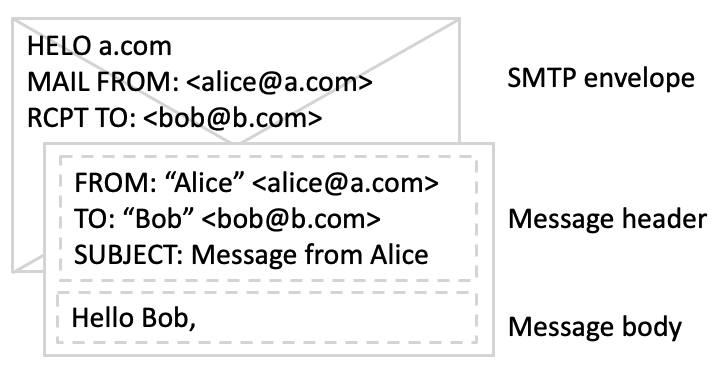
\includegraphics[width=\columnwidth]{fig/mech_smtp_headers.pdf}}
    \centering
    \caption{Example SMTP headers in a transmission (inspired by Figure 3 in Chen et al.~\cite{chen2020composition}).}
    \label{fig:mech_smtp_headers}
\end{figure}

\subsection{Email Spoofing Protections}
The original SMTP design lacks authentication, which
has made email spoofing attacks both possible and common. To mitigate these attacks, the community has proposed multiple mechanisms that focus on authenticating the \emph{domain name} used by the
purported sender.\footnote{True per-sender authentication has long floundered
  due to the lack of effective mechanisms for binding user identities
  with cryptographic credentials at scale.  The best known protocol in
  this space, PGP, has been riddled with security and usability issues
  and remains, at best, a niche protocol.  In this paper, we focus
  exclusively on domain-level sender authentication.} Of these
mechanisms, we focus on SPF~\cite{rfc7208}, DKIM~\cite{rfc6376}, and DMARC~\cite{rfc7489} given their wide adoption.

%\subsubsection{SPF}
\medskip
\noindent\textbf{Sender Policy Framework (SPF)} defines a list of IP addresses permitted to send email on behalf of a domain and a set of actions the recipient should take if they receive an email from an unauthorized IP address.\footnote{In addition to lists of raw IP addresses, SPF
records can also ``include'' other SPF records by reference.}
Domain owners specify this policy by publishing it in a DNS TXT record.
Upon receiving an email message, the receiver fetches the list of authorized sender IP addresses by querying the domain in the email's \textsc{MAIL FROM} header.
The recipient then verifies if the IP address of the sending server is included that list.
If the verification fails, the receiver enforces the action (e.g., marking the email as spam) specified by the \textsc{MAIL FROM} domain in their SPF policy.


% When receiving email from a given IP address, a mail server queries the
% domain present in the \textsc{MAIL FROM} header to obtain its SPF
% policy (encoded in DNS TXT records) and checks whether the policy's list of allowed IP addresses includes the sending server's IP address.
% If the check fails, the mail server then enforces the filtering policy
% specified by the domain owner's SPF policy (\eg, hard fail, soft fail).
% \footnote{Note, it is recommended but not required to also
  % check against the domain identified in SMTP's HELO handshake.}
%
% One major problem with SPF is that it is not compatible with simple
% forwarding. When an email is forwarded, SPF checks can fail because a
% mail server will authenticate the forwarding server, rather than the
% original sending server.

%\subsubsection{DKIM}
\medskip
\noindent\textbf{DomainKeys Identified Mail (DKIM)} cryptographically
binds an email message with its sending email domain.  With DKIM, the
sender signs an email (or certain elements of an email) and attaches a digital signature via a
\textsc{DKIM-Signature} message header for future verification.
Receivers later retrieve the signer's public key (in the form of a DNS TXT record) from the domain specified in the \textsc{DKIM-Signature} header and authenticate an email's signature using that key.

Sadly, neither SPF nor DKIM verify that an email's purported sender (\ie, the \textsc{FROM} header) truly wrote and sent it~\cite{chen2020composition}.
For example, an attacker could bypass DKIM by spoofing an email's \textsc{FROM} header, but then sign and attach a DKIM signature that uses key pairs linked to their own domain (since DKIM does not compare the signature's domain against the \textsc{FROM} domain).
Attacks that exploit
this lack of \textsc{FROM} header authentication motivated the creation of DMARC.
% the \textsc{FROM} header
% displayed to the users, and passing SPF and/or DKIM validation does
% not guarantee the authenticity of the \textsc{FROM} header.  This
% lack, among other reasons, led to the creation of DMARC.

%\subsubsection{DMARC}
\medskip
\noindent\textbf{Domain Message Authentication, Reporting, and
Conformance (DMARC)} combines and extends SPF and DKIM to mitigate these security issues.
% authenticate the domain specified in the \textsc{FROM} header. 
Under DMARC, an email's receiver performs an ``alignment test'': checking if the
domain in the \textsc{FROM} header matches the domain name verified by
either SPF (the domain in the \textsc{MAIL FROM} header) or DKIM (the
domain in the \textsc{DKIM-Signature} header).
By default (``relaxed mode''), the alignment test only requires that the registered domains in the headers match (\ie, not the fully qualified domain name (FQDN)). However, domain owners can specify that recipients should follow the strict mode of the alignment test, which requires the \textsc{FROM} header's FQDN to exactly match the domain authenticated by SPF or DKIM.\footnote{%As with SPF, 
DMARC policy records are also stored as DNS TXT records.} 

If the email passes either SPF or DKIM authentication, and the alignment test also passes, then DMARC considers the email authenticated.
% The alignment test, and overall DMARC authentication for an email, succeeds if 
% The alignment test succeeds if the email passes under either the SPF or DKIM comparison
% When either SPF or DKIM are successful and the alignment test is also successful, the email is considered passing DMARC authentication.
Otherwise, the receiver should implement the DMARC policy designated by the domain in the \textsc{FROM} header, selected from one of three options: \textsc{None},
\textsc{Quarantine}, or \textsc{Reject}.  A policy of \textsc{None}
specifies that an email should be delivered as normal (and thus is often used for monitoring purposes~\cite{DMARCMonitoring1,DMARCMonitoring2}), and \textsc{Reject}
specifies that the recipient mail server should drop the email without
delivering it to the user.  The \textsc{Quarantine} policy is not strictly
defined (indicating only that the message should be treated ``as
suspicious'') and allows each email provider considerable latitude in
their implementation (\eg, setting a UI indicator or placing the email
in a designated spam folder)~\cite{rfc7489}.

%\subsubsection{UI-level Protection}
%% \paragraph{UI Indicators}
%% The combination of these various measures does
%% not always produce a clear binary signal.
%% Thus, email services frequently combine filtering rules with application-layer user interface (UI) indicators to help alert users when the authenticity of an email is suspect.
%% However, currently there is no standard for how and when such
%% UI indicators should be implemented, and different providers favor
%% different approaches.
%% \grant{I think we can completely cut this paragraph if we need space (IV.D.2 gives enough context about UI defenses without this.)}
%% \geoff{looking at IV.D.2, agreed}
% \grant{This part is a little thin, and might be worth folding into the
% vulnerability/attack section where relevant.}\amirian{agreed; it seems out of
% place here. unless this specifically comes into play in the attack section I
% would consider removing it}

% So, in addition to mandatory
% filtering rules, application-layer user interface (UI) indicators are also
% commonly used to help alert users when the authenticity of an email is
% suspect. However, currently there is no standard on how and when such
% UI indicators should be implemented, and different providers favor
% different approaches.

% (1) {\bf
% p=reject} the mail server rejects the email (2) {\bf p=quarantine} the mail
% server accepts the email but marks it as suspicious\gakiwate{Put it in Trash?}
% (3) {\bf p=none} the mail server accepts the email
% nevertheless.\gakiwate{@@Alex: spell out the DMARC policies and expected behavior}

% The DMARC policy None is the weakest and allows for spoofing since an email
% maybe accepted regardless of whether it passes SPF or DKIM. That said, most
% email providers will label such emails as suspicious and display warnings.
% Thus, even though a domain may have DMARC policy None an attacker still may
% have to defeat email providers' protections to deliver an email to the users
% inbox.

% \gakiwate{@@Alex: Make consistent with dmarc policy usage elsewhere.}

% Together these mechanisms can help authenticate emails and thus prevent the
% email spoofing.
%Next, we consider email forwarding and how it complicates these
%email authentication mechanisms.

\begin{figure}[t]
%  \vspace*{-0.2in}
\centerline{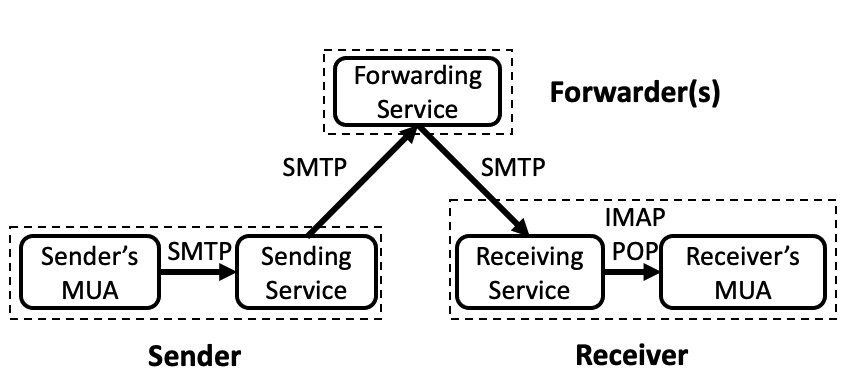
\includegraphics[width=\columnwidth]{fig/mech_email_forwarding_flow.pdf}}
\caption{Email flow involving forwarding.}
\label{fig:email_forwarding_flow}
  \vspace*{-0.1in}
\end{figure}


\subsection{Email Forwarding}
\label{sec:background:fwd:overview}
% \amirian{can you give a one sentence example of a e.g. of a forwarder? someone
% who isnt familiar with forwarders might not understand who can run them and it
% would help to cement the understanding here}
Forwarding is ubiquitous in the email ecosystem and is necessitated by
the wide use of mailing lists~\cite{Electron8:online}, email filtering
services such as ProofPoint~\cite{SecureEm78:online}, and
auto-forwarding employed by individual users for account
aggregation~\cite{TheBestW9:online}, among others.  As shown in
Figure~\ref{fig:email_forwarding_flow}, forwarding alters the standard
transmission flow of an email message.  Instead of a direct
transmission from the sender to the recipient, forwarding relays an
email from the sender to an intermediate server and/or account, which
then transmits a copy of the email to the final recipient.
% (e.g., when a student configures her university email account to forward all messages to a pre-existing personal email address).
For simplicity we show a single forwarder in our example, but email can pass through multiple forwarders in common use cases. % (note, while the figure shows a single forwarder, it is possible to have multiple such forwarders in series).
%While Figure~\ref{fig:email_forwarding_flow}
%shows a single forwarder it is possible to have multiple forwarders.
%Additionally, a forwarder may not always have a domain name associated with it.
%\gakiwate{@@Alex: ProofPoint does not have a domain name no? Check.}

% Forwarders play the same role as receivers but also seek to
% retransmit the original message to a new destination.
Like normal receivers in direct mail transfer,
forwarders are responsible for performing standard authentication checks on each email they receive. % as normally done by a receiver.
However, after authenticating a message,
a forwarder often makes \emph{changes} to the email headers and/or the
email body based on the service it provides.
%(\S~\ref{sec:measure_forwarding_mechs_and_arc}).
The forwarder then sends the modified message to the final receiver (or next forwarder), which also performs authentication checks upon receiving the email.
Finally, when a recipient receives and opens an email, the receiver's user agent (MUA) parses and displays the message to the user.
%If such an email fails DMARC authentication checks at the receiver, the receiver should follow the DMARC policy specified in the email's \texttt{FROM} header.
% Finally, an email is parsed and displayed at the recipient's mail user
% agent.

%. Additionally, most email providers add their own
%warnings if needed based on the email. While an email contains
%multiple headers that represent different sender identities, the MUA
%generally only displays the FROM header and optionally displays other
%headers~\cite{chen2020composition}.
%
% However, the need to accommodate email forwarding while reliably
% authenticating emails introduces challenges. For example, SPF
% validation frequently fails because the receiver will attempt to
% authenticate the forwarding service (which frequently does not have
% the same domain as the \textsc{MAIL FROM} header) rather than the
% original sending server.  Moreover, DKIM checks may fail if a
% forwarder modifies the email body (\eg, many mail filtering services
% rewrite URLs in the email body to offer post-delivery protection). The
% resulting DMARC failures may thus prevent forwarded mail from being
% delivered (\ie, if the \textsc{FROM} domain DMARC policy is quarantine or
% reject).  To prevent this outcome, and preserve the utility of
% forwarders, forwarding services modify email headers to try to ensure
% email delivery. Unfortunately, there is no accepted standard for these
% modifications and different providers use different strategies ---
% \emph{forwarding mechanisms} --- to forward email.  We describe four
% such forwarding mechanisms
% (Figure~\ref{fig:forwarding_mechs_combined}) that are relevant to this
% paper. While some mechanisms are well-documented (\eg, remailing),
% others are ad-hoc and not as well-documented.

%while others are custom and less well-documented \alex{e.g. MAIL FROM equals
%FROM, which is used by outlook}.

% %\subsubsection{Email Forwarding Mechanisms}
% \begin{figure}[t]
%     \centering
%     \includegraphics[width=\columnwidth]{graphs/table_forwarding_mechanisms_combined.png}
%     \caption{Four Types of Forwarding Mechanisms}
%     \label{fig:forwarding_mechs_combined}
% \end{figure}
%
% \noindent{\bf Plain Message-Forwarding (PMF)}. Initially designed for
% the purpose of ``source-routing''~\cite{Emailfor45:online}, PMF was
% one of the first forwarding mechanisms in wide use.  PMF only changes
% the \textsc{RCPT TO} header and leaves other fields
% untouched~\cite{Emailfor45:online} when forwarding.
% Figure~\ref{fig:forwarding_mechs_combined}a depicts the actions of
% such a forwarder which changes the \textsc{RCPT TO} header to the
% address of the receiver (\dns{c@c.com}) and leaves all other fields
% intact.
%
% In general, SPF disallows PMF, since this style of forwarding often
% causes SPF checks to fail at the final receiver.  Nevertheless, as we
% detail later, many email providers, like Yahoo and Fastmail, still use
% PMF in practice, which can result in security issues.
%
% {\bf Remailing (REM)}. Compared to PMF, remailing (aka redistribution),
% works well with SPF. It refers to re-sending a message and also
% rewriting the \textsc{MAIL FROM} field. It is commonly named remailing
% because the process resembles the action of a Mail User Agent
% submitting a new
% message\cite{SenderRe69:online}. Figure~\ref{fig:forwarding_mechs_combined}b
% depicts an example of how headers are modified in remailing. The
% forwarder (\dns{b.com}) first changes the \textsc{RCPT TO} header
% to reflect the destination email address (\dns{c@c.com}). It also
% rewrites the \textsc{MAIL FROM} header to reflect an address in its
% own domain (e.g., \dns{xyz@b.com}).\footnote{The exact username (the
%   ``xyz'' part) in the \textsc{MAIL FROM} address after rewriting
%   depends on the specific implementation.}  The Sender Rewriting
% Scheme, defined in RFC 5231~\cite{rfc5231}, provides a generic
% framework for rewriting email addresses in the \textsc{MAIL FROM}
% header. However, in reality, providers do not strictly follow this
% scheme.
%
% While REM works for well for SPF, it is not very compatible with
% DMARC. Without a valid DKIM header, which can happen sometimes (\eg,
% mailing lists alter a user's post signed by DKIM~\cite{rfc6783}), email
% messages forwarded via REM would fail DMARC's alignment test, and thus
% DMARC authentication. This creates a problem if the \textsc{FROM}
% domain has strict DMARC policies like quarantine or reject.
%
% \noindent{\bf Remailing with Modification (REM + MOD)}. Email
% forwarded by mailing lists that exercise REM and also alter message
% content can also sometimes fail DMARC. Remailing with Modification (REM +
% MOD) was introduced to address this issue and ensures forwarded email
% messages will pass SPF and DMARC. Besides modifying the headers
% mentioned in REM, REM + MOD also rewrites the \textsc{FROM}
% header~\cite{rfc6783}.  Figure~\ref{fig:forwarding_mechs_combined}c
% shows an example of such a modification.  Here, a forwarder
% (\dns{b@b.com}) modifies \textsc{MAIL FROM} and \textsc{RCPT TO}
% headers like REM.  Additionally, it changes the \textsc{FROM} header
% to an email address in its own domain (\dns{b@b.com}).
%
% While fully compatible with DMARC, for the same reason REM + MOD also
% introduces new security concerns. A spoofed email forwarded via REM +
% MOD is ``laundered'' with a new set of headers that will always pass
% SPF and DMARC checks, making it no different than other legitimate
% email messages.
%
%
% \noindent{\bf MAIL FROM Equals From (MFEF)}. Unlike the three
% forwarding mechanisms described above, for which we can find some
% public documentation, MAIL FROM Equals From is a custom forwarding
% mechanism that appears to only be used by Outlook.\footnote{We are not
%   entirely clear what function MFEF serves but we hope, as part of our
%   disclosure interactions with Microsoft, to gain a better
%   understanding of this design's motivation for a future version of
%   this paper.}  An example of MFEF is shown in
% Figure~\ref{fig:forwarding_mechs_combined}d.  In addition to rewriting
% the \textsc{RCPT TO} header to reflect the final receiver
% (\dns{c@c.com}), the forwarder also sets the \textsc{MAIL FROM}
% header to be the same as the \textsc{FROM} header (\dns{a@a.com}),
% regardless of the original \textsc{MAIL FROM} header
% (\dns{z@a.com}). In many scenarios, like PMF, MFEF also will break
% SPF.
%
% %\subsection{Authenticating Email Forwarding}
% %\gakiwate{Can this be confused with simple email forwarding. fwd:
% %  kind?}  As we previously discussed, email authentication using SPF,
% %DKIM and DMARC may lead to email deliverability issues. Thus,
% %forwarders may modify email headers before forwarding to ensure the
% %authentication checks still work.  As such, the receiver implicitly
% %relies on the intermediate forwarders to authenticate the email before
% %modifying it and sending it along.  However, as we demonstrate
% %(Section~\ref{sec:vulnerabilities_in_the_wild}) these assumptions may
% %not always
%
% %For example, an adversary could coax a
% %legitimate forwarder to forward a spoofed email by manually whitelisting domains
% %(Section~\ref{subsec:attack_open_forwarding}). Perhaps more egregiously, some
% %forwarders do not enforce DMARC and forward every email they receive
% %(Section~\ref{subsec:vul:no_dmarc}). Moreover, even the receiver could
% %incorrectly handle the authentication of forwarded emails
%
% \subsection{Authenticated Received Chain}
% \label{sec:arc}
%
% Given the limitations of SPF, DKIM, and DMARC in the presence of
% forwarding, a new mechanism called Authenticated Received Chain
% (ARC)~\cite{rfc8617} was recently introduced to preserve email
% authentication results across multiple forwarders.  ARC chains enable
% a receiver, who might otherwise discard a message, to evaluate the
% full set of intermediary forwarders involved in transmitting the email
% in order to make appropriate exceptions and allow legitimately
% forwarded messages to be delivered~\cite{ARCSpeci1:online}.
%
% %ARC was proposed to solve the deliverability issue introduced by forwarding.
% Intermediary hops implementing ARC sign their authentication results
% (using ARC specific headers) so that these results are accessible by the
% receiver. The expectation is that, in the case where DMARC authentication fails,
% if an ARC chain is present
% %and validated,
% a receiver might choose to
% evaluate the ARC results and allow legitimate emails to be delivered.
%
% However, ARC is currently an experimental standard and only
% implemented by a few providers~\cite{rfc8617, ARCSpeci1:online}. Among
% these, many providers maintain a list of trusted forwarders that
% implement ARC~\cite{Senderau57:online} instead of trusting all
% ARC forwarders. However, any such trust implicitly
% assumes that those trusted forwarders have good security practices.
% Unfortunately, as we detail later, this is not always the case, which
% creates additional opportunities for adversaries
% (Section~\ref{subsec:attack_zoho_arc}).

\subsection{Related Work}

Email security has been a long-standing problem and a variety of prior research efforts have examined different aspects of it. One line of work focuses on understanding and defending against phishing attacks. This includes papers that design new tools for detecting both traditional phishing and sophisticated spearphishing attacks~\cite{abu2007comparison,bergholz2008improved, fette2007learning, garera2007framework, whittaker2010large, duman2016emailprofiler, khonji2011mitigation, zhao2016optimizing, stringhini2015ain, ho19, ho17, cidon19},
study the characteristics of real-world phishing attacks~\cite{han2016phisheye,onaolapo2016happens,thomas2014consequences,bursztein2014handcrafted}, and examine the human aspect of such attacks~\cite{lastdrager2017effective, reinheimer2020investigation,abu2007comparison,
mayer2022don,caputo2013going,
Spero20, Sheng10, Kumaraguru10}.

Another body of work investigates the security and deployment of email encryption mechanisms, such as PGP~\cite{muller2019johnny, poddebniak2018efail, schwenk2020mitigation, muller2020mailto,stransky202227}, DANE~\cite{lee2022under,lee2020longitudinal}, and STARTTLS~\cite{zakir15,Foster15,poddebniak2021tls,holz2015tls,mayer2016no}.

A third research direction analyzes the security and deployment of anti-spoofing protocols such as SPF, DKIM and DMARC, with efforts from both industry and academia. The blogposts by Ullrich~\cite{Breaking12:online} and Haddouche~\cite{Mailsplo10:online} investigated approaches for bypassing DKIM and DMARC using malformed email messages.
Other work has empirically measured the efficacy and deployment status of SPF, DKIM, and DMARC~\cite{hu_end--end_nodate, zakir15, Foster15, tatang2021evolution, deccio21, wang2022large, bennett2022spfail}, as well as qualitatively characterized the factors that drive DMARC policy decisions~\cite{hutowardsunderstanding}.
% systematically researched the deployment of SPF, DKIM and DMARC, including
% the empirical study by Hu \etal\ of anti-spoofing efficacy among
% providers, a subsequent qualitative study
% to investigate the
% factors that
% drive DMARC policy decisions~\cite{hutowardsunderstanding}, and empirical measurement studies of the deployment of SPF, DKIM and DMARC by Durumeric et al.~\cite{zakir15}, Foster et al.~\cite{Foster15}, Tatang et al.~\cite{tatang2021evolution}, Deccio et al.~\cite{deccio21} and Wang et al.~\cite{wang2022large}.

The work most related to our own includes Chen et al.'s analysis of
the security vulnerabilities introduced by protocol composition in
modern email delivery~\cite{chen2020composition}, Shen et al.'s
analysis~\cite{shen2020weak} of modern sender spoofing attacks, and Wang et al.'s~\cite{wang2022revisiting} analysis of email security under the experimental Authenticated Received Chain (ARC) protocol~\cite{rfc8617}.
Of these, Chen et al.~\cite{chen2020composition} do not consider forwarding at all and Wang et al.~\cite{wang2022revisiting} focus on ARC and only consider one specific forwarding implementation as well (REM+MOD in Section~\ref{sec:measure_forwarding_mechs_and_arc}), leaving many other vulnerable forwarding mechanisms and features unexplored.

Shen et al.'s work~\cite{shen2020weak} is the closest in that it also
examines open forwarding, but because they only consider one
forwarding mechanism (what we label as REM in
Section~\ref{sec:measure_forwarding_mechs_and_arc}), they do not
identify the significant scope of this issue.  We build on and
generalize this work to show, among other attacks, that attackers are
able to practically abuse open forwarding to spoof \emph{any} domain
that includes the forwarding domain's SPF record in their own SPF record (a
common practice when hosting email via Microsoft's Outlook service for example).

% and does not illuminate many of the attacks described in our work.
% in Section~\ref{subsec:attack_open_forwarding}

%Additionally, we show how a bug they disclosed in Zoho's ARC implementation, they did not demonstrate how to use this vulnerability in practical attacks.
% due to their limited scope
%In contrast, we present a viable attack that allows an adversary to deliver spoofed email messages addressed from arbitrary domains to arbitrary Zoho users (Section~\ref{subsec:attack_zoho_arc}).
% Similarly, while they were the first to disclose Zoho's buggy ARC implementation, they missed the attack we describe in Section~\ref{subsec:attack_zoho_arc} due to limited scope --- that they only examined ARC in the context of Gmail and Zoho and did not consider forwarding configurations, which are critical components that enable the attack.

In summary, our work builds on the insights of prior efforts, but focuses exclusively and deeply on the particular security challenges introduced by the design and features of common forwarding mechanisms, and their complex interactions with existing email protocols. Through systematic measurements and analysis, we not only show that prior work largely underestimates the risks of open forwarding,
% (Section~\ref{subsec:attack_open_forwarding}),
but also reveal new attacks not discovered in prior work.
%(Section~\ref{sec:attacks}).



%Since
%forwarding is not the main focus of Shen et al.~\cite{shen2020weak},
%they only present a limited set of results: (1) their forwarding
%mechanism is limited to REM, understating many of the potential
%security issues (2) They examine open forwarding in the context of
%REM, (3) they do not elaborate on capacity of attacks introduced by
%certain vulnerabilities (\eg, the Zoho bug). (4) their work is limited
%to mail providers. In comparison, our work: (1) performs a systematic
%and empirical analysis of forwarding mechanisms used in wild,
%discovering three other broad types of forwarding mechanisms (2)
%Comprehensively measures vulnerabilities exist at all parties involved
%in the email forwarding flow \alex{we omit vulnerabilities they
%  discovered but not used in our attacks} (3) Uncovers security issues
%associated with certain vulnerabilities that are understated (\eg,
%open forwarding and Zoho's ARC bug). Our work also leads to a patch of
%the ARC bug by Zoho (\S~\ref{sec:disclosure}). (4) We also consider
%security issues centered around another common use case of forwarding
%--- mailing lists.

%Besides~\cite{shen2020weak}, other work has talked about different
%ways of bypassing email security protocols. For example,

%\alex{Phishing citations cam be added later}


\section{Email Forwarding in Practice}
% \section{The Challenges with Email Forwarding}
\label{sec:measure_forwarding_mechs_and_arc}

Despite the ubiquity of email forwarding, there is no single and
universally agreed-upon method for how email services should implement
forwarding, resulting in several different approaches~\cite{Emailfor34:online}.  This
heterogeneity stems in part from the difficulty of balancing
compatibility with anti-spoofing protocols and the functional goals of
many forwarding use cases: to transparently hide the intermediate
forwarder and present the illusion that the recipient receives the
email directly from its original sender.

Absent a clear standard to depend on, we have used empirical
measurements to \emph{infer} the forwarding behavior deployed by
prominent email providers and mailing list services.  For each
service, we created multiple test accounts, used them to forward email
to recipient accounts we controlled, and then analyzed the resulting
email headers to identify the forwarding mechanism employed.
(Section~\ref{sec:methodology} has a more detailed description of our
methodology.)

We constructed a comprehensive and representative set of forwarding services by building on top of prior literature.
In total, we studied 20 distinct, leading email forwarding services.
We started by collecting all email providers studied in prior literature~\cite{chen2020composition,shen2020weak,hu_end--end_nodate,wang2022revisiting}.
We considered an email provider \emph{out of scope} if it meets any of these four criteria: (a) it is no longer active (e.g., excite.com); (b) it does not accept US customers (e.g., all Chinese providers studied in prior work);  (c) it is not open to public registration (e.g., cock.li); or (d) it does not support forwarding (e.g., Protonmail).
Using these criteria, we identified 23 email providers.
Next, we excluded five email providers that prohibited bulk registration (which prevents us from running large-scale measurements), leaving us with 18 email providers.
We then identified and removed duplicate providers that are operated by the same vendor under different names, leading to a total of 14 distinct email providers.
Finally, we augmented this set of forwarding services by searching for popular email providers that supported forwarding and widely-used mailing list services (a common use case overlooked in prior literature), adding two additional email providers (Mail2World and GoDaddy) and four mailing lists.

Our selection of email forwarding services covers a diverse set of countries and real-world use cases (personal and business email), and represents services used by the general public (used by over 46\% of popular Alexa domains and government domains according to Liu et al.~\cite{liu2021s} ignoring email filtering services).
%\alex{42.7\% considering email filtering}. 
We list all email providers and mailing lists in Table~\ref{tab:forwarding_mechs_in_the_wild}.


Through our measurements, we confirmed the use of three common
approaches that are generally known through public documentation, and
identified a fourth uncommon implementation used by
Microsoft Outlook (hence referred to as Outlook) and Freemail.hu (hence referred to as Freemail).
As summarized in
Figure~\ref{fig:forwarding_mechs_combined}, in each approach the
forwarder modifies the sender and recipient fields in the SMTP
Envelope and Message headers before relaying the email to its
recipient.



% By analyzing public documentation and empirically testing popular email services (\S~\ref{sec:fwd_adoption_measurement}), we identified four major approaches to implementing email forwarding.
% \geoff{is this a ``result'' because Microsoft's implementation has to be experimentally discovered?}\alex{it is technically discovered through experiments}

We now describe each of these approaches in detail using two running
examples of common email forwarding use cases.  In the first case,
Alice has configured her university account (\dns{alice@univ.edu}) to
forward to her primary personal account (\dns{alice@gmail.com}).  When
her university account receives email (\eg, from
\dns{sp@hotcrp.com}), forwarding retransmits it to
\dns{alice@gmail.com} in a way that makes it seem like the email comes
directly from the sender (\dns{sp@hotcrp.com}), rather than from her
university account.  In the second case, Bob sends an email to a
mailing list (\dns{list@univ.edu}), which redistributes (forwards) the
email to the list's members (\eg, \dns{user@univ.edu}).


\begin{figure}[t]
  \centering
%  \vspace*{-0.1in}
    \includegraphics[width=0.7\columnwidth]{fig/table_forwarding_mechanisms_combined.pdf}
    \caption[Four Prevalent Approaches to Email Forwarding]{Four prevalent approaches to email forwarding.  Addresses
      in blue correspond to header values rewritten during the
      forwarding process.
      }
    \label{fig:forwarding_mechs_combined}
\end{figure}


% \grant{In MFEF, is there a reason why the MAILFROM is acm instead of hotcrp? If it's to illustrate a change, I suggest we use noreply@hotcrp.com for the sender MAIL FROM addresses.}\alex{fixed}

% \noindent{\bf Plain Message-Forwarding (PMF)}.
\textbf{Plain Message-Forwarding (PMF)}. Initially designed for
the purpose of ``source-routing''~\cite{Emailfor45:online}, PMF was
one of the first forwarding mechanisms in wide use.
Forwarders that use PMF only change
the \textsc{RCPT TO} header from the forwarder's email account (\dns{alice@univ.edu}) to the final recipient's address (\dns{alice@gmail.com}), and leave all other fields
untouched,
%~\cite{Emailfor45:online},
as illustrated in Figure~\ref{fig:forwarding_mechs_combined}a.
This approach achieves the goal of transparent forwarding.
Changing the \textsc{RCPT TO} header will tell mail servers to send the email to the new address's account, and leaving the \textsc{FROM} header intact will
cause the recipient's email client to display the initial sender (\dns{sp@hotcrp.com}),
rather than presenting \dns{alice@univ.edu} as the sender.
% This approach achieves the goal of transparent forwarding, since the email will appear to come from its initial sender (the \textsc{FROM} header displays the original sender).
% However, it will cause SPF validation to fail in many cases, since the \textsc{MAIL FROM} domain may not list the forwarding server's IP address in its SPF allowlist.


% \noindent{\bf MAIL FROM Equals From (MFEF)}.
\textbf{MAIL FROM Equals FROM (MFEF)}.
Similar to PMF, MFEF (Figure~\ref{fig:forwarding_mechs_combined}b) aims to achieve transparent forwarding by preserving the original sender's identity in the \textsc{FROM} header.
Unlike the other forwarding approaches described in this section, MFEF is a custom forwarding implementation that appears to be used only by Outlook and Freemail.
% \footnote{We are not
%   entirely clear what function MFEF serves but we hope, as part of our
%   disclosure interactions with Microsoft, to gain a better
%   understanding of this design's motivation for a future version of
%   this paper.}
A MFEF forwarder not only rewrites the \textsc{RCPT TO} header to the final recipient (\dns{alice@gmail.com}), but it \emph{also} sets the \textsc{MAIL FROM}
header to be the same as the \textsc{FROM} header (from \dns{noreply@hotcrp.com} to \dns{sp@hotcrp.com}).

Email forwarded using PMF and MFEF often break SPF validation because the \textsc{MAIL FROM} domain typically does not list the forwarding server's IP address in its SPF allowlist;
in our example, \dns{hotcrp.com} does not list the email servers for \dns{univ.edu} in its SPF allowlist.
This incompatibility has hindered the adoption of SPF and DMARC~\cite{hutowardsunderstanding},
leading to provider-specific defenses and new anti-spoofing protocols that we describe in Section~\ref{sec:assumptions}.

%Despite these defenses, we show how attackers can abuse forwarding to nonetheless successfully spoof email from hundreds of thousands of popular domains in
%Section~\ref{sec:attacks}.

% Figure~\ref{fig:forwarding_mechs_combined}a depicts the actions of
% such a forwarder which changes the \textsc{RCPT TO} header to the
% address of the receiver (\dns{c@c.com}) and leaves all other fields
% intact.

% In general, SPF disallows PMF, since this style of forwarding often
% causes SPF checks to fail at the final receiver.  Nevertheless, as we
% detail later, many email providers, like Yahoo and Fastmail, still use
% PMF in practice, which can result in security issues.

% {\bf Remailing (REM)}.
\textbf{Remailing (REM)}. Unlike PMF and MFEF, remailing (aka redistribution)
works well with SPF because this approach alters the headers in a way that resembles the action of the forwarder submitting a new message~\cite{SenderRe69:online}.
% It refers to re-sending a message and also
% rewriting the \textsc{MAIL FROM} field. It is commonly named remailing
% because the process resembles the action of a Mail User Agent
% submitting a new
% message\cite{SenderRe69:online}.
As shown in Figure~\ref{fig:forwarding_mechs_combined}c, the REM
forwarder (\dns{univ.edu}'s mail server) first changes the
\textsc{RCPT TO} header to specify the final recipient (\dns{alice@gmail.com}).
Additionally, the forwarder rewrites the \textsc{MAIL FROM} header so that it
corresponds to an address in the forwarder's own domain (\eg,
\dns{alice-xyz@univ.edu}).\footnote{The Sender Rewriting Scheme
(RFC~5231~\cite{rfc5231})provides a generic framework for how forwarders should
rewrite the \textsc{MAIL FROM} header.  However, email providers do not
strictly follow this scheme and the exact email address after rewriting varies
by implementation.}
% \footnote{The exact username of the \textsc{MAIL FROM} address after
% rewriting varies by the specific implementation.}  The Sender Rewriting
% Scheme, defined in RFC 5231~\cite{rfc5231}, provides a generic
% framework for rewriting email addresses in the \textsc{MAIL FROM}
% header. However, in reality, providers do not strictly follow this
% scheme.

However, even though REM interoperates with SPF, it can still fail DMARC
authentication.  Absent a valid DKIM header, email messages forwarded
via REM will fail DMARC's alignment test because the \textsc{FROM}
domain will not match the SPF-verified \textsc{MAIL FROM}
domain.\footnote{Many domains still do not implement DKIM for outbound email, and even
  those that do can have their user's DKIM signatures invalidated by mailing
  list software that adds content to a user's post~\cite{rfc6783}.}
This incompatibility has led to the common adoption of weaker DMARC policies,
such as \textsc{None} and \textsc{Quarantine} instead of
\textsc{Reject}~\cite{hutowardsunderstanding}.

% This creates a problem if the \textsc{FROM}
% domain has strict DMARC policies like quarantine or reject.

% \noindent{\bf Remailing with Modification (REM + MOD)}.
\textbf{Remailing with Modification (REM + MOD)}.
The final forwarding approach, Remailing with Modification (REM + MOD)~\cite{rfc6783},
resolves these compatibility issues by sacrificing the goal of transparent forwarding.
Email forwarded using REM + MOD will pass both SPF and DMARC.
However, email forwarded with this approach will display the \textit{forwarder} as the email's sender to the final recipient (hiding the identity of the original sender).
Because of this functional change, most major email platforms do not adopt this approach, and it is used primarily by mailing list services such as Gaggle.

As shown in Figure~\ref{fig:forwarding_mechs_combined}d, with REM + MOD the forwarder modifies the headers just like it would during REM forwarding: changing the \textsc{RCPT TO} header to the final recipient (\dns{user@univ.edu}) and the \textsc{MAIL FROM} header to an address in the forwarder's domain.
Additionally, the forwarder rewrites the \textsc{FROM} header to match its account or an email address within its domain (e.g., \dns{list@univ.edu}).

Although this forwarding approach produces email messages compatible with DMARC,
we found that it also introduces a new set of security concerns and spoofing attacks (\S~\ref{subsec:attack_none_mailing_list}).
At a high-level, because REM + MOD rewrites a forwarded email's headers to always pass SPF and DMARC checks, it enables an attacker to launder a spoofed email through a vulnerable forwarder such that it appears like a legitimate email message to the recipient.

% To resolve these compatibility issues with security protocols,
% one forwarding approach, Remailing with Modification (REM + MOD), choses to sacrifice the goal of transparent forwarding to ensure that forwarded emails pass both SPF and DMARC.
%
% As seen in Figure~\ref{fig:forwarding_mechs_combined}c, during REM + MPD, the forwarder modifies the headers just like it would during REM forwarding: changing the recipi
%
% Remailing with Modification (REM + MOD) allows emails to pass both SPF and DMARC, however the emails forwarded under this approach will display the forwarder as the email's sender to the final recipient (hiding the identity of the original sender).
%
% Email forwarded by mailing lists that exercise REM and also alter message
% content can also sometimes fail DMARC. Remailing with Modification (REM +
% MOD) was introduced to address this issue and ensures forwarded email
% messages will pass SPF and DMARC. Besides modifying the headers
% mentioned in REM, REM + MOD also rewrites the \textsc{FROM}
% header~\cite{rfc6783}.
%
% Figure~\ref{fig:forwarding_mechs_combined}c
% shows an example of such a modification.  Here, a forwarder
% (\dns{b@b.com}) modifies \textsc{MAIL FROM} and \textsc{RCPT TO}
% headers like REM.  Additionally, it changes the \textsc{FROM} header
% to an email address in its own domain (\dns{b@b.com}).

% While fully compatible with DMARC, for the same reason REM + MOD also
% introduces new security concerns. A spoofed email forwarded via REM +
% MOD is ``laundered'' with a new set of headers that will always pass
% SPF and DMARC checks, making it no different than other legitimate
% email messages.

% \begin{table}[t]
% \centering
% \begin{tabular}{lll}
% \toprule
% \textbf{Provider} & \textbf{Fwd. Mechanism} & \textbf{ARC} \\
% \midrule
% Gmail         & REM                & \checkmark            \\
% Outlook       & MFEF               & \checkmark            \\
% Zoho      & REM                & \checkmark            \\
% Fastmail      & PMF                & \checkmark            \\
% Yahoo         & PMF                &             \\
% GMX           & REM                &             \\
% Mail.Ru           & PMF                &             \\
% Inbox.lv           & REM                &             \\
% Mail2World.com           & PMF                &             \\
% \midrule
% Google Groups & REM          & \checkmark            \\
% Gaggle  & REM + MOD          &             \\
% Listserv      & REM                &             \\
% Mailman       & REM                & \checkmark \\
% \bottomrule
% \end{tabular}
% \caption{Default forwarding mechanisms and ARC support of the providers and mailing list services we tested.
% \grant{Let's remove the ARC column?}\alex{ok}
%   \label{tab:forwarding_mechs_in_the_wild}}
% \end{table}


%% \begin{table}[t]
%%   \centering
%%   \begin{tabular}{ll}
%%   \toprule
%%   \textbf{Provider} & \textbf{Forwarding Approach}  \\
%%   \midrule
%%   Gmail         & REM                       \\
%%   Outlook       & MFEF                        \\
%%   Zoho      & REM                          \\
%%   Fastmail      & PMF                         \\
%%   Yahoo         & PMF    \\
%%   GMX           & REM    \\
%%   Mail.Ru           & PMF     \\
%%   Inbox.lv           & REM   \\
%%   Mail2World.com           & PMF    \\
%%   \midrule
%%   Google Groups & REM            \\
%%   Gaggle.email  & REM + MOD         \\
%%   Listserv      & REM        \\
%%   Mailman       & REM       \\
%%   \bottomrule
%%   \end{tabular}
%%   \caption{Default forwarding mechanisms and ARC support of the providers and mailing list services we tested.
%%     \grant{The other/alternate version looks great (and uses less room than this)!}
%%     \geoff{I'll experiment with alternate formats}
%%     \label{tab:forwarding_mechs_in_the_wild}}
%%   \end{table}

\begin{table}[t]
  \centering
  \begin{tabular}{ll|ll}
  \toprule
\multicolumn{2}{l}{\textbf{Email} \hfill \hspace*{0.22in}\textbf{Forwarding}} & \textbf{Mailing} & \textbf{Forwarding} \\
\multicolumn{2}{l}{\textbf{Provider} \hfill \hspace*{0.05in}\textbf{Mechanism}} & \textbf{List Service} & \textbf{Mechanism} \\
  \midrule
  Fastmail        & PMF  & Gaggle & REM+MOD \\
  Freemail.hu     & MFEF & Google Groups & REM\\
  GMX/Mail.com    & REM  & Mailman & REM  \\
  Gmail           & REM  & Listserv & REM \\
  GoDaddy         & REM  & & \\
  Hushmail        & PMF  & & \\
  iCloud          & PMF  & & \\
  Inbox.lv        & REM  & & \\
  Mail.ru         & PMF  & & \\
  Mail2World      & PMF  & & \\
  Onet.pl/Op.pl   & REM  & & \\
  Outlook/Hotmail/O365 & MFEF & & \\
  Pobox           & REM  & & \\
  Runbox          & PMF  & & \\
  Yahoo           & PMF  & & \\
  Zoho            & REM  & & \\
  \bottomrule
  \end{tabular}
  \caption[The Providers and Mailing List Services Tested]{The providers and mailing list services we tested and the forwarding mechanisms they use. For providers that are operated by the same vendor under different names (e.g., GMX and Mail.com), we merge them into one row. O365 stands for Office 365.
    \label{tab:forwarding_mechs_in_the_wild}}
  %\vspace*{-0.2in}
  \end{table}

%\subsection{Adoption of Forwarding Approaches}
%\label{sec:fwd_adoption_measurement}

% % We used controlled experiments to evaluate the forwarding behavior of
% % nine prominent email providers
% % and four popular mailing list services.
% We empirically assessed which forwarding strategy different prominent email providers and mailing list servers have adopted.
% %\footnote{
% Our goal was to cover as many providers as possible that are studied
% in prior
% work~\cite{chen2020composition,shen2020weak,hu_end--end_nodate}, while
% filtering out providers that do not support forwarding.  We also skipped
% providers for which we had trouble registering accounts due to
% specific registration requirements (\eg,
% all Chinese providers), for which we could not bypass bot detection
% (\eg, Yandex), and those that make bulk registration challenging (\eg,
% iCloud). Notably, we study Google and Microsoft, which are prominent
% among popular domains according to Liu \etal~\cite{liu2021s}.
% \geoff{the current description is subtractive; another approach
%   is to have it be additive (cover prominent according to Liu +
%   mailing lists), and then describe that there are others we tried
%   for additional coverage but had the issues listed}\alex{I kinda like the additive one. See below}

% \alex{Additive version}

Table~\ref{tab:forwarding_mechs_in_the_wild} summarizes the default forwarding approach used by each of the email providers and mailing lists in our study.\footnote{A provider might forward differently when forwarding between internal accounts, and a mailing list might switch to a different forwarding mechanism to avoid issues caused by forwarding email messages from domains with stricter DMARC policies~\cite{spamreso59:online}. We do not consider these two cases.}
%
% \subsection{Default Forwarding Mechanisms}
% \label{subsubsec:measure_fwding_mech}
%
The most common forwarding approach is remailing forwarding (REM),
used by seven email providers (GMX, Gmail, GoDaddy, Inbox, Onet, Pobox, and Zoho) and
three mailing lists (Google Groups, Listserv, and Mailman). Seven email providers, Fastmail, Hushmail, iCloud, Mail.ru, Mail2World, Runbox, and Yahoo, use
plain-message forwarding (PMF).
% while
Outlook and Freemail use their own custom
forwarding mechanism (MFEF) and, as described, Gaggle uses remailing with modification (REM+MOD)
forwarding.
% \geoff{would ``Gaggle Mail'' be more consistent with how we name providers?}
% described in Section~\ref{sec:background:fwdingmechanisms}.

%% \begin{table*}[t]
%%     \centering
%%     \begin{tabular}{p{17em}p{14em}p{14em}}
%%         \toprule
%%     \textbf{Assumption or Feature}                          & \textbf{Associated Implementation}  & \textbf{Prevalence}    \\
%%     \midrule
%%     Domain will use actionable DMARC policies   & DMARC none & Two thirdsSecurity of popular Alexa domains that have DMARC \\
%%     %\hline
%%     Each domain uses its own infrastructure  & Shared SPF record    & All providers \alex{Fastmail? Forwarding infra?}  \\
%%     Quarantining an email neutralizes its threat    & Quarantine instead of reject    & Outlook, Fastmail, GMX and Inbox.lv \\
%%     Allowing users to override DMARC decisions    & Domain whitelisting    & All providers  \\
%%     %\hline

%%     Users only forward to accounts they control   & Open forwarding    & Outlook, Fastmail and Mail2world.com \\
%%     Forwarded email from large providers are likely benign  & Relaxed validation & Gmail, Outlook and Mail.ru   \\
%%     %    & Overtrust other providers    & Gmail    \\
%%     %    & ARC bug    & Zoho    \\
%%     %    & UI bug & Gmail \\
%%     Every email is legitimate & Not enforcing DMARC & Gaggle.email and Mail2world.com\\
%%     \bottomrule
%%     \end{tabular}
%%     \captionof{table}{Summary of vulnerable designs and assumptions that attackers can exploit with forwarding.}
%%     \label{tab:assumptions_and_prevalence}
%%     \end{table*}

\begin{table*}[t]
    \centering
    \small
%    \begin{tabular}{lp{17em}p{14em}p{14em}}
    \begin{tabular}{p{0.08\textwidth}p{0.32\textwidth}p{0.3\textwidth}p{0.18\textwidth}}
        \toprule
&     \textbf{Security Assumption or Feature} & \textbf{Implementation Aspect}  & \textbf{Prevalence}    \\
    \midrule
    \S~\ref{subsubsec:dmarc_none} &    Domain will use actionable DMARC policies   & DMARC None & Two-thirds of Alexa Top 1M\\
% Two-thirds of popular Alexa domains using DMARC
    %\hline
    \S~\ref{subsubsec:spf_incorporation} &  Each domain uses its own infrastructure  & Shared SPF record    & All providers \\
    \S~\ref{subsubsec:quarantine_instead_of_reject}    & Quarantining is sufficient    & Quarantine instead of reject    & Outlook, Fastmail, GMX, Inbox.lv, Pobox \\
    \S~\ref{subsubsec:whitelist}    & Per-user DMARC overrides are fate-sharing    & Domain whitelisting    & All providers  \\ [0.15in]
    %\hline

    \S~\ref{subsubsec:open_forwarding}    & Users only forward to accounts they control   & Open forwarding    & Ten providers including Outlook and Fastmail\\
    \S~\ref{subsubsec:relaxed_validation}    & Forwarded email from large providers benign  & Relaxed validation & Gmail, Outlook, Mail.ru   \\
    \S~\ref{subsubsec:unsolicited_dkim}    & Adding DKIM signature increases deliverability & Unsolicited DKIM signatures & iCloud, Runbox,  Hushmail\\


    %    & Overtrust other providers    & Gmail    \\
    %    & ARC bug    & Zoho    \\
    %    & UI bug & Gmail \\
%    & Every email is legitimate & Not enforcing DMARC & Gaggle.email and Mail2world.com\\
    \bottomrule
    \end{tabular}
    \captionof{table}{Summary of vulnerable security assumptions and forwarding features, the aspect of their implementation that leads to the vulnerability, and the prevalence of the vulnerability.
    }
    \label{tab:assumptions_and_prevalence}
%    \vspace*{-0.2in}
    \end{table*}

% \section{Assumptions Violations and Implementation Errors in Practice}
% \section{Vulnerable Security Assumptions and Forwarding Mechanisms}
% \section{Vulnerabilities, Assumptions and Bugs}
\section{Assumptions and Vulnerable Features}
\label{sec:assumptions}

In this section, we describe a range of email design and
implementation weaknesses that lead to forwarding vulnerabilities.
We start by exploring four assumptions made by anti-spoofing mechanisms
that email forwarding can bypass and violate.  We then examine
three vulnerable forwarding features in the major forwarding
approaches.

%Finally, we also identify
%three
%implementation
%vulnerabilities that are less fundamental, but can still lead to email
%spoofing via forwarding.
In each of these cases, we use active
measurements --- either of mail services themselves or the DMARC policies
as stored in DNS --- to document the prevalence of each issue
among prominent domains and
providers (summarized in Table~\ref{tab:assumptions_and_prevalence}).
In the remainder of this section, we discuss the measurement
methodology used to investigate and identify these issues and
describe each vulnerability in turn.  In the next section,
% (Section~\ref{sec:attacks})
we then show how these vulnerabilities can
be combined to create complete and effective spoofing attacks
involving a broad array of popular and sensitive domains.

% header rewriting performed during forwarding and vulnerabilities across these two categories to launch attacks that can successfully spoof email from thousands of prominent domains, such \dns{state.gov} and \dns{hulu.com}.

% Additionally, we discuss three implementation vulnerabilities that enable a few novel attacks in Section~\ref{sec:attacks}, which we uncovered during the course of our experiments.



% In this section we examine a set of vulnerable assumptions and implementations across popular email providers and anti-spoofing mechanisms,
% and preview how an attacker can use email forwarding to violate and exploit these design decisions.
% Table~\ref{tab:assumptions_and_prevalence} summarizes our findings, as well as the prevalence of each vulnerability across the email ecosystem.

\subsection{Methodology}
\label{sec:methodology}

%% \geoff{how much of this part of the methodology overlaps with
%%   the methodology described in III.B?
%%   if it is the same, then we can just refer back to III.B}\alex{III.B is rather simple. This seems to be a more detailed version of what's in III.B}
%%   \grant{The first sentence above has some repetition, but I think the rest might be distinct?}\alex{note from the discussion Geoff and I had: We don't run seperate experiments for section 3 and 4, so it might be less confusing if we describe everything here and forward reference in sec 3. Also todo@Geoff, revisit our experiments details and see if anything needs to be added back}

For our experiments we created test \textit{forwarding} accounts on all 20 forwarding services,
test \textit{recipient} accounts on all 16 major
email providers, and mail servers for domains we control as
the \textit{sending} accounts.
%
%% For the email providers, we created test accounts on each platform and
%% configured them to forward email to accounts we controlled.
%% We created mailing lists using each of the services and performed a
%% similar analysis that collected the headers of email we sent to each
%% list.
%
For Google Groups and Gaggle, we created mailing lists under our
university's existing service and at \dns{gaggle.email}, respectively.
The other two mailing list services (Listserv and Mailman) rely upon a
third-party backend mail server; we used
Postfix~\cite{ThePostf34:online} as the backend with DMARC
enforced. We then created mailing lists under new domains we acquired
for testing (\eg, \dns{list@listserv.ourdomain.com}).

%% We recorded the resulting headers at both the forwarder and the final
%% recipients for analysis.

For each combination of forwarding and recipient accounts, we sent
email using three different control domains in the FROM headers, each
with the same SPF configuration but with distinct DMARC policies:
\textsc{None}, \textsc{Quarantine}, and \textsc{Reject}.
%
Some services (\eg, Gmail and Outlook) will mark email messages sent
from new domains as spam until there is sufficient user interaction
with those messages.  To avoid this startup effect, we ``warmed up''
our domains using a series of legitimate exchanges.  In particular,
from each domain, we sent legitimate (\ie, unspoofed) email that
passed SPF, DKIM and DMARC to our accounts at each provider.  Any
message that was delivered to the spam folder we manually marked as
``not spam''.  After this warm up period, we validated that legitimate
(\ie, unspoofed) email from our domains was properly delivered to
account inboxes in all cases.
% for all email providers.

Having primed our accounts, we assessed the prevalence of each vulnerability by
% ran a series of experiments that
sending legitimate and spoofed email messages to all
pairwise combinations of our forwarding and recipient accounts.\footnote{Our code for automatically sending these messages is available upon request.}  We
analyzed the headers and outcomes of these attempts, and recorded
which parties exhibited vulnerable behavior.  In particular, we
configured all forwarders to forward email messages to all receivers
and recorded whether each message was delivered to the inbox, spam
folder, or rejected without delivery by each receiver.  We also noted
whether any UI warning was shown in the native web-based MUA. 


% email ecosystem.


%% \geoff{did we also do
%%   some warm up to establish baseline benign conversations?}\alex{we
%%   did, but I think we removed that part intentionally to avoid any
%%   confusion. We can add them back}

% We start with a set of three new domains under our control.  We
% configure all three with the same SPF configuration, while each of the
% individual domains have a DMARC policy none, quarantine, and reject,
% respectively.  We use these domains in the FROM headers in all of our
% email messages, so that our measurements do not affect users of any
% other domains.

% We then ``warm up'' our domains so that they are treated like any
% other domains by the providers. This ``warm up'' phase is necessary as some providers (e.g., Gmail) would quarantine email messages from a domain if it has never seen an email from that domain before. We ``warm up'' our domain by sending legitimate email messages
% from these domains that pass SPF, DKIM and DMARC to accounts under our
% control at each email provider.  We also manually mark our email
% messages as ``not spam'' if they are delivered to the spam folder in
% the warm-up stage.  After the warm-up stage, legitimate email messages
% from our domains are properly delivered to account inboxes for all email providers.

% We then send legitimate and spoofed email messages from our domains to
% forwarding accounts and record whether a message is forwarded by
% default.  We consider all nine providers and four mailing lists as
% forwarders.  We send spoofed email messages from a server we own that
% is not allowed in the SPF records of our domains.

% We study each receiver's behavior for both legitimate and spoofed
% forwarded email messages. We only consider the nine mail providers as
% receivers, as mailing lists are rarely the destination of email. We
% configure all forwarders to forward email messages to all receivers
% and record whether each message is delivered to the inbox, spam
% folder, or rejected without delivery by each receiver. We also note
% whether any UI warning indicator is displayed in the native web-based
% MUA.

% We force the forwarding of a spoofed email by manually whitelisting it
% at the forwarder. Whitelisting spoofed email messages could be done at
% most forwarders with a few exceptions. We are not able to whitelist
% spoofed email messages at Yahoo in cases where the spoofed FROM domain
% has DMARC policies quarantine or reject. Additionally, we cannot
% whitelist spoofed email messages at Google, Mail.ru and Zoho when the spoofed FROM domain has DMARC policy reject.

% We ensure that our measurement results are reliable by repeating the
% above process with another set of three domains and fresh email
% accounts. We are also aware that all mail providers we study have
% implemented anti-spam systems, which could interfere with our
% measurement results. To minimize the interference from those systems,
% we only send email messages with legitimate content. In cases where we
% observe an inconsistency in a provider's behavior between multiple
% trials (potentially due to triggering the anti-spam system), we
% perform additional measurements with fresh accounts.



% Subsequently, in Section~\ref{sec:attacks}, we show how attackers can combine
% email forwarding with several vulnerabilities to launch successful attacks, allowing them to reliably spoof email from thousands of prominent domains, such \dns{state.gov} and \dns{hulu.com}.
% that email providers and security mechanisms make and
% how forwarding allows an attacker to violate each assumption.
% Additionally, for each vulnerability, we measured and report which email services are impacted.
% In Section~\ref{subsec:assumptions}, we examine a list of assumptions and why they can cause security concerns. Further, to understand whether these security concerns are real, we perform controlled experiments that allow us to observe implementation decisions made by each party that are related to these assumptions.

%%%%%%%%%%%%%%%%%%%%%%%%%%%%%%%%%%%%%%%%%%%%%%%%%%%%%%%%%%%%%%%%%%%%%%%%%

% We start by sending legitimate and spoofed email messages from domains we control to all forwarders. We consider all nine providers and four mailing list services as forwarders. Next, we try forwarding email messages from all forwarders to all receivers. We only consider the nine mail providers as receivers, as mailing lists are rarely the destination of an email. We note and record implementation decisions made by each party that are related to the assumptions we listed.
%
% We ensure that our measurement results are reliable by doing the above measurement twice with two distinct sets of domains that we control. We are also aware that all mail providers we study have
% implemented anti-spam systems, which could interfere with our
% measurement results. To minimize the interference from those systems,
% we only send email messages with legitimate content. In cases where we
% observe an inconsistency in a provider's behavior between multiple trials (potentially due to triggering the anti-spam system), we perform additional measurements with fresh accounts.


% Table~\ref{tab:assumptions_and_prevalence} lists our results. \alex{I should elaborate?}. In the process of doing our measurement, we further observe two implementation errors made by Gmail and Zoho, which we detail in Section~\ref{subsec:implementation_errors}.

%%%%%%%%%%%%%%%%%%%%%%%%%%%%%%%%%%%%%%%%%%%%%%%%%%%%%%%%%%%%%%%%%%%%%%%%%

% We start with a set of three new domains under our control.  We
% configure all three with the same SPF configuration, while each of the
% individual domains have a DMARC policy none, quarantine, and reject,
% respectively.  We use these domains in the FROM headers in all of our
% email messages, so that our measurements do not affect users of any
% other domains.

% We then ``warm up'' our domains so that they are treated like any
% other domains by the providers. This ``warm up'' phase is necessary as some providers (e.g., Gmail) would quarantine email messages from a domain if it has never seen an email from that domain before. We ``warm up'' our domain by sending legitimate email messages
% from these domains that pass SPF, DKIM and DMARC to accounts under our
% control at each email provider.  We also manually mark our email
% messages as ``not spam'' if they are delivered to the spam folder in
% the warm-up stage.  After the warm-up stage, legitimate email messages
% from our domains are properly delivered to account inboxes for all email providers.

% We then send legitimate and spoofed email messages from our domains to
% forwarding accounts and record whether a message is forwarded by
% default.  We consider all nine providers and four mailing lists as
% forwarders.  We send spoofed email messages from a server we own that
% is not allowed in the SPF records of our domains.

% We study each receiver's behavior for both legitimate and spoofed
% forwarded email messages. We only consider the nine mail providers as
% receivers, as mailing lists are rarely the destination of email. We
% configure all forwarders to forward email messages to all receivers
% and record whether each message is delivered to the inbox, spam
% folder, or rejected without delivery by each receiver. We also note
% whether any UI warning indicator is displayed in the native web-based
% MUA.

% We force the forwarding of a spoofed email by manually whitelisting it

% at the forwarder. Whitelisting spoofed email messages could be done at
% most forwarders with a few exceptions. We are not able to whitelist
% spoofed email messages at Yahoo in cases where the spoofed FROM domain
% has DMARC policies quarantine or reject. Additionally, we cannot
% whitelist spoofed email messages at Google, Mail.ru and Zoho when the spoofed FROM domain has DMARC policy reject.

% We ensure that our measurement results are reliable by repeating the
% above process with another set of three domains and fresh email
% accounts. We are also aware that all mail providers we study have
% implemented anti-spam systems, which could interfere with our
% measurement results. To minimize the interference from those systems,
% we only send email messages with legitimate content. In cases where we
% observe an inconsistency in a provider's behavior between multiple
% trials (potentially due to triggering the anti-spam system), we
% perform additional measurements with fresh accounts.




% For assumptions made by senders, we use results reported in prior work~\cite{tatang2021evolution}. For assumptions made by forwarders and receivers, we perform our own measurements as detailed in Section~\ref{subsec:measure_assumptions}.


% \subsection{Assumptions Made in Practice}
\subsection{Email Security Assumptions}
\label{subsec:assumptions}
Anti-spoofing mechanisms define a set of validation procedures which
both explicitly and implicitly rely on assumptions about the behavior
of domain holders, email providers and users.  Here we identify four
such assumptions that are crucial to these defenses in the direct
single-hop delivery context, but do not necessarily hold in the
presence of email forwarding.

% communication,


% In this subsection, we explore different design decisions and assumptions made by email protocols and providers, why forwarding makes them vulnerable to attacks, real-world implementations associated with each vulnerable design.
% Here, we focus on vulnerabilities that are difficult to fix without altering standard email practices or requiring additional action from users and organizations.
% cover harder-to-fix assumptions, why they can be problematic, and real-world implementations associated with each assumption.

\subsubsection{Domains use actionable DMARC policies}
\label{subsubsec:dmarc_none}
DMARC enables recipients to authenticate whether an email truly
originates from its purported sending domain.  However, when a
recipient encounters a spoofed or illegitimate email that fails
authentication, DMARC relies on the true domain owner to specify a
policy for how to treat such email.  This design assumes that domain
owners will use DMARC policies that result in protective
actions, such as \textsc{Quarantine} or \textsc{Reject}.  When a
domain owner chooses a weaker policy, mail providers deliver the
illegitimate email to a user's inbox even if the DMARC authentication
fails, in accordance with email standards (RFC 7489~\cite{rfc7489}).
Unfortunately, prior work has shown that a large number of domains use
weak DMARC policies of
\textsc{None}~\cite{hu_end--end_nodate,tatang2021evolution,hutowardsunderstanding,
  secplaintxt, maroofi2020defensive, adoptionofschemes}, with roughly
two-thirds of the Alexa Top 1M domains employing such a policy (as of
May 2020).  While poor security hygiene accounts for some of this
outcome, many domains choose a weak DMARC enforcement policy for
deliverability concerns due to incompatibility with forwarding~\cite{hutowardsunderstanding}.

% DMARC allows domain owners to specify how to authenticate emails purporting to come from their domain and to instruct mail providers on how to treat illegitimate and spoofed emails. This implicitly assumes that domains will employ good security practices by setting their DMARC policy to quarantine or reject.  Unfortunately, this policy often leaves recipients vulnerable to spoofing attacks in practice, since most providers deliver email to a user's inbox even if it fails DMARC's authentication checks;
% indeed, this behavior matches the expected behavior defined in RFC 7489~\cite{rfc7489}. While some of the domains certainly have bad security hygienes, others do this for deliverability concerns~\cite{hutowardsunderstanding}.
%
% \alex{We did not measure the number of domains w/ DMARC none ourself.}
% Unfortunately, prior work~\cite{hu_end--end_nodate,tatang2021evolution} has shown that a large number of domains use weak DMARC policies of \textsc{None}. For example, according to Tatang et al.~\cite{tatang2021evolution}, among the Alexa top domains that have DMARC configured, roughly two thirds of them have DMARC policy none (as of May 2020).

% DMARC none is no new face to the security community, and there exists a large body of literature around it~\cite{hu_end--end_nodate, hutowardsunderstanding,
% secplaintxt, maroofi2020defensive, adoptionofschemes}.
Cognizant of this reality, several major email providers have decided to take two types of security actions against email that fails DMARC authentication, regardless of the domain owner's specified policy.
First, as noted in prior work~\cite{hu_end--end_nodate} and confirmed in our own experiments, Outlook quarantines email if it fails DMARC authentication, even when the email's \textsc{FROM} domain has a weak DMARC policy of \textsc{None}.
Second, although Gmail, Onet, and Zoho deliver email that fails DMARC authentication to user inboxes, they will display a UI warning to users who read such messages.

These defenses provide protection against attackers who directly send spoofed email to their victims.  However, as we will show,
%~\ref{subsec:attack_relaxed_forwarding_validation} and~\ref{subsec:attack_none_mailing_list},
email forwarding introduces new complexity that enables attackers to bypass these ad hoc defenses, and thus leverage weak DMARC policies to successfully spoofed email from prominent domains.

% In our experiments we observed two defenses that limit the scope of
% this vulnerability for particular providers. First, as also noted by Hu \etal~\cite{hu_end--end_nodate}, if an email message is
% directly sent to Outlook from our server, Outlook always quarantines it if it fails DMARC,
% regardless of the DMARC policy of the \textsc{FROM} domain. Second, as with other providers Gmail
% and Zoho deliver such email messages to the inbox, but also displaying a UI
% warning to users when they read the message. However, as we detail later in Section~\ref{subsubsec:ui_bug}, deferring this to another component (in this case UI) implicitly assumes the UI warning component functions properly, which is not true for Gmail.
%
%
% Sadly, as we detail later, the protection mechanisms mentioned above do not apply to certain forwarded email messages, allowing an
% adversary to bypass them and deliver spoofed messages
% (Section~\ref{subsec:attack_relaxed_forwarding_validation}). We also demonstrate that when combined with certain forwarding mechanism, an adversary can launder their spoofed email messages from domains with DMARC none through mailing lists such that they look no different than legitimate ones after being forwarded (Section~\ref{subsec:attack_none_mailing_list}).


\subsubsection{Each domain uses its own infrastructure}
\label{subsubsec:spf_incorporation}
The SPF protocol predates the emergence of large third-party email providers.
As a result, SPF implicitly assumes that each organization (domain) maintains its own mailing infrastructure: that the set of authentic server IP addresses specified by a domain's SPF record is not also used by other domains or external users to send email.
Unfortunately, as documented by Liu \etal~\cite{liu2021s} and Holzbauer \etal~\cite{holzbauer2022not}, this assumption is invalid today as many organizations outsource their email infrastructure to the \emph{same} third-party providers such as Outlook and Gmail.  Hence, all of these domains have delegated the right to send on their behalf to the same third-party --- trusting that they will ensure isolation in spite of this blanket authorization.
%These large providers often share the same email infrastructure across all cust%omers (both business and personal accounts), violating the assumptions made by %SPF.

% Back when SPF was first proposed, third-party providers were not common. SPF assumes each domain maintains its own infrastructure. However, the rise of third-party providers has challenged this assumption. As documented by Liu et al~\cite{liu2021s}, third-party providers now play a dominant role in mail service provisioning. Instead having dedicated infrastructure for each customer, these third-party providers often share the same infrastructure across all customers, business or personal. However, this implementation breaks the assumption made by SPF and introduces the potential issue of email spoofing --- an adversary, who controls a personal account with the provider, can spoof as others who share the same infrastructure.

Concretely, our measurements show that all 16 email providers in our study appear to configure their email infrastructure in this shared fashion.
%\alex{VERIFY THIS IS TRUE. how do we even measure this?} \geoff{I added hedge wording}.
Additionally, at least for email messages forwarded in our experiments, all providers but one (Fastmail) use the same set of servers to send both direct email and forwarded email.
%~\alex{VERIFY}.  \geoff{we can say that it is true to the extent of the messages we sent...do any providers happen to mention this in their SPF instructions?}\alex{Updated the text a bit. I don't recall seeing any provider mentioning IPs used for forwarding.}

Since SPF no longer provides isolation in this model, the email
providers in our study effectively \emph{simulate} it by preventing users
from setting arbitrary values in their \textsc{FROM} header.  Thus,
even though each mail provider is empowered to send any email on
behalf of all their mail customers, they prevent customers from taking
advantage of this situation by \emph{internally} restricting the \textsc{FROM} headers of outbound email messages coming from a customer's domain.
%a given domain which mitigates the ability for an attacker to use
%these platforms to directly send spoofed email.
% to users.
While this defense is effective in the absence of forwarding, we will
show how open forwarding mechanisms bypass this filtering (by generating spoofed \textsc{FROM} headers from an \emph{external} server controlled by the adversary),
exposing the latent conflict between SPF's design and modern mail service
use---ultimately allowing unrestricted email spoofing.

%Unfortunately, as we show later in Section~\ref{subsec:attack_open_forwarding},
%attackers can overcome these mitigations by employing forwarding to conduct successful spoofing attacks.


\subsubsection{Quarantining is sufficient}
\label{subsubsec:quarantine_instead_of_reject}
RFC 7489~\cite{rfc5231} suggests that if an email message falls under the scope of a DMARC reject policy, then the receiving server should reject and drop it entirely. However, some providers deviate from this advice by marking it as spam and delivering it to a spam folder, assuming that quarantining a malicious email neutralizes its threat.
Our experiments found that five email providers (Outlook, Fastmail, GMX, Inbox.lv and Pobox) adopt this approach.
% believe that quarantining an email neutralizes its threat and still deliver these messages while labeling them as spam.
Figure~\ref{fig:example_ms_not_rejecting} displays an email message from our tests that shows this behavior: it fails DMARC validation, comes from a domain (\dns{state.gov}) that has a DMARC policy of \textsc{Reject}, but is nonetheless delivered
as ``spam''.

\begin{figure}[t]
    \centering
{
    \setlength{\fboxsep}{0pt}
    \setlength{\fboxrule}{0.5pt}
    \fbox{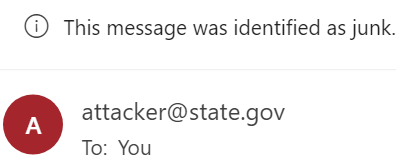
\includegraphics[clip,width=\columnwidth]{fig/ss_outlook_not_rejecting.png}}
}
    %\caption{Example message that has a spoofed FROM header using a domain with DMARC policy reject.  It is delivered to an Outlook user's spam folder instead of being rejected.}
    \vspace*{-0.2in}
    \caption{Example message with a FROM header spoofing a domain with DMARC policy \textsc{Reject}.  Outlook delivers it to the spam folder instead of rejecting it.
    }
    \label{fig:example_ms_not_rejecting}
    \end{figure}

%
% In our experiments, we find that four email providers (Outlook, Fastmail, GMX and Inbox.lv) follow this quarantine-over-reject approach.

Because these providers quarantine the spoofed email as spam, this
design does not appear particularly dangerous.\footnote{Some in the
  mail security industry criticize this weakening of DMARC
  rules and document attacks that ``rescue'' such email from the spam folder via social engineering~\cite{Microsof7:online,Spearphi83:online}.} However, as we
will show, in combination with email forwarding and another
vulnerable feature (per-user domain whitelists in Section~\ref{subsubsec:whitelist}), attackers can override this
protection and exploit the quarantine-over-reject implementation to spoof
email from thousands of popular domains despite their strict
DMARC \textsc{Reject} policy.

%In our work, we present new attacks that show how forwarding introduces a new avenue for exploiting this design.
%In particular, when combined with other vulnerable assumptions (e.g., Section~\ref{subsubsec:whitelist}), attackers can use forwarding accounts to override these quarantine protections and exploit the header rewriting changes in different forwarding approaches to spoof email messages from thousands of popular domains.
%Because of this quarantine-over-reject policy, these attacks are successful even when the spoofed domains have a strict DMARC policy of \textsc{Reject}.

% , and the resulting emails pass both SPF and DMARC validation at the recipient's mail server.

% there have been attacks that explotied this implementation decision as reported in prior blog posts~\cite{Microsof7:online,Spearphi83:online}.
%
% Even worse, as we detail below in Section~\ref{subsubsec:whitelist}, the quarantine decision can be overridden by a malicious user and thus creates a new threat to the downstream providers, potentially allowing an adversary to forward spoofed email messages even if the spoofed FROM domain has DMARC policy reject, endangering downstream providers. Indeed,
% we show in Section~\ref{subsec:attack_open_forwarding} that when an adversary combines such policies with email forwarding and other issues described in this section, they can often spoof email messages from a wide range of domains (even if these domains have DMARC policy reject) that correctly pass both SPF and DMARC validation at the recipient's mail server.

\subsubsection{Per-user DMARC overrides are fate-sharing}
\label{subsubsec:whitelist}
Many email providers allow users to override DMARC decisions: users can whitelist domains, and as a result they will still deliver or forward email even if it fails DMARC.
% \geoff{by ``upon a user's request'', do we just mean that users can whitelist domains to override DMARC?}\alex{yes, updated the text.}
Providers offer this flexibility because it can help mitigate
errors and improve mail deliverability for the users who need it.
However, this feature implicitly assumes that this approach is
fate-sharing --- that when a user overrides DMARC decisions, the risks
of that choice are localized to the individual user account.  While
true in the single-hop context, forwarding again undermines this
assumption.  If adversaries can override DMARC decisions on a
forwarding account they control, they can use that capability to
launder spoofed mail and successfully deliver it downstream.

 % While this can be convenient in certain use cases (e.g., to increase deliverability), it also allows an adversary to potentially forward spoofed email messages. When combined with \emph{open forwarding}, whitelisting enables an adversary to forward spoofed email messages to arbitrary destination, hurting the users of downstream providers and also invalidating the assumption that quarantining an email neutralizes the threat (Section~\ref{subsubsec:quarantine_instead_of_reject}) by introducing a new threat to downstream providers.

Based on our measurements, all mail providers support this functionality in some form.
Of particular note, four of the five providers 
mentioned in Section~\ref{subsubsec:quarantine_instead_of_reject}
(Fastmail, GMX, Inbox.lv, and Pobox)
allow users to override any DMARC decision for any domains.
The fifth (Outlook) allows users to override DMARC decisions for most domains, except for a small set of frequently-spoofed domains that have DMARC policy reject (e.g., \dns{aa.com}) where Outlook appears to apply additional, special protection mechanisms.

% We do not try to whitelist spoofed email messages at mailing list services as generally an adversary cannot have access to a mailing list's configuration. Mail2World.com does not enforce DMARC, so there is no need to override the decision. For the four providers mentioned in Section~\ref{subsubsec:quarantine_instead_of_reject} that do not reject any email, we can override DMARC decisions for all domains for three of them (Fastmail, GMX and Inbox.lv). We are able to override DMARC decision for most domains for Outlook, except for a small set of frequently-spoofed domains that have DMARC policy reject (e.g., \dns{aa.com}). We suspect Outlook has special protection mechanism for these domains.
For Gmail, Hushmail, iCloud, Mail.ru, Onet, and Zoho, users can override DMARC decisions for domains with DMARC policy \textsc{None} or \textsc{Quarantine}, but not \textsc{Reject}.  Finally, for Yahoo, we can only override DMARC decisions for domains with a policy of \textsc{None}.

% but place them in the spam folder instead of the inbox

 % should be rejected but instead delivered to spam.
% The spoofed FROM domain in this case is microsoft.com, which has DMARC policy reject.

% While this vulnerability does not seem to create huge security concerns, there has been reported attacks that exploited such vulnerability.



% Additionally, this vulnerability gives an adversary the ability to whitelist email messages that spoofed from domains with DAMRC reject. As can be seen from Section~\ref{subsec:attack_open_forwarding} and~\ref{subsec:attack_zoho_arc}, combining with other vulnerabilities, this enables an adversary to spoof from arbitrary domains.


 % simply preventing arbitrary FROM header forgery is not enough. A sophisticated adversary, who controls a personal account with third-party providers like Outlook, cam still abuse this shared infrastructure with the help of forwarding.


% \subsection{Assumptions Made in Practice}
\subsection{Vulnerable Forwarding Features}
\label{subsec:fwding_vuln}
In the absence of forwarding, the assumptions described above are
largely benign and allow the effective blocking of many spoofing
attacks.  However, when combined with three vulnerable forwarding
features, open forwarding, relaxed validation, and unsolicited DKIM signatures, the weaknesses in
these assumptions permit several opportunities for bypassing DMARC's
protections.

% and policies
%adopted by major email services that

%, when combined with the header rewriting during forwarding, enable attackers to violate and exploit the security assumptions discussed above.
% \grant{If we go with this structure, we'll need to think about how to word Table~\ref{tab:assumptions_and_prevalence}, or how to reword the vulnerable forwarding features/designs in this subsection.}

% \subsubsection{Users only forward to accounts they control}
% \subsubsection{Forwarding occurs benignly between accounts}
\subsubsection{Open Forwarding}
\label{subsubsec:open_forwarding}
% \alex{Open forwarding}
Many email service providers support a mechanism to automatically
forward a user's messages to another account (\eg, to aggregate mail
sent to multiple addresses into a single inbox).  Because of the
prevalence of these common, benign forwarding use cases, many
platforms follow a design that we call \emph{open forwarding} (also
referred to as ``unauthorized forwarding'' in previous work~\cite{shen2020weak}).  Services with open forwarding allow users
to configure their account to forward messages to any destination
email address, \textit{without} any verification from the destination
address.  Open forwarding implicitly assumes users will only forward
email to accounts that they control or have a benign relationship with
(an assumption that fails when an adversary creates or controls an account
entirely for the purpose of malicious forwarding).

%, which does not hold when adversaries create forwarding accounts for malicious purposes.

% This design decision implicitly assumes that users will only forward email to accounts that they control or have a benign relationship with, leading to an implementation decision which we term \emph{open forwarding} (also referred to as ``unauthorized forwarding'' in prior work~\cite{shen2020weak}) --- that no verification is performed against the destination address.

% Open forwarding implicitly assumes users will only forward email to accounts that they control or have a benign relationship with, which does not hold when adversaries create forwarding accounts for malicious porposes.
% However, this assumption does not hold reliably in the presence of adversaries. An adversary can create accounts and use it to
% redirect traffic to an arbitrary destination if no verification is performed.

Our measurements show that open forwarding is still prevalent among providers.
Specifically, ten email providers (Outlook, Fastmail, iCloud, Freemail, GoDaddy, Hushmail,
Mail2World, Onet, Pobox, and Runbox) allow open
forwarding.\footnote{Mail2World and Pobox do notify the destination account
via email about the forwarding setup.}  Moreover, as we demonstrate in three
attacks described in
Sections~\ref{subsec:attack_open_forwarding}--\ref{subsec:attack_zoho_arc},
%,~\ref{subsec:attack_relaxed_forwarding_validation},
%and~\ref{subsec:attack_zoho_arc},
when combined with other vulnerabilities, adversaries can exploit open
forwarding to attack not only users on those providers that employ
this design, but also a broad array of users on other platforms that
disallow open forwarding.
% can not only cause harm to users of the provider that allows it, but also affect the users of other providers.




\begin{table*}[t]
  \centering
  \begin{threeparttable}
  \small
  \begin{tabular}{p{0.08\textwidth}p{0.32\textwidth}p{0.3\textwidth}p{0.18\textwidth}}
    \toprule
  %  & \multicolumn{3}{c}{\textbf{Attacks}} \\
    & \textbf{Send email spoofing} & \textbf{Forward via} & \textbf{Deliver to} \\
    \midrule
   \multirow{2}{*}{\S~\ref{subsec:attack_open_forwarding}} & Domains with the forwarding domain's SPF information & Six providers including Outlook and iCloud & \multirow{2}{*}{Any recipient} \\
    & in their SPF records & & \\[1pt]
  \ltgrey
  & Arbitrary domains with DMARC policy None or Quarantine & Outlook & Gmail \\[1pt]
  \ltgrey
    \multirow{-2}{*}{\S~\ref{subsec:attack_relaxed_forwarding_validation}} & Arbitrary domains with DMARC policy None
    & Multiple providers (e.g., Fastmail)& Outlook \\[1pt]
    \S~\ref{subsec:attack_zoho_arc}\tnote{*} & Arbitrary domains & Fastmail & Zoho \\[1pt]
  \ltgrey
    & Domains hosting the mailing list and DMARC policy None & Google Groups, Listserv, Mailman & Any recipient \\
  \ltgrey
    \multirow{-2}{*}{\S~\ref{subsec:attack_none_mailing_list}} & Arbitrary domains & Gaggle & Any recipient \\
    \bottomrule
  \end{tabular}

  \begin{tablenotes}
  \item[*] We build on the ARC vulnerability
    identified by Shen et al.~\cite{shen2020weak}, to demonstrate an
    attack that is practical.
  \end{tablenotes}


  \end{threeparttable}
  \caption{Summary of email forwarding attacks (\S~\ref{sec:attacks}).
    \label{tab:summary_attacks}} 
%  \vspace*{-0.2in}

  \end{table*}



% \subsubsection{Large email providers' forwarding implementation can break DMARC, to allow forwarding to work, we can treat forwarded emails from them as benign}
\subsubsection{Relaxed Validation}
\label{subsubsec:relaxed_validation}
% \subsubsection{Forwarded emails from large providers can receive loosened validation}
% \alex{Relaxed Validation}
Since forwarded email can break SPF and DMARC at times, providers may employ relaxed validation for email forwarded by large email providers, assuming that these large providers will
% have good security hygiene and
prevent spoofed email messages from being forwarded.\footnote{Shen et al.~\cite{shen2020weak} also make this observation, but do not document the concrete steps necessary to exploit this vulnerability or demonstrate its practical exploitation.}

%  suggested such a possibility, but do not provide concrete details of how to exploit this vulnerability. \alex{quote \textbf{`because these
%emails are sent from a well-known email forwarding MTA,
%the receiver's MTA generally accepts such emails. '}}}

We infer that three providers, Gmail, Outlook and Mail.ru, apply some form of relaxed validation. Gmail employs two versions of relaxed validation for forwarded email messages that both (1) fail SPF and DMARC checks and (2) are from domains with a DMARC policy of \textsc{None} or \textsc{Quarantine}.
First, for email messages forwarded via Gmail or Outlook, Gmail delivers them regardless.
Second, for messages forwarded via
% other “well-known” providers (e.g., other providers in our experiments),
the other providers in our experiments,
Gmail delivers the email if it meets specific conditions (more details in Appendix~\ref{sec:append_change_behavior_details}).
% In both scenarios, besides delivering the email, Gmail would normally display a UI indicator to show that the email is forwarded. However, we observe a bug in the UI implementation --- sometimes a UI indicator is not displayed (Section~\ref{subsubsec:ui_bug}).

Similarly, our experiments found that Outlook applies relaxed validation for email messages from domains with a DMARC policy of \textsc{None}
%, except for a small set of high-profile ones
(as discussed in Section~\ref{subsubsec:dmarc_none}, Outlook usually overrides the policy of \textsc{None} and quarantines messages that fail DMARC).
Specifically, Outlook accepts email messages forwarded via nine major providers (e.g., Gmail and Fastmail),
%in our experiments,
despite failing SPF and DMARC checks.
Finally, Mail.ru accepts email messages forwarded via Gmail that fail DMARC from domains with a DMARC policy of \textsc{None} or \textsc{Quarantine}.
%For example, we observe that Gmail employs two versions of relaxed validation for forwarded email messages that (1) fail SPF and DMARC checks, and (2) are from domains with DMARC policy none or quarantine. For email messages forwarded via Gmail and Outlook, Gmail delivers them regardless. For email messages forwarded via other ``well-known'' providers (\eg, the other four providers in our experiments), Gmail delivers them as long as a specific condition is not met (more details in Appendix~\ref{sec:append_change_behavior_details})
%In both versions, besides delivering the email, Gmail would normally display a UI indicator to show that the email is forwarded. However, sometimes a UI indicator is not displayed due to a bug (Section~\ref{subsec:vul:ui_bug}).

%Similarly, Outlook uses relaxed validation for email messages from domains with DMARC policy none.  For instance,
%Outlook accepts email messages forwarded via any of the six email providers in our experiments, despite the fact they fail SPF and DMARC checks.

These relaxed validation policies aim to balance the incompatibility of forwarding approaches with anti-spoofing protocols by implicitly trusting high-profile email services.
Unfortunately, the complexity introduced by forwarding and its interactions with the diverse set of assumptions we highlight enable attackers to abuse these trust relationships.  This is particularly true because all of these providers offer individual consumer accounts.
% Such behavior creates an opportunity for an adversary to perform email spoofing attacks when the upstream forwarder supports \emph{open forwarding}, which allows an adversary to redirect spoofed email messages to arbitrary destination.
For example, in Section~\ref{subsec:attack_relaxed_forwarding_validation} we show that an adversary can deliver spoofed email messages from domains that have a DMARC policy of \textsc{None} or \textsc{Quarantine} to any Gmail user without triggering a warning.

\subsubsection{Unsolicited DKIM Signatures for Hosted Domains}
\label{subsubsec:unsolicited_dkim}
RFC 6376~\cite{rfc6376} and RFC 6377~\cite{rfc6377} both recommend that
forwarding services apply their own DKIM signatures for forwarded email
messages, especially for cases where they modify the message. 
Shen et al.~\cite{shen2020weak} showed that this configuration can be exploited
by a malicious actor via an attack that they called the DKIM Signature Fraud
Attack.  Specifically, they showed that an adversary can acquire valid DKIM
signatures for spoofed email messages if the forwarder naively signs every
forwarded email. Such spoofed email messages can successfully pass subsequent
DMARC checks if their spoofed sender's domain is the same as the domain used by
the forwarding service to sign DKIM signatures. Shen et al.~\cite{shen2020weak}
found three providers that had this vulnerable feature: Yahoo, Office365 and
Alibaba Cloud.
% Readers are referred to Shen et al.~\cite{shen2020weak} for more details on
% the DKIM Signature Fraud Attack.

Through our experiments, we identified that three providers' (iCloud, Hushmail, and Runbox) forwarding implementation contained a variant of this vulnerable feature, which would allow an adversary to mount attacks similar to the DKIM Signature Fraud Attack.
Taking iCloud as an example, we find that iCloud adds unsolicited and valid DKIM signatures to spoofed email messages addressed from domains hosted by them. Additionally,
iCloud signs the DKIM signature using the same domain as the purported sender's domain in the spoofed email. For instance, iCloud will add a valid DKIM signature signed by the domain \texttt{peterborgapps.com} (a domain hosted by iCloud) to spoofed email messages purporting to be from \texttt{peterborgapps.com}, allowing the spoofed email messages to pass subsequent DMARC checks.
We surmise that providers can add valid DKIM signatures on behalf of hosted domains because they manage DKIM keys for these domains~\cite{Setupane66:online, HushDKIM}.



% Similarly, an adversary could spoof email messages from domains with DMARC none to any Outlook user.
% In contrast, if an email message is directly sent to Outlook and fails DMARC checks, it will be quarantined (as noted in Section~\ref{subsubsec:dmarc_none}).


%% \subsubsection{Forwarded email messages do not have spoofed identity}
%% % \alex{I kinda think this is not necessary/a thing, but not sure. Dump the text here just in case and leave it to Stefan/Geoff}
%% % \grant{Hmmm... I'm not really convinced by the content in this subsection. The examples here don't really resonate with me, but maybe I'm missing something?}
%% \grant{Per meeting: Marking this as a section to cut unless someone sees a good reframing.}
%% All forwarding mechanisms to some extent assume that the Mailfrom header and / or the From header are not spoofed. For example, PMF forwards the message faithfully by preserving both the Mailfrom header and the From header. This can cause problems if an adversary is somehow able to force the forwarding of an email that has spoofed headers, letting the adversary abuse the lying functionality of forwarding. Similarly, REM always rewrites the Mailfrom header be an address in the forwarding domain, which introduces issues when the From domain is spoofed to be same as the forwarding domain (noted by Shen et al.~\cite{shen2020weak}).

%\subsection{Measuring Assumption Violations in the Wild}
%\label{subsec:measure_assumptions}
%\alex{The mapping between assumption and implementation is a bit unclear to me}

% To understand what attacks an adversary could perform, one first has to understand what vulnerabilities exist in the email forwarding flow. We measure/explore vulnerabilities that exist in email forwarding flow by testing the system with legitimate emails and emails that have spoofed FROM headers. Table~\ref{tab:summary_indi_vulnerabilities} lists vulnerabilities observed at each party in the forwarding flow.

% \begin{figure}[htbp]
% \centerline{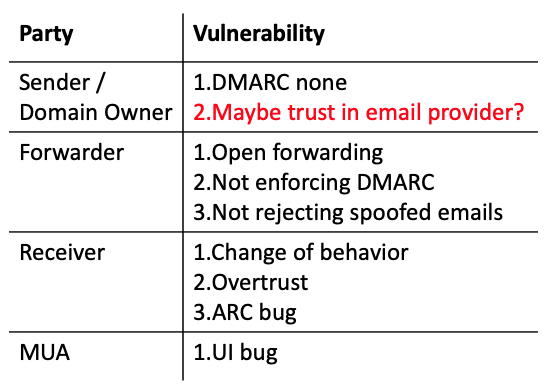
\includegraphics[width=\columnwidth]{graphs/summary_indi_vulnerabilities.png}}
% \centering
% \caption{Summary of Vulnerabilities Identified}
% \label{fig:summary_indi_vulnerabilities}
% \end{figure}

% Please add the following required packages to your document preamble:
% \usepackage{multirow}



% \subsection{Implementation Errors}
% \label{subsec:implementation_errors}
% Finally, in addition to vulnerabilities
% resulting from the design of forwarding and anti-spoofing mechanisms,
% during our experiments we also observed three implementation
% errors. We focus on Zoho's ARC implementation error, which directly
% introduces serious security concerns. The other two errors can be
% abused to help send spoofed email, which we detail in
% Appendix~\ref{sec:implementation_errors_additional}.


% in a subset of our attacks.
% Namely, Gmail's UI indicator bug and Zoho's ARC implementation bug.

% \subsubsection{Every email is legitimate}
% \grant{Hmmm... this subsection really strikes me as a broken implementation, and we might consider moving to Section 4.2}


% \subsubsection*{Zoho's ARC Implementation Error}
% \label{sec:arc}
% % \label{subsubsec:arc_bug}
% As discussed earlier in Section~\ref{sec:measure_forwarding_mechs_and_arc},
% many forwarding approaches break SPF, DKIM, and DMARC authentication.
% To remedy this compatibility issue, a new experimental protocol called Authenticated Received Chain (ARC)~\cite{rfc8617} was recently introduced to preserve email authentication results across multiple forwarders and allow the final recipient to authenticate legitimate email even if they fail DMARC authentication.
% Intermediary forwarders implementing ARC sign their authentication results
% (using new ARC headers) so that the receiver can verify each forwarder's authentication checks.
% If DMARC authentication fails, a receiver can examine the ARC validation chain to determine whether the forwarded email is legitimate~\cite{ARCSpeci1:online}.
% Although ARC can help resolve the compatibility issues with some forwarding implementations and anti-spoofing protocols, it does not remedy the security vulnerabilities presented earlier in this section.
% Additionally, ARC is currently an experimental standard and only
% implemented by a few providers~\cite{rfc8617, ARCSpeci1:online};
% Appendix~\ref{sec:appendix_arc_measurement}
% % and Table~\ref{tab:forwarding_mechs_in_the_wild}
% reports our measurement results about the adoption of ARC among
% the providers we evaluated.
% %\geoff{(will need to be updated if ARC is removed from the table)}
% Nonetheless, during our experiments, we identified attacks that can exploit incorrect ARC implementations to reliably spoof email.

% Among these platforms, many providers only accept ARC signatures from custom lists of ``trusted'' forwarders (Table~\ref{tab:trust_of_arc_between_providers}).
% During our analysis, we discovered that some email providers' implementation of ARC also leads to vulnerabilities, which an attacker can combine with forwarding to spoof malicious emails (\S~\ref{subsec:attack_zoho_arc}).
% Prior work has found that some mail providers, such as Zoho, incorrectly implement ARC~\cite{shen2020weak}.
% For example, when a spoofed email message is forwarded from Gmail to Zoho, Zoho incorrectly reads the ARC headers attached by Gmail. As a result, it incorrectly displays the email as passing DMARC and delivers the email without warnings.
% Echoing this prior work, we found that this vulnerability still existed at Zoho.
% We also found through our experiments that, in addition to Gmail, Zoho also evaluates and trusts ARC headers added by Fastmail (Section~\ref{sec:measure_forwarding_mechs_and_arc}).
% Moreover, by leveraging Fastmail's open forwarding, this flawed ARC implementation could be exploited to spoof email messages to any Zoho user from \emph{any} domain.\footnote{Our work not only led to a patch of this issue after disclosure to Zoho, but also resulted in Zoho adding additional security enhancements to their ARC implementation (Appendix~\ref{sec:disclosure}).  This patch is confirmed by the parallel work of Wang et al.~\cite{wang2022revisiting} that focused on email forwarding under ARC.}


%% \begin{figure}[t]
%%   \centering
%%   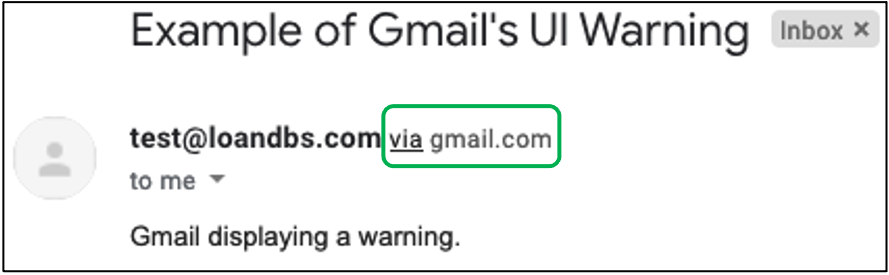
\includegraphics[width=\columnwidth]{graphs/ss_ui_warning_normal.png}
%%   \caption{Gmail's usual UI warning for forwarded mail.}
%%   \vspace*{-0.1in}
%%   \label{fig:gmail_ui_normal}
%% \end{figure}

% However, any such trust implicitly
% assumes that those trusted forwarders have good security practices.
% Unfortunately, as we detail later, this is not always the case, which
% creates additional opportunities for adversaries
% (Section~\ref{subsec:attack_zoho_arc}).


%
% attack summary table in previous section for positioning
%

\section{Attacks}
\label{sec:attacks}
In this section, we demonstrate how an adversary can combine and
exploit the issues
% we have
described in Section~\ref{sec:assumptions} to create attacks that reliably
bypass existing anti-spoofing protections.  In particular, we consider an
attack successful if a spoofed email message is delivered to a
victim's inbox (\ie,  not the spam folder), and yet does not produce a
warning to the user.
Figure~\ref{fig:open_forwarding_attack_screenshot} shows
an example of a successful attack, where a spoofed
email purporting to be from \dns{bush@state.gov} is delivered to a
Gmail user's inbox with no warning indication.

We describe four distinct classes of attacks, summarized in
Table~\ref{tab:summary_attacks}, each of which we have validated
empirically using accounts created at the affected providers.  Some of
these attacks are quite broad --- allowing an attacker to spoof email
to any email recipient purporting to be from tens of thousands of
popular and sensitive domains --- while others are more circumscribed
in their impact.
%
For each of the attacks described below, we refer to the domain an
attacker specifies in their \textsc{FROM} header as the
\textit{spoofed domain}.  We use the terms \textit{spoofed address} to
refer to the full email address appearing in the \textsc{FROM} header
and \textit{forwarding domain} to refer to the domain of the
forwarder.

\begin{figure}[t]
  \centering
%% \centerline{
\includegraphics[width=\columnwidth]{graphs/ss_outlook_open_forwarding.png}}
{
    \setlength{\fboxsep}{0pt}
    \setlength{\fboxrule}{0.5pt}
    \fbox{
\includegraphics[trim=2 2 2 47,clip,width=\columnwidth]{fig/ss_outlook_open_forwarding.png}}
}
%  \vspace*{-0.2in}
  \caption{Example of a successful attack. A spoofed email purporting to be \dns{bush@state.gov} is delivered to a Gmail user's inbox with no warning indicators.
}
%\vspace*{-0.1in}
\label{fig:open_forwarding_attack_screenshot}
\end{figure}


\begin{figure*}[t]
  \centerline{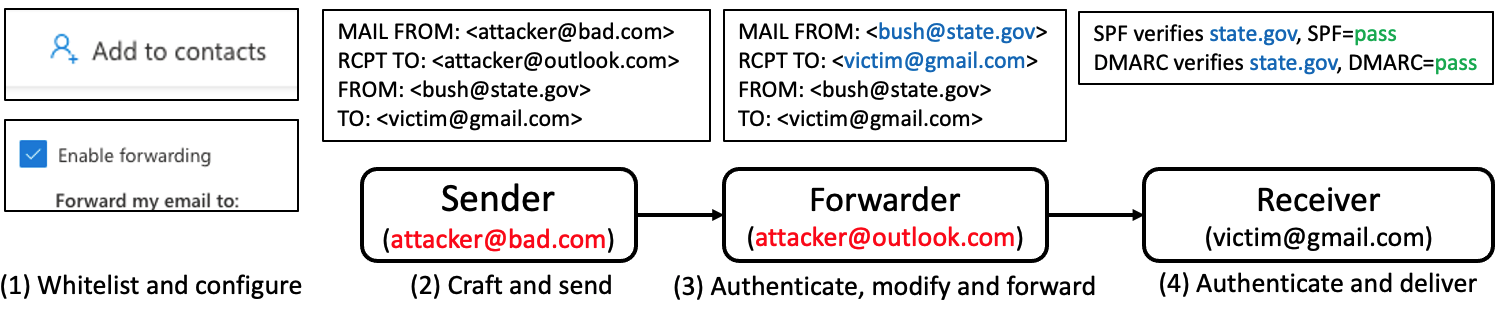
\includegraphics[width=\textwidth]{fig/mech_outlook_open_forwarding.pdf}}
  \centering
  \caption{Example of an SPF Incorporation Attack (\S~\ref{subsec:attack_open_forwarding}) exploiting Outlook's open forwarding to spoof email from domains incorporating Outlook's SPF records (e.g., \dns{state.gov}) to arbitrary recipients.}
  \label{fig:open_forwarding_attack_mechanism}
  %    \vspace*{-0.1in}
\end{figure*}


\paragraph{Threat Models}
For the first three attacks, we assume an adversary controls the
sender and forwarding accounts: they possess a server capable of
sending spoofed email messages (sender) and a personal account with a
specific third-party provider that allows \emph{open forwarding}
(forwarder). For the attack described in
Section~\ref{subsec:attack_none_mailing_list}, we make three
assumptions: (a) that adversaries control a malicious server that can
send spoofed email messages and try to spoof email from a domain that
hosts a mailing list with REM forwarding (e.g., Google Groups,
Listserv and Mailman as described in
Section~\ref{sec:measure_forwarding_mechs_and_arc}), (b) that the spoofed domain
has a DMARC policy of \textsc{None} (all too common); and (c) the
sending email address the attacker wishes to impersonate has
permission to send to the mailing list.

%We validated each of these attacks empirically using
%accounts we created with each of the affected providers.
%Additionally, we have disclosed all of these vulnerabilities to the
%affected providers (Section~\ref{sec:disclosure}).

%We also demonstrate how an adversary can ``launder'' spoofed email
%through mailing lists, such that the resulting spoofed email also
%passes SPF and DMARC validation checks.


%% include email addressed from: (1) any
%% domain that incorporates Outlook's SPF information in their SPF
%% records (\ie, including thousands of high-profile domains such as
%% \dns{state.gov}, \dns{disneyplus.com}, and \dns{qantas.com}),\alex{do we still want to say any domain} (2) any
%% domain, if the recipient is a Zoho user, and (3) any domain with a
%% DMARC policy of none or quarantine (\eg, \dns{alipay.com}), if the
%% recipient is a Gmail user.

%\grant{I'm not sure how I feel about the caveats about specific email provider. They seem to detract / complicate the impact examples and I wonder if others feel the same or see a way to word them more broadly (e.g., in terms of forwarding approaches, rather than specific providers).}
%\geoff{since we have even more qualifiers on the attacks than before (e.g., Alex's note about any domain no longer being accurate), how about if we reduce this part to something on the order of ``in some cases impacting ....''}

% For the remainder of this section, we
% describe each of these attacks in detail and explain what enables each
% to bypass existing anti-spoofing measures.

%Each attack combines vulnerable forwarding features (\S~\ref{subsec:fwding_vuln}) and/or the header rewriting performed by common forwarding approaches (\S~\ref{sec:background:fwdingflow}) to violate security assumptions made by anti-spoofing defenses (\S~\ref{subsec:assumptions}).
%While these defenses would have mitigated spoofing in a direct email transmission settings, the use of forwarding enables successful spoofing attacks.
% For each attack, we describe the steps an attacker performs to successfully spoof an email and explain how forwarding,
% combined with the vulnerabilities from Section~\ref{sec:assumptions} enable the attack to bypass anti-spoofing measures.
 % and will report on their feedback in a final version of this paper.

% In all four attacks, we assume that the adversary controls their own SMTP server for sending spoofed email messages (i.e., the sender is malicious). Additionally, for the first three attacks, we assume that the adversary also controls personal email accounts registered with the forwarder, which is easily done with services like Outlook and Fastmail. For the last attack involving mailing lists, we assume that the adversary knows a target email address within the organization that is allowed to send to the mailing list.


\begin{figure*}[t]
  \centerline{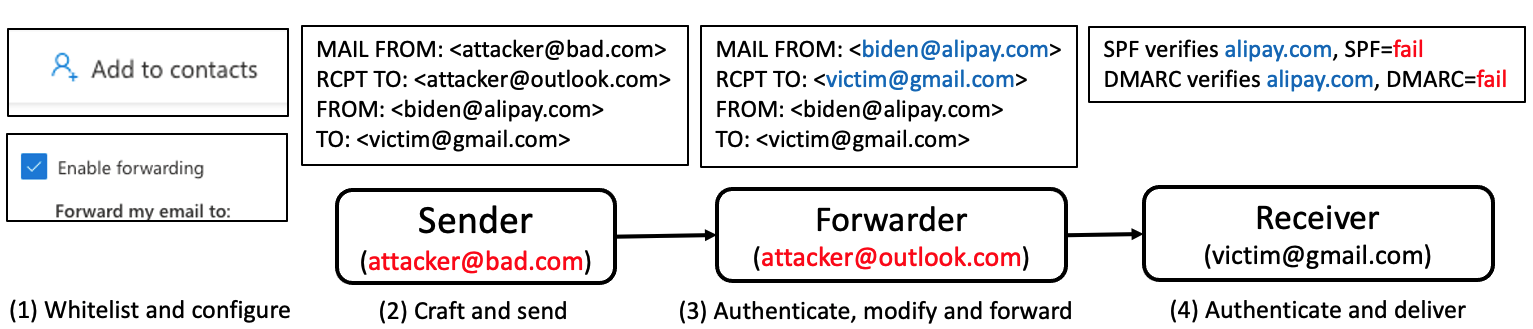
\includegraphics[width=\textwidth]{fig/mech_gmail_via_outlook.pdf}}
  \centering
  \caption{Example of a spoofed email attack exploiting open forwarding and relaxed validation for forwarded email from well-known providers (\S~\ref{subsec:attack_relaxed_forwarding_validation}).
    Note that the spoofed domain, \dns{alipay.com}, has a DMARC policy of Quarantine and thus
    % its traffic
    should not be delivered.}
  \label{fig:mech_gmail_via_outlook}
\end{figure*}


\subsection{Exploiting SPF Incorporation}
\label{subsec:attack_open_forwarding}

% \subsubsection*{Attack Overview}
The first attack we describe exploits five discrete issues:
three security assumptions (\S~\ref{subsubsec:spf_incorporation},~\ref{subsubsec:quarantine_instead_of_reject},~\ref{subsubsec:whitelist}),
the vulnerable \emph{open forwarding} feature that many providers offer (\S~\ref{subsubsec:open_forwarding}),
and the header rewriting performed as part of the PMF and MFEF forwarding approaches (\S~\ref{sec:measure_forwarding_mechs_and_arc}).
Crucially,
%as described in Section~\ref{subsubsec:spf_incorporation},
the rise of large third-party email providers violates SPF's assumption that the set of authorized server IP addresses specified by each domain cannot be used by other domains or external users to send email.
% SPF assumes that set of authentic server IP addresses that each domain specifies cannot be used by other domains or external users to send emails. The rise of third-party providers has challenged this assumption --- many domains now outsource their email services to these third-party email providers.
For example, the owners of domain \dns{state.gov} use Outlook as their email provider.  Thus, email messages sent by \dns{state.gov}'s employees will originate from Outlook's mail servers.
To ensure reliable delivery, such domains routinely add the server IP addresses of their email provider to their own SPF records.
Although intuitive, this configuration creates an overly broad trust assumption: by adding the provider IP addresses to their SPF record, such domains (e.g., \dns{state.gov}) implicitly grant permission for any account hosted by their provider, whether individual or corporate, to send email messages that purportedly come from their domain.
This threat is only prevented because large providers like Outlook do not allow users to arbitrarily set or forge their email's FROM header.

However, we observe that by combining header rewriting from PMF and MFEF and the use of \emph{open forwarding}, attackers can overcome this defense and exploit SPF's violated assumption.
Specifically, this attack allows an adversary to spoof email from domains that incorporate a third-party provider's SPF information in their own SPF record to any recipient, regardless of the domain's DMARC policy.
%absent additional protections.

% Outlook also enables \emph{open forwarding} and uses the MFEF forwarding approach, which provides attackers with a mechanism for sending email messages with forged FROM headers.
% While Microsoft does not provide a mechanism for forging the FROM header, a malicious sender can spoof as arbitrary domain in the FROM header. With open forwarding, an adversary can create an individual Outlook account and use it to redirect an email with a forged FROM header to an arbitrary destination without verification.
% Together, these issues allow an adversary to reliably spoof as any domain that incorporates a third-party provider's SPF information in their own SPF absent some other protection.
% \subsubsection*{Impact}
%\paragraph{Impact}
\paragraph{Scope}
This attack works for domains that include the SPF record of any of six
large email providers (Outlook, iCloud, Freemail, Hushmail, Mail2World and Runbox) in their own SPF records.  Notably, given
Outlook's importance as a third-party provider~\cite{liu2021s}, this
attack allows an attacker to spoof email on behalf of tens of
thousands of popular domains.

Indeed, over 12\% of the Alexa 100K
most popular domains are vulnerable as a result (and almost 8\% of the
top 1M domains).  A cursory examination of this list identified a
range of potentially sensitive domains such as those hosting large
news reporting organizations (\eg, \dns{washingtonpost.com},
%\dns{cbsnews.com},
\dns{latimes.com},
%\dns{slate.com}, \dns{npr.org},
and \dns{apnews.com}),
%\dns{nydailynews.com} and \dns{afp.com}),
financial services (\eg,
%\dns{usbank.com}, \dns{discover.com},
\dns{mastercard.com}, \dns{transunion.com},
%\dns{fidelity.com},
and \dns{docusign.com}),
domain registrars (\eg, \dns{godaddy.com}),
certificate authorities (\eg,
\dns{sectigo.com} and \dns{digicert.com}) and large law firms (\eg,
\dns{perkinscoie.com}).  In addition, 32\% of US \dns{.gov} domains are
vulnerable (including 22\% of the domains used by Federal
agencies).  At the Federal level this includes the majority of US
cabinet organizations (\eg, \dns{state.gov}, \dns{dhs.gov} and
\dns{doe.gov}), a range of security sensitive agencies (\eg,
\dns{odni.gov}, \dns{cisa.gov} and \dns{secretservice.gov}) as well
as those charged with public health and safety (such as
\dns{fema.gov}, \dns{nih.gov}, and \dns{cdc.gov}).
%% \footnote{To say
%%   nothing of other critical government functions such as the funding
%%   of scientific research (\eg  nsf.gov).}
At the state and local
level, virtually all primary state government domains (\eg, \dns{mass.gov})
  are vulnerable (including a broad range of congress, judiciary,
  and law enforcement domains in each state) and over 40\% of all \dns{.gov}
  domains used by cities.\footnote{We have not broadly examined domains representing government offices outside the US, but we note that both \dnsfn{gchq.gov.uk} and \dnsfn{ncsc.gov.uk} are also vulnerable.}


% \footnote{Our estimation suggests that roughly
% 12.4\% of Alexa top $100K$ domains and 38.1\% of \dns{.gov} domains are
% vulnerable to this attack absent some other protection
% mechanism.
% This list includes both popular commercial domains such as \dns{disneyplus.com},  \dns{hulu.com} and \dns{qantas.com} and sensitive domains used by the U.S. government in its official capacity such as \dns{state.gov}, \dns{nsf.gov}, \dns{cdc.gov} and \dns{cisa.gov} among many others.}.


%% %Absent additional per-domain protections by
%% %Outlook(\S~\ref{subsubsec:whitelist}), this attack can be used to spoof any domain that incorporates Outlook's SPF information in their SPF
%% %record, regardless of the domain's DMARC settings (e.g., even with a
%% %policy of Reject).  Additionally, they can successfully deliver this
%% %spoofed email to any recipient at any email provider.
%% %\geoff{revisit: qualify this slightly in light of aa.com}
%% %
%% Figure~\ref{fig:open_forwarding_attack_mechanism} shows an example of
%% this attack using Outlook as the forwarding service. It consists of four stages.
%% %\label{subsubsec:open_forwarding_attack_mechanism}
%% %\alex{Updated the text}\grant{Would it work to incorporate this email forging as part of Stage 1,
%% %perhaps even just as text (Without changing the diagram).
%% %It's a little weird that we list some actions the attacker needs to do, and then talk about ``Stage 1'' and what the attacker does.}
%% An attacker starts by creating a personal account for
%% forwarding (\dns{attacker@outlook.com}), adding the spoofed address
%% (\dns{bush@state.gov}) to the account's ``allowlist'' (thereby
%% preventing any quarantining by Outlook), and configuring the account to
%% forward all email to the desired target (\dns{victim@gmail.com}). In this case, the spoofed domain \dns{state.gov} includes
%% Outlook's SPF record (\dns{spf.protection.outlook.com}) into its own SPF record and has a DMARC policy of \textsc{Reject}. Next, the attacker forges an email that purportedly originates from \dns{state.gov} and sends it to their personal Outlook account. Then, even though the message fails DMARC validation, Outlook will still forward it because the spoofed address is present in the account's allowlist.

  
  
% \subsubsection*{Threat Model and Attack Procedure}
%\paragraph{Attack Procedure}
\paragraph{Example}
%% \alex{another version of the above paragraph that works in the assumptions.}
% (need to reference the figure somewhere)
Figure~\ref{fig:open_forwarding_attack_mechanism} shows an example of
this attack using Outlook as the forwarding service.
An attacker starts by creating a personal account for
forwarding (\dns{attacker@outlook.com}), adding the spoofed address
(\dns{bush@state.gov}) to the account's ``allowlist'' (thereby
preventing any quarantining by Outlook), and configuring the account to
forward all email to the desired target (\dns{victim@gmail.com}). In this case, the spoofed domain \dns{state.gov} includes
Outlook's SPF record (\dns{spf.protection.outlook.com}) into its own SPF record and has a DMARC policy of \textsc{Reject}. Next, the attacker forges an email that purportedly originates from \dns{state.gov} and sends it to their personal Outlook account. Normally, Outlook would quarantine this email because it fails DMARC validation (\S~\ref{subsubsec:quarantine_instead_of_reject}). However, since the spoofed address is present in the account's allowlist, this configuration overwrites the quarantine decision (\S~\ref{subsubsec:whitelist}), and as a result, Outlook would forward the spoofed email to the target.


As per Outlook's MFEF forwarding implementation,
%the
\textsc{MAIL FROM}
%header
is rewritten to match the
\textsc{FROM} header, \dns{bush@state.gov} in our example. Finally, the recipient's mail server receives the forwarded email
and performs authentication checks.
From the recipient's perspective,
the spoofed email passes SPF validation because the
\textsc{MAIL FROM} domain (\dns{state.gov}) lists Outlook's SPF
information in its SPF record, and the forwarding configuration
arranged by the attacker ensures that the recipient receives this
spoofed email from Outlook's servers.
Moreover, this attack also
ensures that DMARC's alignment check succeeds because the
\textsc{MAIL FROM} and \textsc{FROM} domain are both \dns{state.gov}.
%\stefan{I don't think we need the screenshot.  I think they will believe us}
%\alex{nope we need this one}
We validated this attack in practice, consistently sending
spoofed email messages such as the example
shown in Figure~\ref{fig:open_forwarding_attack_screenshot}
to our own Gmail account, where it was delivered to the inbox without warning.\footnote{
Note that we did discover some exceptions in our experiments.
For a small set of high-profile domains that have a DMARC policy of Reject
(\eg, \dnsfn{aa.com}, \dnsfn{foxnews.com} and \dnsfn{ikea.com}), Outlook would
quarantine spoofed email regardless of whether users have added the
spoofed address to their account's allowlist (Section~\ref{subsubsec:quarantine_instead_of_reject}).
We surmise that Outlook applies special protections for a set of high-profile or frequently spoofed domains.
} 
In addition to Outlook, this attack also succeeds with
% five other large email providers:
iCloud, Freemail, Hushmail, Mail2World and Runbox.


\subsection{Abusing Relaxed Forwarding Validation}
\label{subsec:attack_relaxed_forwarding_validation}

% \subsubsection*{Attack Overview}
The second attack exploits the fact that many email providers apply relaxed validation policies to forwarded mail (\S~\ref{subsubsec:relaxed_validation}), particularly when messages arrive from well-known mail providers.
When combined with open forwarding, an attacker can abuse this behavior
to spoof email from any domain that has a DMARC policy of
%\geoff{is an and valid here?}\alex{yes. for gmail it is None and Quarantine}
\textsc{Quarantine} (or \textsc{None}) to any mail server that applies these relaxed measures (\eg, Gmail and Outlook).  Recall that, in the absence of forwarding, attackers cannot spoof email from a domain with a DMARC policy of \textsc{Quarantine}.
Provider-specific defenses, such as when Outlook quarantines any email that fails DMARC (\S~\ref{subsubsec:dmarc_none}), will also stop such direct, single-hop attacks.

\begin{figure*}[t]
\centerline{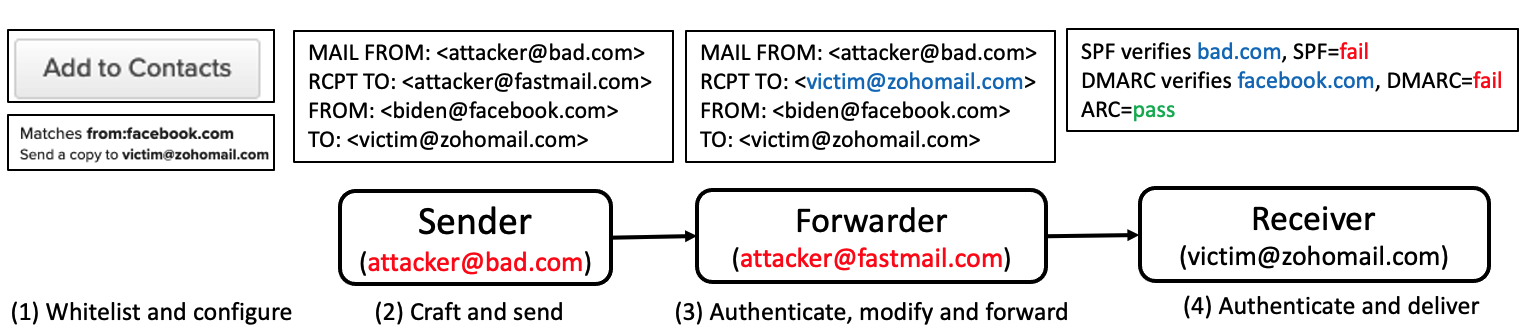
\includegraphics[width=\textwidth]{fig/mech_zoho_arc.pdf}}
\centering
\caption{Example attack that exploits Zoho's
vulnerable ARC implementation and  open forwarding to
  spoof email from arbitrary domains to any Zoho recipient (\S~\ref{subsec:attack_zoho_arc}).}
\label{fig:mech_zoho_arc}
%\vspace*{-0.1in}
\end{figure*}

% \subsubsection*{Impact}
%\paragraph{Impact}
\paragraph{Scope}
As described earlier in Section~\ref{subsubsec:relaxed_validation}, Gmail and Outlook use relaxed validation checks for forwarded email.
We find that an adversary can mount this attack against users with
Gmail/Outlook email accounts as well as users who use GSuite and Outlook 365 for email services.\footnote{Mail.ru also uses relaxed validation, but since it is only applied to email forwarded via Gmail, which does not allow open forwarding, this attack does not work for Mail.ru.}
%As a result, this attack impacts
% who together have
% roughly 1.9 billion users worldwide~\cite{GmailWik42:online, Outlookc33:online}
% when taking into account both users with
% Gmail/Outlook email accounts, as well as all users who use GSuite and
% Outlook 365 for email services (who are also vulnerable)

% \subsubsection*{Threat Model and Attack Procedure}
%\paragraph{Attack Procedure}
\paragraph{Example}
Figure~\ref{fig:mech_gmail_via_outlook} illustrates the steps of this
attack using an example where the adversary creates a personal Outlook
account to forward spoofed email messages to Gmail recipients.  First,
the adversary selects a spoofed email address from a domain with a
DMARC policy of \textsc{Quarantine} or \textsc{None} (we use \dns{alipay.com} in this example, a prominent Chinese payment company), adds the address
to their forwarding account's allowlist, and configures their
forwarding account to send email to the victim (recipient).  Like the
first attack, the attacker then sends a message from this spoofed address
to their forwarding account, which is then forwarded to the recipient.

When the final recipient's mail server receives
the email, the server will observe that the email comes from a
``well-known'' provider, apply its relaxed validation checks, and
successfully deliver the email to the recipient's inbox (even though
the spoofed email fails normal SPF and DMARC checks).\footnote{Additionally, we note that Gmail would usually display a UI warning for forwarded email messages. However, no UI warning is displayed for this email due to a bug detailed in Appendix~\ref{subsec:ui_bug}.}
%\alex{The part that talks about the UI bug}
%We verified this attack, and Figure~\ref{fig:ss_gmail_via_outlook} in the Appendix shows one such spoofed message delivered to GMail without security warnings.


\subsection{Targeting ARC Vulnerabilities}
\label{subsec:attack_zoho_arc}
% \subsubsection*{Attack Overview}
The third attack allows an adversary to deliver spoofed email messages
from arbitrary domains to Zoho users.  This attack exploits Zoho's
vulnerable implementation of the experimental Authenticated Received
Chain (ARC) protocol~\cite{ARCSpeci1:online}, which was first
documented by Shen et al.~\cite{shen2020weak}. Due to this bug, Zoho
incorrectly reads ARC headers and will deliver arbitrary email
messages with ARC headers added by providers such as Gmail and
Fastmail to the recipient's inbox without any warning.  However, we
show that this issue is not limited to interactions between Gmail and
Zoho customers.  We demonstrate how further issues, including the fact that
Zoho trusts and (incorrectly) reads ARC headers added by Fastmail
(Appendix~\ref{sec:arc_adoption_and_trust}), open forwarding
(\S~\ref{subsubsec:open_forwarding}), and several forwarding
assumptions (\S~\ref{subsubsec:quarantine_instead_of_reject},
\S~\ref{subsubsec:whitelist}), can be combined with the underlying ARC
vulnerability to allow an adversary to deliver spoofed email messages
from arbitrary domains to arbitrary Zoho users.

This attack again highlights the fact that email security protocols
are distributed and independently-configured components, where
vulnerable decisions by one party incur harm to downstream recipients
but not necessarily to their own users.  Notably, the actions taken
by one provider (e.g., Fastmail) can unexpectedly undermine the
security of users on another platform (e.g., Zoho).

%This attack works by combining several vulnerabilities: Zoho's vulnerable ARC implementation (more details below), 

%One main vulnerability exploited in this attack is Zoho's vulnerable
%implementation of the experimental Authenticated Received Chain (ARC)
%protocol~\cite{ARCSpeci1:online}, which was first documented by Shen
%et al.~\cite{shen2020weak}. Due to this bug, Zoho incorrectly reads
%ARC headers and will deliver arbitrary email messages with ARC headers
%added by providers such as Gmail and Fastmail to the recipient's inbox
%without any warning.

%To make this attack work, an adversary needs to
%exploit multiple different vulnerable forwarding assumptions and
%features, in addition to the flaw in Zoho's ARC implementation.
%We note that our work has not only led
%to a patch resolving this issue after disclosure to Zoho, but also
%resulted in Zoho adding additional security enhancements to their ARC
%implementation (Section~\ref{sec:disclosure}).
%\stefan{
%\grant{I'm commenting out the list of vulnerable things below because it seems redundant with both the intro paragraph and the attack description.}

% Importantly, several forwarding assumptions and open forwarding are required for this attack to work, in addition to Zoho's buggy ARC implementation. Namely, the attack we demonstrate in this section exploits that Fastmail allows open forwarding (Section~\ref{subsubsec:open_forwarding}), that Fastmail allow users to overwrite DMARC decisions through whitelisting (Section ~\ref{subsubsec:whitelist}), that Fastmail does not reject spoofed email messages addressed from domains with DMARC policy \textsc{REJECT} (Section~\ref{subsubsec:quarantine_instead_of_reject}), and that Zoho (incorrectly) reads ARC headers added by Fastmail (Appendix~\ref{sec:appendix_arc_measurement}). We provide more details in the example below.

%\paragraph{Impact}
\paragraph{Scope}
Our experiments show that this attack can target arbitrary users of Zoho, which is estimated to have more than 10 million users~\cite{Celebrat69:online}.

 % To some estimate~\cite{Celebrat69:online}, this attack impacts more than 10 million users.

%% \begin{figure}[t]
%% \centering
%% \includegraphics[width=\columnwidth]{graphs/mech_google_groups.pdf}
%% \centering
%% \caption{Spoofed email attack that abuses mailing lists like Google Groups (\S~\ref{subsec:attack_none_mailing_list}).}
%% \label{fig:google_groups_mech}
%% \vspace*{-0.1in}
%% \end{figure}

%% (geoff: since we have extra space in the camera ready version, I
%% resized this figure so that its elements are roughly the same size
%% as the first three attack figures.  feel free to undo if you don't
%% like it)
\begin{figure*}[t]
\centering
\includegraphics[width=\textwidth]{fig/mech_google_groups.pdf}
\centering
\caption{Spoofed email attack that abuses mailing lists like Google Groups (\S~\ref{subsec:attack_none_mailing_list}).}
\label{fig:google_groups_mech}
%\vspace*{-0.1in}
\end{figure*}




% \subsubsection*{Threat Model and Attack Procedure}
%\paragraph{Attack Procedure}
\paragraph{Example}
Figure~\ref{fig:mech_zoho_arc} shows the mechanics of this attack
%,
%which also consists of four phases,
in the context of an attacker with a forwarding account on Fastmail who targets a recipient on Zoho.

First,
%, as in the first attack,
the adversary creates a Fastmail account for forwarding, adds their spoofed address
(\dns{biden@facebook.com}) to their allowlist, and configures their
account to forward all mail to the target user at Zoho
(\dns{victim@zohomail.com}).
Second, the adversary crafts and sends
spoofed email from their own servers (\eg, \dns{attacker@bad.com})
to their forwarding account at Fastmail.
Third, although this email will fail anti-spoofing validation, Fastmail will still faithfully forward it to the target user at Zoho due to the sender's presence on the user's allowlist (exploiting the security assumption discussed in \S~\ref{subsubsec:whitelist}). 
As part of the forwarding process,
Fastmail will modify the RCPT TO header and add corresponding ARC headers to the
spoofed email.
Finally, upon receiving the forwarded email, Zoho's mail server will perform DMARC validation.
Although the spoofed email will fail SPF and DMARC checks,
Zoho's vulnerable ARC implementation
will misinterpret the ARC headers that Fastmail attached (Appendix~\ref{sec:arc_adoption_and_trust}).
As a result, Zoho will treat the email as passing
DMARC and deliver the spoofed message to the victim's inbox. We end by noting that this attack would not have worked for domains with DMARC policy \textsc{Reject} had Fastmail rejected spoofed email messages addressed from such domains (\S~\ref{subsubsec:quarantine_instead_of_reject}).
%Figure~\ref{fig:ss_zoho_arc} in the Appendix illustrates that this attack succeeds without any security warnings, even though the spoofed domain in our experiment, facebook.com, has a DMARC policy of \textsc{reject}. 

% \begin{figure}[t]
%   \centerline{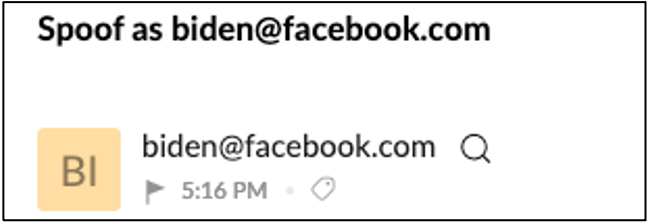
\includegraphics[width=\columnwidth]{graphs/ss_zoho_arc.png}}
%   \centering
%   \caption{An email spoofing \dns{biden@facebook.com} via Fastmail.}
%   \label{fig:ss_zoho_arc}
%   \end{figure}

%Figure~\ref{fig:ss_zoho_arc} in the Appendix illustrates that this attack succeeds without any security warnings, even though the spoofed domain in our
%experiment, \dns{facebook.com}, has a DMARC policy of \textsc{Reject}.



% \subsubsection*{Impact and Mitigation}
% Among providers that we studied, this attack affects customers with
% Zoho email addresses or using Zoho email services,\footnote{We
%   speculate that the above attack also works for customers using Zoho
%   email services, but we are not able to verify this because we are
%   not a Zoho customer.} which together compromise more than 10 million
% potential victims~\cite{Celebrat69:online}.

% However, the attack depends on the existence of providers that allow
% open forwarding and that the receiving provider misinterprets ARC
% headers.  Eliminating either of these factors would foreclose the attack.


\subsection{Abusing Mailing Lists}
\label{subsec:attack_none_mailing_list}

% \subsubsection*{Attack Overview}
The final attack allows an adversary to abuse the forwarding process
used by mailing lists so that spoofed email, which would otherwise
fail DMARC authentication checks, successfully passes both SPF and
DMARC validation.
This attack targets domains with a weak DMARC policy of \textsc{None},
and exploits the way in which many mailing lists rewrite email headers during their forwarding process.
Concretely, this attack allows an adversary to abuse REM header rewriting (\S~\ref{sec:measure_forwarding_mechs_and_arc}) to launder spoofed email through mailing lists such that the forwarded email appears as if it originated from the legitimate sender, even though the original email fails DMARC authentication.\footnote{One such attack used to distribute phishing messages at our institution was part of the impetus for this study.}

% successfully spoof email from any address within an
% organization that uses a vulnerable mailing list service;
% the header rewriting performed by mailing lists makes the spoofed email appear as if originated from the legitimate sender.
% As a result, the attack takes advantage of the header rewriting
% performed by mailing lists to have the spoofed email's headers appear
% as if it originated from the legitimate sender.
%% \geoff{does Sec 4
%%   discuss why mailing lists are designed to work this way, e.g., why
%%   it might have been reasonable for them to work this way?}\alex{Will
%%   add the movitation behind how mailing list operates in sec 2/3,
%%   revisit this later.}

% \subsubsection*{Impact}
%\paragraph{Impact}
\paragraph{Scope}
Our experiments show that attackers can
conduct this attack across all four popular mailing list services: Google
Groups, Mailman, Listserv, and Gaggle.

This attack only affects organizations that use a mailing list configured under their own domain name, and with a DMARC policy of \textsc{None} for their (sub)domain.
While these requirements appear restrictive, prior
work has found that many organizations
(such as major U.S.\ universities) have exactly this configuration~\cite{hutowardsunderstanding}.
Indeed, in querying \dns{.edu} and
\dns{.gov} domains, roughly 10\% of all \dns{.edu}
domains and 5\% of all \dns{.gov} domains are potentially susceptible to this attack.\footnote{As examples, Yale University operates \dnsfn{yale.edu} with a DMARC policy of \textsc{None} and hosts multiple mailing lists using Mailman, and the State of Washington operates a range of mailing lists using Listserv and whose \dnsfn{wa.gov} domain also has a DMARC policy of \textsc{None}.}

Additionally, for mailing lists like Gaggle that do not enforce DMARC
checks before forwarding (Appendix~\ref{subsec:no_dmarc}), this attack affects every organization using their services,
even when the domain has adopted stronger DMARC policies.

% We contribute to the security analysis of mailing lists by
% identifying three possible attacks against all four mailing lists.
% In all three attacks, a spoofed email would be properly forwarded by a mailing list and pass DMARC checks after being forwarded, which makes it very trustworthy. The attacks in this section exploit forwarding mechanisms used by mailing lists and the known weak DMARC policy none.
%
% \alex{HELP NEEDED: I don't how to summarize the three attacks in
% one sentence. See the details below}



% \subsubsection*{Threat Model and Attack Procedure}
%\paragraph{Attack Procedure}
\paragraph{Example}
%In this attack, adversaries control a malicious server that can send spoofed email messages and aim to spoof email from a domain that hosts a mailing list with REM forwarding (Section~\ref{sec:background:fwdingflow}),
%such as Google Groups, Mailman, and Listserv.
%For this attack to work, the spoofed domain must have a DMARC policy of None,
%and the sending email address the attacker wishes to impersonate must have permission to send to the mailing list.
% This attack assumes that only the sender is malicious --- that the adversary controls a server capable of sending spoofed email messages. Additionally, we assume that the domain the adversary wishes to spoof (\dns{univ.edu}) hosts a mailing list with one of these providers,
% such as \dns{list@univ.edu} if they use Google Groups, or \dns{list@listserv.univ.edu} if they use Listserv.
% For this attack to work, \dns{univ.edu} must have a DMARC policy of none,
% and the \dns{univ.edu} email address the attacker wishes to impersonate must have permission to send to the mailing list.
Figure~\ref{fig:google_groups_mech} describes an example of this attack
using Google Groups.
First, an attacker selects a target email address (\dns{someone@univ.edu}) to impersonate in their spoofed email,
and sends the spoofed message from their malicious server to the organization's mailing list (\dns{list@univ.edu}).
Although the email fails DMARC validation,
the mailing list will still accept the message (because \dns{univ.edu}
has a DMARC policy of \textsc{None}).
As part of REM forwarding, the mailing list will rewrite the
\textsc{MAIL FROM} header such that its domain matches the mailing
list's domain, and then forward the email to the list's members.
%(\eg, a new \textsc{MAILFROM} address of
%\dns{xyz@univ.edu}).\footnote{The exact username (the ``xyz'' part) in
%  the \textsc{MAILFROM} address after rewriting depends on the
%  specific implementation.}
As a result, when a recipient's server receives the message it will
successfully pass SPF validation since the domain of the rewritten
\textsc{MAIL FROM} (\dns{univ.edu}) allows the mailing list to send on
its behalf.
Moreover, the spoofed message will also pass DMARC alignment checks,
since the rewriting performed during REM forwarding
ensures that the \textsc{MAIL FROM} and \textsc{FROM} domains are
identical.\footnote{Note that while our examples show this attack
using the organization's top-level domain, it is also effective for
any of the organization's subdomains (if the subdomains also have
DMARC policy \textsc{None}) due to DMARC's inherent relaxed alignment policy.}

During our experiments, we also observed that some mailing list
services, such as Gaggle, do not enforce DMARC policies at all
(Appendix~\ref{subsec:no_dmarc}).
This lack of enforcement allows the attack to succeed regardless of the spoofed domain's DMARC policy.
We provide more details in Appendix~\ref{sec:append_mailing_list_details}.





\section{Ethics and Disclosure}
\label{sec:disclosure}
When sending spoofed email messages in our experiments,
I took deliberate steps to avoid impacting any real users.
First, I only sent spoofed email messages to accounts that I created ourselves.
Second, I initially tested each attack by spoofing domains that I created and controlled for this research.
Once I established that our attacks could succeed using these test domains,
I ran a small set of experiments that spoofed email from real domains (to validate the absence of any unforeseen protection);
however, these email messages were only sent to our test accounts and did not spoof existing, legitimate email addresses from these domains.
Finally, all of our email messages contained innocuous text (e.g., ``a spoofed email'') that would not themselves cause harm.
% even if a message had somehow been misdelivered,
% all of our messages contained innocuous content and thus was unlikely
% to cause harm.

I have disclosed all of the vulnerabilities and attacks to the
affected providers. As of the time of publication, I have received
affirmative feedback from all affected providers and I summarize our
current understanding of their present state here. Zoho has not only
patched the issue with their ARC implementation (also confirmed by
Wang et al.~\cite{wang2022revisiting}, who conducted their
measurements after the patch) and awarded us a bug bounty, but is also
further augmenting the security of its ARC implementation. Microsoft
confirmed the vulnerabilities (with severity ``Important'', the
highest severity assigned to email spoofing bugs) and awarded us a bug
bounty. They have partially fixed the issues by rejecting spoofed email
messages purporting to be from domains that have a DMARC policy of
\textsc{Reject}~\cite{hotmailreject}.
Gaggle confirmed the issues I flagged and stated that they would
start enforcing DMARC. Gmail fixed the issues I reported.  iCloud
partially fixed the issues I reported by not forwarding email
messages that fail DMARC authentication (except for domains with DMARC
policy \textsc{None}). Hushmail fixed the issues I reported by not
forwarding email messages that fail DMARC authentication. Freemail
fixed the issues I reported by not forwarding spoofed email messages
from domains that are their customers. Mail2World attempted to fix the
issues by using spam filters and remains vulnerable. Runbox did not
view the issues I reported as vulnerabilities. Instead, they consider
monitoring account activities post-complaints sufficient.
% I will report on the full set of disclosure feedback and outcomes in the final version of this paper.

\section{Discussion and Mitigation}
We end by summarizing the root causes of the issues I discovered, and discuss potential mitigation strategies.

\subsection{Discussion}
In this work, I examine the complexities introduced by email forwarding to email security. We identify a diverse set of email forwarding mechanisms, assumptions, and features, and demonstrate how they can be combined together to perform evasion attacks. These attacks highlight four fundamental issues.

First, as already demonstrated in prior work and further highlighted in this chapter, email security involves distributed, optional, and independently-configured components implemented by different parties. In such an architecture, the
``authenticity'' of an email is commonly determined by the party with the weakest security settings. While traditionally email is sent directly from sender to receiver, forwarding involves three parties instead of two and introduces an extra layer of complexity. As I have shown, a vulnerable forwarder can jeopardize the security of downstream recipients that do not have problematic configurations or implementations. This inversion of
incentives and capabilities naturally complicates
mitigating forwarding vulnerabilities.

A second problem is that email forwarding has never been fully standardized, despite the longevity and popularity of its use. A lack of standardization has led to ad-hoc implementation decisions, each making different assumptions.
% Indeed, through our large-scale measurements, I identify a diverse set of email forwarding mechanisms, assumptions and features.
This ad-hoc nature of implementations makes it challenging to perform both manual security analysis (analyzing individual implementation decisions is a non-trivial task even for experts) and automated testing (any such tool needs to account for the specific implementations of each provider).
% reasoning about them challenging
% This is in addition to the challenge that there exists no universal dataset of all implementation choices.
% While our large-scale empirical measurements have
% addressed parts of this issue, 
While our large-scale empirical measurements have been able to reveal
the assumptions made by providers and their implications, it has
required substantial manual work.  This manual process is a reflection
of the fact that there exists no unified framework or standard for
implementing email forwarding.
% Any tool that seeks to automate the process needs to adapt to the specific implementations of each provider. In addition, it needs to handle a variety of other issues that are orthogonal to forwarding, such as automatic account creation, authentication, and bypassing anti-bot defenses. All these issues are research topics by themselves.


A third issue is that email is a large, slowly-evolving ecosystem with a wide range of legacy systems and protocols that need to be accommodated.
One example I highlight is the ``outdated'' assumption made by SPF (\S~\ref{subsubsec:spf_incorporation}). When SPF was first designed in the early 2000s, it was common practice for each domain owner to maintain their own mail infrastructure. However, this assumption is obsolete in the modern era, as many domains outsource their email services to third-party providers such as Outlook and Google~\cite{liu2021s}. These large providers often share the same email infrastructure across all customers (both business and personal accounts), violating the assumptions made by SPF. 
To mitigate the risks this reality poses to SPF, providers 
usually prevent users from setting arbitrary values in their FROM header. However, past literature has shown that this defense is not always implemented correctly~\cite{chen2020composition}. We build on top of this prior work by identifying a new attack that can circumvent existing defenses through forwarding (\S~\ref{subsec:attack_open_forwarding}).

Last but not least, the intrinsic nature of email forwarding is to transparently send an existing message to a new address ``on behalf'' of its original recipient --- a goal very much at odds with the anti-spoofing function of protocols such as SPF and DMARC. As such, a range of ad-hoc decisions have been made to increase the deliverability of forwarded email messages, such as using the REM+MOD forwarding mechanism (\S~\ref{sec:measure_forwarding_mechs_and_arc}), treating forwarded messages specially (\S~\ref{subsubsec:relaxed_validation}), and adding DKIM signatures to forwarded messages (\S~\ref{subsubsec:unsolicited_dkim}). As I have demonstrated, 
these decisions can fail to foresee unexpected interactions that lead to vulnerabilities, even with a lot of deliberation.

\subsection{Mitigation}
The attacks I demonstrate highlight the complicated interactions
between email forwarding and existing anti-spoofing mechanisms. We start by reviewing short-term mitigations that could reduce some of the most significant risks I have uncovered. We then discuss challenges in developing more comprehensive solutions, which would require significant changes in either
protocol or operational practices.

A core issue I highlight in this chapter is the ability to forward spoofed email messages to arbitrary recipients, a critical element in each
of the first three attacks in Section~\ref{sec:attacks}. To mitigate this issue, providers could either block spoofed email messages from being forwarded, or enforce that a forwarder can only forward to accounts under their control by requiring explicit confirmation (similar to
the online domain validation used by modern certificate authorities). However, I note that either approach comes with a usability tradeoff, and different providers make choices based on their considerations. Indeed, providers like Gmail and Mail.ru opted for the former option, while others like iCloud and Hushmail opted for the latter.



% allows users to forward spoofed email messages to arbitrary recipients, while Outlook blocks such forwarding~\cite{hotmailreject}.  We also note that while blocking spoofed email messages from being forwarded would protect downstream recipients, it would also break benign forwarding.  For example, a user forwarding a message from a friend to a colleague would be blocked by such a defense. 


% First, I recommend that all mail service providers disable \emph{open
%   forwarding}, and instead require explicit confirmation that the
% forwarding recipient is under the control of the forwarder (similar to
% the online domain validation used by modern certificate authorities). 
% This requirement would prevent the laundering that is a critical element in each
% of the first three attacks in Section~\ref{sec:attacks}.

% Next, a core assumption made by downstream providers is that upstream providers do not forward spoofed email messages. Blocking spoofed email messages from being forwarded is .

As well, I advocate that providers
should enforce a domain's DMARC \textsc{Reject} policy when specified, rather
than substituting a weaker policy.  If Outlook rejected spoofed
email messages from such domains, the impact of the first attack
exploiting SPF incorporation
would
narrow substantially. We understand that Outlook has plans to take such action in the future~\cite{hotmailreject}.


Unfortunately, all the defenses described above reflect a
case of misaligned
%harms
incentives: the recipients of spoofed email (\eg, spam and phishing)
cannot implement this change, but instead need to rely on the entire
ecosystem of providers and forwarding services to adopt such defenses. 

Email providers can also mitigate the second attack (\S~\ref{subsec:attack_relaxed_forwarding_validation}) by eliminating
relaxed validation policies.  This approach would protect their users
from receiving spoofed email without relying on changes by other
platforms or services.  However, to prevent benign forwarding from
breaking will likely require providers to then implement ARC
validation (which in turn places ARC implementation requirements on
external forwarders).

 % Finally, while relaxed validation certainly helps increase the
%deliverability of forwarded email messages, I recommend implementing
%ARC and stick with DMARC policy when possible.

For the final attack (\S~\ref{subsec:attack_none_mailing_list}) that exploits mailing lists, potential mitigations trade usability for security.
% As for the attack on mailing lists, there exists two types of defense mechanisms that trade usability for security.
First, list owners can turn on message moderation and set their mailing lists to be private.
While these measures increase the difficulty of performing email spoofing attacks, they do not rule out the attack entirely. A dedicated attacker might
nonetheless identify a member of the mailing list and craft an email
that fools a list's moderator.
Second, some mailing list services, such as Listserv, support confirm-before-send~\cite{OnmyLIST7:online}, which requests confirmation from the (true) sender address before delivery.  While this mechanism would impose significant overheads in general, these costs might be acceptable by limiting this confirmation requirement to incoming email that fails DMARC authentication checks.

In addition to the short-term mitigations mentioned above that are
specific to forwarding, others~\cite{chen2020composition,shen2020weak}
have proposed solutions such as improving UI notification, building
better testing tools, and revising RFC standards, which are also
important to consider. Additionally, the newly proposed ARC protocol
may also help mitigate some of the issues I have uncovered. However,
ARC is still in the early stages of development and deployment, 
its details are yet to be fleshed out and its effectiveness in
practice remains to be seen.
% \alex{and it may introduce other unexpected issues.} \grant{I think this last bit is a little speculative and there are enough caveats without it.}

Lastly, I note that comprehensively fixing email forwarding would
require a more fundamental set of changes (e.g., redesigning the
entire suite of email security protocols), which will face significant
deployment challenges given the current state of the email ecosystem.
Chief among these challenges is that any new solution designed to fix
forwarding must address backwards compatibility, a task complicated by
email's forty-year-old ecosystem of varied protocols, implementations
and use cases.  Specifically, one must carefully consider how any new
approach interacts and interoperates with existing systems (e.g., mail
providers and filtering service providers) and protocols (e.g., SPF,
DKIM and DMARC).  While security might be enhanced by embracing a
single standard approach to forwarding (e.g., when a message
should be forwarded, what forwarding mechanisms should be used, what
information should be added to forwarded messages, and how the
receiving account should be verified), any such choice will inevitably
  align well with certain providers and conflict with those whose
  existing services have made different choices or who operate under
  different threat models.  Finally, it is not enough to merely
  standardize new protocols, but one must then also incentivize and
  coordinate their universal deployment and operation.  Thus, while
  such an aspirational goal is worthy of attention, it seems likely
  that email will continue to benefit from incremental and reactive
  improvements, such as those discussed earlier, for some time yet.

\section{Conclusion}
\label{sec:discussion}
Internet-based email has been in use since the early 1970s
and the SMTP protocol has been in use since 1980.  It is arguably the
longest-lived text-based communication system in wide use.
Unsurprisingly, its design did not anticipate the range of challenges
we face today and, because of its central role, we have been forced
to upgrade email protocols slowly and with deference to a wide range
of legacy systems and expectations. Perhaps nowhere is this more clear
than around the issue of authentication.  Email protocols have no
widely-used mechanism for establishing the authenticity of sender
addresses, and thus we have focused on authenticating the domain
portion of the email address (largely motivated by spam and phishing).

In this work, using large-scale empirical measurements of 20 prominent email forwarding services, we identify a diverse set of email forwarding mechanisms, assumptions, and features, and demonstrate how they can be combined together to perform four types of evasion attacks. While we are the first academic work to document these attacks, retrospectively examining Mailop~\cite{Mailop96:online}, a prominent mailing list for mail operators, we have also found traces~\cite{RealTraces} of real-world attacks that are similar to what we reported in this chapter. 

The attacks we document exploit four kinds of problems. One fundamental issue is that email security protocols are
distributed, optional, and independently-configured components. This creates a large and complex attack surface with many
possible interactions that cannot be easily anticipated or
administered by any single party. A second problem is that email forwarding was never standardized, leading to ad-hoc implementation decisions that might be vulnerable. A third problem is that protocol assumptions for SPF are grounded at a
point in time and have not been updated as practices have changed. Domains now out-source their mail service to large providers that share mail infrastructure across customers, undermining assumptions made in the design of SPF. Lastly, the intrinsic nature of email forwarding is to transparently send an existing message to a new address ``on behalf'' of its original recipient. 
This creates complex chain-of-trust issues that are at odds with implicit assumptions that mail is sent directly from sender to receiver. Indeed, it is this complication that has driven the creation of ARC.


While there are certain short-term mitigations (\eg, eliminating the use of
open forwarding) that will significantly reduce the exposure to the
attacks we have described here, ultimately email requires a more
solid security footing if it is to effectively resist spoofing
attacks going forwards.


Chapter~\ref{chap:eurosp23}, in part, is a reprint of the material as it appears in Proceedings of the IEEE European Symposium on Security and Privacy 2023. Enze Liu, Gautam Akiwate, Mattijs Jonker, Ariana Mirian, Grant Ho, Geoffrey M. Voelker, and Stefan Savage. The dissertation author was the primary investigator and author of this paper.


%first shed light on the security issues of component-based defense. We
%further examine this issue in the context of email forwarding. For
%example, as we mentioned in Section~\ref{subsec:sender_vulnerability},
%certain providers accept spoofed email messages from domains with
%DMARC none. They rely upon other components (\eg, UI indicators) to
%warn users. As shown by prior work, such components may not exist,
%especially if users are using third-party providers. In this work, we
%further demonstrate such issues in the co


%\alex{can merge with conclusion}
%The attacks we identified have shared some of the high-level concepts. We outline three sources of issues that manifest in the overall picture.
%\alex{Some of the key issues: protocol design vs protocol use; post-hoc protocols not work well for existing use (forwarding); chain of trust; component-based defense; Lack of Standard for forwarding; }

%\paragraph{Inconsistencies between the design and the use of a protocol}
%Protocols designed in the past might make assumptions that do not hold nowadays. Some of the security protocols (\eg, SPF) were designed in the early 2000. SPF was designed with the assumption that each domain will maintain its own mail infrastructure. However, such assumption does not hold in the presence of third-party mail providers these days. To make sure third-party providers can properly send on behalf them, they often have to include their providers' SPF records in their own SPF, potentially allowing others who are sharing the same infrastructure to send on behalf on them. This shared infrastructure is not what SPF was envisioning when designed. As we demonstrated in this work, the discrepancy between the protocol design and its use in practice potential allows an adversary to exploit it.

%Another issue is that post-hoc protocols such as SPF and DMARC do not work well with some of the existing uses. These protocols by design is not compatible with some of the existing uses, which includes email forwarding. The whole email ecosystem has deal with it by making certain assumptions, with potentially relaxed security practices. We demonstrate that this is indeed the case, where providers may exercise a relaxed security policy against forwarded email messages.

%\paragraph{Lack of Standard}
%Unlike security protocols that are well documented and standardized, how email forwarding should be carried out in practice is never standardized. Indeed, as we show this work, there exists at least four broad types of forwarding mechanisms used in the wild. Some of which are well-documented and understood; others are not. Each making different assumption and causes different issues. The whole email ecosystem has to accommodate all of the them, making it hard for the recipient to defend against potential attacks.

%\paragraph{Chain of Trust}
%The email world has also grown complicated enough, that many times email messages are not sent directly from one point to another, but has to go through multiple hops. This inherently makes the defense hard for the recipient. The authenticity of an mail is commonly determined by the party with the weakest security settings in the email forwarding chain. Thus, it is not safe to assume that every party involved has good security practices. Even worse, an adversary can introduce intentionally introduce a forwarder that has bad security practices. As we show in Appendix~\ref{sec:appendix_zoho_attack_details}, even though Gmail does not allow open forwarding, an adversary can still achieve open forwarding by forwarding from Gmail to Outlook, which gives them open forwarding.

%\paragraph{Component-based Defense}
%Chen et al.~\cite{chen2020composition} first shed light on the security issues of component-based defense. We further examine this issue in the context of email forwarding. For example, as we mentioned in Section~\ref{subsec:sender_vulnerability}, certain providers accept spoofed email messages from domains with DMARC none. They rely upon other components (\eg, UI indicators) to warn users. As shown by prior work, such components may not exist, especially if users are using third-party providers. In this work, we further demonstrate such issues in the context of email forwarding, a use case that is less well-considered. We show that even for native MUAs, the one that tend to have better security practices, a dedicated attack can still find holes in the UI system and perform attacks that bypass the defense.




\chapter{No Privacy Among Spies: Assessing the Functionality and Insecurity of Consumer Android Spyware Apps}
\label{chap:pets23}
%-------------------------------------------------------------------------------
\section{Introduction}
%-------------------------------------------------------------------------------

Consumer mobile spyware --- software that covertly gathers information
on a mobile device and transfers that information to a remote server
--- has existed for at least two decades, but has grown significantly
in popularity in recent years.  In one recent study from Norton Labs
~\cite{AYearAft87:online}, the number of devices identified with
spyware apps increased by 63\% between September 2020 and May 2021. A
similar report from Avast saw a 93\% increase in the use of spyware
apps in the UK over a similar period~\cite{UseofSta91:online}.

Sold under a wide variety of brand names --- TheTruthSpy, mSpy,
Flexispy and so on --- these apps are marketed directly to the general
public.  They are relatively cheap (typically between \$30 and \$100
per month), easy to install and do not require specialized technical
know-how to deploy or operate.  Indeed, the only requirements for such
software is \emph{temporary} physical access to the target device
and the ability to install an off-store app.\footnote{Because their features
  violate store policy, app stores like Google Play do not permit the sale of popular spyware apps.}  After
installation, the owner of the target device may have no knowledge
that anything has changed.  But the intimate details of their life can
now be sent to another party, including the contents of their text
messages, email messages, photos taken and received, and even live
recording from their microphone and camera.  Unsurprisingly, such
``stalkerware'' has been implicated in a range of abuses including
intimate partner violence~\cite{chatterjee2018spyware} and
cyberstalking~\cite{woodlock2017abuse}.

Moreover, privacy failures in the ``back end'' software used to store and
display exfiltrated data means that exposure of the victims' private information is not limited to just the abuser who installs the software, but also to miscreants who exploit the insecure design and/or implementations of these apps.
Indeed, a plethora of reports indicate that a broad range of consumer spyware cloud services have been breached,
exposing hundreds of thousands (if not millions) of users' private data~\cite{HackerSt66:online,Companyt8:online,mSpybrea38:online,mSpyCybe86:online,Cerberus12:online,Stalkerw59:online,HackerSt50:online,Spywaref13:online,RetinaXa98:online,Hackercl62:online}.
% Moreover, the exposure of sensitive information is not necessarily
% limited to the party who installs such software, but can be multiplied
% by privacy failures of the ``back end'' software used to store and
% present access to exfiltrated device data.  Indeed, a plethora of reports indicate that a broad range of consumer spyware cloud services have been breached,
% exposing hundreds of thousands (if not millions) of users' private data~\cite{HackerSt66:online,Companyt8:online,mSpybrea38:online,mSpyCybe86:online,Cerberus12:online,Stalkerw59:online,HackerSt50:online,Spywaref13:online,RetinaXa98:online,Hackercl62:online}.

However, while the existence of such software, and the threat it poses,
is well documented in mass media, the technical methods that these apps use to pervasively mine and exfiltrate private data is not well understood.
How does such software hide on
the target device?  How does it acquire the contents of text messages
or of third-party applications? How do these apps monitor a victim's camera or microphone without notifying the user?  Are there a small number of
common techniques for bypassing protections or does each vendor
innovate independently?  Understanding these issues, as well as the
nature of the cloud services used to store the most sensitive data
captured from target devices, is the motivation for this work.

In particular, our paper describes a broad technical investigation
into 14 leading consumer spyware apps for Android-based smart
phones.
Specifically, we seek to answer two key questions:
\begin{itemize}
    \item How do spyware apps achieve their advertised functionalities? We focus on stealthy features that facilitate nonconsensual tracking.
    \item What are the measures taken by spyware apps to protect the data they collect?
\end{itemize}


\begin{facingcaption}{table}
\label{tab:apps_selected}
\renewcommand\tabularxcolumn[1]{>{\RaggedLeft\arraybackslash}p{#1}}
\parindent=0pt
\setbox0=\vbox{%
\vsize\textwidth
\hsize\textheight
\linewidth\hsize
\columnwidth\hsize
\textwidth\hsize
\textheight\vsize

\caption[List of 14 Spyware Apps We Study]{The 14 spyware apps we study, their website domain and its corresponding Tranco ranking, \\their portal domain and its corresponding Tranco ranking, and their APK's target SDK version and \\package name. Tranco rankings taken on May 5th, 2022. \hspace*{0.05in}\\ $^{*}$iKeyMonitor's full package name is `com.sec.android.internet.im.service.im20190419'.}
    
\begin{tabular}{@{}llrlrll@{\hskip 5pt}l}
  App Name             & \multicolumn{2}{c}{Website Domain \hspace*{0.2in}\hfill\hspace*{0.1in} Ranking}  & \multicolumn{2}{c}{Portal Domain \hspace*{0.25in}\hfill\hspace*{0.1in} Ranking} & Target SDK &Package Name                                    \\
  \midrule
  mSPY                 &mspy.com                 &46k             & mspyonline.com  &220k                          &25               &core.update.framework                           \\
  Mobile-tracker-free  &mobile-tracker-free.com  &54k             &mobile-tracker-free.com  &54k                   &28                      &mobile.monitor.child2021                        \\
  Clevguard            &clevguard.com            &69k             & clevguard.com  &69k                            &28             &com.kids.pro                                    \\
  \ltgrey HoverWatch   &hoverwatch.com           &87k             &hoverwatch.com  &87k                            &28          &com.android.core.mntw                           \\
  \ltgrey Flexispy     &flexispy.com             &107k            &flexispy.com &107k                              &22          &com.fp.backup                                   \\
  \ltgrey Spyic        &spyic.com                &152k            &spyic.com  &152k                                &22         &com.sc.spyic.v3                                 \\
  Spyhuman             &spyhuman.com             &179k            & spyhuman.com  &179k                            &22              &m.mobile.control                                \\
  TheTruthSpy          &thetruthspy.com          &214k            & thetruthspy.com &214k                          &28               &com.systemservice                               \\
  iKeyMonitor          &ikeymonitor.com          &230k            &emcpanel.com  &1.1m                             &23        &com.sec...im20190419$^{*}$  \\
  \ltgrey Cerberus     &cerberusapp.com          &251k            & cerberusapp.com  &251k                         &23             &com.lsdroid.cerberus                            \\
  \ltgrey Spy24        &spy24.app                &284k            & spy24.net  &2.4m                               &29          &net.spy24.wifi                                  \\
  \ltgrey Spapp        &spappmonitoring.com      &421k            &spappmonitoring.com  &421k                      &26                  &com.monspap.alarm                               \\
  Meuspy               &meuspy.com               &485k            & meuspy.com  &485k                              &32        &br.com.sistema.aplicativo                       \\
  Highstermobile       &highstermobile.com       &590k            &evt17.com  &1.5m                                &30       &org.secure.smsgps                               \\
\end{tabular}
\singlespacing
}
\centerline{\rotatebox{90}{\box0}}
\end{facingcaption}



To address these questions empirically, we reverse engineered 14 of
the most popular consumer spyware apps. 
In analyzing their behavior
we make three primary contributions:
\begin{itemize}
  \item We performed the first comprehensive and in-depth analysis of mechanisms used by consumer spyware apps to bypass or trick system level isolation across a range of different feature categories.
  \item In addition to confirming the broad use of some techniques identified in the mobile malware literature (e.g., abusing ``accessibility'' APIs), we identified two novel abuses of Android
    APIs (new techniques of invisible camera access and hiding app icons). We also document that Android's threat model does not include abuses of their APIs that allow apps to conceal their icon.
  \item We tested spyware apps \emph{in
  situ} in a carefully monitored environment and analyzed their communications with the cloud service components.  We believe our work is also the first academic effort to document in detail a range of privacy deficiencies (e.g.,
  data sent in plaintext and cloud services with insecure direct object references (IDOR~\cite{IDOR62:online, IDORCWE:online}) for the contents of phone data).
\end{itemize}

Together, we believe that this work further sharpens the community's understanding
of consumer mobile spyware, providing guidance both for phone OS
vendors and regulators in their efforts to mitigate the use and
availability of such software.





\section{Spyware}

To provide context for our study, I first describe how spyware is
used in general and then describe how I selected the specific spyware
apps I investigate.

\subsection{Spyware Use}

Spyware enables an adversary to surreptitiously record the activities,
behavior, and location of a victim based on the victim's phone usage.
These invasive apps have a wide range of capabilities for
monitoring the victim, and do so using existing Android APIs without
needing root access.

To install these apps, the adversary first creates an account on the spyware's web portal
interface and purchases a subscription, if required.  The adversary then
requires physical access to the victim's device to download and
install the spyware app.  When installing, the app requests an
extensive set of Android permissions as the basis for performing its
monitoring activity.  The adversary readily grants these permissions to
the app, a step which entirely undermines the Android app permission
model.  The adversary then signs in to the app on the device, typically
using the same credentials used by the web portal, and links the
victim's device with the adversary's account on the spyware portal.

Subsequently, the adversary no longer needs physical access to the victim's device, and
can remotely control the actions of the app via the online spyware portal.
The spyware app both passively collects data on the victim's device (e.g.,
location, text messages, calls, etc.), and also allows the adversary to
perform on-demand remote actions like covertly recording audio and
video, taking app screenshots, etc.

Although spyware authors exhibit tremendous effort and creativity in subverting
Android sandbox protections to implement their capabilities, many apps spend
much less effort in protecting the data that they exfiltrate and store on
their backend servers. Later, in Section~\ref{sec:data-leak} I
describe several vulnerabilities in spyware apps that put the victim's
data at risk to a third-party attacker.



\subsection{Spyware App Selection}
\label{subsec:app_selection}

%% Our work focuses on off-store spyware apps since they request
%% a significant number of permissions (from 15 to 53, median 44), implement many
%% privacy-invasive capabilities (Section~\ref{sec:api-abuse}), and do not require root to function. In comparison,
%% apps that are available on the Google Play Store (typically these are apps
%% intended for consensual subordinate tracking of a child or employee) are less
%% likely to request dangerous permissions such as access to the camera, and
%% other permissions highly susceptible to abuse like
%% accessibility~\cite{feal2020angel}.


For our analysis, I chose 14 distinct leading consumer Android spyware
apps.\footnote{Often the same spyware app is available under multiple
  names. I identify and avoid choosing duplicate apps.}  I focus on
Android-based spyware because most of the mobile spyware market
appears to be focused there. Since curated app stores like Google Play do not permit
the sale of such apps, in practice they must be side-loaded off-store, a process
that Apple does not support.  As a result, consumer mobile spyware only operates on ``rooted'' iPhones.  Rooting an iPhone can be a
technically involved operation (one popular guide to jailbreaking the
iPhone involves 41 distinct steps \cite{howToJailbreakIphone:online}) and one that can take significant
time to complete --- both requirements at odds with the broad,
non-technical customer base such apps are marketed to. I also focus on leading spyware apps as they are the apps that more people are exposed to and they are more likely to be innovative (new features could potentially bring them more customers).

In our selection process, I started with the 18 off-store spyware apps identified by Chatterjee et al.~\cite{chatterjee2018spyware}. I augmented our set of apps by taking the intersection of two major industry reports (\cite{esetandr4:online} and~\cite{Tekstalk86:online}) that listed spyware apps.\footnote{We take the intersection of both reports because (a) the definition of consumer spyware is vague; and (b) the collection process is ad-hoc and differs for each report. Apps in the intersection represent consensus among these disparate classifications.} Next, I sorted all the apps based on the Tranco ranking~\cite{pochat2018tranco} of their website domain (snapshot taken on May 5th, 2022).  I filtered out apps that were distributed via Google Play (since, to appear in
the store, they do not have compelling spyware capabilities)
%% apps distributed via Google Play have very limited capabilities
or broken (e.g., not reachable or no longer accepting payments).
%% \alex{One way to avoid mentioning off-store is exlaining why I ignored apps distributed via google store (which is my current version); another option is to squeez in the off-store part somewhere in the intro; }
For apps that are rebranded versions of other apps, I consider them duplicates and did not examine them separately.

From the top 25 most popular apps, I identified 14 distinct apps which I used in our study. The apps in this set are produced by a wide spectrum of vendors, with a broad array of capabilities, and cover the majority of apps identified in prior work~\cite{chatterjee2018spyware} (10 out of the 14 apps that are still alive). Moreover, I find significant overlap in the low-level technical implementation of spyware capabilities:  all but three techniques described in Section~\ref{sec:api-abuse} are discovered after reverse engineering the top five most popular apps (in terms of website domain ranking), and no new techniques are found after the 11th ranked app (Spy24).\footnote{While I do continue to find different variants or implementation of the same technique, I view these as minor details.}
% \alex{added a few words that talks about these apps being sorted}
The lack of new techniques discovered among less popular apps in our set suggests that the apps I study capture a representative set of techniques used in practice.


Table~\ref{tab:apps_selected} shows the list of spyware apps I chose, their website domain and its corresponding Tranco ranking, their web portal domain and its corresponding Tranco ranking, and their APK's target SDK version and package name.


\section{Spyware Abuse of Android APIs}
\label{sec:api-abuse}

In this section, I explain how spyware apps implement various privacy invasive
capabilities using existing APIs supported by the Android OS.
%These different capabilities enable attackers to achieve various goals: monitor a user's online activities (e.g., the messages they send, the photos they take, etc.), abuse the device to spy on the user's activity in the physical world (e.g., using the victim's phone to silently record audio and video or track their location), stealthily spy on their victim without their knowledge or consent, and persistently conduct their spying over a long period of time.
I start by discussing our methodology for identifying these capabilities and uncovering their associated implementations.
I then summarize the set of basic capabilities (\S~\ref{subsec:features_enabled_by_permission}) that either do not require any permissions or are enabled just by acquiring permissions,
and group
all of the other capabilities that I study into three categories based on their goals: stealthily
collecting a victim's information (\S~\ref{subsec:data_gathering}), hiding the app's presence on the phone (\S~\ref{subsec:hiding_the_app}), and persistently
spying over a long period of time (\S~\ref{subsec:persistence}).
For each category, we
describe
each capability in the category and its associated implementations, and end
the category by discussing potential mitigations.
%We conclude this section with a short discussion.

%\grant{Suggestion for an extra overview sentence: These different features
%enable attackers to achieve four invasive goals: monitor a user's online
%activities (e.g., the messages they send, the photos they take, etc.), abuse the
%device to spy on the user's activity in the physical world (e.g., using the
%victim's phone to silently record audio and video or track their location),
%stealthily spy on their victim without their knowledge or consent, and
%persistently conduct their spying over a long period of time.} \grant{My
%suggested wording above is a bit clunky, but I think it would be helpful to
%structure these features in terms of slightly high-level goals that stalkers
%want to achieve (capturing different kinds of the victim's digital + physical
%activity, stealthily performing their spying, and being able to spy on the
%victim for long periods of time) and present an overview of this framing
%upfront.}

%We start by describing how I select the features and our methodology for
%uncovering implementations associated with each feature
%(Section~\ref{subsec:misuse_discovery}). Next, I present X features and their
%implementations, and discuss potential mitigation solutions
%(Section~\ref{subsec:api_abuse_results}).

% \begin{figure*}[h]
% \includegraphics[width=\textwidth]{fig/APIAbuse.pdf}
% \caption{Summary of features studied}
% \label{tab:feature_summary}
% \end{figure*}


% \todo{rotate the table}
% \begin{table*}[t]
%   \centering
%     \begin{tabular}{p{3.0cm}p{4.7cm}llllllllllllll}
%        Category                                                &Capabilities                          &\rotatebox{90}{mSPY}  &\rotatebox{90}{Mobile-tracker-free}  &\rotatebox{90}{Clevguard}  &\rotatebox{90}{HoverWatch}  &\rotatebox{90}{Flexispy}  &\rotatebox{90}{Spyic}  &\rotatebox{90}{Spyhuman}  &\rotatebox{90}{TheTruthSpy}  &\rotatebox{90}{iKeyMonitor}  &\rotatebox{90}{Cerberus}  &\rotatebox{90}{Spy24}  &\rotatebox{90}{Spapp}  &\rotatebox{90}{Meuspy}  &\rotatebox{90}{Highstermobile}  \\
%       \midrule
%     \multirow{11}{*}{\shortstack[l]{Basic Capabilities (\S~\ref{subsec:features_enabled_by_permission})}}   &Ambient Recording                     &                      &\checkmark                           &                 &                            &\checkmark                &                       &\checkmark                &\checkmark                   &\checkmark                   &\checkmark                &\checkmark             &\checkmark             &\checkmark              &                                \\
%                                                                                                      &Calendar                              &\checkmark            &\checkmark                           &\checkmark                 &\checkmark                  &\checkmark                &\checkmark             &\checkmark                &\checkmark                   &\checkmark                   &\checkmark                &\checkmark             &\checkmark             &\checkmark              &\checkmark                      \\
%                                                                                                      &Call Logs                             &\checkmark            &\checkmark                           &\checkmark                 &\checkmark                  &\checkmark                &\checkmark             &\checkmark                &\checkmark                   &\checkmark                   &\checkmark                &\checkmark             &\checkmark             &\checkmark              &\checkmark                      \\
%                                                                                                      &Clipboard                             &                      &\checkmark                           &                           &                            &                          &                       &                          &\checkmark                   &\checkmark                   &                          &\checkmark             &                       &                        &                                \\
%                                                                                                      &Contacts                              &\checkmark            &\checkmark                           &\checkmark                 &\checkmark                  &\checkmark                &\checkmark             &\checkmark                &\checkmark                   &\checkmark                   &\checkmark                &\checkmark             &\checkmark             &\checkmark              &\checkmark                      \\
%                                                                                                      &Info of Other Applications            &\checkmark            &\checkmark                           &\checkmark                 &\checkmark                  &\checkmark                &\checkmark             &\checkmark                &\checkmark                   &\checkmark                   &\checkmark                &\checkmark             &\checkmark             &\checkmark              &\checkmark                      \\
%                                                                                                      &Location                              &\checkmark            &\checkmark                           &\checkmark                 &\checkmark                  &\checkmark                &\checkmark             &\checkmark                &\checkmark                   &\checkmark                   &\checkmark                &\checkmark             &\checkmark             &\checkmark              &\checkmark                      \\
%                                                                                                      &Network Info                          &\checkmark            &\checkmark                           &\checkmark                 &\checkmark                  &\checkmark                &\checkmark             &\checkmark                &\checkmark                   &\checkmark                   &\checkmark                &\checkmark             &\checkmark             &\checkmark              &\checkmark                      \\
%                                                                                                      &Phone Info                            &\checkmark            &\checkmark                           &\checkmark                 &\checkmark                  &\checkmark                &\checkmark             &\checkmark                &\checkmark                   &\checkmark                   &\checkmark                &\checkmark             &\checkmark             &\checkmark              &\checkmark                      \\
%                                                                                                      &SMS or MMS                            &\checkmark            &\checkmark                           &\checkmark                 &\checkmark                  &\checkmark                &\checkmark             &\checkmark                &\checkmark                   &\checkmark                   &\checkmark                &\checkmark             &\checkmark             &\checkmark              &\checkmark                      \\
%                                                                                                      &Shared Media Files                    &\checkmark            &\checkmark                           &\checkmark                 &\checkmark                  &\checkmark                &\checkmark             &\checkmark                &\checkmark                   &\checkmark                   &\checkmark                &\checkmark             &\checkmark             &\checkmark              &\checkmark                      \\
%     \hline
% %    \multirow{4}{*}{\shortstack[l]{\S~3.3}} & \multirow{4}{*}{\shortstack[l]{Data Gathering}}         &Invisible camera access               &                      &\checkmark                           &\checkmark                 &\checkmark                  &\checkmark                &                       &\checkmark                &\checkmark                   &\checkmark                   &\checkmark                &\checkmark             &\checkmark             &\checkmark              &\checkmark                      \\
%     \multirow{4}{*}{\shortstack[l]{Data Gathering (\S~\ref{subsec:data_gathering})}}         &Invisible camera access               &                      &\checkmark                           &\checkmark                 &\checkmark                  &\checkmark                &                       &\checkmark                &\checkmark                   &\checkmark                   &\checkmark                &\checkmark             &\checkmark             &\checkmark              &\checkmark                      \\
%                                                                                                      &Invisible microphone access                  &                      &\checkmark                           &\checkmark                 &\checkmark                  &\checkmark                &                       &\checkmark                &\checkmark                   &\checkmark                   &                          &\checkmark             &\checkmark             &\checkmark              &                                \\
%                                                                                                      &Accessing protected data               &\checkmark            &\checkmark                           &\checkmark                 &\checkmark                  &\checkmark                &\checkmark             &\checkmark                &\checkmark                   &\checkmark                   &\checkmark                &\checkmark             &\checkmark             &\checkmark              &\checkmark                      \\
%                                                                                                      &Taking screenshots                    &\checkmark            &\checkmark                           &\checkmark                 &\checkmark                  &                          &                       &\checkmark                &                             &\checkmark                   &                          &\checkmark             &\checkmark             &\checkmark              &                                \\
%     \hline
% %    \multirow{3}{*}{\shortstack[l]{\S~3.4}} & \multirow{3}{*}{\shortstack[l]{Hiding the App}}  &Hiding app icon                       &\checkmark            &\checkmark                           &\checkmark                 &\checkmark                  &\checkmark                &\checkmark             &\checkmark                &\checkmark                   &\checkmark                   &\checkmark                &\checkmark             &\checkmark             &\checkmark              &                                \\
%     \multirow{3}{*}{\shortstack[l]{Hiding the App (\S~\ref{subsec:hiding_the_app})}}  &Hiding app icon                       &\checkmark            &\checkmark                           &\checkmark                 &\checkmark                  &\checkmark                &\checkmark             &\checkmark                &\checkmark                   &\checkmark                   &\checkmark                &\checkmark             &\checkmark             &\checkmark              &                                \\
%                                                                                                      &Launching a hidden app                &                      &\checkmark                           &                           &\checkmark                  &\checkmark                &\checkmark             &\checkmark                &\checkmark                   &\checkmark                   &\checkmark                &\checkmark             &\checkmark             &\checkmark              &                                \\
%                                                                                                      &Hide from recents screen              &\checkmark            &\checkmark                           &\checkmark                 &\checkmark                  &\checkmark                &\checkmark             &\checkmark                &                             &\checkmark                   &\checkmark                &\checkmark             &                       &\checkmark              &\checkmark                      \\
%     \hline
% %    \multirow{2}{*}{\shortstack[l]{\S~3.5}} & \multirow{2}{*}{\shortstack[l]{Persistence}}            &Obscuring the uninstallation process  &\checkmark            &\checkmark                           &\checkmark                 &                            &\checkmark                &                       &\checkmark                &\checkmark                   &\checkmark                   &\checkmark                &\checkmark             &\checkmark             &\checkmark              &                                \\
%     \multirow{2}{*}{\shortstack[l]{Persistence (\S~\ref{subsec:persistence})}}            &Obscuring the uninstallation process  &\checkmark            &\checkmark                           &\checkmark                 &                            &\checkmark                &                       &\checkmark                &\checkmark                   &\checkmark                   &\checkmark                &\checkmark             &\checkmark             &\checkmark              &                                \\
%                                                                                                      &Creating "diehard" services           &\checkmark            &\checkmark                           &\checkmark                 &\checkmark                  &\checkmark                &\checkmark             &\checkmark                &\checkmark                   &\checkmark                   &\checkmark                &\checkmark             &\checkmark             &\checkmark              &\checkmark                      \\
%     \hline
% %     \end{tabular}
%     \caption{\todo{format}
%       %, otherwise I leave the corresponding cell in the table blank.
%       }
%   \end{table*}



\begin{facingcaption}{table}
\caption[Summary of Spyware Capabilities Studied]{Summary of capabilities studied. A star denotes that an app implements a particular capability.}
\label{tab:feature_summary}
\renewcommand\tabularxcolumn[1]{>{\RaggedLeft\arraybackslash}p{#1}}
\parindent=0pt
\setbox0=\vbox{%
\vsize\textwidth
\hsize\textheight
\linewidth\hsize
\columnwidth\hsize
\textwidth\hsize
\textheight\vsize


\begin{tabular}{p{5.0cm}p{4.7cm}llllllllllllll}
    Category                                                &Capabilities                          &\rotatebox{90}{mSPY}  &\rotatebox{90}{Mobile-tracker-free}  &\rotatebox{90}{Clevguard}  &\rotatebox{90}{HoverWatch}  &\rotatebox{90}{Flexispy}  &\rotatebox{90}{Spyic}  &\rotatebox{90}{Spyhuman}  &\rotatebox{90}{TheTruthSpy}  &\rotatebox{90}{iKeyMonitor}  &\rotatebox{90}{Cerberus}  &\rotatebox{90}{Spy24}  &\rotatebox{90}{Spapp}  &\rotatebox{90}{Meuspy}  &\rotatebox{90}{Highstermobile}  \\
    \midrule
    \multirow{3}{*}{\shortstack[l]{Basic Capabilities (\S~\ref{subsec:features_enabled_by_permission})}}   &Ambient Recording                     &                      &\checkmark                           &                 &                            &\checkmark                &                       &\checkmark                &\checkmark                   &\checkmark                   &\checkmark                &\checkmark             &\checkmark             &\checkmark              &                                \\
                                                                                       &SMS or MMS                            &\checkmark            &\checkmark                           &\checkmark                 &\checkmark                  &\checkmark                &\checkmark             &\checkmark                &\checkmark                   &\checkmark                   &\checkmark                &\checkmark             &\checkmark             &\checkmark              &\checkmark                      \\
                                                                                                     &Shared Media Files                    &\checkmark            &\checkmark                           &\checkmark                 &\checkmark                  &\checkmark                &\checkmark             &\checkmark                &\checkmark                   &\checkmark                   &\checkmark                &\checkmark             &\checkmark             &\checkmark              &\checkmark                      \\
    \hline
%    \multirow{4}{*}{\shortstack[l]{\S~3.3}} & \multirow{4}{*}{\shortstack[l]{Data Gathering}}         &Invisible camera access               &                      &\checkmark                           &\checkmark                 &\checkmark                  &\checkmark                &                       &\checkmark                &\checkmark                   &\checkmark                   &\checkmark                &\checkmark             &\checkmark             &\checkmark              &\checkmark                      \\
    \multirow{4}{*}{\shortstack[l]{Data Gathering (\S~\ref{subsec:data_gathering})}}         &Invisible camera access               &                      &\checkmark                           &\checkmark                 &\checkmark                  &\checkmark                &                       &\checkmark                &\checkmark                   &\checkmark                   &\checkmark                &\checkmark             &\checkmark             &\checkmark              &\checkmark                      \\
                                                                                                     &Invisible microphone access                  &                      &\checkmark                           &\checkmark                 &\checkmark                  &\checkmark                &                       &\checkmark                &\checkmark                   &\checkmark                   &                          &\checkmark             &\checkmark             &\checkmark              &                                \\
                                                                                                     &Accessing protected data               &\checkmark            &\checkmark                           &\checkmark                 &\checkmark                  &\checkmark                &\checkmark             &\checkmark                &\checkmark                   &\checkmark                   &\checkmark                &\checkmark             &\checkmark             &\checkmark              &\checkmark                      \\
                                                                                                     &Taking screenshots                    &\checkmark            &\checkmark                           &\checkmark                 &\checkmark                  &                          &                       &\checkmark                &                             &\checkmark                   &                          &\checkmark             &\checkmark             &\checkmark              &                                \\
    \hline
%    \multirow{3}{*}{\shortstack[l]{\S~3.4}} & \multirow{3}{*}{\shortstack[l]{Hiding the App}}  &Hiding app icon                       &\checkmark            &\checkmark                           &\checkmark                 &\checkmark                  &\checkmark                &\checkmark             &\checkmark                &\checkmark                   &\checkmark                   &\checkmark                &\checkmark             &\checkmark             &\checkmark              &                                \\
    \multirow{3}{*}{\shortstack[l]{Hiding the App (\S~\ref{subsec:hiding_the_app})}}  &Hiding app icon                       &\checkmark            &\checkmark                           &\checkmark                 &\checkmark                  &\checkmark                &\checkmark             &\checkmark                &\checkmark                   &\checkmark                   &\checkmark                &\checkmark             &\checkmark             &\checkmark              &                                \\
                                                                                                     &Launching a hidden app                &                      &\checkmark                           &                           &\checkmark                  &\checkmark                &\checkmark             &\checkmark                &\checkmark                   &\checkmark                   &\checkmark                &\checkmark             &\checkmark             &\checkmark              &                                \\
                                                                                                     &Hide from recents screen              &\checkmark            &\checkmark                           &\checkmark                 &\checkmark                  &\checkmark                &\checkmark             &\checkmark                &                             &\checkmark                   &\checkmark                &\checkmark             &                       &\checkmark              &\checkmark                      \\
    \hline
%    \multirow{2}{*}{\shortstack[l]{\S~3.5}} & \multirow{2}{*}{\shortstack[l]{Persistence}}            &Obscuring the uninstallation process  &\checkmark            &\checkmark                           &\checkmark                 &                            &\checkmark                &                       &\checkmark                &\checkmark                   &\checkmark                   &\checkmark                &\checkmark             &\checkmark             &\checkmark              &                                \\
    \multirow{2}{*}{\shortstack[l]{Persistence (\S~\ref{subsec:persistence})}}            &Obscuring the uninstallation process  &\checkmark            &\checkmark                           &\checkmark                 &                            &\checkmark                &                       &\checkmark                &\checkmark                   &\checkmark                   &\checkmark                &\checkmark             &\checkmark             &\checkmark              &                                \\
                                                                                                     &Creating "diehard" services           &\checkmark            &\checkmark                           &\checkmark                 &\checkmark                  &\checkmark                &\checkmark             &\checkmark                &\checkmark                   &\checkmark                   &\checkmark                &\checkmark             &\checkmark             &\checkmark              &\checkmark                      \\
    \hline
    \end{tabular}

\singlespacing
}
\centerline{\rotatebox{90}{\box0}}
\end{facingcaption}


\subsection{Methodology}
\label{subsec:misuse_discovery}


%% \geoff{I'm now thinking that I can use Section 2 to set the context:
%%   how spyware is used + our app selection process.  we'll then put the
%%   methodologies back into Sections 3 and 4.}

% Breaking into the vault: Privacy, security and forensic analysis of Android vault applications
% Transfiguring of an Android App Using Reverse Engineering
% Reverse engineering of mobile applications
% https://www.uit.edu.mm/storage/2020/09/No.-5.pdf
I gather a list of privacy invasive capabilities from two sources: (1)
capabilities advertised and offered by spyware apps; and (2) prior
academic papers and industry reports described in Section~\ref{sec:related_work} that look at how the Android API
can be used to achieve such unintended functionality.
Table~\ref{tab:feature_summary} summarizes the capabilities I study
and shows which spyware apps implement them.
To understand how the spyware apps implement their nefarious capabilities, I reverse engineered and analyzed each app. Our approach consists of three steps.

\textbf{Preparation.} I acquire the latest APKs of spyware apps by directly downloading them from their websites. I use \texttt{APKTOOL}~\cite{ApktoolA72:online} to disassemble the APKs and obtain the corresponding manifest and smali code.\footnote{Smali is a human-readable represenation of the Dalvik bytecode used by Android apps.} I also decompile the APK to Java source using \texttt{JADX}~\cite{skylotja9:online}.

\textbf{Manual Investigation.}
For each capability, I manually analyzed the app manifest and the decompiled Java code to determine how
each capability was implemented using the standard Android API: I manually located the API primitives associated with each capability, examined the relevant control flow, and confirmed that the primitives I identified were reachable. While I primarily used the decompiled Java code for
analysis, I reviewed the smali code when necessary (e.g., when a function fails
to decompile). Since the variable and method names were often obfuscated, I renamed them to human-readable ones as I examined the decompiled Java code (our naming annotations are available upon request).

Once I discovered an implementation for a particular capability and
the API primitives one app used, I expedited our search process
for other apps by searching for use of the same API primitives, and manually
reviewed the results to remove false positives. If this API similarity
approach did not yield results, I reverted back to manually
inspecting the code.

I use two heuristics to guide our manual investigation process.
First, many apps can receive remote commands (e.g., using third-party
libraries such as Firebase~\cite{Firebase21:online}).  The method
responsible for dispatching remote commands is a useful top-down
starting place for identifying the underlying implementation (e.g.,
following the methods it calls in response to remote commands).  For
apps that do not receive remote commands, they operate as background
services to covertly collect user data. These background services
often are responsible for dispatching various tasks and contain useful
leads. Second, for any capability, there are limited ways to implement
it using Android API primitives, and many of them are publicly
documented (e.g., capturing audio through \texttt{MediaRecorder}). Searching for these API primitives in the code helps to
quickly locate methods associated with a capability. Additionally,
once I identified an implementation of a capability, I examined its
control flow in a bottom-up fashion to identify the operation that
would trigger its execution (typically leading back to dispatch
methods).

\textbf{Confirmation.} For each implementation of a capability (and
related API primitives) I discover, I verified our analysis conclusions
by developing an app using the same API primitives and
testing it on a Pixel 4 phone running Android 11. I also installed and ran each spyware app to ensure the capabilities I observed were indeed enabled.
Since the majority of the apps we
study have been implemented using Android APIs up to Android 11, we
discuss their implementations in that context. However, I also
discuss the impact changes in Android 12 can have on the spyware apps.

%\subsubsection{Code Release}
% \textbf{Code Release.}  Our code that implements all the API
% primitives discovered in this paper is available upon
% request. Similarly, the annotated class and variable names are
% available upon request (which can be used to reproduce our results
% after independently acquiring the corresponding APK files). To avoid
% potential copyright infringement risks, I do not provide the
% decompiled and annotated source code itself.

%% I focus our discussion on Android 11 and earlier, and discuss the
%% impact of Android 12 when relevant. \alex{We need a machine that runs
%%   Android 12? Big enhancements include a persistent indicator and
%%   privacy dashboard}


%\subsection{Abusive and Non-abusive API Usage}
%\alex{maybe this is not necessary}
%We define Android API misuse as: any functionality that relies on using the
%Android platform API in ways that violate either Play Store policies or the
%clearly intended usage of the platform per the Android developer documentation.
%Broadly speaking, I focus on abusing API to: covertly collect private user or
%app data, hide app traces, and survive across reboots and kills.


% \subsection{Results}
% \label{subsec:api_abuse_results}
% I start by briefly discussing a set of features that are enabled after
% acquiring certain permissions. These features are only protected by
% permissions and many are not noticeable by users. Next, I detail how spyware
% apps implement features that allow them to exfiltrate data covertly, stay
% stealthy, and persist on the target device.

\subsection{Basic Capabilities}
\label{subsec:features_enabled_by_permission}
As seen in Table~\ref{tab:feature_summary}, all spyware apps support a large, common set of basic capabilities for collecting sensitive user data.
These capabilities either do not require any permission (e.g., clipboard) or are easily enabled after obtaining particular Android permissions (e.g., reading SMS messages, contacts, call logs, etc.). Spyware apps can obtain these capabilities simply by
requesting the associated permissions in the manifest at installation or their first run.
Additionally, by design most of these capabilities
(except for location and ambient recording) do not provide any notification to
the user and are straightforward to implement.


\subsection{Data Gathering}
\label{subsec:data_gathering}
Spyware apps seek to stealthily collect a victim's information without being noticed. In this section, I describe how they covertly access the camera, the microphone, and protected data of other apps, as well as how they take screenshots all without the victim's knowledge.

\subsubsection*{Capability \#1: Invisible Camera Access}
\label{subsubsec:invisible_cam}
Spyware apps use a device's camera to take pictures, record videos, and stream live
videos. To remain hidden from the victim, spyware apps need to access the camera
without being noticed. The apps I studied use three methods to achieve
surreptitious camera access: (1) using an invisible preview; (2) intercepting raw
frames without a preview; and (3) using an invisible browser.
% \alex{added a novelty statement}
While the first technique is well-documented in the malware literature (e.g., Yan et al.~\cite{yan2019understanding}), the second and third techniques
have not been reported before and reflect
the creativity that spyware authors continue to apply in
abusing the Android API to implement their capabilities.

% (unique to Spy24);

% I start by briefly explaining how camera works. Readers who are interested in
% the details should refer to Android's developer
% guide~\cite{Cameraca74:online}. Android apps can capture images or videos by
% creating a camera capture session. To create a camera session, apps need to
% provide it with one or more output target buffers. One type of target buffer
% is SurfaceView, which can be used as a preview to display the image or video
% directly to the user. Other types of target buffers include ImageReader and
% SurfaceTexture, which are used for more advanced scenarios and not visible to
% users. If spyware apps uses SurfaceView as the target buffer, they need to
% hide the preview being displayed. This can be done by setting the preview size
% to 1x1.

% they can stay unnoticed by creating a SurfaceView that is not visible
% (typically of size 1x1).

\textbf{Invisible Preview}. One way to use the camera is to create a preview that displays an image or video to users. Once a preview is started, apps can take pictures or record videos. Benign apps (such as selfie apps) use a preview so that users can see the current status of the camera. Spyware apps, in contrast, seek to hide this preview by setting the preview to an invisible size (typically a 1x1 pixel) or making the preview transparent.
% \alex{moved the novelty statement up}

\textbf{Raw Frames Without a Preview}.
Spyware apps can also access the output of the camera without displaying a
preview using advanced camera features supported by
Android~\cite{Cameraca74:online}. For example, apps can capture raw frames from
the camera with either an \texttt{ImageReade}r~\cite{Cameraca74:online} or
\texttt{SurfaceTexture}~\cite{SurfaceT78:online}, neither of which requires showing a
preview on the screen.
Benign apps (such as photo apps) use these
features for advanced operations such as frame-by-frame processing. Spyware
apps, on the other hand, use these features to capture raw frames, either saving
the frames locally or streaming the frames to a remote server, all without the
victim noticing. While the expectation for such advanced features is that the
processed frames will be displayed to users eventually (which is normally the
case for benign apps), this by no means is enforced. Finally, I note that four
apps rely on the third-party library WebRTC (or its variants) to achieve this functionality (WebRTC uses both \texttt{ImageReader} and \texttt{SurfaceTexture}).

%\geoff{does webrtc then use an ImageReader or SurfaceTexture?}\alex{fixed}

\textbf{Invisible Browser}. Unique to Spy24, this app uses an invisible
\texttt{WebView}~\cite{WebViewA25:online} (an in-app browser) with a 1x1 pixel size for
streaming live videos. While the browser may be invisible, the app can stream
full camera resolution to a Spy24 server.
%\geoff{Alex confirm?}\alex{correct}
\texttt{WebView} allows users to browse web content in an app while providing advanced
configuration options to developers. Spy24, in this instance, programmatically sets
the user agent, enables JavaScript, and disables the cache. This configuration
flexibility provided by \texttt{WebView} is necessary for streaming via a web browser.
%% as standard web browsers like Chrome have limited configuration
%% flexibility.\geoff{by hard to achieve, you mean hard to achieve
%% invisibly?}\alex{fixed}

Once the browser is configured, it accesses the camera via a JavaScript version
of WebRTC (loaded dynamically) and streams live video back to a Spy24 server.
This approach evades static analysis that examines API calls in the APK file, as
the JavaScript file is loaded during runtime.
Listing~\ref{lst:invisible_browser_code} shows a snippet of code that
demonstrates how Spy24 streams video with an invisible browser. First, it adds the 1x1 \texttt{WebView} as an overlay.  It then sets a specific user
agent to act as a trigger. Upon contacting the server, the \texttt{WebView} loads a
JavaScript file that activates the camera if the \texttt{WebView} has the specified user
agent.

%\vspace{0.5cm}
%\hspace{-0.1\linewidth}
%\begin{minipage}{0.5\textwidth}
\begin{lstlisting}[basicstyle=\small\ttfamily,caption={Code snippet that demonstrates how Spy24 streams live video.},label={lst:invisible_browser_code},captionpos=b,float=t]
// xml layout for the webview
<WebView id="@+id/wv" layout_width="1dp" layout_height="1dp"/>
// Java code that configures the webview
WebView webView = findViewById(R.id.wv);
webView.getSettings().setUserAgentString("some_user_agent");
// Javascript code that activates the camera 
// when loaded by the webview
userAgent.includes('some_user_agent'){
  camera.start()
}
\end{lstlisting}

%\end{minipage}

%through Android's \texttt{camera2} framework~\cite{androidh66:online} or the
%deprecated \texttt{camera} framework~\cite.

%by building their customized camera implementation with the
%\texttt{android.hardware.camera2} framework (referred to as \texttt{camera2})
%or {CameraAn8:online} (referred to as \texttt{camera}). Both \texttt{camera2}
%and \texttt{camera} allow apps to capture pictures and videos.

%\texttt{camera} requires that a \texttt{Preview} must be started before
%pictures or videos can be taken~\cite{CameraAn8:online}. Spyware apps (e.g.,
%Flexispy) hide their preview by creating an invisible preview of size 1x1 as an
%overlay, a technique that has been documented in prior
%literature~\cite{yan2019understanding,pan2018panoptispy}. As an example, we
%provide more details on how Flexispy achieves invisible camera access. First,
%Flexispy access camera APIs through a foreground service, as apps running in
%the background cannot access the camera since Android 9 (API level
%28)~\cite{CameraAn8:online}. Furthermore, it adds a 1x1 \texttt{preview} to the
%screen through \texttt{WindowManager} as an \texttt{APPLICATION\_OVERLAY} (or
%\texttt{SYSTEM\_OVERLAY} before Android 6), which is protected by the
%permission \texttt{SYSTEM\_ALERT\_WINDOW}~\cite{WindowMa73:online}.
%Additionally, Flexispy will try muting the shutter sound when taking pictures
%or videos). However, I note that this is not possible in some countries (e.g.,
%Japan) due to legal concerns~\cite{HowcanIt38:online}. Finally, I observe that
%Flexispy attempts a series of different ways to access the camera if preceding
%methods fail.

%While the above approach still works for \texttt{camera2}, it is possible to
%stealthily access camera without a \texttt{Preview} with \texttt{camera2}. This
%technique has not been uncovered by any of the prior literature to the best of
%our knowledge. \texttt{camera2} provides more diverse ways of accessing camera.
%Apps need to specify one or more output target buffers to receive the raw
%image. One of the target buffers is \texttt{ImageReader}, which allows the
%spyware apps to copy the raw image into an array of bytes and save them to disk
%without launching a preview.

\subsubsection*{Capability \#2: Invisible Microphone Access}
\label{subsubsec:audio_recording}
Spyware apps use the microphone to covertly record
ambient sound, phone calls,
and voice calls (calls made in third-party apps like WhatsApp).
Ambient recording is enabled after acquiring the Android permission
to record; below I focus on how apps achieve phone call recording and voice call
recording.

\textbf{Phone call recording} on Android has evolved over time.
%% Prior to Android~6,
%% apps easily achieved call recording by setting the audio source to a specific
%% API value. From Android~6 to~8, an Android NDK workaround is required to capture
%% both uplink (Transmit) and downlink (Receive) audio source of a call. Since
%% Android~9, call recording is only possible through Microphone.  \geoff{this
%% paragraph summarizes the next, so we'll want to go with one or the other
%% depending on desired level of detail}
%
Prior to Android~6, apps could easily use \texttt{MediaRecorder} to
record phone calls~\cite{MediaRec53:online}.
% \geoff{parameter to what?}\alex{to voice call?} to \texttt{VOICE\_CALL}.
An app can receive both uplink and downlink audio
for a call by specifying \texttt{MediaRecorder.AudioSource.VOICE\_CALL}. Since Android~6, \texttt{VOICE\_CALL} is protected by a permission
reserved for system apps and cannot be requested by third-party
apps~\cite{VOICECAL55:online}. Spyware apps (and other recording apps) use
native code via the Android NDK to circumvent this limitation, specifying
\texttt{VOICE\_CALL} by calling functions defined in
\texttt{libmedia.so}~\cite{ViktorDe77:online}.
%% ~\alex{Note, I studied the cited
%%   open-source implementation on Github instead of reverse engineering the native
%% code}.
Android~9 subsequently prevented this workaround by filtering out
unauthorized attempts to set \texttt{AudioSource}~\cite{coplukAC3:online,
  services10:online}.

After Android~9, spyware apps started recording phone calls using
Microphone, which nominally only captures uplink audio.  However, spyware apps
employ several workarounds to also capture downlink audio.  For instance, some
spyware apps turn on the speaker and turn off noise-cancelling during a phone
call so that the microphone can potentially capture downlink audio via the
speaker.
%% Related resources:
%% https://www.boldbeast.com/forum/topic1877-android-10-call-recording.html
%% https://nllapps.com/apps/acr/android9.htm
%% https://issuetracker.google.com/issues/112602629

%% \geoff{what is the difference between call
%% recording and voice call recording?}\alex{fixed in the beginning of this
%%   feature. Voice calls are calls made in apps like whatsapp}

\textbf{Voice call recording} --- recording calls made in third-party apps such as WhatsApp --- became possible with
Android~10 for apps that register as an accessibility service.
% \alex{more explaination}
Prior to Android~10,
recording voice calls was not possible, as Android only allowed one app to
access input audio at a time~\cite{Sharinga60:online}.  Android~10 relaxed this
restriction, allowing two apps to access input audio concurrently if one of them
is an \texttt{AccessibilityService}.  This feature was intended to allow an
accessibility service to perform voice recognition, however spyware apps quickly
abused it.  To detect that a voice call is active or a voice message is being
played, spyware apps use side-channels such as listening for specific
notifications triggered by voice calls or looking for specific actions (e.g.,
users clicking on the OK button to start the voice call) on the screen via
the accessibility interface.

\subsubsection*{Capability \#3: Accessing Protected Data}
%\alex{This section needs a bit of help. Protected vs Private}
A core feature of spyware apps is the ability to collect data that they
are not supposed to read, which includes reading protected data of other apps (e.g.,
WhatsApp messages) and recording keystrokes to other apps. Accessing this data is normally
impossible as each app runs in its own sandbox. Spyware apps achieve these
capabilities primarily by abusing the accessibility permission which does not
require rooting, echoing prior literature~\cite{fratantonio2017cloak,
kraunelis2013malware, jang2014a11y, diao2019kindness, kalysch2018android,
huang2021a11y, naseri2019accessileaks} that investigates how accessibility can
be abused.

\textbf{Reading protected data of other apps} can be performed in two ways: through
accessibility or notification. Most academic literature has focused on
accessibility, and only a few reports~\cite{VB2019Za6:online} have examined the
use of notification. Accessibility services are expected to read what is
rendered on the screen as they are designed to help disabled and impaired users.
Spyware apps abuse this capability to read information displayed by other apps
and extract sensitive information when an app (e.g., WhatsApp) is used.

Notification, on the other hand, allows spyware apps to read sensitive
information even if the spyware app is not active. While reading from a notification has
limitations (e.g., a spyware app cannot read images), nine spyware apps abuse it.
Finally, I note that, like accessibility, both benign apps and malicious apps
make use of notifications as a side-channel for accessing information: benign
apps (an example is~\cite{ReadUnre55:online}) do so to avoid triggering the ``Read Receipt'' feature, which notifies the
sender if the recipient has read the message,
%\geoff{sorry, don't know what this is :-)}\alex{fixed}
of other apps (e.g., Signal and WhatsApp), while malicious apps do so
purely to extract information.

\textbf{Recording keystrokes} is done via accessibility. Prior
work~\cite{fratantonio2017cloak,jang2014a11y,naseri2019accessileaks} has
demonstrated how the accessibility framework in Android can be abused for
recording keystrokes.
Spyware apps simply use the \texttt{getText} method, part
of Android's accessibility framework, to track all key presses from the user in
any app.
While there are built-in mechanisms to prevent \texttt{getText} from
reading sensitive information such as credentials (e.g., by setting
the attribute
\texttt{importantForAccessibility} to false), past
work~\cite{naseri2019accessileaks} has shown that these defenses are not
widely adopted. Additionally, mitigations like setting \texttt{importantForAccessibility} to
false also reduces the usability of benign apps such as screen readers.

%\damon{We should note that this defense would break screen readers.}\alex{fixed}

\subsubsection*{Capability \#4: Taking Screenshots}
\label{subsubsec:screenshot}
Spyware apps can also extract sensitive information by taking screenshots. We
observe two ways the apps in our data set take screenshots: via
\texttt{AccessibilityService} and \texttt{MediaProjection}. For MediaProjection
to work, an activity is required~\cite{androidH20:online}. This approach is
nominally a challenge for spyware apps since they generally run as services and
do not have an activity. As a result, some spyware apps create temporary
activities that are transparent and not visible to users. These invisible
activities are then removed after the screenshot is taken.  Android~10 limited
apps that can start activities to a few scenarios~\cite{Restrict50:online}
(e.g., if an app is an accessibility service or has the \texttt{SYSTEM\_ALERT\_WINDOW}
permission). Such restrictions make it harder for spyware apps to use
\texttt{MediaProjection} to take screenshots, but still leaves a loophole as spyware apps
can register as an accessibility service and request the \texttt{SYSTEM\_ALERT\_WINDOW}
permission.
%\damon{this is vague, why does it not fully solve the problem?}\alex{fixed}

However, Android~11 (and later) has made it
simple for spyware apps to take screenshots by adding the
\texttt{takeScreenshot} API to \texttt{AccessibilityService}~\cite{Accessib97:online}.
This method requires no activity and is easy for spyware apps to implement.


\subsubsection{Mitigations}
Android has used a variety of approaches to mitigate some of the issues mentioned in this section.

The first approach is to pose additional restrictions on apps that seek to access certain information. One type of restriction is to require apps to be in a certain state: Android~10 restricted access to the clipboard information
to apps that are either the default input
method editor or is the app that currently has focus~\cite{Privacyc52:online}. As a result of this
patch, none of the spyware apps were able to acquire clipboard information\footnote{We are aware of a workaround~\cite{SolvedCl34:online} that can circumvent this restriction. However, it requires extensive user interaction and is not adopted by any of the spyware apps. I also note
that iKeyMonitor
attempted to evade this restriction by trying to acquire focus with an
invisible \texttt{EditText} of size 1x1. However, this attempt appears to be
unsuccessful: both iKeyMonitor and our cloned implementation fail to
read the clipboard.}. Another type of restriction is to require apps to possess additional permissions: besides requiring the permission to record audio, Android~10 further demands an app to be an accessibility service to capture audio input during phone calls. However, I note that permission-based restrictions are unlikely to be successful, as the abuser has physical access to the device and can grant arbitrary permissions.

%reduce the scope of granted permissions. 
% For example,
 
%% \geoff{how does this evade the restriction?  assume the
%% reader does not know what an EditText is}\alex{fixed}





%Android also normally plays a shutter sound when a picture is taken. Spyware
%apps attempt to mute the shutter sound before taking the picture, which works
%in most scenarios (this is not possible in Japan due to legal
%concerns~\cite{HowcanIt38:online}). \geoff{by not possible, do you mean muting
%is disabled in Japan?} Finally, Android~12 introduces a persistent green dot
%indicator that signals to the user when an app is using the camera or
%microphone.  Its new privacy dashboard~\cite{AndroidD76:online} can also help
%mitigate the problem of covertly recording videos. To better alert users when
%an app is taking pictures (which happens quickly, making it harder for users to
%notice the indicator), Android can make the indicator appear for at least a few
%seconds regardless of the action taken.

A second approach is to provide a visible indicator to the user that cannot be
dismissed while a granted permission is being used by any app.  For example,
Android has a visible persistent indicator for location and screen recording
use, and Android~12 introduced a visible indicator for microphone and camera
use. Such an indicator confirms to the user when they expect it to be used, and
alerts the user when they do not.

This approach can also fail depending on the use case.  For example, a
persistent indicator is useful to alert users to long-lasting actions
such as recording. However, a persistent indicator is unlikely to be
helpful for sub-second operations (e.g., taking a screenshot and
taking a picture),
%% as it is unlikely that users will notice the
%% indicator due to the short-live nature of these operations.
and users can sometimes miss these indicators (e.g., if the phone is
in a pocket or purse).  Moreover, benign use cases will also trigger
persistent indicators, which can then mask simultaneous spyware activity.  For example, the indicator for the microphone will be
displayed when a call is ongoing regardless of whether a spyware app
is performing call recording in the background or not.  In this case,
spyware apps can safely record calls in the background, as the
indicator is always on.  Indeed, sophisticated spyware can reduce
suspicion by carefully timing their actions (e.g., only performing an
action when the associated indicator is already triggered by another
app).

A third approach is to provide a convenient way for users to review the
permissions that have been granted to all installed apps.  Android~12 takes this
approach by introducing a privacy dashboard, which displays the
accesses in the last 24 hours to sensitive information such as location, microphone, and camera.
%% \geoff{which ... (describe the dashboard once here, no need when mentioned
%%   later)}\alex{fixed}.
While such a dashboard does require users to proactively
take action, it is a potentially useful tool for users to quickly identify
suspicious apps based upon the plethora of invasive permissions they have been
granted. We
recommend that all actions to access sensitive data should be added to the
privacy dashboard and users should be periodically notified of the existence of apps with excessive number of permissions.

Lastly, Android also employs various mechanisms that alert users of sensitive actions or potentially malicious activities. 
The most straightforward example is the deployment of Google Play Protect, which warns users when a potentially malicious app is being installed. As well, Android~9 requires a persistent notification for background apps that seek to access the camera and microphone: these apps need to run as a foreground service, which triggers a persistent notification that cannot be dismissed by the apps themselves. Finally, Android uses audio cues (e.g., a shutter sound) to notify users of operations such as audio and video recording. Sadly, I note that all these mechanisms can fail, as they can be turned off either programmatically (e.g., audio cues normally can be
turned off after acquiring permissions to manipulate audio
settings\footnote{One exception is Japan, where muting the shutter sound when
taking pictures or videos is not possible due to legal
requirements~\cite{HowcanIt38:online}.}) or by a malicious user (e.g., spyware apps can require that their notification be disabled by the abuser upon installation).


The research community has also proposed various defense mechanisms when
studying some of issues mentioned in this section. Huang et
al.~\cite{huang2021a11y}, for instance, seek to constrain accessibility misuse
with the assumption that the user is benign, which unfortunately does not hold
in the context of spyware apps.
%% \damon{give a succinct description of the
%%   solution in the citation.} \alex{fixed}
Another example is Petracca et
al.~\cite{petracca2015audroid}, who proposed requiring user approval before an
app can record to stop malicious apps from eavesdropping. However, I note that
this defense is unlikely to be successful as the adversary generally has physical access to the target device. On the one
hand, this defense will only work if user approval is requested every time,
which leads to significant usability issues. On the other hand, if user approval is
only requested once when an app tries to record, it is unlikely to be successful
as the abuser will have physical access to the phone and can grant the consent. Lastly, Yan et al.~\cite{yan2019understanding} developed a system for detecting overlay-based Android malware. However, their system is deployed on an Android app store and does not defend against spyware apps that are sideloaded.
%system was integrated into T-Market, an Android app store, and could not stop spyware apps from being sideloaded.

%% \geoff{the consent is only needed on install like a permission, or when an app
%% triggers recording during runtime?  sounds like the former but want to be
%% sure}\alex{fixed}

%\textbf{Mitigation.} Mitigating the issue of permissions enabling
%privacy-invasive functionality is challenging since benign apps often require
%these permissions to implement useful functionality.  The problem is made more
%challenging since a benign app (e.g., backup apps) can be abused for malicious
%purposes (e.g., data exfiltration), and there exists no reliable method to
%determine if the intention is malicious or benign~\cite{mayrhofer2021android}.
%Furthermore, abusers have physical access to the device, rendering existing
%solutions unusable.

%example is restricting access to sensitive information such as location and
%clipboard data.

%\grant{I suggest that I change the term ``data exfilitration'' to something
%like ``data capture''.  I think exfiltration will typically be interpreted as
%the process of siphoning the data off of the device and to an external source,
%but the features/capabilities below seem to be just about capturing/recording
%different data?  } This section contains a list of features supported by
%spyware apps to covertly exfiltrate data without being noticed.

%\grant{Something to consider in this section: there's a mix of different
%messages happening in this Data Exfiltration subsection: (1) we're giving an
%overview of the different kinds of data stalkerware apps can spy on, (2) we're
%highlighting that some of it can be done steathily, (3) we're talking about how
%apps get some of this data by cleverly breaking different kinds of separation
%boundaries (i.e., technical means to get functionality that they shouldn't be
%able to get).  Half of the features in this subsection seem to emphasize point
%(2) and the other half seem to emphasize point (3), which makes this data exfil
%section seem less unified on a conceptual level (e.g., is the main thing I
%should care about that that they capture X, Y, Z kinds of data? that they can
%do so stealthily? that they violate app separation mechanisms?).  I wonder if
%we could reframe the low-level wording in each feature to somehow make all of
%them about violating/bypassing user consent?  In other words, the overall
%message of this subsection is: (a) stalkerware apps want to collect information
%about users digital and physical activity (visual/audio/text/location) but (b)
%in order to collect this kind of sensitive information, an application
%typically needs to require consent either by the user (to use physical sensors
%like camera/microphone or to allow access to other applications/phone data).
%Here I analyze how attackers are able to get this data without any explicit
%consent by the users (we can still keep most of the content the same, with some
%small wording tweaks to make the stealthy spying features about bypassing
%consent for physical sensor access and the private data/screenshot features
%about bypassing consent for data/cross-app access).}

%\textbf{Mitigation.} Past literature~\cite{pan2018panoptispy,
%petracca2015audroid} has reported the potential risks of abusing the microphone
%to spy on users. Petracca et al.~\cite{petracca2015audroid} proposed requiring
%user consent before an app can record \geoff{the consent is only needed on
%install like a permission, or when an app triggers recording during runtime?
%sounds like the former but want to be sure}, which is unlikely to be successful
%in the context of IPV as the abuser will have physical access to the phone and
%can grant the consent. \geoff{we might discuss Android mitigations first (which
%exist), then what researchers have proposed}
%
%Android also has several defenses. First, Android by default plays a sound when
%a recording starts, but this audio cue can be disabled programmatically.
%Android~10 further requires that an app should be an accessibility service to
%capture audio input via the microphone~\cite{Sharinga60:online}, which spyware
%apps readily declare themselves to be.  As mentioned above, Android~12
%introduces a persistent visible indicator (green dot) that signals users when
%an app is using the camera or microphone as well as a privacy dashboard for
%reviewing permissions granted to all installed apps~\cite{AndroidD76:online}.
%While these features do not prevent spyware apps from recording calls, they do
%prevent them from doing it surreptitiously --- a significant step towards
%mitigation.

%\textbf{Mitigation.} Mitigating the abuse of accessibility or notification is
%challenging as there is no automated way to differentiate the intention of an
%app that is reading data. Huang et al.~\cite{huang2021a11y} proposes a
%framework for restricting accessibility services, but I note that this
%approach is unlikely to be successful in the context of spyware apps as they
%assume the user is benign. One potential solution is to show a persistent
%indicator for accessibility services when they are actively reading data and
%add accessibility services to the new privacy dashboard.\alex{i dont know what
%is in there} \geoff{the indicator has to be consistent with user accessibility
%(e.g., a green dot is not goin to help blind users)}

%\textbf{Mitigation.} Prior work~\cite{pan2018panoptispy} has overlooked using
%screenshots to violate privacy. The authors consider this functionality out of
%scope as Android displays a persistent indicator when the screen is being
%recorded. Due to Android's use of an indicator, most spyware apps only use
%MediaProjection to take screenshots (instead of live streaming the screen).
%Since taking a screenshot is a sub-second operation, it is unlikely that users
%will notice the indicator. Instead, I recommend that Android display the
%indicator for a few seconds regardless of the duration of the action. I also
%recommend adding the screen capture permission to the new privacy
%dashboard\alex{i dont know what is in there}.



\subsection{Hiding the App}
\label{subsec:hiding_the_app}
% This section details a list of features used by spyware apps to hide their
% activities and prevent users from discovering them.
In addition to surreptitiously spying on victims, spyware apps also use a
variety of methods to keep the existence of the app hidden from the victims.
% prevent their app from being enumerated to the user.  This section details a
% list of features used by spyware apps to hide their activities and prevent
% users from discovering them.
These tactics include hiding the app icon from the app launcher, launching a
hidden app, and hiding from the Recent screen.
%% \damon{We probably need to explain
%% some of this terminology since people might not know what the app launcher or
%% app list are conceptually. I might want to include a figure with examples of
%% these terms?} \grant{I made a slight tweak to the wording here, because I was
%% initially confused by why I have a separate stealthiness section when all of
%% the features in the previous section discuss how they steathily capture user
%% data. What this section really is about is making it so that the user cannot
%% find the app itself (rather than about having the app's functionality run
%% stealthily). The wording in my edit is not quite there yet (I'd like to make the
%% distinction more crisp, but this is minor wording/clarity stuff).}\alex{fixed}

\begin{figure}[t]
\centering
\includegraphics[width=0.6\columnwidth]{fig/app_launcher_wifi.pdf}
\caption[App Launcher Example]{App launcher that displays app icons.
The Spyhuman app installed itself as the innocuous ``Wi-Fi'' icon.}
\label{fig:app_launcher}
\end{figure}

\subsubsection*{Capability \#5: Hiding App Icon}
\label{subsubsec:hide_icon}
To hide their presence,
% and make it harder for the users to noticing them,
spyware apps hide their app icons from the app launcher that lists the available
apps~\cite{whataret1:online}. Figure~\ref{fig:app_launcher} shows an example of
the app launcher, and 13 of the 14 spyware apps in our study include code to hide their
app icons from the app launcher using two methods:
% Specifically, I observe two ways to hide app icon from the app launcher:
(1) hiding the app icon at runtime, and (2) specifying no launcher activity.
% LEANBACK\_LAUNCHER~\cite{IntentAn39:online} instead of LAUNCHER.
%% \damon{again people likely do not know this terminology, such as app
%% drawer.}\alex{fixed}

\textbf{Hiding the app icon at runtime} can be implemented by disabling the
launcher activity and invoking the method \texttt{setComponentEnabledSetting()}.  Previous work~\cite{shan2018self} examined hiding
app icons in this way, and this approach works on devices that run
Android 9 or below. An activity of category \texttt{LAUNCHER}
indicates that it should be displayed in the app
launcher~\cite{IntentAn33:online}, and disabling the launcher activity
removes the app icon from the app launcher.  Since the app is no
longer displayed in the app launcher, though, spyware apps need a
different way to launch themselves. I detail different ways to launch
apps that are not present in the app launcher in Capability \#6 below.

Since Android~10, an app's icon will appear in the app launcher even
if the launcher activity is disabled at runtime. In reaction to this
change, most spyware apps now use innocuous names and icons to
disguise the spyware app, such as ``Wi-Fi'' (as in Figure~\ref{fig:app_launcher}), ``SyncService'' and
``InternetService''.\footnote{iKeyMonitor even offers the ability to
  build apps that have customized icons and names.} Overall, 11 apps hide their icons in this way.


% Feature \#6 below.  Previous work~\cite{shan2018self} examined hiding app
% icons in this way and this method of hiding app icon at runtime does not work
% in Android 10 and later. \geoff{a bit awkward...we should rework this and the
% previous paragraph to phrase it in terms of up-to-Android~10}.

\textbf{Specifying no launcher activity} lets spyware apps hide app
icons even in the latest Android 12 and has not been noticed in any prior work.
Android 10 effectively stopped apps from hiding their icons at
runtime, it still leaves a loophole. An app that meets any of the
following three requirements can still hide their icon from the
launcher~\cite{Launcher79:online}: (1) it is a system app; (2) it does
not request any permissions; or (3) the app does not have a launcher
activity that is enabled by default (a launcher activity has an intent
containing the \texttt{ACTION\_MAIN} action and the
\texttt{CATEGORY\_LAUNCHER} category). Spyware apps abuse the third
requirement and hide their app icons by specifying no launcher
activity.\footnote{We note that, for a short period of time (Android 10 builds r1 to r14~\cite{Launcher48:online}), the third requirement was ``the app does not have any components'', which should stop the abuse described in this section (as spyware apps cannot operate without components). Unfortunately, this requirement was changed to the current form since Android 10 build r15.\label{footnote:hide_icon}}

I observe two spyware apps (Spy24 and Meuspy) that implement this
technique: Spy24 only has an activity with an intent containing action
\texttt{ACTION\_MAIN} and \texttt{LEANBACK\_LAUNCHER} (used by TV
apps); Meuspy only has an activity with an intent containing
the \texttt{ACTION\_MAIN} action.
% \alex{maybe I dont need the technical details here?}
Since both apps do not have an icon displayed in the app launcher,
% and can be installed and run properly on an Android phone,
they cannot easily be started by a normal user.  As a result, both
Spy24 and Meuspy use a loader to start the app.

I have disclosed the abuse of the \texttt{LEANBACK\_LAUNCHER} intent
on phone apps to Google, and Google determined that
this abuse was not a security vulnerability.\footnote{They note that such ``icon hiding'' is against Google Play \emph{policy}, but since none of the apps I studied are deployed via Google Play this restriction has no impact.}

\subsubsection*{Capability \#6: Launching a Hidden App}
\label{subsubsec:launch_hidden_app}
When spyware apps hide by excluding themselves from the launcher
(Capability \#5), they need an additional mechanism to launch.\footnote{We note that two apps, mSPY and Clevguard, do not provide ways to unhide icons even though they can hide icons.
These two apps do not interact with users after hiding their icons upon installation, and configuring them post-installation is done remotely through the web portal. Additionally, while mSPY has implemented functions to unhide its icon via a remote command, it does not offer such an option on its web portal.}  One
mechanism is to provide a way for the abuser to unhide the app icon on
demand.  I observed two ways apps unhide their app icon: by sending a
command from the web portal or an SMS text from a phone. Apps can
monitor SMS text messages by acquiring the \texttt{RECEIVE\_SMS}
permission, and can receive commands using third-party libraries such
as Firebase~\cite{Firebase21:online}.  Once launched, the abuser
can send a similar command to hide the app icon again.

A second mechanism is to have apps
launch themselves based on an external trigger,
keeping the app icon hidden.
This mechanism is generally achieved by
receiving a predetermined signal from another app in the system via the Intents
abstraction. I observed two main ways to do this signalling: (1) entering a hidden code via
Android's dial pad, which is the predominant approach; and (2) entering a URL in
the browser.

Apps that launch by entering a hidden code with Android's dial pad
register a system broadcast receiver that listens for the
\texttt{NEW\_OUTGOING\_CALL} intent. This intent is automatically broadcast by
the system when there is an outgoing call, which in turn invokes the receiver
registered by the app.  Apps can monitor outgoing dialed numbers and launch
themselves after a specific code (e.g.,
\texttt{*1234\#}) is entered in the dial pad.
%% \damon{might want a little
%% more explanation of why it is straightforward to implement the first two and not
%% the last one.}\alex{fixed}
Launching an app via a browser URL can be done by
adding an intent filter for a specific URL (e.g.,
\texttt{www.myapp.com/launch}) in the manifest (e.g., as described in~\cite{CreateDe16:online}). This intent filter specifies how to route an
intent that has the matching URL.

Unique to Hoverwatch, besides implementing the mechanisms mentioned above, it also supports launching itself by entering a
code through a widget: a miniature app view that can be embedded in other
applications such as the home screen~\cite{Appwidge49:online}. Upon installation,
Hoverwatch creates a widget that has an \texttt{EditText} control that takes user input. If users
enter the correct code, it launches itself.
% \alex{screenshot?}



\subsubsection*{Capability \#7: Hiding From the Recents Screen}

Android lists recently accessed activities and tasks in the Recents
screen~\cite{Recentss9:online} (see Figure~\ref{fig:recents_screen} for an
example). Past literature~\cite{shan2018self, zhou2020demystifying} has
documented abuses that exploit \texttt{android:excludeFromRecents}
to hide app activity, and this abuse is trivial to implement. It can be done via
setting the \texttt{android:excludeFromRecents} attribute to true for relevant
activities in their manifest~\cite{activity72:online} or programmatically adding to an
activity
the flag that hides it from the Recents screen, i.e.,
\texttt{FLAG\_ACTIVITY\_EXCLUDE\_FROM\_RECENTS}~\cite{IntentAn90:online}.

\begin{figure}[t]
\centering
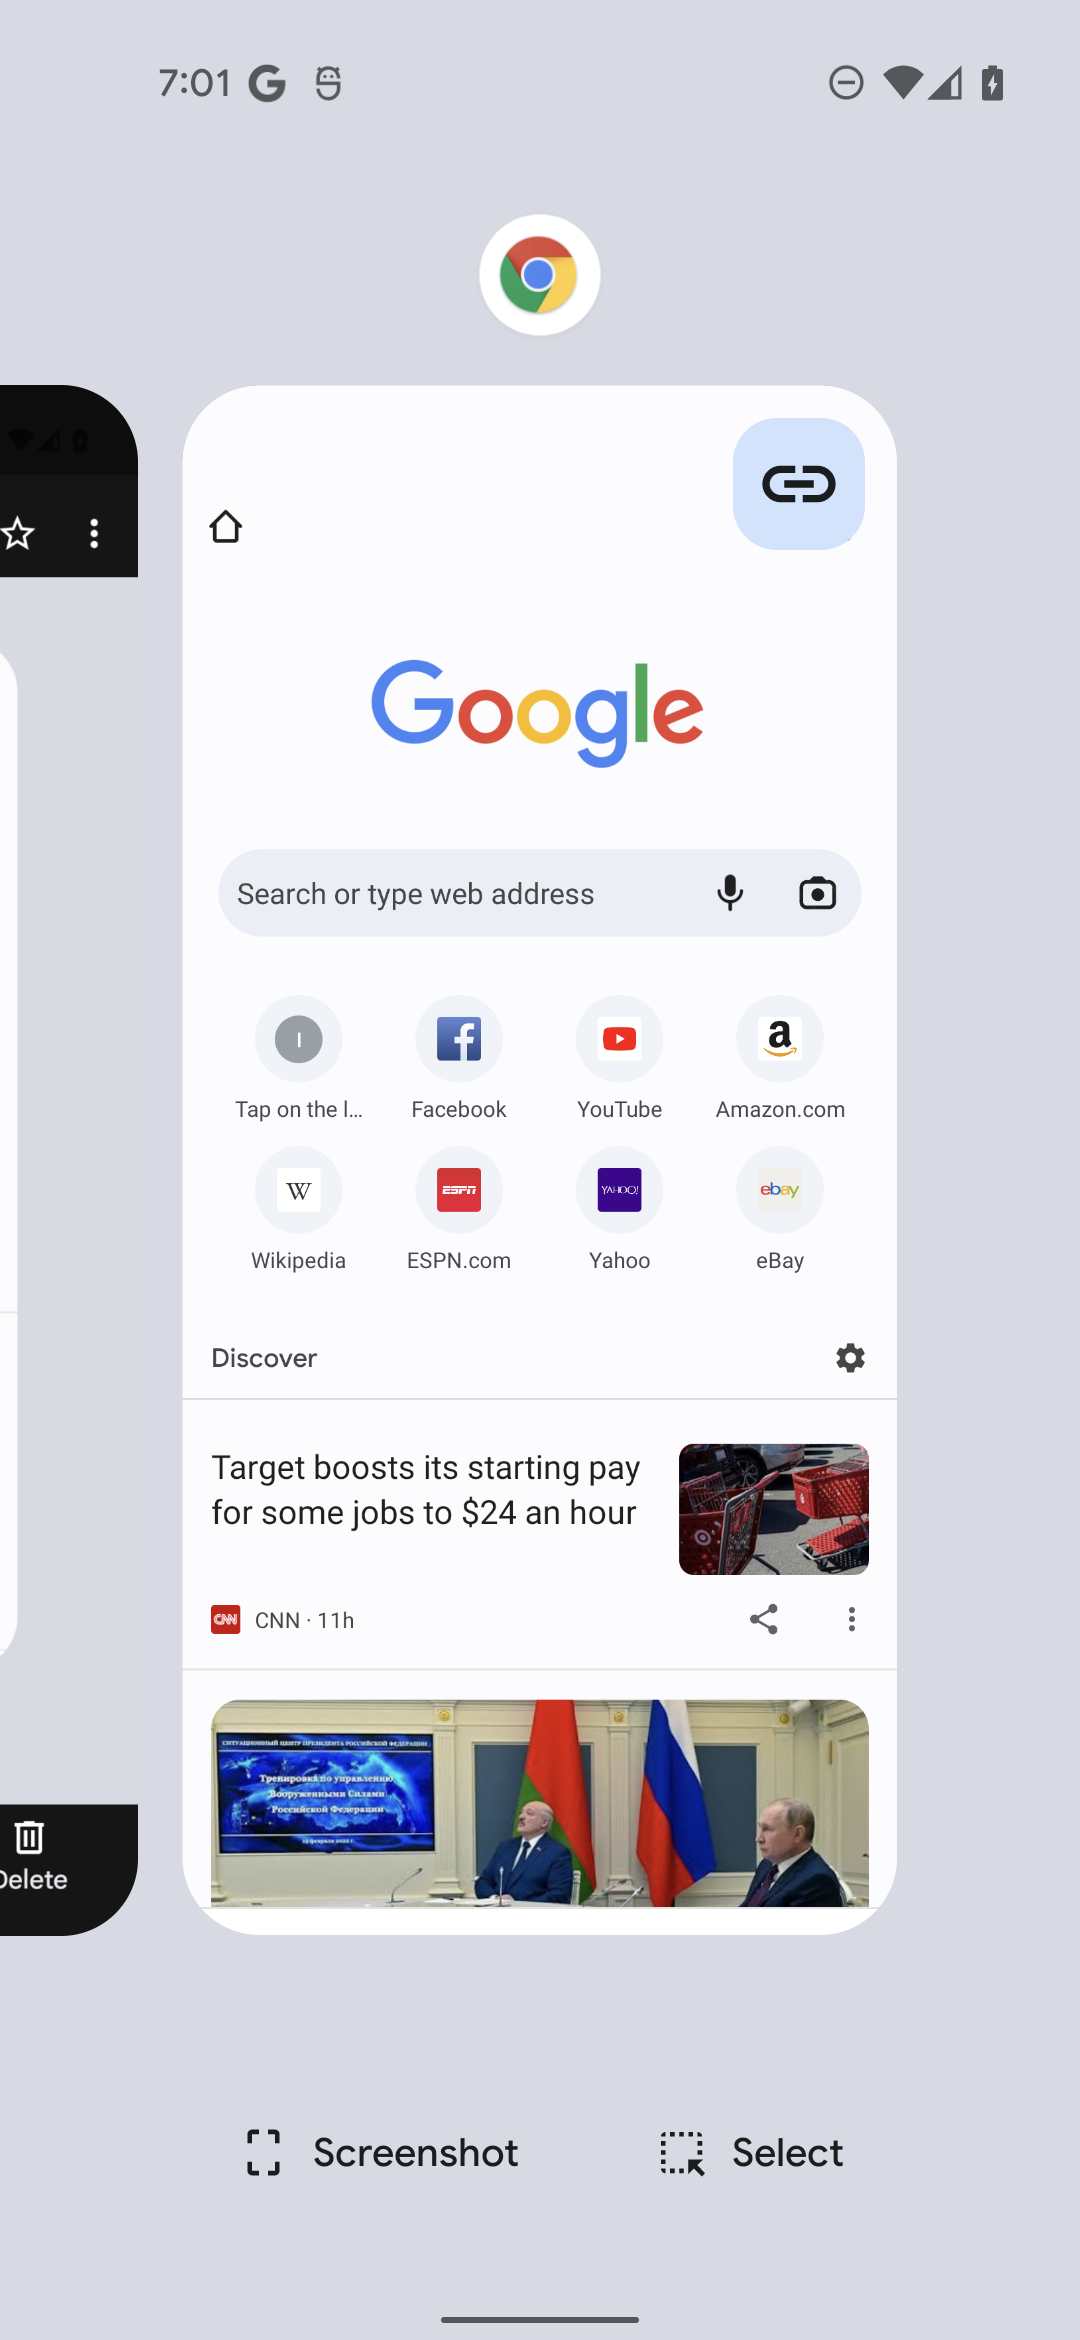
\includegraphics[width=0.3\columnwidth]{fig/recents-screen.pdf}
\caption[Recent Apps Screen Example]{A screenshot of Recents screen showing that Chrome is recently accessed. However, a spyware app will not appear in the recent screen (if it chooses to hide from the recent screen), despite that one of its Activities is recently created and displayed.}
\label{fig:recents_screen}
\end{figure}


\subsubsection{Mitigations}
For apps that seek to hide their icons, our recommendation is that Android should enforce stricter requirements on what apps can hide icons (e.g., the three requirements from Android 10 build r1 to r14 mentioned in footnote~\ref{footnote:hide_icon}).
Most apps that run on Android phones should be required to have an icon. In the case of exploiting TV app features, while we
understand that running apps with only \texttt{LEANBACK\_LAUNCHER} activities on
Android phones increases compatibility, such a feature leads to abuse as Spy24
has already demonstrated.

Launching apps by predetermined signal from another app is not only used for
malicious purposes but also for benign purposes (e.g., dial pad can be used for
testing and numerous benign apps use a browser link to open themselves).
While browser links can be easily tracked by examining the manifest, currently
users have no way to discover if apps can launch themselves with hidden codes.
The difficulty is in part because hidden codes are used dynamically during
runtime: the outgoing dialed number is sent to apps, and apps can freely decide
what actions to perform based on the number received. This design makes it hard
for the Android system to identify what hidden numbers are being tracked by each
app.  One possible mitigation is to allow users to review apps that can receive predetermined signals (e.g., a list of apps that listen for the
\texttt{NEW\_OUTGOING\_CALL} intent or have intent filters for specific browser links,
perhaps as part of the privacy dashboard).

One potential fix to stop apps from hiding from the Recents screen is to enforce
having at least one activity per app in the Recents screen.




\subsection{Persistence}
\label{subsec:persistence}
This section describes the methods used by spyware apps to persist on the target
device by obscuring the uninstallation process and creating ``diehard'' services
(automatically restarting themselves after stops and reboots).

%\subsubsection{Capabilities}

\subsubsection*{Capability \#7: Obscuring the Uninstallation Process}
\begin{figure}[t]
\centering
\includegraphics[width=0.6\columnwidth]{fig/DA_pdf.pdf}
\caption[Disabling Uninstall Buttons Example]{An example of an app disabling both the
Force Stop and Uninstall buttons on Android 6.}
\label{fig:da}
\end{figure}
One way to prevent users from stopping and uninstalling an app is by
disabling the Force Stop and Uninstall buttons (see
Figure~\ref{fig:da}).  For Android versions below 7.1,
these buttons can be disabled simply by registering the app with
\texttt{Device Administrator} (DA) privileges (as detailed in prior
work~\cite{shan2019device}). To enable these two buttons, the user
would have to deactivate the device administrator privileges for the
app.
%
Since Android 7.1, while the Force Stop button is disabled for DA
apps, the Uninstall button will remain enabled even if the app
registers as DA.  As a result, users can uninstall DA apps
directly~\cite{shan2019device}. Overall, I observe 11 apps that
register as DA.
%% \damon{this is really cryptic and difficult to
%% understand.}\alex{fixed}

Two apps, Cerberus and Mobile-tracker-free, directly interfere with the
uninstallation process, a behavior often observed in Android
malware~\cite{shan2019device,aljarrah2016maintaining}. Cerberus employs a series
of mechanisms to stop users from deactivating it as a DA app or
uninstalling it. These include trying to lock the device by invoking the
\texttt{lockNow} method of the \texttt{DevicePolicyManager} class and starting
an activity that blocks users from clicking on any buttons. Mobile-tracker-free,
on the other hand, tries to stop users from uninstalling it by starting an
Activity that blocks the uninstallation screen and requests a password set
by the abuser to proceed.

\subsubsection*{Capability \#8: Creating Diehard Services}
%\alex{a new title?}
%
Spyware apps strive to always be executing on the target device so
that they can collect as much information as possible.  I focus on
the ``diehard'' mechanisms that apps use to automatically restart
themselves after being stopped by the Android system (e.g., due to low memory) or after device
reboots. Echoing the diehard implementations discovered in prior
work~\cite{shao2019lightweight,zhou2020demystifying}, I observe two
main ways used by spyware apps to create diehard services. I also note
a third approach that appears to originate from the spyware ecosystem
and be a byproduct of other capabilities.

\textbf{Leveraging Scheduling Frameworks.} Scheduling frameworks such as Android's
\texttt{JobScheduler}~\cite{JobSched94:online} and
\texttt{AlarmManager}~\cite{AlarmMan39:online} enable apps to repeatedly
restart. Apps can schedule to be restarted either when they are
first started or when they are being terminated by the system. To schedule
themselves to be restarted shortly after they are terminated, they override the
\texttt{onDestory} function, which is called before the app is terminated by the
system.

\textbf{Monitoring System Broadcasts.} Monitoring system broadcasts offers another way to wake up apps if they are not running already. Android sends broadcasts when various system events occur~\cite{Broadcas25:online}, and apps that monitor these system broadcasts will be woken up if they are not running already. Table~\ref{tab:monitor_broadcast} lists various systems broadcasts and the number of apps that monitor them.\footnote{Only a small number system broadcasts can be used to wake up apps after the restrictions introduced in Android 8~\cite{Implicit72:online}. I only consider these system broadcasts.} The spyware apps in our study predominantly use the \texttt{BOOT\_COMPLETED} broadcast. Monitoring
\texttt{BOOT\_COMPLETED} allows spyware apps to restart themselves
after the device reboots: the Android system will send a
\texttt{BOOT\_COMPLETED} system broadcast upon reboot, and spyware apps that listen
for this broadcast will automatically restart themselves. While \texttt{NEW\_OUTGOING\_CALL} and \texttt{SMS\_RECEIVED} are also popular, I note that they serve dual purposes (\texttt{NEW\_OUTGOING\_CALL} can be used to launch a hidden app and \texttt{SMS\_RECEIVED} can be used to monitor SMS messages).

\textbf{Listening for Accessibility or Notification Events.} Apps that choose to register as an
\texttt{AccessibilityService} or
\texttt{NotificationListener- Service}
can also survive device
reboots. However, unlike the two techniques described above,
\texttt{AccessibilityService}
is less reliable because it can be
turned off by Android for battery saving reasons~\cite{AndroidA0:online,Accessib46:online}.


\begin{table}[t]
  \centering
  \begin{tabular}{lr}
    System Broadcast         &\# of Apps  \\
    \midrule
    BOOT\_COMPLETED          &10          \\
    SMS\_RECEIVED            &9           \\
    NEW\_OUTGOING\_CALL      &9           \\
    PHONE\_STATE             &6           \\
    ACL\_DISCONNECTED        &1           \\
    ACL\_CONNECTED           &1           \\
    LOCKED\_BOOT\_COMPLETED  &1           \\
    WAP\_PUSH\_RECEIVED      &1           \\
  \end{tabular}
  \caption{System broadcasts and the number of apps monitoring them.\label{tab:monitor_broadcast}}
%  \vspace*{-1cm}
\end{table}

\begin{facingcaption}{table}
\caption[Systematization of Commodity Spyware Vulnerabilities]{Systematization of commodity spyware vulnerabilities. Circles denote the severity level of the insecurity. \protect \partrating\ indicates at least one instance of the insecurity; \protect \rating{100} indicates all app functionality is insecure; * indicates URLs are temporary and expire.
          Shading added to improve readability.}
\label{tab:apps_spyware_vuln}
\renewcommand\tabularxcolumn[1]{>{\RaggedLeft\arraybackslash}p{#1}}
\parindent=0pt
\setbox0=\vbox{%
\vsize\textwidth
\hsize\textheight
\linewidth\hsize
\columnwidth\hsize
\textwidth\hsize
\textheight\vsize

\begin{tabular}{lm{2.5cm}m{2.5cm}m{4.2cm}m{2.9cm}m{3.0cm}}
%		\toprule
		Spyware Apps & Eavesdropping Sensitive PII & Cross-account Request Forgery & Unauthenticated Access to Victim Data & Poor Data Retention Practices & Unauthenticated SMS Commands \\
		\midrule
		mSPY & \partrating &  & Images &  &\\
		Mobile-tracker-free & & & Streaming & & \rating{100}\\
		Clevguard & \partrating & & Images* & &\\
\ltgrey 	HoverWatch & & & Audio* & &\\
\ltgrey 	Flexispy & \rating{100} & & Images/Audio* & &\\
\ltgrey		Spyic &  &  & Images* & \partrating &\\
		Spyhuman & & & Images/Audio & &\\
		TheTruthSpy & \rating{100} & \rating{100} & Images/Audio & \rating{100} &\\
		iKeyMonitor & & & & &\\
\ltgrey		Cerberus & & & Audio &  & \\
\ltgrey		Spy24 & & & Streaming* & &\\
\ltgrey		Spapp & & & Images/Audio/Streaming & \partrating & \rating{100}\\
		Meuspy & & & Images/Audio & \partrating &\\
		Highstermobile & & & Images &  &\\
%\ltgrey		LetMeSpy & & & & &\\
%		Spylive360 & & & Images/Audio & \rating{40} &\\
%		Talklog & & & & &\\
%		\bottomrule
	\end{tabular}


\singlespacing
}
\centerline{\rotatebox{90}{\box0}}
\end{facingcaption}


%% \geoff{so ``waking
%% up apps'' is just for surviving reboots?  I might want to rename}\alex{fixed.
%% techinically apps can be woken up in many ways...after being stopped. by
%% \texttt{BOOT\_COMPLETED} seems to solely used for waking up purposes}

%We also note that the old \texttt{camera} framework has an API called
%\texttt{getSupportedPreviewSizes}, which supplies a list of supported preview
%sizes\alex{not sure about camera2 framework}.

%While the API document s

\subsubsection{Mitigations}
Apps that seek to persist by registering as device administrator will
no longer be successful as users can uninstall them on most devices
running Android 7.1 or above. For apps that seek to interfere with the
uninstallation process by creating activities or locking the device,
past literature on malware defense~\cite{fernandes2016android,
  aljarrah2016maintaining} has suggested improving attack detection
and introducing system level support for detecting and reacting when
an app window is covered.
% \geoff{are there suggestions from the malware papers?}\alex{fixed}


Prior work~\cite{zhou2020demystifying} has investigated various ways
of creating diehard apps. According to the authors, the diehard
mechanisms I observe are very resilient and can only be effectively
stopped via a force stop.
%% \geoff{``the above abuses can only be effectively stopped'' --- by abuse do you
%% mean spyware activities in general, or just the methods for keeping apps
%% alive/waking up apps?}\alex{fixed}
%% However, it is unlikely that users would force stop instead of
%% uninstall a suspicious app after they have discovered it.
Additionally, the fact that many spyware apps register as device administrator
creates another layer of complication --- while apps registered as DA may be
uninstalled directly after Android 7.1, the force stop option is disabled,
making it difficult for users to stop the spyware apps (unless they uninstall
it).
However, even if apps prevent a force stop, users can still uninstall
them.
I also recommend adding a dashboard for monitoring apps that will automatically
start themselves.\footnote{We note that some Android phones (e.g., Xiaomi) have a
built-in dashboard for managing apps that can automatically start
themselves~\cite{HowtoDis42:online}.}

%\geoff{so...no mitigation then?}\alex{fixed}


% \subsection{Discussion}
% TBD


% Before diving into the actual implementation, I first detail the general
% process of building customized camera implementations. Each camera is in
% Android is a \texttt{CameraDevice} and is responsible for producing raw data
% frames~\cite{Cameraca74:online}. Apps receive these raw data frames by
% specifying an output  buffer, which for example could be a
% \texttt{SurfaceView}, \texttt{ImageReader}, \texttt{RenderScript.Allocation},
% or \texttt{TextureView}~\cite{Cameraca74:online}.

% In practice, I observed X different customized camera implementations: (1)
% through creating 1x1 pixel SurfaceView.

% To create a camera session, provide it with one or more output target buffers
% your app can write output frames to.

% The first implementation creates 1x1 pixel previews. It requires the
% \texttt{SYSTEM\_ALERT\_WINDOW} permission to draw over other apps.
% Applications

\section{Spyware User Data Protection}
\label{sec:data-leak}

%\damon{at a high level I need to make it clear that I only attempted to access our own data and I should also include citations to prior news articles and industry reports that overlap with our findings.}

%% \geoff{need to describe the various infrastructure elements involved
%%   (device, accounts, servers) and lifecycle steps (when does the
%%   abuser create/setup/access an account, does the abuser download and
%%   install the spyware on the victim's device after creating an
%%   account, abuser account registration vs victim device registration
%%   to an abuser's account, high-level of how the abuser remotely
%%   controls the spyware on the victim's device).  might also go earlier
%%   in the paper for context on app implementation, but particularly
%%   needed for understanding the data protection part.}
%\sumanth{Not sure where this should go. Here in the intro?} \geoff{yes put it here for now, don't
%  worry about the flow with other parts for now}

In this section I assess how well spyware apps secure the user data they exfiltrate and store.
For this assessment, in addition to the victim and the abuser, we
consider a third actor: an external attacker who seeks to undermine the
security of the spyware app.  The attacker's goal is to exploit any
integrity, authorization, and authentication issues with the spyware
app to access victim data as a third party.
% that the attacker is not supposed to have access to.

%% When discussing each of the security issues below, I note further
%% assumptions about the attacker that are specific to a particular
%% issue.

%% Table~\ref{tab:apps_spyware_vuln} summarizes the threats we
%% investigated and shows which apps are susceptible to them.

We start by describing our
methodology for investigating the data protection practices of the
spyware apps, and then discuss each of the vulnerabilities I uncovered (summarized in Table~\ref{tab:apps_spyware_vuln}).

\subsection{Methodology}
\label{subsec:experiemental_setup}

%\sumanth{Revised methodology section 4.1}
For each app I analyzed, I obtained an account (providing payment
information when necessary) and registered the app on a Pixel 2 XL
Android phone running Android 10.
%% I used man-in-the-middle (MITM) traffic inspection to perform our
%% network analysis on each spyware app.

To identify apps sending data from the device to the backend servers via unencrypted connections I used \texttt{tcpdump},
listening on a Windows 10 machine interface configured as a mobile
hotspot, to capture and inspect app traffic over the network.  We
configured the Android phone to connect to the PC and recorded all
traffic exchanged with the app servers, without any proxy in between
(avoiding any potential TLS handshake failures due to certificate
pinning).

To study the interactions between the spyware web portal interface and
the spyware backend servers, I used the open-source \texttt{MITMProxy} tool to
decrypt HTTPS traffic.  This configuration gave us access to
authentication tokens (session cookies, secrets, etc.) for conducting
forgery attacks on our test accounts.  I were able to login to all
portals without error (e.g., there were no issues with certificate
pinning).  I also analyzed the HTML content displayed via the spyware
web portal interface, extracting the URLs linked to uploaded user
media (images, audio, etc.).  I then performed a sequence of
experiments that tested and verified each insecurity listed in
Table~\ref{tab:apps_spyware_vuln}.

% I installed a trusted PEM certificate (generated
% by the proxy) on the phone, adding the certificate to the list of user
% store certificate authorities.

%% \geoff{could also aggregate the specific methodology parts from the
%%   subsections here}

%% For each app I analyzed, I obtained an account (providing payment information when necessary) and registered the app on a Pixel 2 XL Android phone running Android 10. I used a man-in-the-middle (MITM) traffic inspection approach to perform our network analysis on each spyware app, focusing on outgoing requests from each app that I manually installed on the Android phone. I leveraged the open-source MITMProxy tool to inspect outgoing requests, which I setup and ran on a Windows 10 PC noting its IP address. I then configured the Android phone to connect to a mobile hotspot setup on the PC, and configured a manual proxy to route all traffic to port 8080 - that the traffic inspector actively ran on. In order to decrypt TLS traffic, I installed a trusted PEM certificate (generated by the traffic inspector) on the phone, which adds the certificate to the list of user store certificate authorities. For each spyware app, I installed the mobile app onto the Android phone, logged in using the abusers credentials and ran through the sequence of experiments which test each insecurity listed in table \ref{tab:apps_spyware_vuln}.
%% I also analyzed the spyware web portal interface and extracted the path for uploaded user media (images, audio, etc) which I used for the following experiments.

\subsection{Results}

Table~\ref{tab:apps_spyware_vuln} summarizes the threats we
investigated and shows which apps are susceptible to them.
%
We describe each of the threats in turn, summarizing its context, its
associated threat model, any additional methods I employed, and the
specific results I discovered for the vulnerable apps.

%% I start by briefly describing each insecurity, along with the threat
%% model and experimental setup used to identify the insecurity. I then
%% discuss a subset of the apps which demonstrate each insecurity. To
%% structure our analysis, I focused on security mechanisms for
%% protecting sensitive user data.

%We are less interested in flows that do not aid in compromising the app or user data; for example, apps that are using unsecured HTTP connections for non-sensitive functionality.

%% \geoff{the structure of these subsections results in some redundancy
%%   across the various parts, which is not ideal.  but it does have the
%%   virtue of being explicit about each of the parts.}

%\subsubsection*{Insecurity \#1: Submitting sensitive victim or abuser PII over the network}
\subsubsection*{Insecurity \#1: Eavesdropping Sensitive Personally Identifiable Information (PII)}
%\subsubsection{Eavesdropping sensitive PII}

Some spyware apps transmit highly sensitive victim data, such as photos,
texts, and location, from the victim device to the spyware backend
servers using unencrypted HTTP connections.  A MITM attacker who
eavesdrops on the same communication channel (e.g., same WiFi network)
could collect all data and credentials sent unencrypted
over the network.  Furthermore, credentials leaked over the network enable
an attacker to login to the abuser's account and gain access to all of
the victim's data exfiltrated by the spyware.

\textbf{Threat Model.} I assume that the attacker can eavesdrop on
all messages sent by the mobile device infected with spyware (e.g.,
the attacker uses the same WiFi network as the victim, and the WiFi
network is not using link-layer encryption).

%% I also assume that the network used when eavesdropping is unencrypted
%% (e.g., a WiFi network not using link-layer encryption).

%% \geoff{doesn't the WiFi network need to
%%   be unencrypted (not use link-layer encryption)?} \sumanth{Addressed}

\textbf{Experimental Setup.}
%% To uncover sensitive data flows, I utilized the spyware's
%% functionality and observed the outgoing network traffic from the
%% target device.
We filtered the captured traffic to observe network activity from each app over
insecure channels like HTTP, and used a combination of search and
manual inspection to analyze the recorded traffic for sensitive data
such as leaked credentials (user names, email addresses, passwords),
text messages,
% call logs,
etc.

%% Filter's were setup to flag any network activity over insecure
%% channels like HTTP. These packets were manually analyzed to see if
%% they leaked passwords, messages, call logs, etc. Similarly I flagged
%% packets containing sensitive PII's (i.e., user/abuser email) using
%% regex matching.

%% \damon{did I check for password, sms, call logs, messages?}
%% \sumanth{Added a line above that I analyzed insecure packets to see
%%   if they leaked all these.}

\textbf{Results.}  Four spyware apps in our study leak at least some
of their data using vulnerable communication channels.  TheTruthSpy
submits all of its data over HTTP, and it leaks the abuser's
credentials for TheTruthSpy servers (abuser email address and
password) in the authentication request during app setup.
%% It also leaks the abuser email address
%% in response to an unauthenticated request for registration information.
%% TheTruthSpy also leaks the abuser's email address in the response to
%% an endpoint called during setup time.
%% \geoff{victim's?}
%% \sumanth{Edited to make it clearer. There are 2 cases - email and pwd
%%   leaked in a request during setup time, and just the email leaked in
%%   the response every time a particular endpoint is called}.
%% \geoff{``endpoint'' is still a bit vague? if the email address leak is
%%   also during setup, then I think I can leave it out (the full
%%   credential leak is already a worse case)}
mSPY leaks only
the upload path for its images in an HTTP response back to the
victim's device when the image upload succeeds.
%\sumanth{Added this for Clevguard}
Clevguard uploads its images over HTTP, making it is possible for an attacker to reconstruct the image from the payload.  Flexispy uses
HTTP for all of its communication, but it implements a custom
encryption protocol for the data it sends.  However, a previously
discovered flaw in Flexispy's encryption makes it possible to
intercept personal data sent over the
network~\cite{Stalking85:online}.

%% I observed 3 spyware apps send their data - like texts, images,
%% locations - over plain HTTP protocol. \textbf{TheTruthSpy} submits all
%% its data over HTTP. Further, it leaks both the abuser email and
%% password during app setup time (when authenticating), and the abuser's
%% email during setup time. \textbf{mSpy} on the other hand leaks only
%% the upload path for its images in a HTTP response back to the victim's
%% device once the upload is successful. While both these apps send data
%% in the clear, \textbf{Flexispy} implements a custom encryption
%% protocol even though it sends data over HTTP. However, a perviously
%% discovered flaw in Flexispy's encryption makes it possible to
%% intercept personal data being sent over the network
%% \cite{Stalking85:online}.

\subsubsection*{Insecurity \#2: Cross-account Request Forgery}
%\subsubsection{Cross-account request forgery}

Knowing a particular user identifier, or a file path that provides access to images, audio, or video on the server, an attacker can use valid
cookies from one spyware account to access data or perform actions in
the accounts of other spyware users.

\textbf{Threat Model.} The attacker can register a spyware account and
log into it. Using a MITM traffic inspector (similar to our proxy
described in Section~\ref{subsec:experiemental_setup}), an attacker
can intercept and replay authenticated requests from their account. We
assume the attacker knows the ID of the targeted user's account ---
either through enumeration, or from the ID being leaked over the
network or in a public data dump~\cite{mSpybrea38:online,
  Companyt8:online, HackerSt66:online, Cerberus12:online,
  Stalkerw59:online}.

%% \damon{this is cryptic, I would suggest directly stating that the
%%   attacker can register/purchase a spyware account and log into it.}
%% \geoff{still cryptic :-) \sumanth{Reworked this section. Hope its
%%     better now :)}}

\textbf{Experimental Setup.} I used two accounts for each app, one
for the attacker and the other as the targeted spyware user.  I then
recorded and replayed authenticated requests from the attacker's
account to the targeted user's account, substituting the ID of the
targeted user's account in the requests without changing authorization
tokens provided by the attacker's account (e.g., session IDs, API
keys).  I only replayed requests to our test accounts, and
made no attempt to access content belonging to any other account.

%% \sumanth{Reworked based on Damon's feedback}\damon{this need to be
%%   improved to better describe that I had two accounts and that we
%%   checked for cross-account data leakage. I should also be clear that
%%   I only probed our own accounts and I did not attempt to access any
%%   content that potentially belonged to another person's account.}

\textbf{Results.}  Only one of the apps in our study is vulnerable to
cross-account request forgery.
%% I disregarded apps which have API
%% structures with no IDs that identify users or devices, and instead
%% rely solely on session IDs for authentication and
%% identification.
%% \sumanth{Added this to tie well with results in table}
%% \geoff{I'm still not sure the distinction between ``No'' and ``--'' in
%%   the table.  does ``--'' mean that by design the app is not
%%   suscectiple to CARF?  and No means that the app's design could be
%%   susceptiple but its implementation is correct?} \sumanth{Yes, exactly!}
With TheTruthSpy, it was possible to
access all data (messages, contacts, locations, images, etc.)  in the
targeted account using a cookie provided by the attacker's account,
and simply swapping the attacker's device ID with the targeted
account's device ID in requests to TheTruthSpy server.  Furthermore,
when I registered multiple test accounts in succession, I noticed
that the device ID that TheTruthSpy assigns to a new device is a six-digit
integer which increases incrementally when new devices are registered.
%% \damon{how did I determine that it increased
%%   incrementally?}\sumanth{I see newer accounts always get assigned
%%   higher numbers which are very close by to older ones. I tested with
%%   2 accounts and found the deviceIDs were close by.}
The combination of insecure access controls across accounts and
predictable device IDs makes it possible for an attacker to retrieve
data from other accounts without needing to identify the device ID
beforehand.

%% by swapping the
%% device ID of a target account, while using valid cookies provided by
%% the first account. Furthermore, the device ID TheTruthSpy assigns to a
%% new device is a 6 digit integer which increases incrementally when new
%% devices are registered. \damon{how did I determine that it increased
%%   incrementally?}\sumanth{I see newer accounts always get assigned
%%   higher numbers which are very close by to older ones. I tested with
%%   2 accounts and found the deviceIDs were close by.} The combination
%% of insecure access controls across accounts and predictable device ID
%% makes it possible for an attacker to retrieve data from other accounts
%% without needed to know the device ID beforehand.

% \sumanth{TODO: Any other CARF in other apps?}

%\subsubsection*{Insecurity \#3: Leaking sensitive data on public server URIs}
\subsubsection*{Insecurity \#3: Unauthenticated Access to Victim Data}
%\subsubsection{Unauthenticated access to victim data}
\label{sec:leaky-urls}

%% \geoff{would be good to describe the scenario: some apps use CDNs or
%%   backend servers to store media data (do I know why? cost?), and the
%%   URLs they generate to the media data are unauthenticated.  the idea
%%   is to note the distinction between URLs to content on the app's server
%%   vs URLs to media stored on different infrastructure (which is my
%%   understanding of what's going on here, which may be wrong?)  either
%%   way, I want to give some sense/intuition for why URLs for accessing
%%   this content is different than other content stored on the spyware
%%   servers.} \sumanth{Good point! I've added this in the intro of the section below. One thing missing might be the reasoning as to why they choose to store media on different servers. Cost might be the main reason yes.)} \geoff{thanks, edited}

Many of the spyware apps use different backend infrastructure to store
and deliver media data that is distinct from the servers that
abusers use to access the app dashboard (e.g., abusers login
to the dashboard via the website domain in Table~\ref{tab:apps_selected}, but
the app may use a CDN to deliver images and videos).
This separate infrastructure
includes cloud storage (e.g., AWS S3 buckets), content distribution
networks, and other shared hosting services, all of which are
presumably cheaper to use for serving media data.
% I observed that
Some of the spyware apps are less careful about protecting the
data that they store on this hosting infrastructure, often allowing
unauthenticated access to the URLs they generate to stored media data.
Further, I observed user data stored in predictable URLs that make it
possible to access data across different accounts, protected solely
through security by obscurity and vulnerable to enumeration. Table~\ref{tab:apps_spyware_vuln} lists
the kinds of data leaked in public URLs for the apps studied. Failure
to authenticate access to user media (images, audio, etc.) using
mechanisms like cookies is a common example of this category of
vulnerability.

\textbf{Threat Model.} I assume that the attacker has knowledge of
the media upload path for the app based on studying media paths
revealed using accounts owned by the attacker.  For apps that use the
device ID in URL path components, I also assume the attacker knows
the targeted device ID.

\textbf{Experimental Setup.} To discover sensitive data leakage, we
focused primarily on URLs used to store media artifacts (images,
audio, video, etc.).  I extracted these URLs by examining the
browser-generated HTML content when accessing the dashboard in the
spyware account.  I only attempted to access media upload paths from
our test accounts, and made no attempt to access content belonging to
any other account.

%% \geoff{how did you collect URIs using the attacker's account?}
%% \sumanth{Addressed. Also added another statement to make sure I are
%%   clear that I collected media links from our own accounts}

\textbf{Results.}  Six of the apps in our study store their data in
public URLs accessible without authenticated access.  I disregarded
apps which store data in URLs that, although public, expire after a
short duration (e.g., Spyic's links to images expire after 1,800
seconds).

% I also disregard those apps which required authenticated
%(cookie-based) access to data. \geoff{not sure the distinction between
%  this case and other authenticated account access?}

Highstermobile stores its images with a URL scheme as a concatenation
of the image upload timestamp (UNIX timestamp with seconds precision)
and a double digit random number, with no other per-device ID in the
path (e.g.,
\texttt{\url{https://domain.com/path/photo_<timestamp><00-99>.png}}).
% \sumanth{\url{https://evt17.com/iphone/uploads/gallery/image/thumb/photo_<UNIXTimestamp><00-99>.png}}.
Since an attacker could plausibly iterate over a short range of
timestamps and random digits, this naming scheme makes it
straightforward for an attacker to gain unauthorized access to media
stored on the server for other accounts.

Cerberus and Spyhuman use public URLs that are a combination of device
ID and Unix timestamp
% (also Unix timestamp with seconds precision)
(e.g., \texttt{\url{https://domain.com/<DeviceID>-<timestamp>.ext}}).
While both of them require the attacker to know the device ID before
hand, an attacker could for instance obtain the device ID from data
dumps made public in breach attacks~\cite{mSpybrea38:online,
  Companyt8:online, HackerSt66:online, Cerberus12:online,
  Stalkerw59:online} or with physical access to the device.
%% \geoff{I added this, are there better scenarios?} \sumanth{Maybe also
%%   from public data dumps which have device metadata?}
Cerberus stores audio insecurely using the device IMEI as the device
ID.  Spyhuman stores both its images and audio insecurely using the
Android serial number as its device ID.  With both apps, an attacker
knowing the device ID could plausibly iterate over a short range of
timestamps to retrieve data stored on the server.

% \url{https://www.cerberusapp.com/audio/<DeviceID>-<UNIXTimestamp>.mp4}
% \url{https://dwnlnew.webdown2.com/rec/<DeviceID>/<UNIXTimestamp>/file.mp3}

Three other apps store data on servers using public URLs that rely on
security through obscurity, but they generate URLs that are neither
enumerable or predictable.  For instance, Spy24 allows WebRTC remote
streaming through a public URL based on a request ID generated by the
app, Spapp requires two alphanumeric keys to access image and audio
files on the server, and Meuspy generates unguessable URLs to
store images and audio.  Although certainly not good security
practice, the risk associated with unauthenticated access is lower
than for the other apps I discussed.

%% these three apps do not implement
%% good security practice by solely depending on security by obscurity,

%% \geoff{conclusion?  not good security
%%   practice but lower risk than the other apps?} \sumanth{Added.}

% complicated

%% Among the other 3 apps which leaked data on public server, all of them generate URIs which although public, is neither enumerable or predictable. These rely solely on Security through obscurity. \sumanth{e.g \textbf{Spy24.app} (which allows WebRTC remote streaming through a public URL based on a request ID generated by the app), \textbf{Spapp} (which requires 2 alphanumeric keys to access any image/audio on the server) and \textbf{Spylive360} (which generates complicated URLs to store images/audio)}

\subsubsection*{Insecurity \#4: Poor Data Retention Practices}
%\subsubsection{Poor data retention practices}

%% \sumanth{I rewrote this section to better explain what I had in mind.}

Some spyware apps have poor data retention practices that prevent
victim data from being deleted from the spyware servers. These data retention issues pose serious security and privacy risks~\cite{santhanam2022scraping}. A data breach could expose residual victim PII which has persisted even if, for instance, the abuser has deleted their account.

%% , in some cases because the data is either unaccessible by the abuser
%% or unassociated with any account.



%% All there of these cases involve unauthorized transmission of data which remains on the server indefinitely, and is either unaccessible by the abuser or unassociated with any account. These scenarios poses a risk if a data-breach exposes residual victim/attacker PII which has continued to persist.

%% \geoff{if I just have one app that has all of these risks, then we'll
%%   want to rework the story a bit}

%% Again, all data uploaded in both of these cases has the potential to
%% be leaked in a data breach.

%% \sumanth{I rewrote this section to better explain what I had in mind. Broadly speaking there are 3 cases here - Unassociated data sent without logging in, data sent but inaccessible without purchase, data sent after license expires or app is deleted. I've moved the part of 'delete' not actually deleting data to the end of section 4 along with the other misc stuff.}

%\geoff{who installed the app but never
%  used it?  an abuser who decided not to use it?  is this a compelling
%  risk?}

%% \geoff{do the apps provide the capability for the abuser to delete
%%   uploaded victim data via their server account?  if so, did I test
%%   to see if that data is actually deleted?  if not, there might not be
%%   time to do it for the submission, but is something to add for later} \sumanth{Yes, for apps which allowed the delete account option, I tried to see if both uploaded media and replaying endpoints to get, and have results for this}

%% Some apps send user data (like text messages, images, keylogger activity) to the spyware app servers before the abuser logs in/sets up the account. In some cases, this data is never visible to the attacker but is stored on the server. In some cases, user data (like images, audios, text messages, etc) persists even after explicitly deleting the account associated with the abuser. Further, in the event the license expires some spyware apps continue to send data to the backend servers, unaware of the expired license. This poses a particular issue if a data-breach exposes sensitive user data of victim's, who might have installed but never used the app \cite{esetandr4:online}

\textbf{Threat Model.} Data uploaded to the spyware servers and never deleted poses a long-term risk to being made public in data dumps associated with breach attacks.
%\sumanth{I'm not sure if this has a threat model because this doesn't have an attacker per say.}
% \geoff{data never deleted poses long-term risk to data breaches?} \sumanth{Added.}

\textbf{Experimental Setup.}  To discover poor data retention practices, I analyzed network traffic generated after the app license expired, but with the victim device still logged in.  I also tested
access to media on deleted accounts using their public URLs up to
seven days after deletion of the account.
%\sumanth{Added this line.}

%% Network traffic from the target device was captured and analyzed
%% before the abuser logged in and after the license expired.  Data
%% uploaded to the server was tested for persistence after the account
%% was expired.

\textbf{Results.}  Four of the apps in our study demonstrate poor data retention practices.

Consistent with its other data vulnerabilities,
TheTruthSpy also has data retention issues.
% \sumanth{Based off of reviewer C's comments, I omitted the data sent before registration result here. I now only talk about the data sent after license expiry and data retained after account deletion.}
It continues to send
data from the victim's phone (e.g., text messages, images, keylogger
activity) to its servers after the app license expires. Further, it persists some data after the abuser
deletes their spyware portal account and the data associated with it.
%
%before the abuser even sets up their account.
%The exfiltrated data is never associated with an account and thus
%cannot be deleted even after logging in to the spyware portal.
%
%% \geoff{how is the exfiltrated data associated with the account if it
%%   is sent before the account is set up?} \sumanth{Clarified}
%% \geoff{who installed the app but never used it?  an abuser who decided
%%   not to use it?  is this a compelling risk?}
%It also continues to exfiltrate data to its servers after the app license expires.
In particular, images uploaded from the victim device persist after
account deletion, and the images remained accessible through the
public URLs used to access them (Section~\ref{sec:leaky-urls}).

%% abuser does not uninstall the logged-in app \sumanth{This seems like a
%%   common scenario abusers might do} \geoff{it does.  have we
%%   systematically tested what happens across the apps when I delete
%%   the portal account but leave the app on the device?} \sumanth{TLDR - I did capture traffic for this scenario, but the results are fuzzy, so I can omit this.}

%% Similarly, the exfiltrated data continues to be uploaded even after the abuser deletes their account, but does not uninstall the logged-in app \sumanth{This seems like a common scenario abusers  might do} or even in case the app license expires. The uploaded data, even though valid, is no longer accessible by the abuser.

Spyic has a data retention issue resulting from its trial usage
model.  When installed for trial use, Spyic uploads data from the
victim device to the server.  But it only allows access to its portal
after the abuser has purchased a subscription.  If the abuser decides
not to purchase the spyware, victim data persists indefinitely on
Spyic's servers (presumably in anticipation of the spyware user
eventually deciding to pay for a license).

%% \geoff{I added this statement, is it accurate?  do I think that
%%   Spyzie will retain the data indefinitely in anticipation of someone
%%   eventually paying?}
%% \sumanth{Yes, afaik there's no option to delete
%%   data on Spyzie.io. https://spyzie.io/privacy.html says you can go do
%%   so after loggin in (but there's no option on the portal to do this)
%%   or contact them to delete your data}

%\sumanth{TODO: Mention about results in table 5 e.g for apps like Highster Mobile.}
Lastly, both Spapp and Meuspy persist data from an abuser's account after deletion. Images in particular continue to be accessible through the public URLs used to access them.
% Lastly, Highstermobile also transmits data from the victim's device to its server before the abuser has signed in to the app.

%% Some logged-in apps continue to upload data to the server, but do not allow access to the data from the web portal until the abuser has purchased a valid subscription. However, if the abuser discards the app and forgets to uninstall it, the user data continues to be uploaded to the server.

%% Some of the apps in the study provide the capability for abuser to delete the account and data associated with it. However, some spyware servers do not actually delete the data already uploaded to the server from the victim's device. In TheTruthSpy, images
%% uploaded from the victim device persisted even after deleting the abuser account, and remained accessible through the public URLs used to access them.

%% abusers might delete their account but never uninstall the app from
%% the victim device, and the app might continue to upload data even
%% though it is no longer accessible by the abuser.

%% It sends data from the victim device before the abuser registers an
%% account (and this data is never accessible), and it sends data from
%% the victim device even after deleting the abuser account.

%% I observe both types of unauthorized transmission
%% in \textbf{theTruthSPy} - data sent before registering an account (and
%% never accessible), and data sent from the registered target device
%% after deleting the abuser account. Further, the user-uploaded images
%% did persist (and accessible through their links) even after the
%% abuser's account was deleted.

%\sumanth{One thing I might have to do again, is to verify if the unauthorized transmission PRE/POST for most apps. The data collected is a bit fuzzy for this, especially when all communication is over HTTPS it's hard to know if the app is transmitting unauthorized data or not}

%% \geoff{conclusions and implications?  victim data remains on spyware
%%   servers indefinitely, e.g., further exposing it to breaches?} \sumanth{Added in intro to this insecurity.}

\subsubsection*{Insecurity \#5: Unauthenticated SMS Commands}
%\subsubsection{Unauthenticated SMS commands}

Four of the spyware apps I studied accept commands in
the form of SMS messages.  This capability enables the abuser to
control the spyware app on the victim device even if it is
disconnected from the Internet, or as a secondary form of control to
the web portal accessible via the abuser's account.
%% \footnote{After Android 4.4, a third-party app can no intercept and delete SMS, and prevent it from being displayed in the chat \cite{SMSInterceptAndroidKitkat:online}.
%\geoff{if I mention this in the reverse-engineering section, then I can refer back to it there} \sumanth{Modified}
%\sumanth{This seems a bit out of context here. I vote to omit it}
%}

\textbf{Threat Model.} I assume that the attacker knows the phone
number of the target device (or can enumerate it). I also assume that
the attacker knows the list of commands available by referencing online
app documentation for SMS commands, such as~\cite{SpappSMSCommands:online,
  FlexispySMSCommands:online}.
%% \sumanth{I removed the password
%%   knowledge requirement. And added another assumption about the
%%   attacker's knowledge of available SMS commands}
%\damon{Can the attacker just log into the backend website if they know the password? I might have to pair back this attacker's knowledge.} \sumanth{Good point. I believe I can assume only that the attacker knows the phone number and nothing else.}

\textbf{Experimental Setup.}
% The spyware apps that support this capability provide a list of SMS commands on their website \cite{SpappSMSCommands:online, FlexispySMSCommands:online}.
%% \geoff{if an app has a list openly accessible, I could ref a URL to a
%%   page; a reader might be curious to see what the commands look
%%   like}.\sumanth{Added this in the Threat model section.}
For each app, I systematically tested their SMS commands on our test
device, focusing in particular on their method of authenticating commands. 
%, and execute the action after authentication.
%\sumanth{Added this line}

\textbf{Results.}  Two of the four apps that accept SMS commands
require a strong password or license key to authenticate SMS commands,
and so I disregarded them from further analysis.
The remaining two apps fail to check if the text message is from an
authorized sender, and execute the commands regardless.

% I commented this out since it didn't look like it referred
% specifically to the two apps discussed in our results (GV)
%% (some apps even execute the commands after the app license has
%% expired~\cite{esetandr4:online}).

%% \sumanth{Thanks folks! I realized I don't have 5 apps anymore and jut 4 - since I removed Talklog. Which means the other two apps which I have discarded are Cerberus and FlexiSpy - both of these require a password or a license key for authenticating their SMS messages. I moved this down to results and tweaked the above statements.}

% \grant{This last sentence seems to contradict the results section below, which states that only two apps are vulnerable to the attack?}
% \geoff{I think it should be two as well...Sumanth, can you confirm?}

Spapp executes highly-sensitive SMS commands, such as remotely wiping
the victim's phone, effectively unauthenticated.  During app setup,
the app generates a random two-digit number that serves as a passcode,
and only allows SMS commands that include the correct passcode to
execute on the device.  However, this simple passcode provides little
security since a methodical attacker can send redundant commands
enumerating all possible passcodes.

Mobile-tracker-free authenticates its SMS commands, but uses a default
constant as its password.  Unless the abuser explicitly changes this
SMS password, an attacker can successfully send commands using the
default.  However, the set of commands it supports via SMS is more
restricted than Spapp (e.g., the
command \texttt{MobileTrackerFreeSMS--getlocation}
returns device location information in an SMS response).

%Cerberus authenticates the SMS message and requires a
%plain-text password to be present in every SMS
%command (the password used to authenticate SMS message is the
%same one used to log into the abuser's Cerberus web portal). Similarly, Flexispy requires the license key of the abuser's account to be present in the SMS command.
%\geoff{did not edit since I might drop the ones requiring effective
%	passwords}

%% Among the apps which receive SMS commands, \textbf{Cerberus} authenticates the SMS message and requires a password (in plain text) to be present as the prefix of every SMS command. Further, the password used to authenticate SMS message is the same one used to log into the abuser's Cerberus web portal. Unlike Cerberus, \textbf{Spapp} doesn't authenticate the SMS commands it receives, and executes them regardless. The app allows highly sensitive SMS commands- like remote wiping the target phone - to execute unauthenticated. During app setup, the app appends a random 2 digit number at the end of each SMS command (\sumanth{maybe to offer some security?}), but this is not a viable solution to thwart a dedicated attacker. Much like Cerberus, \textbf{Mobile-tracker-free} authenticates its SMS commands, but uses a default constant as its password (which isn't changed unless done so explicitly by the user). However, the list of commands it provides is more restricted (e.g MobileTrackerFreeSMS--getlocation to get target device location information), and it doesn't allow execution of powerful commands like Spapp.

%\sumanth{An attacker can go through the phone number space and ping numbers to identify which device has the app installed based off its response. How can I add this?}
%\geoff{the second part (which device has the app installed)  seems a separate topic from Spapp sending SMS responses?}

%% \sumanth{Where should the below paragraph go?}
%% \geoff{I don't see a good place for the default password issue,
%%   so my suggestion is that I comment it out.  the one place
%%   where it might find a home is as an aside at the end of the results
%%   for CARF, but it would be a tangent.}

%% Three of the apps I studied generate weak default passwords for
%% abuser accounts.  If the abuser does not change the default password,
%% their account remains susceptible to brute-force attacks by a
%% determined attacker seeking to gain access.
%% %% \geoff{is this fundamental (all FlexiSpy passwords can only be six
%% %%   digits), or just an artifact of the default (the abuser can = the
%% %%   password to a much longer one)?} \sumanth{This is just an artifact
%% %%   of the default password.}
%% The Flexispy default password is just a 6-digit number.  The
%% iKeyMonitor default password is an 8-character string, with the first 7
%% characters being numbers and the last an alphabetic character.  The
%% Highstermobile default password is an 8-character alphanumeric string
%% containing lowercase letters.

%% \sumanth{Should I talk more about this? Check if they are
%%   brute-forceable, if the API has rate limiting? Max-retry policy?
%%   etc?}

%% Around 3 of the apps I studied generated weak/poor default passwords
%% for abuser accounts. These credentials are make it easy for an
%% attacker to break into and gain access to. \textbf{FlexiSpy} default
%% password is a just a 6 digit number. \textbf{iKeyMonitor} default
%% password is a 8 character string with the first 7 characters being
%% numbers and the last an alphabet. \textbf{Highster Mobile} default
%% password is an 8 character alphanumeric string containing lowercase
%% letters and numbers. \sumanth{Should I talk more about this? Check if
%%   they are brute-forceable, if the API has rate limiting? Max-retry
%%   policy? etc?}

%For one of the apps I studied, it was possible to access all of its
%features without payment.  Due to improper access control checks,
%one can can get around the payment restriction enforced by Spyzie.io (and all the apps belonging to its family).
%Spyzie.io doesn't display the abuser's web portal until the abuser has purchased a license. However, by creating a trial account and calling the endpoints (previously documented when using the premium account) to fetch the uploaded data from the server (like sms, location, etc), the accurate data is returned. This implies that while Spyzie.io denies access to the web portal until the abuser has purchased a license, their API endpoints do no such verification checks. It might thus be possible to create a mock website calling all of spyzie's endpoints to recreate the its dashboard. \geoff{not sure what
%  you mean here, can you describe a bit more?} \sumanth{Explained in detail}
%\geoff{ok...the complexity here may not be worth trying to explain it, and
 % I haven't even described the privacy risk (data uploaded via the trial
%cannot be deleted?  or does Spyzie have reasonable delete policies?)}

%\subsection{Discussion}
\subsection{Disclosure}
\label{sec:disclosure}

We disclosed the findings in this section to all the affected
vendors on June 14th, 2022. No vendor has replied to our disclosures as of the date of
publication (three months after our disclosure).


\section{Related Work}
\label{sec:related_work}
There exists a rich literature from both academia and industry that
examines various aspects of spyware apps (e.g., their usage in the
context of intimate partner violence).

Most related to our work, several prior studies have examined
the technical capabilities of spyware apps, including
both industry reports~\cite{PowerPoi79:online, SpyvsSpy59:online,
  ANewWave1:online, Whyyoush17:online, ReverseE12:online,
  YourInfo19:online, Stalking85:online, FlexSpyA1:online,
  diskurse89:online, VB2019Za6:online, SpywareP46:online, Androida91:online} and academic
papers~\cite{parsons2019predator, harkin2019consumer,
  harkin2020commodification, pierazzi2020data,
  feal2020angel,harkin2021operating}. However, many of these
efforts focus on documenting the functionalities supported by the
spyware apps and do not shed light on the implementation used to achieve
different functionalities (mostly because they focus on other facets instead
of the technical implementation challenges). The ones~\cite{Whyyoush17:online,ReverseE12:online,Stalking85:online,FlexSpyA1:online,diskurse89:online,VB2019Za6:online,parsons2019predator} that do study the implementation,
either examined only one or two apps or a small subset of the
mechanisms employed. Our work builds on these studies by systematically and comprehensively analyzing the underlying technical methods that apps employ to acquire different spying capabilities.

Also related, but orthogonal, is work focused on identifying and
detecting spyware apps, both industrial reports listing such
apps~\cite{Tekstalk86:online, esetandr4:online, ch33r10S37:online} and
academic efforts to characterize and build detection algorithms for
them~\cite{almansoori2022global,pierazzi2020data, chatterjee2018spyware, han2021towards,
  saroiu2004measurement, egele2007dynamic, roundy2020many,
  wang2006netspy, moshchuk2006crawler, randall2020trufflehunter}.  Yet
another related body of work examines spyware apps' presence in
different contexts such as intimate partner violence and
cyberstalking~\cite{havron2019clinical,freed2019my,tseng2020tools,thomas2021sok,freed2018stalker,fraser2010new,
  shimizu2013domestic,woodlock2017abuse,southworth2005high,southworth2006technology,dragiewicz2019domestic,mayrhofer2021android,motherboardstalkerwaremarket}.
I believe our findings, particularly characterizing the data access
mechanisms used by spyware, will be of use to those implementing
detectors, but detection is not itself a goal of our work.


Outside the context of spyware, another related research
domain has focused on how various kinds of malware (including spyware)
can abuse Android APIs to achieve abusive functionality.  In
particular, several papers have also identified abuse of the Android
Accessibility APIs, starting with Kraunelis et
al.~\cite{kraunelis2013malware}.  Following this line of work,
Fratantonio et al.~\cite{fratantonio2017cloak}, Kalysch et
al.~\cite{kalysch2018android}, Diao et al.~\cite{diao2019kindness},
and Naseri et al.~\cite{naseri2019accessileaks} have documented how
Accessibility can be abused in various contexts.  While several of
these papers suggest potential fixes, Huang et
al.~\cite{huang2021a11y} is the first to describe a comprehensive
framework for mitigating misuse in the accessibility API.  Others have
explored other forms of API abuse, including Audio and Video
APIs~\cite{petracca2015audroid, pan2018panoptispy}, screenshot API~\cite{sbai2022threat}, device
administration APIs~\cite{shan2019device}, WebView-related APIs~\cite{luo2011attacks, chin2013bifocals, neugschwandtner2013view, ZhangIdentity2022}, the use of overlays in
malware~\cite{yan2019understanding}, and mechanisms for app
hiding, discovery~\cite{shan2018self, pham2019hidemyapp} and
persistence~\cite{zhou2020demystifying}.  Our work builds on all of
these efforts, but rather than exploring these issues abstractly,
focuses specifically on how they manifest in consumer mobile spyware
in the wild.  Our detailed analysis not only confirmed that the consumer spyware sector exploits similar techniques documented in broader mobile malware, but also uncovered two new forms of API
abuse (invisible camera access and hiding app icons) that appears to have originated from within the spyware ecosystem.

Finally, spyware companies have a long history of poor security hygiene.
% There have been
Numerous media reports describe data breaches at various spyware companies, including Spyhuman~\cite{HackerSt66:online}, TheTruthSpy~\cite{Companyt8:online}, mSPY~\cite{mSpybrea38:online,mSpyCybe86:online}, Cerberus~\cite{Cerberus12:online}, Flexispy~\cite{Stalkerw59:online}, Mobistealth~\cite{HackerSt50:online}, Spyfone~\cite{Spywaref13:online}, Retina-X~\cite{RetinaXa98:online, Hackercl62:online}, among others. These breaches have exposed hundreds of thousands (if not millions) of users' sensitive personal information (e.g., location, videos, etc.) to the broad public. Our work is responsive to these events and seeks to explore the nature of the security protections provided by spyware vendors and the extent to which these breaches have led to improved practices. While recent, contemporaneous report from ESET~\cite{esetandr4:online} also investigated similar issues, our work is distinct in analyzing the security of each app from the context of protecting user data and presents a detailed, documented, and reproducible methodology.

% others have also investigated privacy deficiencies of Android apps, they either focus on one particular issue~\cite{santhanam2022scraping} or lack a detailed, documented, and reproducible methodology~\cite{esetandr4:online}.

% \footnote{Contemporaneously with our research, a recent report from ESET~\cite{esetandr4:online} also documents a range of Android spyware service vulnerabilities.  Our work is similarly motivated but is distinct in analyzing the security of each from the context of protecting user data.}


%While the research community has not examined the security of spyware apps to best of our knowledge, there is a large body work on the security of apps in other contexts, including those that study the (in)security of financial apps~\cite{reaves2017mo,yang2017show, kaur2018security, chen2018mobile,kim2017breaking, chothia2017banker}, TLS and SSL (in)security~\cite{oltrogge2021eve, fahl2012eve, greenwood2014smv, possemato2020towards, onwuzurike2015danger}, and misuse of cryptographic libraries~\cite{egele2013empirical}. \alex{how do I differentiate ourselves?}.

% \section{Code Release}
% Our code that implements all the API primitives discovered in this paper is available upon request. Similarly, the annotated class and variable names are available upon request. We cannot provide the decompiled and annotated source code as this violates the copyright of the spyware apps I studied.
\section{Conclusion}
Consumer mobile spyware persists because it exists in a gray area: not
clearly legal, but not canonically illegal; not allowed in the app
store, but broadly available via side loading; not supported by APIs
but able to achieve its ends through manipulation and trickery;
repeatedly breached, but able to maintain market power because those
injured are not its customers.

For example, the use of such software to monitor arbitrary individuals
without consent is clearly illegal --- both due to violations of the
Computer Fraud and Abuse Act (18 USC 1030) and provisions of the
Wiretap Act (18 USC 2511).  However, contemporary mobile spyware
companies argue that they do not support or encourage such uses.
Indeed, since the Department of Justice brought a criminal indictment
against the makers of StealthGenie~\cite{dojstealthgenie} in 2014,
spyware vendors have generally restricted their public marketing to
focus on the monitoring of minor children (whose consent is abdicated
to their guardians) or the monitoring of employees (such monitoring
can be viewed as consensual when the equipment is owned by the
employer and employees are clearly informed about the policies around
monitoring).  However, this shift in ``official'' marketing has done
little to undermine the large market for using this software illegally
and a broad array of sites and forums provide detailed direction on
how to use such apps to covertly monitor a spouse or partner.

Similarly, while curated app stores, such as Google Play Store, now
disallow such apps from being sold, Android's default support for
sideloading makes this limitation only a minor obstacle for someone
seeking to surreptitiously install spyware on a
%target
phone.

Moreover, the fact that spyware abusers are able to obtain physical
access to a device (at least temporarily), renders Android's
finer-grained permissions checks ineffectual as well.  The one-time
``consent'' provided by the spyware installer provides largely
unfettered capabilities that the true user may never be aware of.  The
Accessibility API offers a particularly large consent loophole, as its
intended function necessitates almost complete mediation of I/O
activities.  Moreover, even when the API itself has been changed to
restrict certain capabilities I have repeatedly found spyware authors
creatively abusing APIs or their implementations to gain capabilities
that were not meant to be available to third-party apps
(e.g., the range of mechanisms described in
Section~\ref{subsubsec:audio_recording} for covertly performing audio
recording in spite of multiple OS changes intended to prevent such
abilities). I uncover Android's incomplete threat model
with our discovery of their unwillingness to fix what
I consider to be a vulnerability in their API that allows spyware apps to
hide their icon.

The privacy deficiencies I uncover in Section~\ref{sec:data-leak}, on
the other hand, demonstrated the unfortunate truth about consumer
mobile spyware apps: that they prioritize covert collection over
protecting user data.  As an example, Spapp shows signs of
significant developer effort: it implements most of the technical
collection capabilities I have described and carefully obfuscates its
code to hinder reverse engineering efforts. However, the same app
places little investment in protecting the data it has collected,
incorrectly handling data retention after deletion and executing
highly sensitive SMS commands without authentication.  Sadly, this
situation is far from the exception --- and the range of past data
breaches are testament to this asymmetry.  Moreover, because it is
victims who suffer here and not spyware customers, there are no market
forces that will correct this state of affairs.

All of these challenges highlight the need for a more creative,
diverse and comprehensive set of interventions from industry,
government and the research community.  While technical defenses can
be part of the solution (and particularly OS improvements that make
users aware of their \emph{current} exposure, like the new privacy
dashboard in Android 12), consumer spyware's persistence and growth
suggests that a broader range of measures including payment
interventions~\cite{mccoy2012priceless}, regulatory crackdowns (e.g., FTC
recently banned SpyFone from operating~\cite{FTCFinal26:online}) and
further law enforcement action may also be necessary to prevent
surveillance from becoming a consumer commodity.


Chapter~\ref{chap:pets23}, in part, is a reprint of the material as it appears in Proceedings on Privacy Enhancing Technologies 2023. Enze Liu, Sumanth Rao, Sam Havron, Grant Ho, Stefan Savage, Geoffrey M. Voelker, and
Damon McCoy. The dissertation author was the primary investigator and author of this paper.


%In this work, I perform an in-depth technical analysis of fifteen consumer spyware apps targeting Android phones. I document how spyware apps abuse of Android APIs to achieve a wide range of capabilities --- ranging from surreptitiously collecting users data to persisting on the target device. Our technical analysis not only sharpens the understanding of consumer mobile spyware, but also sheds light on the challenges of defending against spyware apps and the need for more creative defense mechanisms from both Google and the research community.

%Defending against spyware apps is challenging due to the unique threat model they pose. First, the adversary has physical access and perform various actions such as granting permissions. Many existing defense mechanisms appear unsuccessful against spyware apps as they assume the user is benign and will grant permissions consciously.
%For instance, Android~10 limited when apps can start Activities to a few scenarios~\cite{Restrict50:online}
%(e.g., if an app is an accessibility service or has acquired the \texttt{SYSTEM\_ALERT\_WINDOW} permission).
%While this restriction should hinder any abuse that relies on Activities, it is insufficient against spyware apps because the apps can register themselves an accessibility service and request \texttt{SYSTEM\_ALERT\_WINDOW} permission,
%which the stalker (abuser) can grant upon installation given their physical device access.
%This also applies to several academic papers~\cite{huang2021a11y,pan2018panoptispy} that assume the user is benign.
%Next, the fact that many spyware apps are sideloaded renders defense systems that are deployed on app markets (e.g., Google Play Policies and Yan et al.~\cite{yan2019understanding}) unusable. Furthermore, while the apps that I study are dedicated for spying on users, past literature~\cite{chatterjee2018spyware,havron2019clinical,roundy2020many} has shown that benign apps that can be repurposed for spying, which further blurs the lines between benign and malicious apps. Lastly, there exists a natural tension between some functionalities (e.g., accessibility) and enabling spyware. As I have shown, while the introduction of some accessibility APIs (e.g., taking screenshots and audio recording) certain benefits the disabled users, it also makes it easy for spyware apps to perform certain actions.






%In summary, I perform the first technical analysis of fifteen Android spyware apps targeting as well as
%document the measures taken by
%each app to protect the privacy of the sensitive data they collect. I work not only sheds light on the technical capabilities and insecurity of spyware apps but also provides guidance both for phone OS vendors and regulators in their efforts to undermine the use and availability of such software.

%\alex{other text that might be useful}

%======== Random Text ========


%Our in-depth technical analysis of fifteen apps reveals three noticeable themes:
%(1) the arms race between spyware authors and defenses employed by Android; and
%(2) the two classes of spyware apps (those that are innovative and those that use standard techniques).

%First, the arms race between spyware authors and defenses employed by Android is clear over the course of our analysis:
%Android keeps patching known exploits while spyware authors constantly seek for new ways to abuse the system.
%For example, as described in Section~\ref{subsubsec:audio_recording}, spyware apps have adapted their ways to covertly perform audio recording to circumvent the protections Android introduced in multiple patches (e.g., protecting {VOICE\_CALL} with a permission in Android~6 and filtering unsolicited calls to set \texttt{AudioSource} in Android~9).
%\grant{There's something off with the grammar in ``to set \texttt{AudioSource}'', and I'm not sure what we're trying to say.}
%Similarly, with respect to screenshots, Android~10 restricted the ability to take screenshots via \texttt{MediaProjection};
%in response, several spyware apps evolved by abusing the takeScreenshot API of AccessibilityService introduced in Android~11.

%Next, I observe two classes of spyware apps: those that are innovative and drive the evolution of spying techniques, and those that use standard techniques. For example, \textsc{spy24} has two novel ways of abusing the Android system that are not observed in any other apps (using an invisible browser to stream videos and exploiting TV app features to hide its icons).
%Notably, \textsc{spy24} can successful hide its icon even in the latest Android~12.

% Given the amount of sensitive user data these apps collects, one would expect more safeguards to have been in place to better protect user data.

%\section{Conclusion}

% \section{Conclusion}
% Placeholder

\chapter{Count of Monte Crypto: Accounting-based Defenses for Cross-Chain Bridges}
\label{chap:bridge}



In this chapter, I examine cross-chain bridges in the context of blockchain technology. I identify assumptions made by individual services, all developed by one party (the bridge operator), that make up cross-chain bridges.
I demonstrate how these assumptions can fail, leading to attacks that steal funds from the bridge. I further design a simple yet effective mechanism that accounts for these assumptions and mitigates a broad range of attacks.


\section{Introduction}

Careful accounting is key to the correct management of assets in
virtually all financial systems.  Indeed, since Paciloli popularized
double-entry bookkeeping in the 14th century, it has been standard
practice to separately track inflows (credits) and outflows (debits)
to establish a net position --- a balance sheet.

Such accounting is implicit in blockchains as each and every
transaction is recorded, immutable and in possession of implicit
integrity.  Any change in ownership for a given token is explicitly
recorded via some past transaction and thus the net position for
assets in a blockchain is generally consistent and
well-known. However, these integral properties only hold within a
single blockchain.  As soon as one wishes to engage in transactions
\emph{between} chains (e.g., trading Ethereum on Solana), it
requires building a system that steps outside these isolated
environments and implements its own financial calculus between them,
including its own accounting.

Today, one of the principal mechanisms for such transactions is the
cross-chain bridge --- a service using a pair of ``smart contracts''
(immutable programs stored on a blockchain) to synthesize inter-chain
transactions that are not possible to express natively on a single
chain.\footnote{Some newer blockchain ecosystems, such as Cosmos and
  Avalanche, are themselves composed of multiple blockchains and offer
  some support for bridging across their \emph{own} chains, but not with external chains.}  Such bridges are an extremely popular component of what is
commonly referred to as ``decentralized finance'' (DeFi), and they
routinely manage transaction volumes with value equivalent to \$US8--10
billion per month~\cite{defillama-volume}.
%\deian{I would add a footnote to the first sentence:
%Some blockchains like Cosmos and Avalanche are actually composed of multiple
%blockchains and started introducing native (but limited) support for bridging
%across their blockchains.}

However, bridges are just code.  They can have bugs in their
implementations, in the other services they depend upon, or in the
mechanisms used to guard the integrity of their cryptographic secrets.
As a result, attackers can, and do, exploit such vulnerabilities to
extract significant value from such systems.  For example, between
2021 and 2023, crypto assets valued at over \$US2.6 billion were
stolen in an array of attacks on bridges. 

The scale of these hacks have motivated a range of research
focused on automating the detection of such vulnerabilities and
attacks, through the analysis of low-level implementation details
(e.g., using static analysis of smart
contracts~\cite{wang2024xguard,liao2024smartaxe}, predefined anomaly
rules~\cite{zhang2022xscope}, or the features of specific
attacks~\cite{lin2024detecting}).  However, virtually all of these
efforts either require detailed modeling of each contract and bridge infrastructure (e.g.,
the complex protocol bridges run off-chain to relay messages between on-chain contracts),
or are specialized to particular sets of vulnerabilities (e.g., fake deposit events~\cite{lin2024detecting}); they require
continual updating, tuning and re-evaluation as they are tied to
specific implementation artifacts.

In this work, I propose a complementary approach for detecting bridge
attacks, by monitoring violations of the \emph{balance invariant}
--- a measure of the difference between value inflows and value
outflows at a bridge. Unlike prior work, this approach is extremely
simple to reason about because it focuses purely on detecting
potential negative \emph{financial outcomes} instead of focusing on
the precise mechanism of attack that would lead to those outcomes.
Indeed, the power of the approach arises from its technical
simplicity.  Because it abstracts away the complicated implementation
details of bridge contacts (and the off-chain code interfacing with these contracts), the bridge invariant naturally captures 
attacks independent of the details of the vulnerabilities
they target.  I demonstrate this effectiveness by comprehensively
surveying the twelve largest attacks (each \$US1\mil or more) between
2021 and 2023, and showing that while the details of their
vulnerabilities vary considerably, all of them share the property that
transactions are allowed to be ``unbalanced'' (i.e., that outflow can
exceed inflow, less costs).
% We identify the lack of explicit accounting as the shared and signal failure
% across virtually all of these attacks. 
% Considering the twelve largest
% attacks (each \$US1\mil or more) during this period, the details of their
% vulnerabilities vary considerably, but all share the property that
% transactions are allowed to be ``unbalanced'' (i.e., that outflow can
% exceed inflow, less costs).  
I then empirically demonstrate, by auditing over 10\mil transactions from 11 different bridges on across 21 blockchains, that auditing transactions for this
property is sufficient to retrospectively and automatically identify
each of these past attacks.  

I further show that such audits can be performed in \emph{real-time}
--- either to alert bridge operators about potential fraud, or prevent
such unbalanced transactions from completing altogether (i.e., thus
preventing any such loss).

% show that auditing transactions for this
% property is sufficient to retrospectively and automatically identify
% each of these past attacks.  Moreover, such audits can be performed in
% real-time --- either to alert bridge operators about potential fraud,
% or prevent such unbalanced transactions from completing altogether.

Concretely, I make three main contributions:
\begin{itemize}
\item\emph{Balance Invariant}.  I introduce the notion of a simple
  balance invariant, \emph{outflow = inflow - costs}, which can be
  calculated automatically from the transaction formats used by
  current bridges.  I hypothesize that this invariant should naturally hold for benign
  transactions, but not for those exploiting bridge vulnerabilities.

\item\emph{Retrospective validation}.  I validate my hypothesis by
  empirically auditing over 20 million past transactions (across more
  than 20 blockchains, between 11 different bridges) and show that the
  balance invariant is sufficient to identify each and every attack
  for which I have collected ground truth (and additional transactions that should have been flagged).  Moreover, I identify
  vanishingly few other transactions that violate this invariant,
  virtually all of which deserve further scrutiny. Some are clearly new, unreported thefts (separate from the 12 attacks I study), and others capture bridge behaviors that are deserving of considerably more transparency (e.g., unilateral issuance of millions of dollars worth of uncollateralized tokens).

  % Some are clear
  % contract implementation errors, others are likely new, unreported
  % thefts, and yet others capture bridge behaviors that are deserving
  % of considerably more transparency (e.g., unilateral issuance of
  % millions of dollars worth of uncollateralized tokens).

\item\emph{Real-time auditing}.  I show my approach is not only
  useful for retrospective analysis, but can be used to audit bridge
  transactions and detect new attacks in real-time. I implement and
  demonstrate an online audit of the Wormhole bridge and show that it
  automatically detects every attack I inject.  Further, I introduce
  and implement a proof-of-concept for a new bridge architecture,
  called \emph{announce-then-execute}, that incorporates such auditing
  into the transaction flow itself --- thereby preventing unbalanced
  malicious bridge transactions from ever completing.  Our approach
  treats the most complicated components of bridges (e.g., verifying
  relayed messages) as black boxes, adds no new attack surface for
  theft, and requires minimal changes to existing codebases --- a benefit
  which I demonstrate by implementing a modified version of the
  Wormhole bridge.
\end{itemize}

I argue that this approach is powerful both due to its simplicity (in a
legitimate financial transaction, the value paid should be equivalent
to the value received, less costs) and its independence from the
vagaries of smart contract details.  Moreover, it represents a
straightforward mechanism that can prevent an entire class of
existing attacks on crypto bridges.

Our work directly inspirited the design and implementation of the Bascule
drawbridge security system, which has been used by Lombard---the largest
Bitcoin
 liquid staking protocol---over the last three months to secure the
bridging of
 (over \$1B as of today) BTC deposited on Bitcoin to LBTC on
Ethereum~\cite{bascule}.

% We make three contributions in this paper:
% \begin{itemize}
%     \item We conduct the first large-scale empirical study of cross-chain bridge transactions. Our system, which I call \textit{\offlinetool}, analyzed millions of transactions spanning over 20 blockchains. We showed that one could effectively identify all exploit transactions involved in 13 unique attacks on 12 bridges with minimum false alarm rate.
%     \item We present \textit{Big Bro}, a system that monitors 99\% of withdraw transactions on 12 blockchains for Wormhole. Our system augments Wormholescan, the existing monitoring system, by taking a withdraw-centric approach, and uncovers blind spots of Wormholescan.
%     \item We propose \textit{something}, an improved architecture that enables monitoring of cross-chain bridge transactions and adds reversibility to cross-chain bridge transactions. 
% \end{itemize}


% Bridge Actually Received <= Bridge Logged Received
% Bridge Logged Withdraw >= Bridge Actually Withdraw
\begin{figure*}[h]
\centering
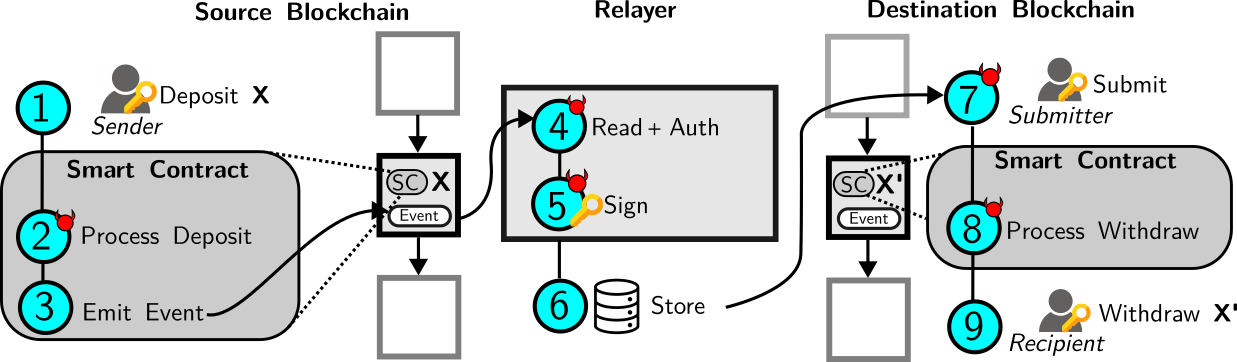
\includegraphics[width=0.8\textwidth]{fig/bridge_arch.pdf}
%%command for cropping pdf
%%gs -sDevice=pdfwrite -o bridge_arch_crop.pdf bridge_arch.pdf
\caption{Cross-chain token bridging and the different steps attackers can exploit to withdraw unbacked deposits.}
\label{fig:cross-chain}
\end{figure*}

\section{Background}
\label{sec:background}
% In this section, we start by providing an overview of blockchain technology. We then describe how cross-chain bridges work followed by the threat model we consider in this paper.
% In this section
We first give a brief introduction to smart contract blockchains
and cross-chain bridges. We then describe how bridges, under attack, collapse in
practice.

\subsection{Smart-contract Blockchains} Modern DeFi protocols (e.g.,
decentralized exchanges and lending protocols) are built on top
of ``smart-contract'' blockchains, like Ethereum. At their core, these chains, like
the original Bitcoin blockchain, are distributed ledgers that manage accounts
(public keys) and their balances (in native tokens like Ethereum's ETH). Users
interact with these chains by signing and broadcasting (to the distributed nodes
that make up the chain network) transactions that, for example, transfer
funds from their account (using the corresponding account private key) to
another user's account.

Ethereum, and the smart-contract chains it inspired since its release in 2015,
differ from Bitcoin by extending the ``simple'' distributed ledger with a smart
contract execution layer. A smart contract on Ethereum is an \emph{internal}
account---and, like a normal, \emph{externally owned} account (EOA), it has a
balance---that has associated \emph{code} (EVM bytecode), which implements the
smart contract's program logic, and \emph{storage}, which persists the program's
state across executions. Users interact with (i.e., execute) smart contracts
much like they do when transferring funds from their account: they sign a
transaction that encodes the smart contract to call (i.e., the contract address),
the particular function to execute, and the arguments to call the function with.
Instead of simply transferring funds from the user's account, then, executing
such a \emph{smart-contract call} transaction amounts to executing the smart
contract bytecode---and any smart contracts the contract itself calls.
    
% \begin{lstlisting}
% contract USDC{
%   mapping(account => amount) _balances;
%   event Transfer(from, to, value);
%   function transfer(to, amount) {
%     address from = msg.sender; // user
%     // ... validate user has enough balance
%     _balances[from] -= amount;
%     _balances[to] += amount;
%     emit Transfer(from, to, amount);
%   }

%   function mint(to, amount) {
%     _balances[to] += value;
%     emit Transfer(address(0), to, amount);
%   }

%   function burn(from, amount) {
%     // ... validate user has enough balance
%     _balances[from] -= amount;
%     emit Transfer(from, address(0), amount);
%   }

%   function safeTransferFrom(from, to, amount){ 
%     // ... transfer tokens; revert if failed
%   }
% }
% \end{lstlisting}


\begin{figure}[t]
    \centering
    \includegraphics[width=\columnwidth]{fig/usdc-contract-2sp.pdf}
    \caption{Simplified USDC ERC-20 Token Contract.}
    \label{fig:erc20}
\end{figure}


    

% \lstdefinestyle{myStyle}{
%     belowcaptionskip=1\baselineskip,
%     breaklines=true,
%     % frame=none,
%     % numbers=none, 
%     basicstyle=\footnotesize\ttfamily,
%     % keywordstyle=\bfseries\color{green!40!black},
%     % commentstyle=\itshape\color{purple!40!black},
%     % identifierstyle=\color{blue},
%     backgroundcolor=\color{gray!10!white},
%     language=Python,
% }

% \lstdefinestyle{customc}{
%   belowcaptionskip=1\baselineskip,
%   breaklines=true,
%   frame=L,
%   xleftmargin=\parindent,
%   language=Python,
%   showstringspaces=false,
%   basicstyle=\footnotesize\ttfamily,
%   keywordstyle=\bfseries\color{green!40!black},
%   commentstyle=\itshape\color{purple!40!black},
%   identifierstyle=\color{blue},
%   stringstyle=\color{orange},
% }


\subsection{ERC-20 Tokens}
One of the immediate applications of smart contracts---and to date still one of
most popular---is to create custom tokens (or coins).  To launch a new token, an
organization no longer needs to launch a new blockchain; they can instead deploy
a new contract that implements the ERC-20 token standard interface on a chain
like Ethereum and take advantage of existing on-chain infrastructure like
decentralized exchanges that make it easy to, for example, trade one kind of
token for another---both native tokens (e.g., ETH) and other tokens.\footnote{
    Most EVM chains, i.e., chains that use Ethereum's execution layer,
    follow Ethereum standards like ERC-20. Most non-EVM chains like Solana
    (which have different execution models) have similar standards (e.g., SPL
    tokens in Solana's case).
}

Figure~\ref{fig:erc20} shows a simplified variant of one such token
contract---the USDC \emph{stablecoin} contract.  This contract tracks
how many USDC tokens an account has and governs the spending of these
tokens (much like a bank governs bank notes).  For example, the
contract's \texttt{mint} function lets Circle (the company that owns
the USDC contract) mint new tokens into a user's account---e.g., after
receiving the corresponding payment from the user off-chain (in US
dollars, as USDC tokens are pegged to the US dollar).  The contract
exposes the ERC-20 interface that lets users (and smart contracts)
transfer tokens from their account by simply calling functions like
\texttt{safeTransferFrom}, and, in turn, use the tokens in any DeFi
protocol (e.g., lending the USDC to different markets, exchanging USDC
for ETH,
% buying NFTs using the USDC,
etc.). Finally, the contract's
\texttt{burn} function ``burns'' a token out of circulation---and
emits an event (Figure~\ref{fig:erc20-event}) that Circle's off-chain code looks for before allowing
a user to withdraw the corresponding USD fiat off-chain.

% \subsection{Blockchain Basics}
% In this section, we cover the basic concepts of blockchain technology, including blockchains, smart contracts, transactions, accounts, and tokens.

% \textbf{Blockchains.} A blockchain is a distributed ledger that stores data (e.g., account balance) in a transparent and tamper-proof manner. It consists of a chain of blocks, where each block contains a certain amount of data, a reference to the previous block (thus forming a chain), and other information such as timestamp. Blockchains are maintained by a network of nodes that validate data in the blocks and reach consensus on the state of the ledger.\alex{somehow have to mention Solana and Ethereum and others?}
% % It consists of a series of blocks that are linked together via cryptography (thus forming a chain) [65]. These blocks are immutable and can be used to store data (e.g., transactions). They are also maintained by a distributed network of nodes, removing the need of a central server. 

% \textbf{Smart Contracts.} Smart contracts are programs that can be executed. Typically, smart contracts are first written in high-level programming languages such as Solidity or Rust. Then, they are compiled into bytecode and deployed to the blockchain. Upon deployment, each smart contract is assigned a unique address and becomes immutable. After deployment, they can be executed based on the input provided and the logic programmed into the contract.

% % , compiled into bytecode, and deployed to the blockchain. The input and execution of smart contracts are all recorded on the blockchain. They 

% % are stored and executed on blockchains. They are used to encode business logic, enforce rules, and automate processes. Smart contracts are written in high-level programming languages, compiled into bytecode, and deployed to the blockchain. Once deployed, smart contracts are immutable and can be interacted with by sending transactions.

% % self-executing programs that run on blockchains. They are used to encode business logic, enforce rules, and automate processes. Smart contracts are written in high-level programming languages, compiled into bytecode, and deployed to the blockchain. Once deployed, smart contracts are immutable and can be interacted with by sending transactions.

% \textbf{External Owned Accounts.}  Externally owned accounts (EOAs) represent users and are controlled by private keys. Users can interact with other users or deployed smart contracts by initiating a transaction from their EOAs. To initiate a transaction, a user specifies the recipient (the address of an EOA or a smart contract), the amount of assets to transfer, and any additional input parameters required by the smart contract. 

% % are entities that can send and receive transactions on the blockchain. There are two types of accounts: externally owned accounts (EOAs) and contract accounts. EOAs are controlled by private keys and represent human users, while contract accounts are controlled by smart contracts and represent autonomous entities.

% % Accounts are entities that can send and receive transactions on the blockchain. There are two types of accounts: externally owned accounts (EOAs) and contract accounts. EOAs are controlled by private keys and represent human users, while contract accounts are controlled by smart contracts and represent autonomous entities.


% \textbf{Transactions.} A transaction is a instruction set constructed and signed by a user using their EOA. It typically includes several fields, such as the sender (the EOA that signs the transaction), the recipient (which can be an EOA or a smart contract), the amount of assets to transfer, and the input parameters required by a smart contract. Once signed, the transaction is broadcasted to the network and executed. After successful execution, the resulting state changes are recorded on the blockchain along with the transaction itself.


% \textbf{Tokens.} Every blockchain system has its own native token. For example, Ethereum has Ether (ETH), while Solana has Sol (SOL). In addition to native tokens, blockchains can also host other types of tokens. An example is ERC-20 tokens on Ethereum, which are smart contracts that follow a set of rules and standards. Of particular note, when a user transfers ERC-20 tokens, the ERC-20 token contract emits an event (a type of debug information recorded on the blockchain) that logs certain information. Figure 1 shows an example. The name of the event is Transfer, and the token contract that emits the Transfer event is tagged as USDC. The sender and recipient are represented by their addresses (0x68... and 0xF5..., respectively). The amount of tokens transferred is 212295874.

% \alex{maybe liquidity pool}


\subsection{Cross-Chain Token Bridges}
While smart contracts make it easy to launch new tokens without spinning up new
chains, there is no real shortage of new blockchains being deployed (almost weekly).  Indeed,
the modern blockchain ecosystem is a many-chain ecosystem.  Blockchains like
Avalanche, Base, and Solana have different design points---from cheaper ``gas''
execution costs, to higher throughput, lower latency, and different permission
models---that make them better suited for different classes of application.
This situation has resulted in applications that span many chains and cross-chain
infrastructure that ultimately (try to) allow users to, for example, buy
Dogwifhat NFTs on Solana using USDC tokens on Ethereum.

Core to these applications and infrastructure---and the focus of our work---is
the \emph{cross-chain token bridge}.  At a high level, a cross-chain token
bridge makes it possible for a user to ``transfer'' their tokens from one chain
(e.g., their USDC on Ethereum) to another chain (e.g., Solana) and then use the
transferred tokens on the destination chain (e.g., on a Solana exchange trading
USDC and Dogwifhat).\footnote{While some cross-chain bridges \emph{do} let users
transfer one kind of token (e.g., USDC on Ethereum) for a completely different
kind of token on the destination chain (e.g., Dogwifhat on Solana), these bridges
essentially fuse the cross-chain token bridge with an exchange (or swap). We
focus on token bridges not only because they are fundamental to other kinds of
bridges, but also because they have higher volume, more liquidity, and more
attacks.} Since smart contracts cannot make network requests or otherwise
access sate outside their own storage, a cross-chain token bridge consists of
smart contracts on both the source and destination chains, and off-chain
infrastructure that serves to relay the ``transfer'' call across the two
contracts.

\begin{figure}[t]
\centering
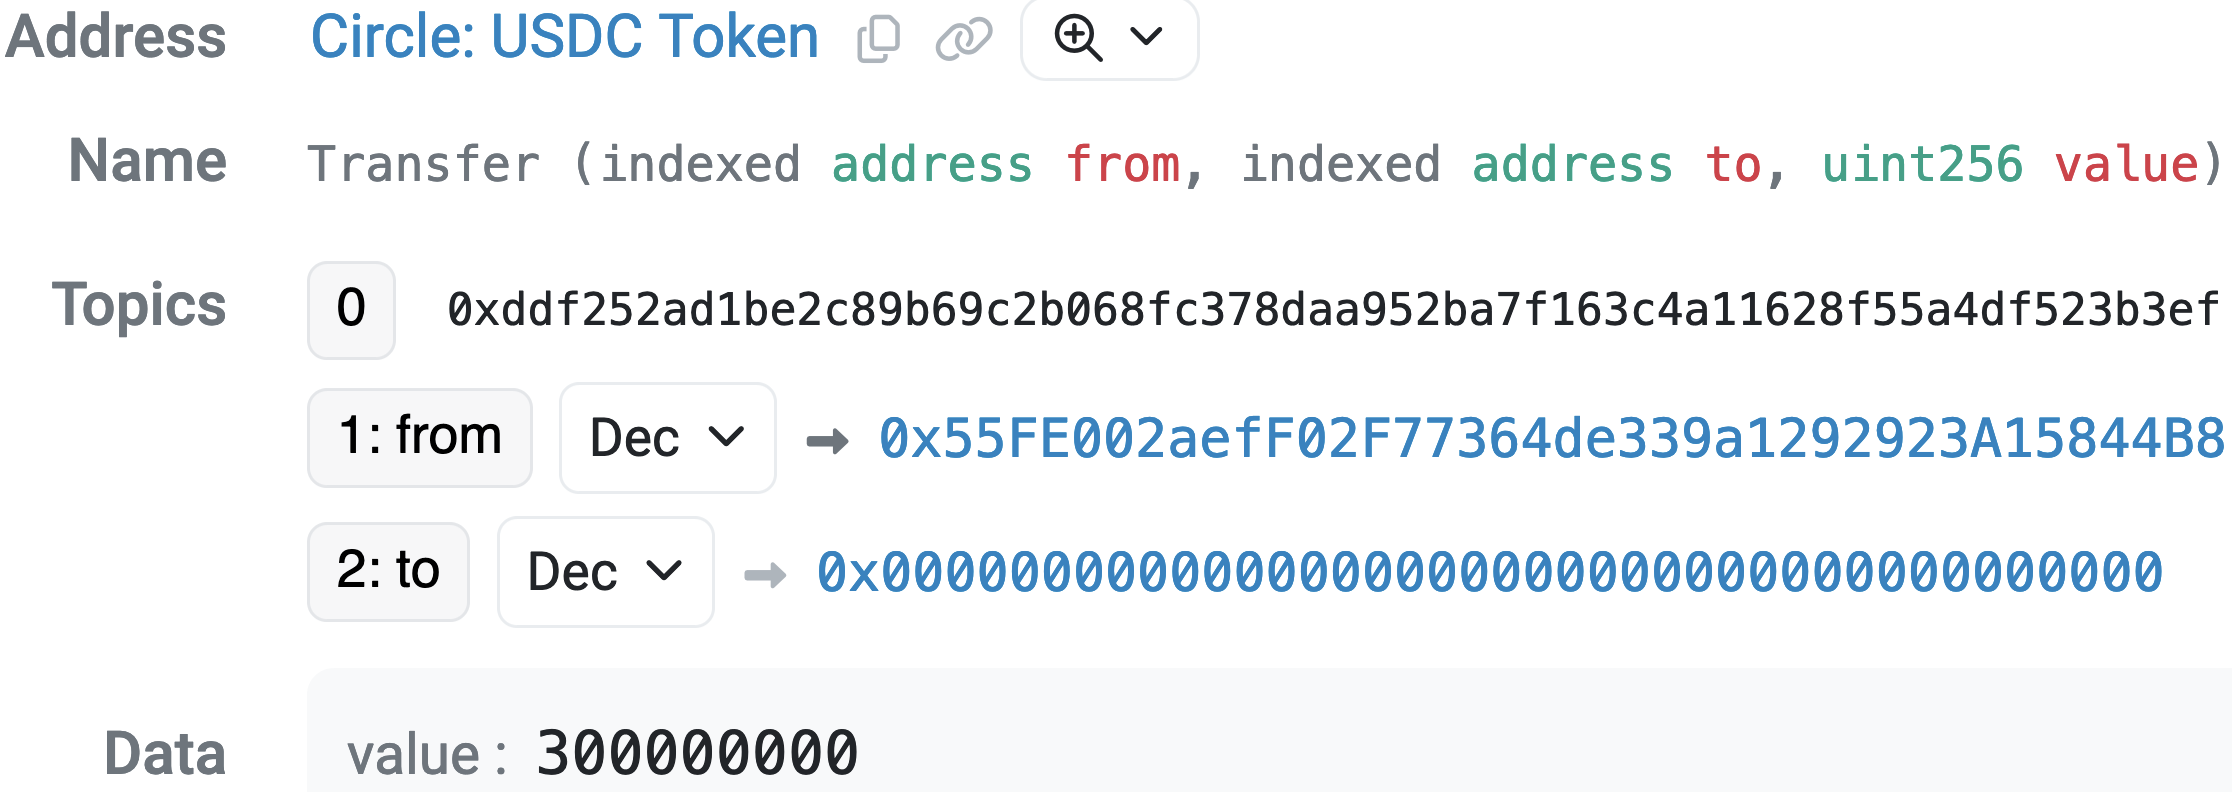
\includegraphics[width=\columnwidth]{fig/token.png}
\caption{Event Emitted by an ERC-20 Token (USDC).}
\label{fig:erc20-event}
\end{figure}

As Figure~\ref{fig:cross-chain} shows, a typical cross-chain token transfer,
i.e., a bridge transaction, consists three phases:

\textbf{1. Deposit (on source chain).}
To initiate a cross-chain token transfer, the user first calls the bridge's
contract on the source chain:
\begin{lstlisting}
deposit(address token, uint256 val, address to) {
  address from = msg.sender;  // user
  address to = address(this); // bridge contract
  // ... validate the ERC-20 token contract
  token.safeTransferFrom(from, to, val);
  emit Deposited(id++, token, from, to, val);
}
\end{lstlisting}
This contract function---a simplified version of the Qubit bridge deposit
function---processes the user's deposit (step 2) by validating the transfer request,
e.g., against a list supported tokens, and then transferring the user's ERC-20
tokens to the bridge contract---recall contracts are accounts with balances.
Then, the function emits an event (step 3) recording the user's deposit details
(including the deposit ID, the ERC-20 token contract address, the recipient on
the destination chain, and value).

\textbf{2. Off-chain relay.}
The emitted event is observed by an off-chain relayer in (step 4),
which constantly monitors the source blockchain.  The relayer first
verifies the authenticity of the deposit event.  If the event is
authentic, the relayer then produces a signed \emph{receipt}
endorsing the deposit (step 5) and, typically, stores the receipt off-chain (step
6).  Finally, this signed receipt is sent to the bridge's withdrawal contract
on the destination blockchain (step 7). Who submits the receipt varies across
bridges---some bridges submit the receipt on the user's behalf (in these cases, the
signed receipt is simply a signed contract-call transaction), while others give
users (and anyone willing to pay gas) the signed receipt and they, in turn,
submit the receipt to the withdrawal contract to complete the transfer. 

\textbf{3. Withdraw (on destination chain).}
The withdrawal contract on the destination chain first processes the withdraw
request by verifying the receipt and transferring the tokens to the recipient
(step 8). In (the simplified) Chainswap's withdraw case, for example, users call:
\begin{lstlisting}
withdraw(uint256 id, address token, address to, uint256 val, Signature[] sigs) {
  _chargeFee();
  // verify receipt
  require(received[id][to] == 0, 'withdrawn');
  for(uint i=0; i < sigs.length; i++) {
    verify_receipt(sigs[i], id, token, to, val);
  }
  received[id][to] = val; // mark as withdrawn
  token.safeTransferFrom(address(this), to, val);
  emit Withdraw(id, token, to, val);
}
\end{lstlisting}
This contract function first charges the caller a fee, then verifies the
deposit details against receipt---both that the deposit was not already
withdrawn and that the receipt signatures are valid---and finally transfers the
tokens to the intended recipient.  We consider a cross-chain transaction
complete when the asset is released to the recipient (step~9).

We expect every cross-chain bridge transaction to uphold the balance invariant:
the value (and kind) of the tokens withdrawn---the outflow---should equal the
value (and kind) of the tokens deposited---the inflow---minus the charged fees.
In practice, they do not.



% \subsection{Cross-Chain Bridges}
% In this section, we begin by providing an example of how a typical cross-chain transaction works. We then discuss the different variants of cross-chain bridges. 
% \subsubsection{A Typical Cross-Chain Transaction}
% Figure~\ref{fig:cross-chain} depicts a typical cross-chain transaction. Starting with the source blockchain, the sender (represented by their EOA) initiates a transaction to transfer assets to the bridge's deposit contract (step 1). The bridge contract then verifies that it has received the assets (step 2). Upon verification, the bridge contract emits an event to record the transfer (step 3). This event is observed by the relaying component (step 4), which typically resides outside and constantly monitors the source blockchain. The relaying component then verifies the authenticity of the event (step 5). If the event is authentic, the relaying component signs the message and stores the signature in a queryable database (step 6). A submitter on the destination blockchain then fetches the signed message from the database (step 7) and sends it to the bridge's withdrawal contract on the destination blockchain (step 8). The bridge contract then verifies the signature (step 9) and transfers the assets to the recipient (step 10). A cross-chain transaction is considered complete when the asset is released to the recipient (step 11).

% % Important things we need in this figure:
%     % source and dst amount
%     % how different vulnerabilities manifest
%         % source
%             % transfer in
%             % verify * emit
%         % relaying component
%             % observe
%             % signs
%         % dst
%             % retrieve & send
%             % verify
%             % transfer out
%     % Players
%         % Sender (in source)
%         % Relayer (in dst)
%         % Receiver (in dst)
    
    



% \subsubsection{Variants of Bridge Implementation}
% Beyond the typical cross-chain transaction described above, there are different ways to implement a cross-chain bridge. We discuss the following variants:

% \textbf{Asset Management.} There are two common ways funds can be released in step 10. The first model is the liquidity pool, which is commonly used when an asset already exists on both blockchains (e.g., USDC already exists on Ethereum and Polygon). Bridges start by creating liquidity pools, to which users can deposit assets and earn fees. When a withdrawal request is made, the bridge releases the funds from the liquidity pool as long as there is sufficient capital in the pool. The second model is mint-and-burn, which can be used regardless of whether the asset exists on the destination blockchain. In this model, the bridge contract mints new tokens on the destination blockchain, which act as representations of the assets on the source blockchain. When a withdrawal request is made, the bridge simply mints new tokens and sends them to the recipient. The recipient can then burn the tokens to receive the original assets on the source blockchain.



% \textbf{Submitter Privilege.} In the flow depicted in Figure~\ref{fig:cross-chain}, once the relaying component has signed the transaction, anyone can fetch the signed message and submit it to the destination blockchain. However, in practice, there is a variant where only privileged EOAs can act as submitters. In this variant, the authenticity of the message is verified by the presence of a privileged key. If bridges choose to operate in this way, they 
% typically simplify step 6 by directly storing the message without signing it.

% \textbf{Transaction Relay.} In the flow depicted in Figure~\ref{fig:cross-chain}, each transaction is relayed individually. In practice, transactions can also be relayed in batches or grouped into a Merkle tree. This approach can improve efficiency. However, while using a Merkle tree is more efficient, it also introduces additional complexity in step 9, where the bridge contract has to verify that a transaction is included in a Merkle tree.

% \textbf{Message Verification Mechanisms.} There are four different mechanisms to verify the authenticity of a message. Namely, external verification, optimistic verification, native verification, and local verification. The details of these mechanisms are not critical for this paper. We provide a brief overview of each model and refer the reader to \alex{cite} for more details. At a high level, external verification indicates that the relaying component resides outside both the source and destination blockchains. The legitimacy of a cross-chain transaction is attested by a third party (or a set of third parties). Native verification, on the other hand, indicates that the relaying component resides within the destination blockchain. In this model, the relaying component typically operates as a light client of the source blockchain and maintains enough information to verify the authenticity of a message from the source blockchain. Optimistic verification improves the efficiency of external verification by assuming that the majority of relayed transactions on the destination blockchain are valid. Instead of attesting to the validity of every transaction, optimistic verification only intervenes when a fraudulent transaction is detected. Finally, local verification means that the two parties involved in a cross-chain transaction (e.g., the sender and the submitter) must cooperate and collaborate for the transaction to succeed.

% \textbf{Token Swap Bridges.} In the above example, tokens released on the destination blockchain are backed by an equivalent amount of assets (less fee) on the source blockchain. However, in practice, bridges can also support token swap. In this case, an asset on the source blockchain is swapped for a different asset on the destination blockchain. For example, a user can swap 1 ETH for 100 USDC. The conversion rate is typically determined by the relaying component and may not be publicly disclosed. 

% \subsubsection{Variants of Verification Mechanism.}
% \textbf{External Verification.} In the most common case, the verification components resides outside both the source and destination blockchains. This is known as an externally verified bridge. The legitimacy and correctness of a cross-chain transaction is determined by a third-party (or a set of third-parties). Common ways to implement external verification include Multi-party Computation and Threshold Signature Scheme.\alex{cite}

% \textbf{Optimistic Verification.} Optimistic Verification improves on the efficiency of external verification by assuming that the majority of transactions are valid. Instead of attesting to the validity of every transaction, optimistic verification only intervenes when a dispute arises. This is known as an optimistic bridge. Concretely, every message that is passed to the destination blockchain is considered "pending" until the dispute window expires. The system relies on one or more honest watchers to dispute the message if it is incorrect. If no dispute arises, the message is considered valid.

% \textbf{Native Verification}
% Contrary to external verification, where the verification component resides outside the source and destination blockchains, the verification component in a natively verified bridge resides within the destination blockchain. Commonly, this is achieved by implementing a light client of the source blockchain within the destination blockchain, which maintains enough information for verifying the authenticity of a message. The security is guaranteed by the validators of the source chain. 


% \textbf{Local Verification}
% \alex{add citation. this is the most confusing one.}
% The basic idea is that the sender and the submitter
% have to cooperate and collaborate for a cross-chain transaction to succeed. 

\subsection{How Bridges Collapse}
In practice, attackers exploited bugs in all three components---the deposit
contract, the relayer, and the withdraw contract---and stole signing keys
to siphon hundreds of thousands of dollars.
%
Figure~\ref{fig:cross-chain} highlights the precise steps in the cross-chain
token transfer that attackers have historically exploited, including:
\begin{CompactItemize}
\item \textbf{Bugs in the deposit contract.} In step 2, the bridge contract
verifies that it has received the correct amount of assets before emitting an
event. Bugs in this verification logic could allow an attacker to deposit a
smaller amount of assets than what is recorded by the bridge in the event (step
3). For example, Qubit's \texttt{deposit} function  (see above) did not properly validate the token address. This bug allowed an attacker to pass \texttt{0} for the token address, so the contract function did not actually transfer any funds from the attacker's account but still emitted a \texttt{Deposit} event which allowed the attacker to withdraw actual tokens on the destination chain~\cite{qubit:rekt}.

\item \textbf{Bugs in the off-chain deposit verification.} In step 5, the
relayer verifies the authenticity of the deposit event emitted by the
bridge contract, including whether the event is emitted by the bridge's
designated contract.  Bridges that do not correctly verify
deposits would allow attackers to withdraw assets that are never deposited.
% ---and this 

\item \textbf{Stolen relayer (or submitter) keys.} In step 5, the relayer signs the deposit receipts which are then submitted to the withdrawal
contract as evidence of a valid deposit. If the relayer key is compromised
(e.g., as with the Ronin bridge~\cite{roninattack}) the attacker can forge a
valid receipt and then withdraw assets that were never deposited by calling
\texttt{withdraw} with the forged receipt.

The same is true for bridges that submit receipts on behalf of users---and
essentially restrict the \texttt{withdraw} callers to privileged submitter
accounts. The bridge submitter keys (step 8) have similarly been compromised
(e.g., as with AnySwap~\cite{anyswapattack}) and used to withdraw
unbacked deposits.

\item \textbf{Bugs in the withdraw verification.} In step 8, the bridge contract
verifies that the messages are signed by the relayer and have not
been replayed. Bugs in this verification logic (e.g., as we saw with
Wormhole~\cite{wormholeattack}) have allowed attackers to supply ``valid''
payloads that were not signed by the relayer and replay withdrawal
requests with valid deposit receipts that have already been withdrawn.
\end{CompactItemize}


% Liquidity Pool vs Mint-and-Burn. Example USDC on ETH and Polygon
% Verification Modes
% \subsection{Threat Model}
% In this section, we describe the attack surfaces that are in scope for this paper. Importantly, we assume that deposits and withdrawals are made through designated functions and that funds cannot be withdrawn through functions other than the designated withdrawal function(s). Given this setup, we consider the following attack surfaces:

% \textbf{Buggy Deposit Verification.} In step 2, the bridge contract verifies that it has received the correct amount of assets before emitting an event. Bugs in this verification logic could allow an attacker to deposit a smaller amount of assets than what is recorded by the bridge in the event (step 3).

% \textbf{Buggy Event Verification.} In step 5, the relaying component verifies the authenticity of the event emitted by the bridge contract, including whether the event is emitted by the bridge's designated contract. Failure to do so could allow an attacker to withdraw assets that were never deposited.

% \textbf{Compromised Relaying Key.} In step 6, the relaying component signs the message and stores the signature in a queryable database. If the relaying key is compromised, an attacker could forge a message and withdraw assets that were never deposited.

% \textbf{Compromised Submitter Key.} In step 8, some bridges operate in a privileged submitter mode, where the presence of the privileged submitter key is the only requirement to attest to the authenticity of a message. In this case, if the submitter key is compromised, an attacker could submit a forged message and withdraw assets that were never deposited.

%\textbf{Buggy Withdraw Verification.} In step 9, the bridge contract verifies that the messages are signed by the relaying component and have not been replayed. Bugs in this verification logic could allow an attacker to verify payloads that are not signed by the relaying component or to replay a message that has already been processed.

In this paper, we assume an attacker can exploit any of the aforementioned
components or otherwise control the relayer (or submitter) keys.
In the next section, we show that this attacker model and our simple
\emph{balance invariant checking} captures the largest attacks on cross-chain
bridges that have happened in the past.  In Sections~\ref{sec:live-audit} we show
that monitoring withdrawals and deposits on the source and destination chains
can be used to detect similar attacks in the future.  Finally, in
Section~\ref{sec:active-protect} we describe an \emph{announce-then-execute} bridge
design that enforces this invariant to prevent attacks before they happen.

We note that while our threat model captures a wide variety of vulnerabilities,
it is not exhaustive.  As with any detection system, an attack that violates one
of our assumptions (e.g., avoids violating the balance invariant by transferring
funds off-bridge or not having a withdrawal, subverts the transaction data used to validate the invariant,
etc.) might succeed.  
We similarly consider other smart contract bugs (beyond bugs in deposit and withdrawal functions) and account key compromises out of scope---and instead focus
on the cross-chain bridging aspects which are relatively less well understood.
As we show later, our model captures the largest attacks on
cross-chain bridges that have happened in the past and systems can use
it to prevent similar attacks in the future.


%% While our approach captures a variety of vulnerabilities, it is by no
%% means exhaustive. For example, a key assumption we make is that
%% withdrawal are done through designated withdraw functions. However, if
%% an adversary is able to compromise the key to account that holds the
%% funds for the bridge, they could simply transfer the funds to another
%% account and then withdraw them without going through the designated
%% withdraw function(s). Similarly, if an adversary is able to withdraw
%% funds by repurposing other functions (e.g., the deposit function), our
%% approach would not detect it. Moreover, if an attack transaction does
%% not involve a withdrawal, our approach would not detect it. Last but
%% not least, if an attack is somehow able to profit without breaking the
%% balance invariant, our approach would not detect it.  However, we
%% believe that our approach is a important first step in using
%% accounting principles to protect bridges from theft and that it can be
%% extended to address these and other vulnerabilities in the future.

\section{Approach}
\label{sec:meth}

The core hypothesis of our work is that value should be conserved
within cross-chain transactions.  That is, that the value of the asset
inflow in such a transaction (i.e., the deposit) should equal the
value of the asset outflow (i.e., the withdrawal).  In token transfer
bridges, this invariant corresponds to a balancing of the inflow
tokens and the outflow tokens (less any fees or transaction costs
incurred by the bridge itself).  When this balance invariant does not
hold it allows a range of opportunities for fraud, all of which
involve greater outflows (withdrawals) than inflow
(deposits). Figure~\ref{fig:invariant} illustrates such an outcome by 
graphing the \emph{aggregate} difference between bridge inflow (on
Ethereum) and outflow (on Solana) leading up to and during the
February 2022 attack on the Wormhole bridge.  The net difference is
consistently near zero, with only short positive deviations
(representing delayed withdrawals) until the attack in January, at
which point there are significant withdrawals without matching
deposits---producing a large negative difference.

Testing this invariant on a \emph{per transaction basis} is
straightforward in principle. However, since bridge transaction formats are
not standardized, it requires a range of per-bridge and per-chain
parsing in practice.  Our methodology for normalizing this information
focuses on two key pieces of information: a) identifying each bridge
transaction---a composite of a deposit (inflow) transaction on a
source blockchain and a withdrawal (outflow) transaction on
another---and b) identifying the value transferred in each such bridge
transaction.

\begin{figure}[t]
  \centering
  \includegraphics[width=0.7\columnwidth]{fig/sec25_plot_wormhole.pdf}
  \caption{Total Inflow (on Ethereum) - Total Outflow (on Solana) Over Time: Wormhole Attack in Feb 2022.}
  \label{fig:invariant}

\end{figure}


\subsection{Identifying Bridge Transactions}
For almost all bridges, identifying their component (per-chain) inflow
and outflow transactions is straightforward --- bridges typically use
explicit events on each chain to signal if a given transaction is a
deposit or withdrawal.\footnote{One key exception to this rule is the
  Wormhole bridge which, until late 2023, did not emit specific
  events when executing a withdrawal transaction.  In this case, we infer that a withdrawal took
  place by looking for transactions that invoke functions designated for performing withdrawal operations (e.g., \textit{completeTransfer}).
  %have synthesized such an event ourselves by parsing the function
  % names called by the transaction to .  
  It also appears to be widely understood today that emitting
  explicit events is a best practice.}

Pairing these component transactions (i.e., matching deposits on one
chain to withdrawals on other) can be performed in several different
ways.  The easiest, and most common, is via a unique transaction
identifier. Such IDs are typically generated by the bridge on the
\emph{source chain} during a deposit transaction and then copied into
the withdrawal transaction on the destination chain.\footnote{These
  unique IDs are commonly simple global variables incremented with
  each new transaction.}  However, instead of an explicit ID, some
bridges use a hash of the deposit transaction for the same purpose
(e.g., for Anyswap, each withdraw transaction will include the hash of
its corresponding deposit transaction).\footnote{We note that to prevent potential replay attacks, bridge implementers should also include an ID that uniquely identifies individual deposit events within a transactions. Sadly, this is often not the case.}  Finally, in a handful of cases there are
no ``inband'' identifiers that can be used to associate transactions.
We believe this is a poor design choice that is fundamentally in
conflict with auditability.  However, even in these cases, for the
purpose of our analysis we have been able to pair transactions using
explicit query APIs provided by the affected bridges
services.\footnote{For example, when a bridge transaction on the Poly
  Network bridge includes a withdrawal from Curve (a kind of liquidity
  pool) or when a bridge transaction on the Binance Token Hub includes
  a Binance Smart Chain (BSC) withdrawal, it is not possible to
  identify the partner deposit from blockchain data alone and we must
  make use of ``out of band'' data available through their respective
  bridge query APIs.}

  At the end of this process, we identify a comprehensive collection
  of ``bridge transactions'' (a pair of transactions from two
  different blockchains that were used by the bridge to transfer
  value across them). While the vast majority of bridge transactions
  are pairs of deposit and withdrawal transactions, a handful of
  bridge transactions are either withdrawal-only (e.g., in the case of
  attacks) or deposit-only (e.g., if the user chooses to delay their
  withdrawal).

% And for 
% a handful of bridge transaction, they are either withdrawal-only or deposit-only, and we treat them as singleton transactions.
%  and a handful of singleton
% transactions (i.e., which involve the bridge, based on their
% addresses, but are withdrawal-only or deposit-only).


%For example, with the Binance bridge, the matching transaction for a BSC transaction can only be identified by querying the API. 
%%% here.
%Similarly, for Poly Network bridge, when users withdraw from Curve (a kind of liquidity pool), the matching deposit amount is not recorded on the blockchain, as its a special type of withdrawal where the matching deposit is computed off-chain and only available through the API. In this case, we also rely on Poly Network's API to pair the deposit and withdraw transactions, if the deposit transaction is from Curve. \elisa{It might be nice to give a reason why the pairing info is not available for these cases if we know.} 




%\textbf{Using Unique ID.} Most of the bridges\alex{how many?} will create a unique id for each deposit transaction (incrementing by 1).
%A withdraw transaction will contain this unique id. We can then use this unique id to pair the deposit and withdraw transactions.



%\textbf{Using the transaction hash of the deposit transaction.}
%Another way to pair deposit and withdraw transactions is to use the transaction hash of the deposit transaction. A withdraw transaction will include the transaction hash of the corresponding deposit transaction hash. We can then use this information to pair the deposit and withdraw transactions.

%\textbf{Using the official API.}
%Some bridges provide APIs to query matching deposit and withdraw transactions. While this feature mostly exist for user convenience, sometimes we have to rely on this API to pair deposit and withdraw transactions, as the pairing information is not directly available as part of the withdraw transaction.\alex{maybe we should hedge here and say its not trivial to get the information.} 
%For example, with the Binance bridge, the matching transaction for a BSC transaction can only be identified by querying the API. 
%%% here.
%Similarly, for Poly Network bridge, when users withdraw from Curve (a kind of liquidity pool), the matching deposit amount is not recorded on the blockchain, as its a special type of withdrawal where the matching deposit is computed off-chain and only available through the API. In this case, we also rely on Poly Network's API to pair the deposit and withdraw transactions, if the deposit transaction is from Curve. \elisa{It might be nice to give a reason why the pairing info is not available for these cases if we know.} 

\subsection{Identifying the Value Transferred}
Many bridge transaction event formats explicitly identify the amount
and kind of tokens transferred. However, some bridges do not emit this
information and others can be unreliable.\footnote{For example, as
  mentioned earlier, pre-2024 Wormhole does not emit an event for
  withdrawal transactions. Other examples include the Meter bridge and
  Qubit bridge, which attempted to verify the number of tokens
  received but had exploitable bugs.}  In such cases, we can
frequently make use of the ERC-20 ``Transfer'' event (see
Figure~\ref{fig:erc20-event} for an example) that is emitted when the
contract transfers the tokens from the user's account to the bridge's
account.  This event contains the number of tokens transferred as well
as the sender and recipient addresses, which we use to identify the
number of tokens transferred to or from the bridge.  Because the
Transfer event is adjacent to its associated bridge-generated event,
it is easy to identify and thus establish the number of tokens
transferred.\footnote{As a sanity check, we also require that the
  sender and recipient addresses in the Transfer event are consistent
  with the bridge's defined behavior: for withdrawal transactions, we
  require that the sender is either a mint address (i.e., all-zero
  address) or a bridge-controlled address, while for deposit
  transactions, we require that the recipient is either a burn address
  (i.e., all-zero address) or a bridge-controlled address.}  In a few
implementations, multiple related Transfer events can be emitted at
once, and in these cases we have manually inspected their contracts
and constructed implementation-specific logic to account for this
behavior.  Another special case is caused by so-called ``reflection
tokens'' in which the number of tokens logged in the event (the value
field in Figure~\ref{fig:erc20-event}) is dynamically adjusted based
on a combination of the intended number and the total token supply.
For such cases, we either rely on bridge events which capture the
intended number of tokens transferred or implement token-specific
logic to recompute the value accordingly.  Finally, native tokens have
no Transfer event (since they are not ERC-20 tokens), but thus far we
have either been able to recover the number of tokens transferred from
bridge events or so-called ``internal transactions''.

To summarize, while it is certainly possible to create a bridge
transaction protocol that records insufficient data to match deposits
and withdrawals, or for which the number of tokens transferred might
be ambiguous, our empirical experience analyzing 11 bridges and 21
blockchains is that such reconstruction has always been possible.


%When the amount of tokens transferred logged by the bridge is unavailable or unreliable, we can use the Transfer event emitted by an ERC20 token contract to identify the amount of tokens transferred. The Transfer event, part of the ERC20 standard, has been used by prior research in other scenarios.\alex{cite} This event contains the amount of tokens transferred as well as the sender and recipient addresses, which we use to identify the amount of tokens transferred to or from the bridge. Concretely, we observe that for any successful bridge transaction, depending on the order of execution, the transfer event either happens right before or after the bridge-generated event. As a result, we can first locate the bridge event and then look for the Transfer event that happens right before or after the bridge event, which contains the amount of tokens transferred. As additional sanity checks, we also require that the sender and recipient addresses in the Transfer event are consistent with the bridge's behavior. Namely, for withdraw transactions, we require that the sender is either a mint address (e.g., all-zero address) or a bridge controlled address. On the other hand, for deposit transactions, we require that the recipient is either a burn address (e.g., all-zero address) or a bridge controlled address.\alex{do we have to explain the intuition?}


%There are two ways to identify the amount of tokens transferred by the bridge: using the amount logged in a 
%bridge-generated event or using the Transfer event emitted by ERC20 tokens. Specifically, some bridges include the amount of tokens sent or received in their events. However, this information is not always reliable, as bridges can have bugs (typically when they don't verify the amount of tokens they actually received), which is the case for [AL: which]. Additionally, some bridges do not emit this information. In such cases, we can use the token transfer event to identify the amount of tokens transferred, which also serves as the ground truth.

%\textbf{Identifying Token Transferred from Transfer Event.} 
%When the amount of tokens transferred logged by the bridge is unavailable or unreliable, we can use the Transfer event emitted by an ERC20 token contract to identify the amount of tokens transferred. The Transfer event, part of the ERC20 standard, has been used by prior research in other scenarios.\alex{cite} This event contains the amount of tokens transferred as well as the sender and recipient addresses, which we use to identify the amount of tokens transferred to or from the bridge. Concretely, we observe that for any successful bridge transaction, depending on the order of execution, the transfer event either happens right before or after the bridge-generated event. As a result, we can first locate the bridge event and then look for the Transfer event that happens right before or after the bridge event, which contains the amount of tokens transferred. As additional sanity checks, we also require that the sender and recipient addresses in the Transfer event are consistent with the bridge's behavior. Namely, for withdraw transactions, we require that the sender is either a mint address (e.g., all-zero address) or a bridge controlled address. On the other hand, for deposit transactions, we require that the recipient is either a burn address (e.g., all-zero address) or a bridge controlled address.\alex{do we have to explain the intuition?}

%\textbf{Additional Considerations.}
%We note a few additional considerations. First, while the transfer action usually results in a single event, there are cases where multiple Transfer events are emitted. In such cases, we need to incorporate token-specific logic to capture a series of Transfer events to identify the amount of tokens transferred. For tokens exhibiting this behavior, we manually examine their code and account for their logic in our analysis.
%Next, for transfers involving native tokens, the value sometimes is included in internal transactions, and no event is emitted. We use the internal transactions to identify the amount of tokens transferred. Lastly, for a special type of tokens called reflection tokens, we need to account for the reflection mechanism. Specifically, reflection tokens have a mechanism where the real amount of tokens transferred is dynamically adjusted based on intended amount and total supply. For some tokens, they emit events that include enough information to recompute the intended amount. We thus use this information to identify the intended amount of tokens transferred. For other tokens, they do not provide such information. However, for those cases, conveniently, the bridge event includes the intended amount of tokens transferred. We thus revert back to use the amount logged by the bridge.\footnote{The delta between the intended amount and the real amount is very small (typically within a factor of 0.01). Thus, even if the initial amount is not logged by the bridge, the intended amount can still be bounded.}

\subsection{Checking the Balance Invariant}
Once we have identified both sides of the bridge transaction and the
number of tokens transferred by the bridge, we can verify if the
balance invariant holds: for each bridge transaction (including those
that are withdrawal-only), does the number of tokens transferred from
the bridge---the withdrawal amount---match the number of tokens
received by the bridge---the deposit amount?

However, a key complication is that bridges can charge fees and, while
these fees can sometimes be paid ``out of band'', it is not uncommon
for them to be subtracted from the tokens received on deposit.  To
account for this behavior (i.e., outflow = inflow - costs), we must be
able to determine such costs on a per-transaction basis.
In most cases, fees can be accounted for in a straightforward manner:
they either are made explicit in bridge-generated events (and can thus
be accounted for directly) or can be calculated based on either
published fee schedules or inferred fee schedules (i.e., since all
transactions are typically subject to the same fixed or percentage
fees).


%In practice there are two (additional) factors that influence this
%calculation. First, tokens could have different decimals on different blockchains.
%We account for this difference by retrieving the token's decimal information on each blockchain
%and normalizing the amount of tokens transferred accordingly. More concretely, token transfer values are expressed in the smallest unit of the token.

%\deian{dont use passive voice---who expresses them?} As an example, for a token with 6 decimals, 1 token = $10^6$ units. For the amount $212295874$ in Figure~\ref{fig:erc20-event}, if the token has 6 decimals,
%the normalized amount of tokens (also known as the whole unit amount) transferred to $212295874 / 10^6 = 212.295874$. 
% this by... XXX alex... I don't understand the sentence ``by using
% the token's decimal information to normalize the amount of tokens
% transferred''.

%.  In others, they may not be reported, but
% can be calculated based on either published fee schedules or inferred
% fee schedules (i.e., since all transactions are typically subject to
% the same fixed and percentage fees).

In some cases, the precise value of fees may be difficult to determine
retrospectively because they depend on some external contemporaneous
value not recorded in the transaction (e.g., fees valued in US dollars
implicitly depend on the exchange rate of a given token at that time).
While such ambiguity could be further minimized with additional data,
in our work we manage this issue by defaulting to a simple rule
that the number of tokens withdrawn should not exceed the number
deposited.






%We note a few additional considerations here. First, we note that the amount typically includes decimals, and the same token can have different number of decimals on different blockchains. We account for this by using the token's decimal information to normalize the amount of tokens transferred. Next, for some bridges, the amount of tokens transferred is not equal to the amount of tokens received because of the bridge fee. We address this issue by using the fee information provided by the bridge. When the fee information is unclear or specified in real currency (e.g., US dollars), we simply require that the amount of tokens transferred is less than or equal to the amount of tokens received by the bridge. 



\begin{facingcaption}{table}
\caption[The Blockchains \offlinetool Supports and the Cross-chain Bridges that Operate on Them.]{The blockchains \offlinetool supports and the cross\-chain bridges that operate on them.  While a particular attack on a
    bridge involves two chains, I collect deposit and withdrawal
    transactions for a bridge on all chains that the bridge supports. Anyswap is also known as Multichain.}
\label{table:chain_bridge_full}
\renewcommand\tabularxcolumn[1]{>{\RaggedLeft\arraybackslash}p{#1}}
\parindent=0pt
\setbox0=\vbox{%
\vsize\textwidth
\hsize\textheight
\linewidth\hsize
\columnwidth\hsize
\textwidth\hsize
\textheight\vsize

\begin{tabular}{ll}
  \toprule
  \textbf{Blockchain} & \textbf{Bridges that Operate on the Chain} \\
  \midrule
  Arbitrum &      Anyswap, Poly Network, Wormhole \\
  Avalanche &     Anyswap, Poly Network, Meter, Nomad, Wormhole \\
  % Base &  \\ \hline
  Binance Beacon & Binance Token Hub \\
  Binance Smart  & Anyswap, Binance Token Hub, Chainswap, Harmony, Meter, Omni, Poly Network, Qubit, Wormhole \\
  Celo &          Anyswap, Poly Network, Wormhole \\
  ETH &           Anyswap, Chainswap, Harmony, HECO, Meter, Nomad, Omni, Poly Network, Qubit, Ronin, Wormhole \\
  % ETHPoW &  \\ \hline
  EVMOS &         Anyswap, Nomad, Omni \\
  Fantom &        Anyswap, Poly Network, Wormhole\\
  Gnosis &        Omni, Poly Network       \\
  Harmony &       Anyswap, Harmony Bridge, Poly Network \\
  HECO &          Anyswap, Chainswap, HECO, Poly Network \\
  Meter &         Meter\\
  Metis &         Anyswap, Poly Network\\
  Milkomeda &     Nomad \\
  Moonbeam &      Anyswap, Meter, Nomad, Wormhole\\
  Moonriver &     Anyswap, Meter \\
  OKT Chain &     Anyswap, Chainswap, Poly Network \\
  Optimism &      Anyswap, Poly Network, Wormhole\\
  Polygon &       Anyswap, Chainswap, Poly Network, Wormhole \\
  Ronin &         Ronin\\
  Solana &        Wormhole\\
  % Sui &  \\ \hline
  \bottomrule
\end{tabular}


\singlespacing
}
\centerline{\rotatebox{90}{\box0}}
\end{facingcaption}



% \begin{table*}[t]
% \centering
% \begin{tabular}{|p{2.8cm}|c|r|c|c|c|c|}\hline
%     \textbf{Name} & \textbf{Date} & \makecell{\textbf{Amount} \\ (millions)} & \makecell{\textbf{TXNs}\\ \textbf{Analyzed}} & \makecell{\textbf{Reported Malilicious} \\ \textbf{TXNs Flagged}} & \makecell{\textbf{Unreported Malilicious} \\ \textbf{TXNs Flagged}} & \makecell{\textbf{Other TXNs} \\ \textbf{Flagged}} \\ \hline
%     Ronin & 2022-03 & 624.0 & 2.8m & 2/2 & 0 & 0\\ \hline
%     PolyNetwork 2021 & 2021-08 & 611.0 & 292k& 18/18& 0 & 1\\ \hline
%     BNB Bridge & 2022-10 & 587.0 & 1.4m & 2/2 & 0& 0\\ \hline
%     Wormhole & 2022-01 & 360.0 & 500k& 1/1 & 0 & 2\\ \hline
%     Nomad & 2022-08 & 152.0 & 35k& 962/960 & 0& 0\\ \hline
%     Harmony & 2022-06 & 100.0 & 336k& 15/15& 0& 43\\ \hline
%     HECO & 2023-11 & 86.0 & 23k & 8/8 & 0 & 73\\ \hline
%     Qubit & 2022-01 & 80.0 & 260 & 16/16 & 0& 114\\ \hline
%     Anyswap & 2021-07 & 7.9 & 26k & 4/4 & 3 & 2 \\ \hline
%     PolyNetwork 2023 & 2023-06 & 4.4 & 239k & 136/136 & 0 & 28\\ \hline
%     Chainswap (07-12) & 2021-07 & 4.4 & 53k & 1136/?& 0 & 17\\ \hline
%     Meter & 2022-02 & 4.3 & 14k& 5/4 (we have 1 more)& 0& 0\\ \hline
%     % Chainswap (07-02) & 2021-07 & 4.4 & & & & \\ \hline (worth noting. still from bridge's user)
%     % Omni\alex{will be removed} & 2022-09 & 0.5 & & & Many & \\ \hline
% \end{tabular}
% \caption{List of attacks on cross-chain bridges studied, sorted by amount stolen.}
% \label{table:bridges-and-txns-flagged}
% \end{table*}

%% \begin{table*}[h]
%% \centering
%% \begin{tabular}{p{2.8cm}cr@{}l}
%%     Ronin & 2022-03 & 624 & \mil \\
%%     Ronin & 2022-03 & 4 & .4\mil \\
%% \end{tabular}
%% \label{table:bridges-and-txns-flagged2}
%% \end{table*}
\begin{table*}[t]
\scriptsize
\centering
\begin{tabular}{p{2.7cm}rS[table-format=4.2]rrcrrr}
  \toprule
%  \textbf{Name} & \textbf{Date} & \makecell{\textbf{Amount} \\ (millions)} & \makecell{\textbf{TXNs}\\ \textbf{Analyzed}} & \makecell{\textbf{Reported Malilicious} \\ \textbf{TXNs Flagged}} & \makecell{\textbf{Unreported Malilicious} \\ \textbf{TXNs Flagged}} & \makecell{\textbf{Other TXNs} \\ \textbf{Flagged}} \\
  \textbf{Name} & \multicolumn{1}{c}{\textbf{Date}} & {\textbf{Loss (USD)}} & \textbf{Analyzed} & \textbf{Reported} & \textbf{New} & \textbf{Test} & \textbf{Error} & \textbf{Suspicious} \\
  \midrule
    Ronin & Mar 2022 & \num{624.0}M\xspace & 3.0 & 2                 & - &  -  & - & - \\ % 0
    PolyNetwork/2021 & Aug 2021 & \num{611.0}M\xspace & 292\thou & 18    & - &  -  & 1 & - \\ % 1
    BSC Token Hub & Oct 2022 & \num{587.0}M\xspace & 2.0\mil & 2         & - &  -  & - & - \\ % 0
    Wormhole & Jan 2022 & \num{360.0}M\xspace & 642\thou & 1             & - &  -  & 2 & - \\ % 2
    Nomad & Aug 2022 & \num{152.0}M\xspace & 37\thou & $^\dagger$962      & - &  -  & - & - \\ % 0
    Harmony & Jun 2022 & \num{100.0}M\xspace & 336\thou & 15             & - &  -  & - & 43 \\ % 43
    HECO & Nov 2023 & \num{86.0}M\xspace & 23\thou & 8                   & - &  -  & - & 73 \\ % 73
    Qubit & Jan 2022 & \num{80.0}M\xspace & 260 & 16                     & - & 114 & - & - \\ % 114
    Anyswap & Jul 2021 & \num{7.9}M\xspace & 3.4\mil & 4                & 24 &  -  & 806 & 7 \\ % 2
    PolyNetwork/2023 & Jun 2023 & \num{4.4}M\xspace & 290\thou & 136     & - &  -  & 1 & 27 \\ %28
    Chainswap & Jul 2021 & \num{4.4}M\xspace & 53\thou & $^*$1136        & - &  15 & 4 & - \\ % 17
    Meter & Feb 2022 & \num{4.3}M\xspace & 14\thou & $^\dagger$5          & - &  -  & - & - \\ \midrule % 0
    Total  &          & \num{2.6}B\xspace & 10.1\mil & 2,305             & 24 &  129 & 814 & 150 \\
% 43+73+7+27=150
    \bottomrule
    % Chainswap (07-02) & 2021-07 & 4.4 & & & & \\ \hline (worth noting. still from bridge's user)
    % Omni\alex{will be removed} & 2022-09 & 0.5 & & & Many & \\ \hline
\end{tabular}
% 3000+292+2000+647+35+336+23+2300+240+53+14=8940
\caption[List of Top Attacks on Cross-chain Bridges in the Retrospective
  Analysis]{List of top attacks on cross-chain bridges in the retrospective
  analysis, ordered by amount stolen.  \offlinetool analyzed over
  10\mil bridge transactions (20\mil component deposit and withdrawal transactions)
  %\alex{this is pairs of transactions...i.e., the total number is 2x}
  and identified all bridge transactions previously reported as having
  been associated with the attacks (Reported).  It also identified
  bridge transactions that violated the invariant that were a
  previously unidentified attack (New), test transactions (Test),
  transactions reflecting bugs in implementations or use (Error), and
  suspicious transactions that employ manual signing (Suspicious).
  $^\dagger$\offlinetool identified slightly more transactions than
  were reported by the Nomad~\cite{nomad-groundtruth-github:online}
  and Meter~\cite{meter-groundtruth-tencent:online} bridges for their
  attacks (+2 for Nomad, +1 for Meter).
  %% A blog post mentioned 960 transactions involved in the Nomad
  %% attack, while \offlinetool identified 962.
   $^*$The Chainswap attack only has reports of the malicious deposit
  address~\cite{chainswap-groundtruth:online}, which matches the one
  identified by \offlinetool.
  %% and I report the number of violating transactions
  %% matching that address.
  %
  %% $^\diamondsuit$\offlinetool identified one more violating
  %% transaction than mentioned in online posts~\cite{}, perhaps because
  %% it involved Meter's own chain rather than \geoff{...}.
}
\label{table:bridges-and-txns-flagged}
\end{table*}

\section{Retrospective Analysis}
\label{sec:retro-results}

%% \geoff{somewhere we'll define terminology: ``bridge transaction'' $=$
%%   ``deposit transaction'' $+$ ``withdraw transaction''.  and we'll
%%   note that some malicious bridge transactions might not have a
%%   pairing (e.g., no deposit transaction).}

The basic reasoning motivating the balance invariant is simple: that
legitimate bridge transactions should conserve value.  However, this
assumes a particular model for how bridges are used and operated which
may or may not hold in practice.  To validate our hypothesis, I applied
the balance invariant analysis retrospectively across a large set of
past transactions which, while primarily benign, contain the largest
known bridge attacks during our period of study.  Our goal is both to
show that all real attacks are identified (detection), but also that
the invariant does not alert on large numbers of benign transactions
(bridge compatibility).  Later, in Sections~\ref{sec:live-audit}
and~\ref{sec:active-protect}, I will describe systems for live bridge
monitoring as a third party and a new implementation for preventing
unbalanced transactions from being committed.

%In this section I demonstrate the effectiveness of using the balance
%invariant to identify past cross-chain attacks by performing a
%retrospective analysis of known significant cross-chain attacks.
%Later in Sections~\ref{sec:live-audit} and~\ref{sec:active-protect},
%we describe systems for live bridge monitoring as a third party and a
%new implementation for protecting bridges against transactions that
%violate the invariant.

%For our retrospective analysis, I first describe how I selected the
%bridges and blockchains for our study, and how I collect bridge
%transaction data for the blockchains.  I then show that using the
%invariant correctly identifies all bridge transactions that have been
%reported for major attacks on the bridges, discuss the nature of other
%transactions that violate the balance invariant, and overall show that using
%the balance invariant to alert on suspicious bridge transactions is both
%effective and extremely low overhead.

\subsection{Data Set}
\label{sec:retro-data}

%% I start by discussing our bridge selection, followed by the blockchain selection. I end with an overview of the blockchain data collected and analyzed.

To perform a retrospective analysis I need data for which (at
least some) of the ground truth is known.   In this section I
describe how I chose the bridge attacks I study, the blockchains and
smart contracts involved, and how I collected the historical
transaction data.

%\subsubsection{Bridge Selection}
%\paragraph{Bridge Selection.}
\textbf{Attack Selection.}
%
%% To identify attacks that violate the invariant discussed in the
%% previous section,
I compiled a comprehensive list of attacks on cross-chain
bridges that occurred between January 2021 and December 2023.  I used both academic papers surveying cross-chain
bridge attacks~\cite{lee2023sok, zhang2023sok, zhao2023comprehensive} as well
as industry blog posts that collect and characterize attacks over time~\cite{GithubBridgeBugTracker, SlowMistHackedBridges:online,
  REKTDB:online, Web3Great:online, GithubBridgeHacks2:online}. 
As this chapter focuses on end-to-end auditing of bridge transactions, I filter out attacks
involving blockchains lacking smart contracts such
as Bitcoin (e.g., the pNetwork attack in 2021~\cite{pNetworkhack:online}), attacks on swap bridges (e.g., the Thor bridge attacks~\cite{Thorhack1:online,Thorhack2:online}), attacks that do not involve individual bridge transactions (e.g., the evoDefi attack~\cite{evoDefihack:online}),
and attacks that withdraw funds through other means (e.g., direct transfer from a vault that stores assets for a bridge such as the Multichain 2023 attack~\cite{Multichainhack:online}).  Moreover, given the large number of attacks during this period, I focus on
major attacks with claimed losses greater than \$1 million USD and
exclude the remaining (the sum of losses from these excluded attacks are a small fraction of those in our scope).
% where I discuss scope
% I exclude  attacks as well as swap bridges.
%% I then manually categorize each attack, analyzing blog posts that
%% describe the attack and the transactions involved.
%
%% \alex{we should also mention swap bridge out-of-scope likely somewhere
%%   discussing the invariants (something like I ignore them for the
%%   rest of the paper)} \geoff{the ``on smart contract'' requirement
%%   could also be described earlier when discussing scope}
%
This process yielded 12 attacks on 11 distinct bridges.
%, as summarized in Table~\ref{table:bridges-and-txns-flagged}.
I note that this list
includes the top five attacks on cross-chain bridges in history, which
collectively resulted in more than \$2.6 billion USD in claimed losses.

%\subsubsection{Blockchain Selection}
\textbf{Blockchain Selection.}
% The bridges involved in significant attacks 
%
Validating bridge transactions requires access to
transaction data from both the source and destination chains.  I
support every blockchain involved in the bridge transactions
associated with the 12 attacks, either as the source (or claimed
source) or destination chain.  As a result, I support a total of 21
blockchains that together cover a
broad range of designs, including many of the most popular such as 
Ethereum, Binance Smart Chain, and Solana.
% \footnote{Details about some
% deposit transactions on PolyNetwork (deposits that are used for
% liquidity purposes) are only available through PolyNetwork's API.  We
% support querying PolyNetwork's API, but do not list it as a supported
% blockchain.}
%
Table~\ref{table:chain_bridge_full} lists the blockchains and the
bridges in our retrospective study that operate on them.% \alex{cite}

%% I do not support
%% testnets, as any withdrawal transaction on mainnet that is backed by a
%% deposit on testnet should be flagged. \deian{cut testnet sentence, most people have no clue what that is}

%% \footnote{Our list of supported blockchains includes most of the
%% widely-used and well-developed blockchains. While I could explore
%% additional blockchains, the return on effort is diminishing as adding
%% support for each new blockchain is labor-intensive and is unlikely to
%% yield significant new insights.\alex{Geoff, move this paragraph
%%   around}}



%% \geoff{discuss what aspect of collecting the data requires significant
%% effort}\alex{How about a footnote}


% I then augmented the
% list of supported blockchains by including those that are popular
% among multiple bridges, have a large market cap (according to
% CoinMarketCap), and offer good API support. In total, I support 25
% blockchains.  



%\subsubsection{Smart Contract Selection}
\textbf{Smart Contract Selection.}
%
For each bridge, I comprehensively collected the results of all
versions of its bridging smart contracts on every blockchain I
considered.  In particular, I collected deposit and withdrawal
transactions created by every contract the bridge deployed on
every blockchain I support (typically many more blockchains than the
ones involved in a bridge attack) as well as all versions of the smart
contract implementation for the bridge (bridges evolve their
implementations over time, such as in response to an attack).
%
Since the transactions I collected from this set of smart contracts
are much broader than those just involved in the top 12 attacks I
consider, including them further reinforces our findings that the
alerting workload is very small (Section~\ref{sec:retro-analysis}).

%\alex{chainswap}

%% includes not only the smart contracts involved in the attacks, but
%% also other versions of the smart contracts deployed by the bridges.

%% \alex{make it clear that for every
%%   bridge, I audit every contract it has deployed on every blockchain
%%   I support, which is typically much broader than the set of the
%%   blockchains are attacked}

\begin{figure}[t]
  \centering
  \includegraphics[width=\columnwidth]{fig/sec25_plot_lifespan.pdf}
  % \caption{Timeline of bridge attacks and data collection.}
  \caption[The Lifetime of Bridges in Our Study]{The lifetime of the bridges in our retrospective study.
    Lines start with the bridge's first valid transaction and end with the
    last valid transaction in our data, corresponding to the bridge's
    closure or November 2023 if the bridge was still operating at the
    end of our data set.  Diamonds indicate the dates of attack.}
%  First valid transaction, last valid transaction, and the reported attacks on cross-chain bridges (up to Nov '23).}
  \label{fig:bridge-timeline}
\end{figure}


%\subsection{Data Collection}
%\label{sec:data-collect}
\textbf{Data Collection.}
%Since the attacks I consider involve smart contracts, the smart
%contract input and output provide verbose information for
%understanding the nature of individual bridge transactions.
Collecting smart contract transaction data---the verbose record of
what each contract did---across many chains constitutes the most
time-intensive aspect of performing a retrospective analysis.

For each bridge, I collected deposit and withdrawal transactions for
each of the blockchains it operates on (for the 21 chains I
support) using commercial RPC services which charge for queries.  I
primarily used five commercial services,\footnote{% These five RPC services are:
GetBlock, QuickNode, ChainStack, GoldRush, and Ankr.} 
as no single service supports
all of the blockchains and functionality I need.
For each bridge and blockchain combination, by default I
collected all of the historical transactions generated by its smart
contracts from the genesis of its deployment to the end of November
2023 or the end of its life, whichever came first.

The two exceptions to this rule are the Binance bridge, for which I
limited data collection to a year (six months prior to its attack and
six months after) because of the sheer volume of transactions over its
lifetime (30 million transactions) and the Harmony bridge, whose
contract was reused by another bridge (LayerZero) after its attack
(since LayerZero was not attacked itself, I only consider transactions that were directly associated with Harmony).
% \deian{what does repurposed mean?}\alex{reused}
%Since that bridge was not attacked and is outside our scope, I only
%consider transactions that are part of the Harmony bridge.


%
%% In addition, Binance Beacon Chain does not offer an easy to way filter
%% transactions, and thus I focus on deposit and withdraw transactions
%% on Binance Smart Chain.  \geoff{not sure why we're mentioning this
%%   distinction...is this an explanation for why I do not support
%%   Binance Beacon Chain?}
%
%Next, the Harmony bridge had its contract reused by another
%bridge (LayerZero) after its attack.
% \deian{what does repurposed mean?}\alex{reused}
%Since that bridge was not attacked and is outside our scope, I only
%consider transactions that are part of the Harmony bridge.

Figure~\ref{fig:bridge-timeline} illustrates these bridge lifetimes
with each line starting at a given bridge's first transaction and
ending with its last in our data set.  Diamonds indicate the dates of
individual attacks, emphasizing that many of the bridges closed
shortly after their attacks.

\subsection{Analysis}
\label{sec:retro-analysis}

%% In this section we demonstrate the effectiveness of using the
%% invariant to identify cross-chain attacks by performing a
%% retrospective analysis of known significant cross-chain attacks.

We developed a tool called \offlinetool that pairs deposit and
withdrawal transactions from blockchains into bridge transactions, and
applies the balance invariant and consistency checks on them.  Using
the transactions we collected for the 12 attacks across 11 bridges and
21 chains, \offlinetool analyzed over 10\mil bridge transactions (20\mil individual deposit and withdrawal transactions),
identifying more than 2.3\thou bridge transactions associated with the
attacks and 1.1\thou more that violated the balance invariant.

% 624+611+587+360+152+100+86+80+7.9+4.4+4.4+4.3=2621
% 3000+292+2000+642+37+336+23+3400+290+53+14=8940
% 2+18+2+1+962+15+8+16+4+136+1136+5=2305
% 3+114+15+1+2+72+2+27+15+43+1+1+2=298

Table~\ref{table:bridges-and-txns-flagged} summarizes our results.
For each attack, it shows the bridge involved, the date of the attack,
the claimed loss in USD, the number of transactions \offlinetool
analyzed, and the number and kinds of transactions that violated the
balance invariant.
%
Below we discuss these two categories of transactions in more detail.

Looking forward to Sections~\ref{sec:live-audit}
and~\ref{sec:active-protect}, altogether \offlinetool identified 3,423
bridge transactions (0.03\%) that violated the balance invariant out
of more than 10\mil bridge transactions analyzed.  If the invariant is used by a
third-party auditing or protection system, we note that such an alert
workload has a negligible overhead for manual inspection, typically
raising no more than one alert (or one batch of alerts) every few
weeks.

\subsubsection{Reported}

For each of the 12 significant cross-chain attacks,
Section~\ref{sec:retro-data} describes how we gathered the historical
transactions that correspond to the attacks using external sources.
We use these identified transactions as ground truth for evaluating
the ability of \offlinetool to identify attack transactions.  As shown
in Table~\ref{table:bridges-and-txns-flagged}, when processing the
transaction histories of the chains involved, \offlinetool
successfully identified all 2,305 bridge transactions on the source
and destination chains associated with the attacks (including a few extra ones that are missed by the public reports).

Since we designed \offlinetool to specifically identify such attacks,
these results may not be surprising.  However, they are useful for
confirming that the approach of checking a simple, well-defined
invariant works well.  Moreover, the approach works well across a
variety of models, including bridges that specify fees in a fiat
currency, tokens that use a reflection mechanism, etc.


\subsubsection{Other Violating Transactions}

%% \alex{Two questions:
%% * where do we put the comparison with prior work ()? in discussion, we can say the set of problems are broader\\
%% * cases where we are able to not alert depite the invariant being violated? in discussion, reimbursement transactions.\\
%% }

%The more compelling question
Equally compelling
is the extent to which other, non-attack
transactions violate the balance invariants.  If the
attack transactions are dominated by many false positives, then the
approach becomes less effective.
%
As shown in Table~\ref{table:bridges-and-txns-flagged}, \offlinetool
finds significantly fewer (1,117 compared to 2,305) bridge transactions that were
not previously identified as attacks.  Given the nature of these
additional transactions, though, they do not undermine the
effectiveness of the invariant approach.  By violating the invariant
something highly unusual is taking place.  As a result, we argue that
such transactions should be flagged for further scrutiny and perhaps
even blocked from executing (particularly transactions in the New category and the large transactions in
the Suspicious category below).

To ensure that we have not missed benign explanations for a violation,
we manually inspected violating bridge transactions in at least of one
of the following ways: (1) using blockchain explorers to verify that
the funds have been created by the withdrawal (and if so, whether they
have been moved); (2) searching online for any additional information
about the transaction and addresses involved; (3) checking that if
claimed deposit exists; and (4) examining unredeemed
deposits on the source chain that potentially could have been used to
back the withdrawal (e.g., because the smart contract implementation
changed between the deposit and withdrawal).  If we can manually
reconcile a bridge transaction, we consider it benign
% do not consider it an invariant violation
and do not consider it further.

We group the remaining bridge transactions that violate the invariant
into four categories, which we describe below.  For reference, we also
list some of these bridge transactions in
Table~\ref{tab:xaction-hashes} to provide specific
examples with more detail.

\newcommand{\bridgehash}[1]{\texttt{\zz#1\zz}}%In a perfect world, this would be changed to allow linebreaks anywhere in #1
\def\zz#1{%
 \ifx\zz#1\else
   #1\linebreak[1]\expandafter\zz
 \fi}

\begin{table*}[t!]
\centering
\footnotesize
\begin{tabular}{p{1.5cm}p{5.8cm}cp{5.8cm}p{1.5cm}}
\toprule
\textbf{Bridge\todo{format}} & \textbf{(Claimed) Deposit Transaction Hash} & \textbf{\makecell{Chain \&\\Token}} & \textbf{Withdraw Transaction Hash} & \textbf{\makecell{Chain \\\& Token}} \\
\midrule
Wormhole \#1 & \bridgehash{0x8bbb7befd198a5e90297f451fc43a9e90de083289a041c8af94116c785cf496d} &\makecell{Polygon\\0.5\\WSOL}  & \bridgehash{5AiesW9pKrZvCCJM8QPWmqx...dkadV1waPVLWfsnCMVQmyYaciLxEo} &\makecell{SOL\\650\\USDC}\\[0.2in]
% \hline
Wormhole \#2 & \bridgehash{0x55d1e486a8e2102e07fd6270a03f05bbee7b43bf27ebac97b95b98e068f6740e} &\makecell{Polygon\\4.3k\\MATIC}  & \bridgehash{0xbe81895b1c3172fd69b8d4d9bf726edfdc17083876c440f9414ff316999237d7} &\makecell{AVAX\\2.3k\\WMATIC}\\

% \cline{2-5}
%  & \bridgehash{0x542efe5a7f965b927a294bce7f3a30492d0e2ca60da2e2d6cdfaf523a28a2a9c} & \makecell{Polygon\\0.5 SOL}  &\\ 
\hline

Anyswap \#1 & \bridgehash{0x01ba4719c80b6fe911b091a7c05124b64eeece964e09c058ef8f9805daca546b} & N/A &  \bridgehash{0xf015a6b06a13a08d3499ece17504d14a95d6af3e04ae11f291dca22dbbf6c991}  & \makecell{BSC\\$5*10^{-8}$\\USDC}\\[0.2in]
% \cline{2-5}
% \cline{2-5}
Anyswap \#2 & \bridgehash{0x01ba4719c80b6fe911b091a7c05124b64eeece964e09c058ef8f9805daca546b} & N/A &  \bridgehash{0x9e55b7295880dce76aa8af0f3e3f9e36499ae0bdb28088a5924daf29c6132ceb}  & \makecell{BSC\\55k\\USDC} \\[0.2in]

% \cline{2-5}
Anyswap \#3 & \bridgehash{0xe3b0c44298fc1c149afbf4c8996fb92427ae41e4649b934ca495991b7852b855} & N/A &  \bridgehash{0x4f038804d0622d2eab15d21d902a3fdd3bdfb5427bb5fd65b9eb0a41169534be}  & \makecell{Polygon\\100k\\USDC}\\[0.2in]

Anyswap \#4 & \bridgehash{0x0x0000000000000000000000000000000000000000000000000000000000000000} & N/A &  \bridgehash{0x98aa9e94d4fd0a05c27eb13ac2e699e4426c8dd9d57d04c0fa09cf4951eb2f94}  & \makecell{BSC\\650k\\USDC}\\[0.2in]

Anyswap \#5 & \bridgehash{0x0x0000000000000000000000000000000000000000000000000000000000000000} & N/A &  \bridgehash{0xa67ac5dc308142f89409df89dc85e8fab88c575b3adef77fbc8f51858b7bf7cb}  & \makecell{Polygon\\50k\\USDC}\\[0.2in]

Anyswap \#6 & \bridgehash{0x28b233a4dbda8b4dfae7245b8fff434de95f6dbd101e1a9cb22a95ded1315a16} & \makecell{Fantom\\6.4k\\POPS} & \bridgehash{0x76bdcfd5ddfa358bf4181556e3b4f1fdd2d648a246bfab91386bdfbd7b76d01f} & \makecell{Avalanche\\6.4k\\POPS}\\[0.2in]


& \bridgehash{0xf0b5568dfd8a4559d30adc9dfc881875210a3b9dfa680d392b33eb1d2cc86cfa} & \makecell{Fantom\\6.4k\\POPS} & \bridgehash{0xc86297f14f32a33232149025d4e8f8e50985d76ac1b7ccaf181501820c0b1cf7} & \makecell{Avalanche\\6.4k\\(any)POPS}\\[0.2in]


Anyswap \#7 & \bridgehash{0x0x0000000000000000000000000000000000000000000000000000000000000000} & N/A &  \bridgehash{0xde790e8dc59d8bae7ebdf89c4b75267a6e0783219b32aebe83e112aac6c299f5}  & \makecell{Avalanche\\54k\\USDC}\\ 



\hline
HECO \#1 & \bridgehash{0x6f9d2e82aef87fc649198976974c05d4c540dacca5043ffee619cc33f3ba4cf5} & \makecell{ETH\\5m\\USDT} & \bridgehash{0x628e878fb723cf0dd838eb956ce78d23b45b130876a625fd4d283e62ac2289f0}  & \makecell{HECO\\5m\\USDT}\\[0.2in]

& \bridgehash{0x6f9d2e82aef87fc649198976974c05d4c540dacca5043ffee619cc33f3ba4cf5} & \makecell{ETH\\5m\\USDT} & \bridgehash{0x27a1e6a66b6e0fc5fa805f7400dd07397bb92226926868a82afb44154a32128b} & \makecell{HECO\\5m\\USDT}\\


\hline
Harmony \#1 & \bridgehash{0x559bc92656a6956a5ffe9eea6f14a5d5993520e31a1a08551d5171ad8f658886} & \makecell{BSC\\5.3k\\BUSD} & \bridgehash{0xdf3bf1a8227ede87d7905c026c3b6a3504cc81399ebd08e1273e1a9dd2c748a9}  & \makecell{Harmony\\5.3k\\BUSD}\\[0.2in]

& \bridgehash{0x559bc92656a6956a5ffe9eea6f14a5d5993520e31a1a08551d5171ad8f658886} & \makecell{BSC\\5.3k\\BUSD} & \bridgehash{0x304801a2b33585e6867de0c403535588979ce4d2cf41c6922223d3203589c39d} & \makecell{ETH\\$5*10^{-18}$\\BUSD}\\ 

\hline
PolyNet. \#1 & \bridgehash{0x0101010101010101010101010101010101010101010101010101010101010101} & N/A &  \bridgehash{0xd6b7f50e974311082eb4b413219f7198cbf897af4e0f2e9202b10c6afe8fa0a2}  & \makecell{ETH\\491\mil\\PLT}\\ 

\bottomrule
\end{tabular}
\caption{Other flagged transactions. PolyNet stands for Poly Network 2023. Full transaction hash for Solana: 5AiesW9pKrZvCCJM8QPWmqxsnRoQwHaQmX8NR9a8BFz3pmt2ypW67zgqeRWdkadV1waPVLWfsnCMVQmyYaciLxEo.}
\label{tab:xaction-hashes}
\end{table*}
%% \alex{* our due diligence in verifying the unbacked transations (6.2).}

% \paragraph has a bit too much space
\newcommand{\pgraph}[1]{\vspace*{0.1in}\noindent\textbf{#1}}

\pgraph{New.}  We believe that we have identified
previously unreported bridge transactions involved in two new,
unreported attacks on Anyswap.
%% In addition to the previously reported transactions from the July 10,
%% 2021, attack on Anyswap,
The first group of three transactions executed once Anyswap reopened
after the attack but before Anyswap patched its smart contract
(Anyswap transactions \#1--3 in Table~\ref{tab:xaction-hashes}).  These transactions were three days later and involved
different deposit and withdrawal addresses than the July 10, 2021
attack (yet utilizing the same compromised key).  The second group of 21 transactions on November 18, 2021,
were all withdrawing on Avalanche.  These
transactions either referenced deposits that had already been redeemed
months previously (Anyswap \#6 in Table~\ref{tab:xaction-hashes}) or referenced non-existing deposits (Anyswap \#7 in Table~\ref{tab:xaction-hashes}).  Manually
inspecting the smart contract used, the attackers were exploiting a
bug in Anyswap's implementation (the access control code was commented
out and thus ineffective) and one of the addresses was labeled as ``KyberSwap Exploiter''. 


\pgraph{Tests.}  Two bridges had test transactions that violated the
invariant.
%
Chainswap had 15 transactions that withdrew tokens labeled as test
tokens (e.g., tokens labelled as ``testtoken'' or ``startertoken''). Similarly, Qubit had 114 transactions that minted test tokens (e.g., ``xTST'') without backing deposits.
While all these transactions did not have corresponding deposits, we surmise that they were likely benign given the tokens involved (tokens that have no real value).




\pgraph{Error.} Four bridges had transactions that suggest bugs in
either their implementation or their invocation.

PolyNetwork/2021 had one bridge transaction where the withdrawal
amount matched the deposit amount, but the withdrawal moved the funds
to the wrong destination chain (\offlinetool flagged the mismatch in
destination chain specified in the deposit and withdrawal
transactions).
%
Anyswap had two groups of bridge transactions in this category.  The
first consists of 800 withdrawal transactions that pointed to just a
few deposits. Manually sampling a few, the deposit transaction hash
was not set correctly in the withdrawal transactions (we found their
matching deposits), suggesting a program error.  The second Anyswap
group had four double-spend transactions (referencing the same
deposit) that are also likely program errors: the deposit and
withdrawal amounts are the same, and the withdrawals occurred within a
few hours of each other.
% the deposit did exist and the withdrawal was
% valid.  However, the deposit transaction hash was not set correctly in
% the withdrawal, suggesting a program error.
%
Wormhole had two bridge transactions that violated the invariant: 0.5
wrapped Solana on Polygon $\rightarrow$ 650 USDC on Solana, and
4.3\thou MATIC on Polygon $\rightarrow$ 2.3\thou on Avalanche.  The
small amounts and close proximity of the dates of the transactions
suggest they are also likely errors.

Finally, three bridges had transactions that had no apparent effect,
suggesting invocation errors or undocumented behaviors.
PolyNetwork/2023 had one bridge transaction, and Chainswap had four,
where the deposits were non-zero but the withdrawal amount was zero. And Anyswap had two withdrawals
referencing deposits that did not specify a recipient, yet the deposit
amounts covered the withdrawals.  While technically not balance
invariant violations, \offlinetool flagged them because of their
unusual circumstances.

%% These transactions effectively
%% had no effect and suggest errors by whatever invoked them or
%% undocumented fees.\alex{note they might not be considered as break the
%%   invariant (depending on our def). I also dont want to be too strong
%%   on the error part.}.



%\textbf{Harmony.}
%\geoff{thinking of  category name: sloppy, clumsy, careless, backdoor, manual}


\pgraph{Suspicious.}
%
% The nature of
The final category of bridge transactions suggests the manual,
intentional use of private keys in signing transactions that
effectively bypass verification --- precisely the kind of transactions
that warrant auditing.

%% human agency was involved in manually signing transactions that
%% otherwise would not verify.

Many of these cases involved highly suspicious unbacked bridge
transactions involving very large withdrawals without corresponding
deposits.  For example, Anyswap had seven transactions totaling more than
\$1.5\mil pointing to non-existent or already-redeemed deposits (e.g., Anyswap \#4 and \#5 in
Table~\ref{tab:xaction-hashes}).
%
PolyNetwork/2023 had 27 withdrawals referencing a non-existent
deposit address totaling more than \$20\mil (PolyNetwork/2023 \#1 in Table~\ref{tab:xaction-hashes}).

The HECO bridge had 73 unusual transactions.  One was a very
suspicious unbacked bridge transaction minting \$5\mil of USDT on the
HECO chain (HECO \#1 in Table~\ref{tab:xaction-hashes}).  The
remaining 72, totaling over \$36\mil, involved withdrawals to an
address labeled ``HECO recovery''.  The label suggests benign intent
such as rescuing funds trapped in the bridge, but the activity is also
consistent with a rug pull.

%% These
%% withdrawals are very likely recovery actions where the bridge is
%% reimbursing customers who lost funds from the attack.

Other cases suggest seemingly careless operational practices.  In particular,
%
Harmony had 43 bridge transactions that violated the invariant in a
variety of different ways.
%that make it a category unto itself.
Eight double-spending bridge transactions (e.g., Harmony \#1 in Table~\ref{tab:xaction-hashes}) used the same deposit to
release tokens twice (though only resulting in a profit of a few
hundred USD).  
Thirty-two
% bridge transactions
had indecipherable data:
it was not possible to decode the deposit function name, function
input, and some events (thus preventing verification of the deposit).
One bridge transaction minted piggybankone tokens on Harmony
chain referencing a non-existing deposit.  And two
% bridge transactions
had withdrawal amounts that were smaller than the deposits, perhaps
caused by undocumented fees or errors.
%
Considering the specific mechanism used by the Harmony bridge, where a privileged submitter key
% private key
was submitting transactions that it should not have, 
and the fact that some double-spending transactions had amounts 
different than what was deposited,
these
incidents suggest that Harmony had issues operating securely and
correctly.


%% \textbf{Anyswap.}


%% \textbf{Unbacked.}  Three bridges had unbacked bridge transactions
%% where there were withdrawals with no corresponding valid associated
%% deposits.  Some of these withdrawals are quite large, making the lack
%% of deposits suspicious.  For example,
%% %% Such transactions are highly suspicious and likely represent either
%% %% payouts or additional thefts.
%% %
%% Anyswap had two withdrawals totaling more than \$650\thou pointing to
%% non-existent deposits (Anyswap \#4 and \#5 in
%% Table~\ref{tab:xaction-hashes} in the appendix).
%% %
%% PolyNetwork had 27 withdrawals in 2023 referencing a non-existant
%% deposit address, which together totaled more than \$20\mil (Poly
%% Network/2023 \#1 and \#2 in Table~\ref{tab:xaction-hashes} are two
%% examples).

%% HECO bridge had 73 unbacked bridge transactions that fall into two
%% groups.  Most of the bridge transactions (72), totaling \geoff{\$$N$},
%% involved withdrawals to an address labeled ``HECO recovery''.  These
%% withdrawals are very likely recovery actions where the bridge is
%% reimbursing customers who lost funds from the attack.  HECO had one
%% more \geoff{much earlier?} unbacked bridge transaction minting \$5\mil
%% of USDT on the HECO chain (HECO \#1 in Table~\ref{tab:xaction-hashes})
%% \geoff{and this one is suspicious?}



% Chains Necessary for the Analysis:
% Arbitrum (poly)
% Avalanche (poly)
% missing: base
% BNB
% BSC
% ETH
% ETHPoW
% EVMOS (nomad)
% Fantom (poly)
% Gnosis (poly)
% Harmony
% HECO
% Meter
% Metis (aka Andromeda)
% Milkomeda
% missing: Moonbeam (nomad)
% Moonriver (meter)
% OKTC
% Optimism (poly)
% Polygon
% Ronin
% Solana


 



\section{Live Auditing}
\label{sec:live-audit}

Section~\ref{sec:retro-results} showed the effectiveness of applying
the balance invariant on restropective data to accurately identify
past bridge attacks.  Incorporating the logic used in the
retrospective analysis, we implemented a real-time auditing system
that uses the balance invariant to monitor ongoing transactions on a
bridge.

Since most of the bridges in our retrospective analysis are shut down at
the time of writing (Figure~\ref{fig:bridge-timeline}), we focus on the
Wormhole bridge.  Wormhole is still operational, supports a wide
variety of blockchains, and is among the most popular bridges in terms
of transaction activity~\cite{zhang2023sok}.  This live system
monitors thousands of withdrawal transactions per day across ten
blockchains, which together account for 60\% of all withdrawal
transactions on Wormhole.  Extending the system to support other
bridges is straightforward.

%% Incorporating the methodology described in Section~\ref{sec:meth}, we
%% implement a real-time auditing system for Wormhole. This live system
%% monitors thousands of withdrawal transactions per day across the 10
%% blockchains, which together account for around 60\% of all withdrawal
%% transactions on Wormhole. 
%% %
%% We first describe the system architecture and implementation, and then
%% its deployment.

%% Below, we start by describing the architecture of our live auditing
%% system, followed by X and Y. \alex{missing: augmenting w/
%%   Wormholescan}


\subsection{System Overview}

Figure~\ref{fig:live-audit-arch} depicts the architecture of our live
auditing system. The system consists of three main components. The
\textit{Blockchain Monitor} tracks the blockchain network and
retrieves the latest deposit and withdrawal transactions. The
\textit{Auditor} checks extracted transactions for invariant
violations. The \textit{Database} component stores all the
transactions and auditing results.

% [covered by the Open Science Policy blurb]
% (We will make the code publicly available upon publication.)

\begin{figure}[t]
\centering
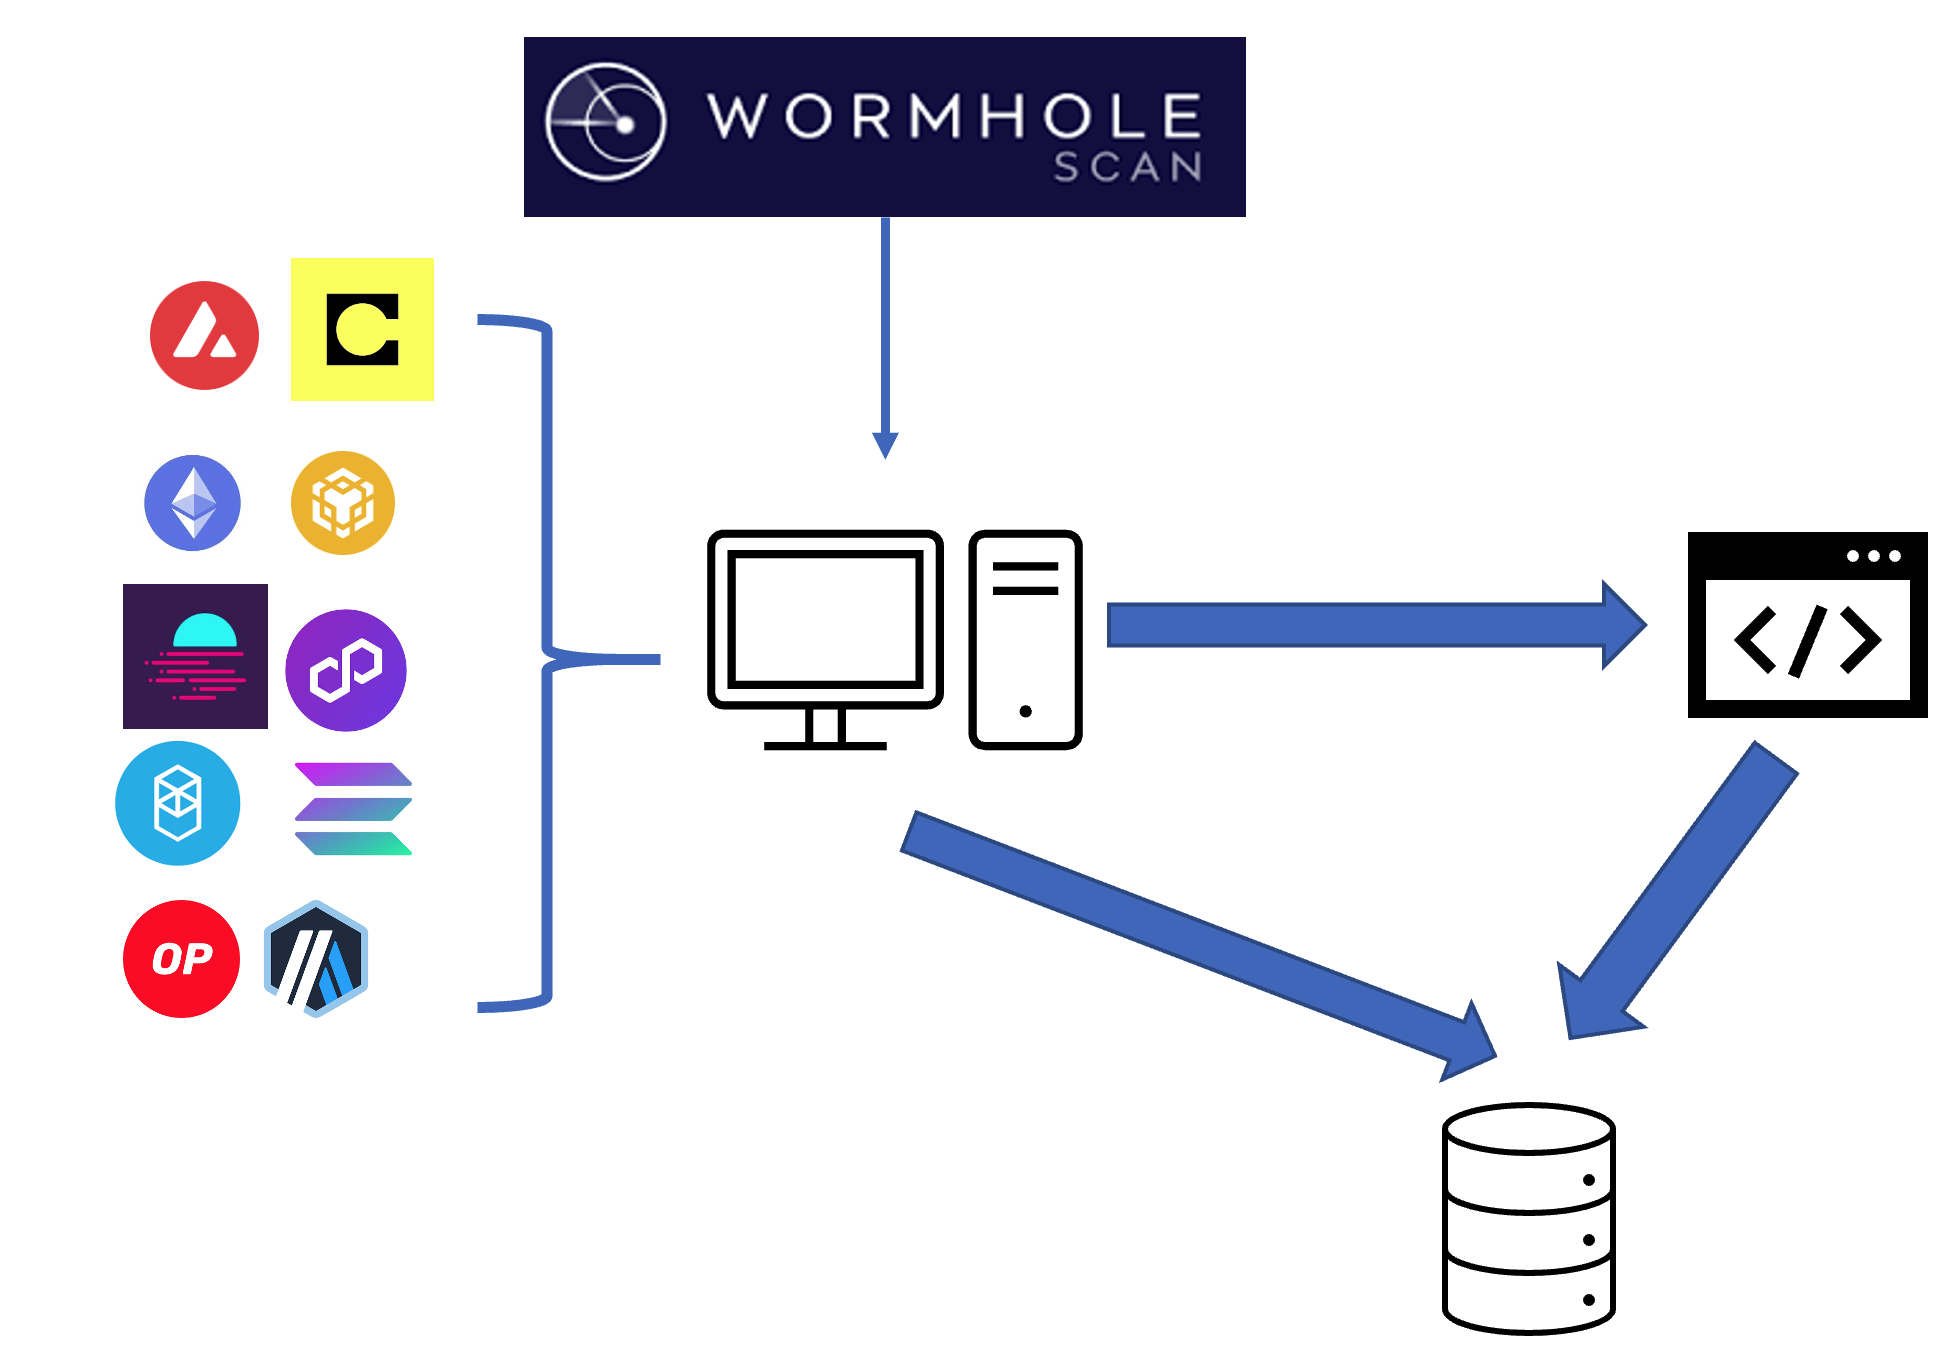
\includegraphics[width=\columnwidth]{fig/dbarch.pdf}
\caption{Live auditing system which consists of three components.}
\label{fig:live-audit-arch}
\end{figure}

%\subsection{Blockchain Monitor}
\textbf{Blockchain Monitor.}
%
The Blockchain Monitor obtains deposit and withdrawal transactions by
periodically retrieving the latest finalized blocks.  The Monitor
% primarily
uses the same commercial RPC services for collecting
Wormhole deposits and withdrawals as we used for the retrospective
analysis (Section~\ref{sec:retro-data}).\footnote{A fully operational
deployment would manage nodes participating in each of the blockchains
to obtain transactions in block data directly.}
%% However, this data
%% is not complete since a withdrawal transaction may reference a deposit
%% on a blockchain not supported by our system or pre-dates our data
%% collection (although infrequent, withdrawals do occur many months
%% after the deposit). To audit withdrawals like these, our system
%% retrieves their corresponding deposit transactions using Wormholescan, a
%% service maintained by Wormhole that indexes bridge
%% transactions. Wormholescan allows us to audit withdrawal transactions
%% whose corresponding deposits are not indexed by our system, improving
%% our audit coverage.\footnote{We note that Wormholescan occasionally
%% returns an error when queried for valid withdrawal transactions, as it
%% focuses on completeness on deposits since users need deposits
%% acknowledged to then trigger withdrawals. We have filed a bug report
%% with Wormhole.}
%% \deian{I would make clear if we actually need Wormholescan to be trustwhorthy or
%% not. I don't think we actually do (but later we bork) so worth clarifying (it
%% only really matters for availability). I would also prefix the Wormholescan
%% bit by saying the RC providers don't let you access ``very old'' events. And I
%% would end this discusison by saying that in practice you would run your own node
%% (which will let you query whatever you want however far back you want).}

% We also note that
The Monitor only retrieves finalized blocks since unfinalized blocks
may be reverted or reordered.  Since different blockchains have
different finality times, we use the timestamp of the latest finalized
block of Ethereum as the synchronization time since Ethereum has the
slowest finality time (around 12 minutes)~\cite{Finality:online}.
%% \footnote{Different systems may have thresholds for
%% finality, but usually wait for at least a few minutes.}
% We leave it to future work to explore how to synchronize to real time.
%% \elisa{It not super clear what the difference between the
%%   synchronization time (15 min) and the refresh time is. So with a
%%   sync time of 15, every time we audit, we are actually 15+10min
%%   behind?}
After retrieving the blocks, the Monitor extracts deposit and
withdrawal transactions for Wormhole and saves them to a local
database.

The polling interval is configurable and the Monitor polls chains
every 1 minute by default.  As a result, the live auditing system is
as recent as the polling interval combined with the finality time
--- a situation similar to bridges due to the polling nature of
distributed off-chain communication.
% We leave it to future work to optimize the delay further.

%% \alex{move wormholescan here.}

%% \geoff{this is the main effort because it needs to be extended for
%%   every chain that we want to audit?  this is where we should say that
%%   we monitor 11 chains (and name at least the popular ones), and
%%   something about why we don't monitor all chains supported by
%%   Wormhole (outside the scope of the approach (Bitcoin), not popular,
%%   etc., can point to previous discussion of which chains are out of
%%   scope.)}

% In addition, for withdraw transactions whose corresponding deposit transactions are on blockchains not supported by our system, we retrieve their corresponding deposit transactions using Wormholescan, a service that scans deposit and withdraw transactions for Wormhole. This setup allows us to audit any withdraw transaction whose corresponding deposit transaction is either on a supported blockchain or is indexed by Wormholescan. Overall, our system can currently audit over 99\% of the withdraw transactions on 11 blockchains, which collectively account for over 95\% of all withdrawal transactions on Wormhole. \alex{our undergrad is adding a blockchain called SUI, which will bump the number to 98\%. im not entire sure if this is necessary}

% The Blockchain Monitor component then extracts deposit and withdrawal transactions from the retrieved blocks. We use commercial RPC services to synchronize with the blockchains. Our system currently supports 11 blockchains, which together account for over 95\% of all withdrawal transactions on Wormhole. \alex{our undergrad is adding a blockchain called SUI, which will bump the number to 98\%. im not entire sure if this is necessary}
%One challenge here is that different blockchains have different finality times. Namely, if a block is not finalized, its transactions may be reverted or reordered. To address this, we always synchronize to the latest finalized block of Ethereum, which is the slowest to reach finality (around 15 minutes). We leave it to future work to explore how to synchronize all blockchains to real time. To bootstrap our database, we preload 2-week of transactions.


% The Blockchain Monitor component synchronizes all 11 blockchains up to a given time and extracts deposit and withdrawal transactions using commercial RPC services. One challenge here is that different blockchains have different finality times. Namely, if a transaction is not finalized, it may be reverted. To address this, we always synchronize to the latest finalized block of Ethereum, which is the slowest to reach finality (around 15 minutes). We leave it to future work to explore how to synchronize all blockchains to real time. To bootstrap our database, we preload 2-week of transactions.
% \alex{key challenge: sync to the same view}

%\subsection{Auditor}
\textbf{Auditor.}
%
For every new withdrawal transaction extracted by the Blockchain
Monitor, the Auditor attempts to find the corresponding deposit
transaction in its local database.  In most cases it will find the
deposit, but if it cannot find it (e.g., because the
withdrawal references a non-existent transaction), the Auditor sends
an email alert inviting manual inspection. If it finds a deposit, it
examines the deposit and withdrawal transactions, and sends an
alert if either the deposit has already been withdrawn (the new
withdrawal is double-spending) or the bridge transaction violates
the balance invariant.



% For every new withdraw transaction extracted by the Blockchain
% Monitor, the Auditor attempts to find the corresponding deposit
% transaction in its local database. If it cannot find the deposit, it

% The Auditor queries the local database to find the deposit transaction.
% In most cases it will find the deposit, but there are several reasons
% why a deposit transaction may not exist in the local database.  

% For
% example, the deposit transaction may pre-date our data collection
% (although infrequent, withdrawals do occur many months after the
% deposit), the deposit transaction may be on a blockchain that is not
% supported by our system, or the withdraw transaction may reference an
% invalid deposit transaction (e.g., Table~\ref{tab:xaction-hashes} in
% the appendix has examples of bridge transactions with invalid deposit
% references). 

%% \geoff{why not just use Wormholescan for everything, is there
%%   something we would miss, or is it a performance/cost optimization?}

%% Using Wormholescan expands our audit coverage to any withdraw
%% transaction whose corresponding deposit transaction is either in the
%% local stored by us locally or is indexed by Wormholescan.\footnote{}

%% Overall, our system can audit over 99\% of the withdraw transactions
%% on 11 blockchains, which collectively account for over 95\% of all
%% withdrawal transactions on Wormhole.

% There are several reasons why a deposit transaction may not exist in our local database. For example, it may be that the deposit transaction is too old and not stored in our database, or the deposit transaction may be on a blockchain that is not supported by our system.

%% For every withdraw transaction, if the deposit transaction is not
%% found, the Auditor component sends an email alert. If a deposit is
%% found, it then checks if the deposit has been withdrawn. If the
%% deposit has been withdrawn, it raises an alert. If the deposit has not
%% been withdrawn, it checks the invariant on the deposit and withdrawal
%% transactions. If the invariant is violated, the Auditor component
%% sends an alert.

% \alex{key challenge: missing data. and the fact that Wormhole has missing data}

%\subsection{Database}
\textbf{Database.}
%
The system uses a PostgreSQL database to store all information
regarding deposit and withdrawal transactions. This information
includes the transaction hash, the blockchain, the amount, and the
timestamp.  It also stores the auditing results, including whether the
deposit has been withdrawn and whether the invariant is
violated.
% \geoff{can be trimmed if we need space}


\subsection{Deployment}
%
We have deployed our live auditing system for the Wormhole bridge for a month.
%% in total starting on \geoff{date}.  \footnote{We report total days
%% because the system is on and off for data available issues and
%% bug-fixes.}
The system audits the deposit and withdrawal transactions between 10
blockchains, which collectively account for around 60\% of all
withdrawal transactions on Wormhole.  For the four weeks that our
system has been operational, it has audited over 60,000 transactions
in total (averaging more than 2,000 transactions per day). The system
currently refreshes every minute (configurable), and sends email
alerts if it observes a transaction violating the balance invariant or
another auditing property (e.g., the destination chain in the deposit
does not match the chain in the withdrawal).

In the time that our system has been operational, it has alerted on 22 transactions in six batches over four weeks. Upon manual inspection, we confirmed that all alerts were caused by previously unseen tokens (recall that in some cases we need to manually account for token-specific logic) or bugs in our code. Consistent with our retrospective analysis, the alert rate is very low at 0.03\% and raises fewer than one alert per day. This rate is on-par with other systems that have an alert budget (e.g., five alerts per day in the context of a lateral movement monitoring system~\cite{ho2021hopper}).
% In the time that we have had the system operational, it has alerted on
% multiple transactions that violated the invariant.  So far these
% transactions have proven to be errors in our implementation (e.g., failed to extract the correct amount) or the RPC services we used (e.g., not indexing a transaction).\alex{add numbers}\alex{add industry numbers}
% When manually inspecting the alerted transactions, we
% discovered that Wormholescan returned incorrect transaction data when
% compared with the transactions stored on-chain (prompting us to notify
% Wormholescan as mentioned above.)

In addition, while we have not observed any attacks during our
monitoring period, we simulated three attack scenarios to confirm that
the system alerts when expected.  These three transactions represent
three types of attacks: (1) a double-spend attack, (2) an
unbacked withdrawal attack, and (3) an attack where the deposit and
withdrawal amounts do not match. The system successfully alerted on
all three. % attacks.

% key: frequency are adjustable

%\section{Improved Architecture\\Incorporating into Bridges\\Protecting Bridges}
\section{Protecting Bridges}
\label{sec:active-protect}

Sections~\ref{sec:retro-results} and~\ref{sec:live-audit} showed how
applying the balance invariant can identify attacks retrospectively and
monitor ongoing transactions as an external third party without any
changes to existing bridge infrastructure.  However, the live
monitoring system only alerts on violations of the invariant and does
not prevent violating bridge transactions from being processed.

In this section, I describe an approach for extending an existing
bridge implementation to prevent malicious transactions from
executing.  Our goal is to present a proof-of-concept implementation
to demonstrate the feasibility of applying the balance invariant in the
workflow of bridge transactions as an active defense against malicious
transactions.  I acknowledge that several practical issues remain
for a complete operational system, presenting an opportunity for
interesting future work.

%% explore the question of whether it is possible to implement a
%% mechanism that stops malicious transactions from execution with
%% minimal code changes.

% how hard it would be to modify the Wormhole bridge to prevent transactions that violate the invariant from being processed. I propose an improved architecture that treats the bridge relaying infrastructure as a black box and can effective stop any malicious transactions that break the invariant and caused by code bugs.

% Below, I start by answering the question of where to introduce the mechanism. Then, using Wormhole as an example, I show how I can modify the bridge to prevent malicious transactions from being processed with fewer than 30 lines of code changes. Finally, I evaluate the security and performance of the improved architecture.

I start by proposing a new model for the workflow of bridge
transactions.  Then, using Wormhole as an example, I show how to
modify an existing bridge implementation to prevent malicious transactions from
being processed with fewer than 30 lines of code changes.  Finally, I
evaluate the correctness and overhead of this initial implementation.

\subsection{The Announce-then-Execute Model}

To guide the design of a new model, I first highlight where the
attack surfaces exist. As shown in Figure~\ref{fig:cross-chain}, a
vulnerability can exist in as early as the second step (verify lock
amount) to as late as the next-to-last step (verify relayed
transaction). Thus, a natural place to introduce a protection
mechanism is just before the final step, which executes the relayed
transaction.

Using this insight I propose an announce-then-execute model.
Figure~\ref{fig:improved-arch} depicts the entities and steps involved
in the new model, focusing on the destination chain (replacing the
right-most box of Figure~\ref{fig:cross-chain}).  The new model
employs two steps to process a withdrawal transaction: (1) verify and
announce the withdrawal transaction on the destination blockchain (steps
8 and 9) and (2) execute the withdrawal transaction (steps 11 and
12). Of particular note, this new model introduces an additional
entity, the \emph{Approver}, which is responsible for approving the
relayed transaction before it is executed.  The Approver can be a bridge
operator, a trusted or trustless third-party (e.g., Bascule~\cite{bascule},
inspired by our work, uses trusted execution environments instead of consensus to ensure the safety of the approver), or a set of
third-parties (e.g., using
multisig for decentralized control). It is responsible for
verifying that the announced withdrawal transaction satisfies the
invariant by validating the same conditions as the Auditor in the live
monitoring system (Section~\ref{sec:live-audit}).  If the relayed
transaction violates the invariant, the Approver can reject the
transaction to prevent it from being executed.

% In addition, I observe that many bridges (e.g., Wormhole) couple the last two steps tightly --- the verification and execution of the relayed transaction are done in the same function call. While being gas efficient, this implementation has a critical drawback. Namely, if the verification function has a bug, it would be impossible to stop the malicious transaction from being executed.

% This means that the verification of a relayed transaction is done at the same time as the execution of the relayed transaction. 

\begin{figure}[t]
\centering
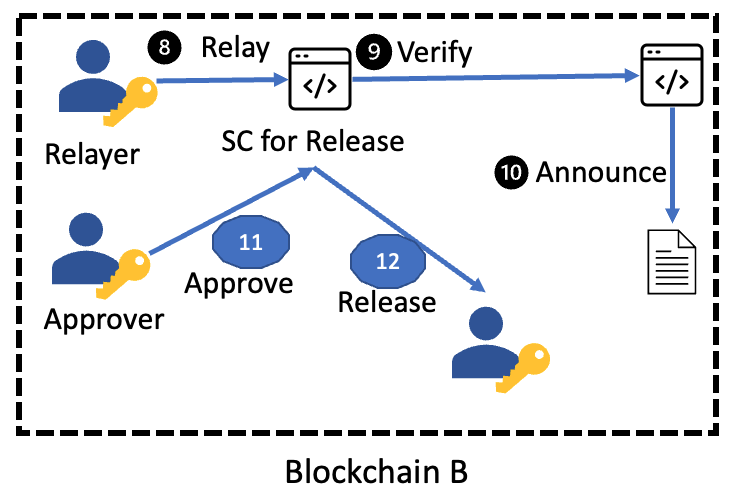
\includegraphics[width=0.9\columnwidth]{fig/improved.pdf}
\caption[Announce-then-Execute Model for Bridges]{Announce-then-execute model for bridges. The approver verifies the relayed transaction before its execution. The approver can be implemented differently (e.g., a set of third-parties), depending on the desired security properties.}
\label{fig:improved-arch}
% \vspace{-0.1in}
\end{figure}


\subsection{Threat Model, Assumptions, and Trade-offs}
I assume that the approver is able to independently verify the relayed transaction and the correct amount of tokens to be transferred. Under this assumption, the announce-then-execute model prevents any implementation bug in any existing bridge components, from step 2 (e.g., the bridge fails to compute the correct deposit amount) to step 8 (e.g., the bridge fails to verify the signature of a relayed transaction). Further, if the 
approver uses secure hardware (namely, HSMs) or a decentralized third-parties
(e.g., with multisig), the model can provide additional protection against
insider threats and key theft (e.g., up to the multisig threshold). Of course,
if the bridge is the only approver, the model does not provide any additional
protection against such insider threats or key theft attacks.


The announce-then-execute model has a few advantages. First, it
explicitly separates the verification and execution of the relayed
transaction, thereby providing an opportunity to reject transactions
that violate the balance invariant.  In comparison, many bridges (e.g.,
Wormhole) couple the last two steps tightly --- the same function call
performs both the verification and execution of the relayed
transaction.  As a result, if the verification step has a bug, it is
not possible to stop violating transactions from being
executed.

Second, the announce-then-execute model allows any external
party, that has visibility into both blockchains, to determine if the
relayed transaction violates the invariant. A long-standing challenge
with bridges is the oracle problem: the destination blockchain does
not have visibility into the source blockchain. The
announce-then-execute model side-steps the oracle problem by allowing
an external party to verify the relayed transaction before it is
executed. This external party can be the bridge operator or a group of third-parties.
Moreover, the announce-then-execute model is compatible with
existing bridges, as it only requires modification to the last step
and treats the relaying infrastructure as well as the verification
code as a black box. In fact, Wormhole's implementation on Solana already separates the process of verifying and executing the relayed transaction, making it even easier to adopt the announce-then-execute model. Had they implemented the announce-then-execute model, the Wormhole bridge would have been able to prevent the \$360M attack on the Solana network~\cite{wormholeattack}.

Lastly, the announce-then-execute model does not
introduce any new attack surfaces --- even if the approver naively
approves all transactions, an attacker still has to exploit other
vulnerabilities in the bridge to profit.

\subsection{Implementation}

%% I took open-sourced Wormhole code written in solidity and modified it to implement the announce-then-execute mechanism.
%% Wormhole's current withdraw function performs two tasks:
%% it verifies the signatures that authorize the withdraw transaction and then executes the withdraw transaction. I split the withdraw function into two separate functions: \texttt{announceWithdraw} and \texttt{approveWithdraw}. The \texttt{announceWithdraw} function handles signature verification and announces the withdraw transaction on the destination blockchain, while the \texttt{approveWithdraw} function executes the withdraw transaction. This modification required fewer than 30 lines of code changes.

Continuing our focus on Wormhole from Section~\ref{sec:live-audit}, I
modified one of Wormhole's open-source contracts to implement the
announce-then-execute model.  Wormhole's current withdrawal function
performs two tasks: it verifies the signatures that authorize the
withdrawal transaction, and then executes it. I
split the withdrawal function into two separate functions:
\texttt{announceWithdraw} and \texttt{approveWithdraw}. The
\texttt{announceWithdraw} function handles signature verification and
announces the withdrawal transaction,
while the \texttt{approveWithdraw} function executes the withdrawal
transaction. This modification required fewer than 30 lines of code
changes.

For simplicity, I opted for a single approver with one key in our implementation. However, our implementation can be easily extended (e.g., to use multisig). In addition, while our implementation has not been adopted by the Wormhole team (as I are a research group not affiliated with Wormhole), our solution has inspired other industry projects to adopt a similar approach~\cite{bascule}.

\subsection{Evaluation}

As a final step I performed a high-level evaluation of the
correctness and overhead (in terms of gas usage) of the
announce-then-execute implementation.  I deployed our bridge
implementation on the Binance and Fantom testnets due to the
availability of free faucets for acquiring testnet tokens for them.
I then executed a series of benign and malicious transactions using
Binance as the source chain and Fantom as the destination chain.

% , and tracked their gas usage during execution.

%% (would be fine if this were a long eval, but since it's so short it's
%% not really needed)
%%
%% I demonstrate that the improved architecture
%% can effectively stop all three malicious transactions while allowing
%% benign transactions to proceed. I also show that the overhead of the
%% improved architecture incurs only a moderate overhead of 50\% more gas
%% usage without any optimization.

\textbf{Correctness.}  For evaluating correctness I disabled the
security checks in the original implementation (e.g., signature
verification) to allow malicious transactions to flow through the
contract implementation (e.g., simulating key compromise).  I then
executed 100 pairs of deposit and withdrawal transactions to validate
that the implementation correctly identifies and protects itself
against malicious transactions that violate the balance invariant.

All but three of the 100 paired transactions were benign, and used
randomly generated values as transaction inputs.
%
The remaining three paired transactions were malicious and were
randomly placed in the transaction sequence.  The malicious
transactions represented the three kinds of bugs underlying the
large attacks in Section~\ref{sec:retro-results}: (1) a bug that
allows a user to withdraw more tokens than they deposited, (2) a bug
that allows a user to withdraw tokens without depositing any
(simulating key compromise), and (3) a bug that allows a user to
withdraw twice from the same deposit (double spending).

The bridge implementation correctly executed the benign transactions
to completion and rejected the three malicious transactions.  The
results are the same independent of where the malicious transactions
randomly appear in the sequence.

\textbf{Overhead.}  The additional steps add overhead to implementing
bridges.  For this experiment, I measured the gas usage for executing
Wormhole's original implementation (with its security checks) and the
gas usage of the announce-then-execute implementation (also with the
original security checks plus our added code).  On average, our
proof-of-concept implementation consumed 110\thou more gas than the
original implementation (370\thou vs.\ 260\thou gas) when
executing the benign transactions, which translates to a
roughly \$1 increase for a typical withdrawal on Ethereum.
% a 50\% increase in gas usage.

I note that our implementation is not optimized for gas usage, and
these results indicate that an
% real
operational deployment
% of the announce-then-execute model
will likely want to reduce the gas overhead of
the additional work (e.g., narrowing to transactions above a threshold
amount of funds).  As discussed further in Section~\ref{sec:discuss},
such optimizations and other practical issues of a real deployment are
interesting future work.


\section{Related Work}
% * Bridge specific\\
% * Cross-Chain Security\\
% * Transaction-based Analysis\\
% * Industry Efforts\\

%% Start with the most relevant ones, and other ones can be added later

% \alex{this needs to be written.}
% Focus: Transaction-based Analysis
Blockchains are, by their nature, public and thus support direct
empirical analysis of past transactions.  This property has engendered a rich
literature quantifying and characterizing a range of quasi-adversarial
activities on \emph{individual} blockchains including
arbitrage~\cite{mclaughlin2023large, qin2022quantifying}, sandwich
attacks~\cite{qin2022quantifying, zhou2021high},
frontrunning~\cite{daian2020flash}, transaction
replays~\cite{qin2022quantifying}, and a range of smart contract
vulnerabilities and attacks~\cite{perez2021smart,grossman2017online,
  rodler2018sereum, zhang2020txspector, wu2021defiranger,
  ferreira2021eye}.  While our work focuses on the cross-chain
context, a number of the vulnerability classes
identified in such work are directly implicated in the attacks I analyze.%\alex{additional related work}

%and counter-attacks~\cite{zhang2023your}. Unlike this line of work, I employ a% similar method but focus exclusive on cross-chain bridges.


% Another domain of research explorer the possibility of monitoring blockchains live. probably not necessary

% Another domain of research studies cross-chain bridges, but not the security aspect. 

In the cross-chain context, there are several different streams of
related work.  First are the efforts to improve the security and
performance of cross-chain bridge designs --- particularly in managing
cross-chain consensus concerning state changes --- using
zero-knowledge~\cite{xie2022zkbridge} or committees of
validators\cite{lan2021horizon,li2022polybridge}.
Some many-chain blockchain ecosystems (e.g., Avalanche) are extending
their chains with built-in bridges (across different chains). I consider our
work orthogonal to these efforts as I focus on unbalanced bridge transactions, independent of the particular
security violation that allowed such an outcome to take place.
Indeed, some of the compromised bridges did use sets of validators.

Another line of work has reviewed real-world attacks on
cross chain
bridges\cite{lee2023sok,zhang2023sok,notland2024sok,zhao2023comprehensive}
--- ranging from just a few such events to an analysis of over 30
attacks.  Our work has directly benefited from the insight and
documentation these authors provide, but our respective focus is
distinct.  While these efforts have concentrated on identifying
the vulnerabilities and mechanisms of attack, our work is
agnostic to these details and focuses on the financial
side-effects those actions.

Yet a third research direction seeks to automatically discover new
vulnerabilities in cross-chain bridges.  Some examples of this work
use machine learning such as ChainSniper~\cite{tran2024chainsniper},
which trains models to identify vulnerable smart contracts, and Lin et
al.~\cite{lin2024detecting}, who train models to detect fake deposit
events.  Other examples use static analysis such as
XGuard~\cite{wang2024xguard}, which statically analyzes bridge
contracts for inconsistent behaviors, and
SmartAxe~\cite{liao2024smartaxe}, which analyzes the control-flow
graph of smart contracts and identifies access control and semantic
vulnerabilities.

The papers philosophically closest to ours are those that consider the
security properties of cross-chain bridges at a higher-level of
abstraction.  For example, Belichior et
al.~\cite{belchior2023hephaestus} build and evaluate a synthetic
bridge designed to allow high-level monitoring of bridge behavior --- including variations in financial state.  In
a more empirical context, Huang et al.~\cite{huang2024seamlessly}
characterize the transactions of the Stargate bridge, and highlight
the correlation between large or unusual trades and individual attacks.  Finally, perhaps the closest work to our own is Zhang et
al.'s XScope~\cite{zhang2022xscope} which models real-world bridge bugs using a set of
pre-defined rules and applies these empirically to identify several attacks retrospectively. Like our work, they focused on invariant patterns rather than the low-level details of
smart contract bugs. 
%
That said, the rules considered by XScope are still considerably lower-level and more granular than our balance invariant as they are seeking to identify the cause of the detected attacks that have taken place.
% \footnote{There are still many benefits to this approach.  For example, they are able to identify transactions that are out-of-scope for our approach. Notably, they identified
% four deposit transactions that were previously unreported. These four deposit transactions did not have corresponding withdrawal transactions and therefore considered out-of-scope.}  
While the two efforts are complementary, I believe
our work is simpler to understand and implement, more clearly robust
(we have tested against a far wider range of bridges and blockchains),
and, as a result, is likely more attractive for inline deployment.


% The rules considered by XScope are considerably lower-level and more granular than our balance invariant as they are seeking to identify the cause of the detected attacks that have taken place but, like us, they are
% more focused on invariant patterns than the low-level details of
% % smart contract bugs.  While two efforts are complementary, I believe
% our work is simpler to understand and implement, more clearly robust
% (we have tested against a far wider range of bridges and blockchains)
% And, as a result, is likely more attractive for inline deployment.




 % Another thread of research has focused on statically analyzing the smart contracts of cross-chain bridges. This includes . % Both papers rely exclusively on static techniques and do not consider any actual transactions. 

Finally, a range of blockchain companies advertise tools that actively
monitor cross-chain bridge transactions for anomalies.  These include
Hexagate~\cite{Hexagate75:online}, Hypernative~\cite{Hypernative:online}, PeckShield~\cite{PeckShie48:online}, Slowmist~\cite{SlowMist92:online}, Certik~\cite{CertiKWh86:online} and ChainAegis~\cite{ChainAeg18:online} (among
others), all of which claim various levels of automated alerting for
suspicious transactions.  However, without clear information on how
these systems operate, or empirical results on their efficacy, it is hard to relate our work to those tools beyond our shared goals.

%Beyond various academic efforts, industry has also developed web3 tools that actively monitor ongoing transactions on cross-chain bridges. An example is Hypernative, which provides real-time monitoring and protection for bridges.\alex{mostly for deian} Without any public information on how Hypernative works, it is unclear how it compares to our work. Other platforms, such as PeckShield, SlowMist, CertiK and ChainAegis, have offered generic alerts for suspicious transactions. Given the volume of alerts generated, it is unclear how many of them are false positives.

% Other cross chain solutions. Also, limitations 

% This include hypernative, which monitors transactions on Ethereum and Binance Smart Chain, and Chainalysis, which provides a wide range of tools for monitoring transactions on various blockchains.


% Huang et al. analyzed the transactions of Stargate, but did not examine the security aspect of these transactions.

% and XScope, which models pre-defined bugs. Both papers rely exclusively on static analysis and do not consider the actual transactions. Huang et al. analyzed the transactions of Stargate, but did not examine the security aspect of these transactions.
% Other papers have tried to statically analyze cross-chain bridges. This includes XGuard, which statically analyzes bridge contracts and identifies inconsistency behaviors, SmartAxe, which identifies access control vulnerabilities and semantic inconsistency. Both papers rely exclusively on static analysis and do not consider the actual transactions. 
% XScope, which models a pre-defined bugs, is the most closest to us in that it also involves examining real-world transactions. Another line of work uses machine learning to detect vulnerabilities, such as ChainSniper and Lin et al.
% Huang et al. analyzed the transaction of stargate, but does not examine the security aspect of these transactions.

% Of particular note, the first two papers do not investigate any transactions, while the last one analyzed two million transactions on Ethereum. These papers can effectively find previously 

% The stream of research most relevant to our work focuses on the security of cross-chain bridges. Concretely, Lee et al., Zhang et al., Notland et at., and Zhao et al., have all systematically analyzed real-world attacks against cross-chain bridges. 
% While the number of examples and bridges studied varies (from a few to over 30), they all take the perspective of \textit{individual vulnerabilities}. Our work builds on top of this line of research by providing a simple variant that captures a large portion of these vulnerabilities.
 
% , on the other hand, unifies a large portion (but not all) these vulnerabilities into a single invariant that captures the security of cross-chain bridges.

% including understanding various phenomenons, detecting attacks, and validating academic tools. As an example, Daian et al.~\cite{} quantified the prevalence of front-running attacks on Ethereum by studying transactions of a selected set of exchanges.


% transactions to quantify the prevalence of  on Ethereum. Similarly, Tran et al.~\cite{} used transactions to understand the behavior of smart contracts.

% A rich literature has utilized Ethereum transactions for a variety of tasks, including understanding the runtime behavior of smart contracts, vulnerability detection, and validation of academic research.

% tapped into the rich resource of Ethereum transactions for understanding the runtime behavior of smart contracts, vulnerability detection, and validation of academic research.

% Transactions provide a rich source of information 
% for understanding the runtime behavior of smart contracts, vulnerability detection, and validation of academic research. Unsurprisingly, a rich literature has tapped into this resource.

% . Tools that detect specific vulnerabilities.
% ECFChecker~\cite{grossman2017online} is one of the first tool that analyzes Ethereum transactions and determines if an execution is Effectively Callback Free. Sereum~\cite{Sereum} detect re-entrancy attacks. TxSpector~\cite{TxSpector} detect user-supplied rules. Others have used it for price manipulation~\cite{DEFIRANGER} and exploitation~\cite{Smart Contract Vulnerabilities}

% security of cross-chain bridges. In this section, I review related work on cross-chain bridges, cross-chain security, transaction-based analysis, and industry efforts.


\section{Ethics}
\label{sec:ethics}

We believe our work, which deals with public data, no identified
individuals and a simple means for identifying attacks on crypto token
transfer bridges (and potentially preventing such attacks in the
future), has very low ethical risk and significant upside. Moreover, I have attempted to disclose significant suspicious bridge
transactions to appropriate bridge operators (yet with limited
success as most of the bridges have ceased operations). Lastly, I will make our code and data available upon publication.
% 
% We strictly use public data and to
% the extent that I identify outcomes (e.g., attacks) they are at the
% granularity of bridges and blockchains, not individuals.

% As well,


% Considering the Menlo report principle of ``Respect for Persons'', we
% are not dealing with, nor do I attempt to analyze, data at the
% granularity of individual persons.  We strictly use public data and to
% the extent that I identify outcomes (e.g., attacks) they are at the
% granularity of bridges and blockchains, not individuals.  Similarly,
% with respect to the principle of ``Justice'', I have no reason to
% believe that our analysis discriminates at the level of persons or
% distinct groups of persons --- all users of bridges should benefit
% equally (excepting criminals).  On the topic of ``Respect for Law and
% Public Interest'', I are engaging with existing public data, I have
% documented our methods clearly and I are careful to limit our factual
% statements to those for which I have evidence.  As well, I have made
% a point to disclose significant suspicious bridge transactions to appropriate
% bridge operators.


% We believe our work, which deals with public data, no identified
% individuals and a simple means for identifying attacks on crypto token
% transfer bridges (and potentially preventing such attacks in the
% future), has very low ethical risk and significant upside.  However,
% in the interest of due diligence, I provide a more thorough
% justification of this position following the Menlo Report principles
% as indicated by the USENIX Security call.

% Considering the Menlo report principle of ``Respect for Persons'', we
% are not dealing with, nor do I attempt to analyze, data at the
% granularity of individual persons.  We strictly use public data and to
% the extent that I identify outcomes (e.g., attacks) they are at the
% granularity of bridges and blockchains, not individuals.  Similarly,
% with respect to the principle of ``Justice'', I have no reason to
% believe that our analysis discriminates at the level of persons or
% distinct groups of persons --- all users of bridges should benefit
% equally (excepting criminals).  On the topic of ``Respect for Law and
% Public Interest'', I are engaging with existing public data, I have
% documented our methods clearly and I are careful to limit our factual
% statements to those for which I have evidence.  As well, I have made
% a point to disclose significant suspicious bridge transactions to appropriate
% bridge operators.

% Finally, on the topic of ``Beneficence'', we
% identify the three sets of stakeholders in our work.  These include
% the past and (potential) future victims whose investments, both direct
% and indirect, via token transfer bridges have been undermined by
% large-scale thefts from these services.  In addition, other
% stakeholders include bridge operators and, finally, the criminal actors who
% derive income from vulnerabilities in bridges.  We argue that our
% retrospective analysis creates no direct new harm for any parties ---
% these attacks have already happened.  For bridge operators, our
% analysis may create some potential liability in supporting a civil
% claim of poor stewardship, but at the same time our documentation of
% the widespread nature of this problem provides a ``common practice''
% defense.  Some of the unilateral transfers I have documented, if they
% were illegitimate (which I do not know), could also create liability
% for bridge operators, but I believe this potential harm is balanced
% against the interest of investors in transparency and fairness in
% operating financial services.  Finally, for our proposed real-time
% analysis approaches, if these were adopted by bridge operators, it
% could foreclose a broad range of attacks.  We admit that this outcome
% could harm our criminal stakeholders as it might deny them of an
% important income stream.  Knock on effects could include a reduction
% in revenues for online crypto money laundering services and Lamborghini
% dealerships, but I believe this is well-justified by the concordant
% reduction in victimization.



\section{Discussion and Future Work}
% Things I'd like to mention:   
    % Challenges in identifying the amount
    % Benefits of the new architecture

\label{sec:discuss}
% \alex{add more sections. e.g., add-on}
Our work is a ``first cut'' at identifying, validating and implementing a
generic mode of theft protection into cross-chain transactions. We show that a
simple balance invariant is sufficient to detect and prevent most bridge
attacks. Our effort also highlights the need for better auditability and
auditing in the bridge ecosystem, and for new bridge designs.  Indeed, deploying a cross-chain token bridge with an in-line balance invariant
monitor is an open challenge.

As mentioned in Section~\ref{sec:background}, in this chapter I focus on
cross-chain token bridges and thus our approach does not directly apply to
bridges that have built-in exchanges and swaps.  Still, similar
invariant-checking techniques likely extend to such \emph{cross-chain exchanges}
and similar protocols (e.g., Automated Market Makers which trade between a
range of cryptocurrencies in decentralized exchanges). Such extensions will
require incorporating contemporaneous price oracle data
into our framework
and addition reasoning.
% We leave this to future work.

The larger opportunities opened up by this work are
more architectural.  Today, when a crypto platform declares that their
system has been audited, they typically are referring to a third-party
that inspects their smart contracts for common logic errors or
deficiencies in their process.  Any validation of overall financial
safety is inherently entwined with the totality of the implementation.
However, such code-oriented audits are inherently challenging and
ill-suited for overarching questions of financial risk.  They must
evaluate all contracts and bridge code that directly or indirectly
have access to keys controlling assets and then must ensure that no
combination of inputs or invocations might lead to a loss (itself an
outcome that is rarely well defined \emph{a priori}).  Unsurprisingly,
multiple bridges in our study had been previously audited by third
parties before their attacks.

Our work suggests that by separating overall financial safety
invariants from the intricate details of every given contract or
trade, I can dramatically simplify the defender's job and their
ability to reason about risk.  Similar to so-called ``circuit
breakers'' implemented in traditional securities exchanges, or the
atomic repayment guarantees embedded in single-blockchain ``flash
loan'' services, the ability to script overarching financial
constraints independent of transaction details can be extremely
powerful.  For example, one might extend this work beyond a simple
cross-chain balance invariant to enforce limits on liquidity losses or
to place limits on collateralization risk for tokens backed by
stablecoins.  We hypothesize that by centralizing the specification and
enforcement of \emph{overall} financial constraints in one place, they
will be far easier to audit and reason about.


Chapter~\ref{chap:bridge}, in part, has been submitted for publication of the material as it may appear in Proceedings of the Network and Distributed System Security Symposium 2026. Enze Liu, Elisa Luo, Jian Chen Yan, Katherine Izhikevich, Stewart Grant, Deian Stefan, Geoffrey M. Voelker, and Stefan Savage. The dissertation author was the primary investigator and author of this paper.
% \alex{
% * Bridge support for auditing. 
% * From a design perspective
%     * Whats emitted
%     * Easy indexing?
%     * From a transaparency perspective
%        * What addresses
% * Talk about arichtectural designs and tradeoffs
% * Scenarios in the broader context of bridges (like swap)
% }

% \section{Conclusion}
% In summary, I have empirically shown, by analyzing 20 million
% transactions over 11 bridges and 21 blockchains, that a simple balance
% invariant---checking that value is conserved cross-chain in a bridge
% transaction---is sufficient to identify every such attack I have
% encountered.  Moreover, almost every violation of the balance
% corresponds to a bridge transaction that deserves further manual
% scrutiny (i.e., the ``false positive'' overhead is extremely minimal).
% We show, via proof-of-concept implementations that detection based on
% this principal is cheap to implement and can be performed in
% real-time, either in parallel for the purpose of alerting, or in-line
% to prevent violating transactions from being completed---an approached
% that would have likely foreclosed the \$US2.6B+ in claimed losses from
% prior attacks.  Finally, I argue that accounting-orientated defenses such as ours may be a powerful tool for managing risk in a range of decentralized finance contexts.

% Bridge support for auditing. 
    % From a design perspective
        % Whats emitted
        % Easy indexing?
    % From a transaparency perspective
        % What addresses
    
    % Talk about arichtectural designs and tradeoffs

% Apply scenarios in the broader context of bridges (like swap)


%* no single place with all the bridge contracts (undocumented contract addresse%s)\\
%* relying on external states / third-party api\\
%* internal transaction\\
%* rpc services (internal service, availability, weird corner cases such as arbi%trum)\\
%* talk about the benefits of new architecture (e.g., clear announce as well as %support revert and support advanced debugging / simulation)\\
%* Logs are truncated too for solana (fix 2023) \\
%* Learning based approach for bridge/token behavior?\\
%\subsection{Limitations}
%* We only consider designated withdraw functions. If you withdraw tokens by directly calling Transfer, I cannot detect it. Similarly, if you repurpose other functions (e.g., deposit) for withdrawal, I cannot detect it.\\
%* We only prevent bridge from losing money. Future work can consider adopting the user-centric perspective and model the end-to-end flow by taking into consideration bridge- and token-specific logics.
%* Other attack vectors exist.\\
%\subsection{Counter Measures}





% For example, I only consider designated withdraw functions. If you withdraw tokens by directly calling Transfer, I cannot detect it. Similarly, if you repurpose other functions (e.g., deposit) for withdrawal, I cannot detect it.  We also only prevent the bridge from losing money. Future work can consider adopting the user-centric perspective and model the end-to-end flow by taking into consideration bridge- and token-specific logics.  Finally, other attack vectors exist that are not captured by our approach.  For example, a bridge could be used to launder money by transferring tokens back and forth between two accounts.  While our approach would detect the loss of funds, it would not detect the money laundering.  However, I believe that our approach is a valuable first step in protecting bridges from theft and that it can be extended to address these and other vulnerabilities in the future.
% We only consider designated withdraw functions. If you withdraw tokens by directly calling Transfer, I cannot detect it. Similarly, if you repurpose other functions (e.g., deposit) for withdrawal, I cannot detect it.\\
%* We only prevent bridge from losing money. Future work can consider adopting the user-centric perspective and model the end-to-end flow by taking into consideration bridge- and token-specific logics.
%* Other attack vectors exist.\\



\chapter{Conclusion}

This dissertation explores the problems and solutions for sharing disaggregated memory. The high
access latency and extreme cost of contention in far-memory over RDMA cause many data structures,
which would otherwise be efficient, to experience performance collapse. Stale caches cause
opportunistic data structures to fail under contention, and pointer-based data structures incur
additional round trips when far-memory pointers need to be resolved. Using existing techniques,
applications can be made to work, but they simply have to incur the penalties of sharing when under
contention.

\begin{center}
\textit{Data structures can be optimized for disaggregated memory by leveraging network programmability} \\
\end{center}


In this chapter we begin by summarizing the contributions of this dissertation and their
relationship to our thesis claim, and we conclude with a discussion of this works limitations paired
with future work directions in this area of research.

\section{Contributions}

In this dissertation, we have contributed to the state of the art in disaggregated memory systems by:

\begin{itemize}
    \item Demonstrating the significant performance gains achievable by using a programmable switch to cache the contended state of a data structure and resolve the conflicts in the network.
    \item Showing that a programmable switch can reduce the instruction-level bottlenecks of RDMA atomic operations.
    \item Demonstrating that through locality optimizations locks can be fit into a small amount of NIC memory.
    \item Showing that RDMA-verbs are well suited for locality optimized data structures.
\end{itemize}

We believe that these contributions are significant stepping stones towards the design of future
efficient disaggregated systems. In the case of {\sword}, which demonstrated acceleration on
list appends, it could be adapted to other data structures with similar properties, for example,
log-structured systems. We believe that the insight behind RCuckoo's locality-based optimizations is
general and that many data structures could benefit from localizing their data in a similar fashion.

\section{Future Work}


Each of the works presented in this dissertation is a step towards more efficient disaggregated
systems. In this section, we speculate on future directions for this area of research based on the
limitations of the work presented here.

The future for disaggregated systems is bright. This work has demonstrated that shared remote memory
can be made efficient with programmable networking hardware and that, through careful design, data
structures can be adapted to disaggregated memory. Hopefully, future work will build on these
techniques and enable a shift towards mainstream disaggregated computing.




\appendix
% \Blinddocument
\bibliographystyle{plain} % Or whatever style you want like plainnat

\bibliography{thesis}

% Stuff at the end of the dissertation goes in the back matter
\backmatter

\end{document}
